%%%%%%%%%%%%%%%%%%%%%%%%%%%%%%%%%%%%%%%%%%%%%%%%%%%%%%%%%%%%%%%
%% OXFORD THESIS TEMPLATE

% Originally by Keith A. Gillow (gillow@maths.ox.ac.uk), 1997
% Modified by Sam Evans (sam@samuelevansresearch.org), 2007
% Modified by John McManigle (john@oxfordechoes.com), 2015
% Modified by Maud Gautier (https://github.com/MaudGautier), 2019
% Modified by Thibault Latrille (https://github.com/ThibaultLatrille), 2020
%
% This version Copyright (c) 2020 Thibault Latrille
%
% Broad permissions are granted to use, modify, and distribute this software
% as specified in the MIT License included in this distribution's LICENSE file.

%%%%% CHOOSE PAGE LAYOUT
%\documentclass[a4paper,openright,twoside]{thesis}
\documentclass[a4paper,oneside,nobind]{thesis}

\definecolor{Nonpolar}{HTML}{fef1d2}
\definecolor{Polar}{HTML}{a9fdd8}
\definecolor{Basic}{HTML}{d7f8ff}
\definecolor{Acidic}{HTML}{feceea}
\definecolor{Stop}{HTML}{D0D0D0}


\definecolor{RED}{HTML}{EB6231}
\definecolor{YELLOW}{HTML}{E29D26}
\definecolor{BLUE}{HTML}{5D80B4}
\definecolor{LIGHTGREEN}{HTML}{6ABD9B}
\definecolor{GREEN}{HTML}{8FB03E}
\definecolor{PURPLE}{HTML}{BE1E2D}
\definecolor{BROWN}{HTML}{A97C50}
\definecolor{PINK}{HTML}{DA1C5C}

\newcommand{\der}{\mathrm{d}}
\newcommand{\e}{\mathrm{e}}
\newcommand{\dnds}{dNdS}
\newcommand{\indice}{l}
\newcommand{\indiceexp}{^{(\indice)}}
% Time, effective population size and mutation rate.
\newcommand{\Ne}{N}
% \acrshort{DNA}
\newcommand{\SetNuc}{\Omega_{\mathrm{N}}}
\newcommand{\SetWeak}{\Omega_{\mathrm{W}}}
\newcommand{\SetStrong}{\Omega_{\mathrm{S}}}
\newcommand{\mutmatrix}{R}
\newcommand{\Mutmatrix}{\bm{\mutmatrix}_{4\times4}}
\newcommand{\exchan}{\rho}
\newcommand{\Exchan}{\bm{\exchan}_{6\times1}}
\newcommand{\mutequi}{\sigma}
\newcommand{\Mutequi}{\bm{\mutequi}_{4\times1}}
% Codons
\newcommand{\SetCodon}{\Omega_{\mathrm{C}}}
\newcommand{\ci}{{i}}
\newcommand{\cj}{{j}}
\newcommand{\itoj}{\ci, \cj}
\newcommand{\nucitoj}{\mathcal{M}(\itoj)}
\newcommand{\submatrix}{Q}
\newcommand{\Submatrix}{\bm{\submatrix}_{61\times61}}
\newcommand{\subequi}{\pi}
\newcommand{\Subequi}{\bm{\subequi}_{61\times1}}
\newcommand{\probmatrix}{P}
\newcommand{\Probmatrix}{\bm{\probmatrix}_{61\times61}}
% Amino-acids
\newcommand{\SetAa}{\Omega_{\mathrm{A}}}
\newcommand{\Neighbor}{\mathcal{V}}
\newcommand{\NonSyn}{\mathcal{N}}
\newcommand{\Syn}{\mathcal{S}}
\newcommand{\Nx}{\Neighbor_x}
\newcommand{\NxAB}{\Neighbor_x^{\mathrm{A} \rightarrow \mathrm{B}}}
\newcommand{\NyBA}{\Neighbor_x^{\mathrm{B} \rightarrow \mathrm{A}}}
\newcommand{\NxWS}{\Neighbor_x^{\mathrm{W} \rightarrow \mathrm{S}}}
\newcommand{\NxSS}{\Neighbor_x^{\mathrm{S} \rightarrow \mathrm{S}}}
\newcommand{\NxSW}{\Neighbor_x^{\mathrm{S} \rightarrow \mathrm{W}}}
\newcommand{\NxWW}{\Neighbor_x^{\mathrm{W} \rightarrow \mathrm{W}}}
\newcommand{\NyWS}{\Neighbor_y^{\mathrm{W} \rightarrow \mathrm{S}}}
\newcommand{\NySS}{\Neighbor_y^{\mathrm{S} \rightarrow \mathrm{S}}}
\newcommand{\NySW}{\Neighbor_y^{\mathrm{S} \rightarrow \mathrm{W}}}
\newcommand{\NyWW}{\Neighbor_y^{\mathrm{W} \rightarrow \mathrm{W}}}
\newcommand{\NxNonSyn}{\NonSyn_x}
\newcommand{\NyNonSyn}{\NonSyn_y}
\newcommand{\NxSyn}{\Syn_x}
\newcommand{\NySyn}{\Syn_y}
\newcommand{\aminoacid}{\text{A}}
\newcommand{\aai}{\mathcal{A}(\ci)}
\newcommand{\aaj}{\mathcal{A}(\cj)}
\newcommand{\Ni}{\mathcal{N}_{\mathrm{eighbors}}\left(\ci\right)}
\newcommand{\NiNonSyn}{\mathcal{N}_{\mathrm{onSyn}}\left(\ci\right)}
\newcommand{\NiSyn}{\mathcal{S}_{\mathrm{yn}}\left(\ci\right)}
\newcommand{\fit}{f}
\newcommand{\Fit}{\bm{\fit}_{20\times1}}
\newcommand{\fiti}{\fit_{\aai}}
\newcommand{\fitj}{\fit_{\aaj}}
\newcommand{\scaledfit}{F}
\newcommand{\ScaledFit}{\bm{\scaledfit}_{20\times1}}
\newcommand{\scaledfiti}{\scaledfit_{\aai}}
\newcommand{\scaledfitj}{\scaledfit_{\aaj}}
\newcommand{\selcoef}{{\delta_{\fit}}}
\newcommand{\scaledselcoef}{{\Delta \scaledfit}}
% Tree
\newcommand{\Tree}{\mathcal{T}}
\newcommand{\node}{\text{v}}
\newcommand{\taxon}{\node}
\newcommand{\Settaxon}{1 \leq \taxon \leq \Ntaxa}
\newcommand{\Ntaxa}{P}
\newcommand{\treeroot}{0}
\newcommand{\treerootexp}{^{(\treeroot)}}
\newcommand{\branch}{\text{w}}
\newcommand{\branchexp}{^{(\branch)}}
\newcommand{\Nbranch}{2 \Ntaxa - 2}
\newcommand{\Setbranch}{1 \leq \branch \leq 2 \Ntaxa - 2}
\newcommand{\up}{\branch^{\uparrow}}
\newcommand{\down}{\node}
\newcommand{\nodeexp}{^{(\node)}}
\newcommand{\Nnode}{2 \Ntaxa - 2}
\newcommand{\Ninternal}{\Ntaxa - 2}
\newcommand{\Setnode}{\treeroot \leq \node \leq 2 \Ntaxa - 2}
\newcommand{\Setnodenoroot}{1 \leq \node \leq 2 \Ntaxa - 2}
\newcommand{\Setinternal}{\Ntaxa + 1 \leq \node \leq 2 \Ntaxa - 2}
\newcommand{\branchnode}{\mathcal{W}}
\newcommand{\age}{T}
\newcommand{\branchtime}{\Delta \age}
\newcommand{\branchlength}{L}
% Alignment
\newcommand{\data}{{\color{PINK}{D}}}
\newcommand{\Data}{\bm{\data}}
\newcommand{\site}{\text{s}}
\newcommand{\siteexp}{^{(\site)}}
\newcommand{\Nsite}{\text{N}_{\site}}
\newcommand{\Setsite}{1 \leq \site \leq \Nsite}
\newcommand{\branchsiteexp}{^{(\branch, \site)}}
\newcommand{\treerootsiteexp}{^{(\treeroot, \site)}}
\newcommand{\taxonsiteexp}{^{(\taxon, \site)}}
% Categories
\newcommand{\cat}{\text{k}}
\newcommand{\catVar}{\mathcal{K}}
\newcommand{\catexp}{^{(\cat)}}
\newcommand{\Ncat}{\text{N}_{\cat}}
\newcommand{\Setcat}{1 \leq \cat \leq \Ncat}
\newcommand{\catsite}{\catVar^{\left(\site\right)}}
\newcommand{\branchcatexp}{^{(\branch, \cat)}}
\newcommand{\treerootcatexp}{^{(\treeroot, \cat)}}
% Polymorphism
\newcommand{\copies}{\text{n}}
\newcommand{\samples}{\text{N}_{\copies}}
% Random variables
\newcommand{\pruning}{\psi}
\newcommand{\uniform}{0, 1}
\newcommand{\Identitymatrix}{\bm{I}_{2\times2}}
\newcommand{\brownian}{\bm{B}_{2\times1}}
\newcommand{\contrast}{\bm{C}_{2\times1}}
\newcommand{\Covariancematrix}{\bm{\varSigma}_{2\times2}}
\newcommand{\covariancedf}{q}
\newcommand{\covariancekappa}{\kappa}
\newcommand{\Scattermatrix}{\bm{A}_{2\times2}}
\newcommand{\Multivariate}{\bm{Z}_{2\times1}}
\newcommand{\base}{\varPi}
\newcommand{\Base}{\bm{\base}_{20\times1}}
\newcommand{\baseconc}{\alpha}
\newcommand{\Basecenter}{\bm{\gamma}_{20\times1}}
\newcommand{\stickbreaking}{\varOmega}
\newcommand{\StickBreaking}{\bm{\stickbreaking}_{\Ncat\times1}}
\newcommand{\stick}{\varPhi}
\newcommand{\stickbreakinghyper}{\beta}
% Mapping
\newcommand{\history}{\mathcal{H}}
\newcommand{\sn}{{\color{BLUE}{S}}}
\newcommand{\s}{{\color{LIGHTGREEN}{S_0^{k}}}}
\newcommand{\si}{{\color{PINK}{S_1^{k}}}}
\newcommand{\sii}{{\color{PINK}{S_2^{k}}}}
\newcommand{\siii}{{\color{PINK}{S_3^{k}}}}
\newcommand{\siiii}{{\color{PINK}{S_4^{k}}}}
\newcommand{\siiiii}{{\color{LIGHTGREEN}{S_5^{k}}}}

% make part like a chapter

%%%%% THE ACTUAL DOCUMENT STARTS HERE
\begin{document}
\pagenumbering{gobble}
\hypersetup{pageanchor=false}
\thispagestyle{empty}
\vspace*{\stretch{1}}

\unitlength 1cm
\begin{center}

    \vspace*{-2.5cm}
    \begin{figure}[h]
        \centering
        
\includegraphics[width=0.8\textwidth]{figures/logo-UdL-UCB}
    \end{figure}

    {\large \textbf{THÈSE de DOCTORAT DE L'UNIVERSITÉ DE LYON}\\}
    {Opérée au sein de~:\\}
    {\large \textbf{l'Université Claude Bernard Lyon 1}\\}
    \vspace{12pt}
    {\large \textbf{Ecole Doctorale} 341 \\
    \vspace{0.15cm}
    Écosystèmes Évolution Modélisation Microbiologie
    }
    
    \vspace{12pt}

    {\large \textbf{Spécialité de doctorat~:} Génomique évolutive
    \\}

    \vspace{0.8cm}

    %{Soutenue publiquement le jj/mm/aaaa, par~:\\}
    {Soutenance prévue le 30/11/2020, par~:\\}
    \vspace{0.15cm}
    {\Large \textbf{Thibault Latrille}}
    \vspace{0.5cm}

    \rule{5cm}{1pt}
    \vspace{12pt}

    {\huge \textbf{Modélisation de l'articulation des mécanismes adaptatifs et neutres dans l’évolution des séquences d’ADN codant pour des protéines.}\par}

    \vspace{12pt}
    \rule{5cm}{1pt}

    \vspace{0.5cm}

\end{center}

Devant le jury composé de~:\\

\small {
\begin{tabular}{ll}
    \textbf{Celine BROCHIER-ARMANET} & \textbf{Présidente}         \\
    Professeure, Université Claude Bernard Lyon 1 \\
    \textbf{Julien Yann DUTHEIL}     & \textbf{Rapporteur}         \\
    Research Group Leader, Max Planck Institute (Allemagne) \\
    \textbf{Richard GOLDSTEIN}       & \textbf{Rapporteur}         \\
    Professeur, University College London (Royaume-Uni) \\
    \textbf{Carina Farah MUGAL}      & \textbf{Rapporteure}        \\
    Chercheure, Uppsala University (Suède) \\
    \textbf{Nicolas LARTILLOT}       & \textbf{Directeur de thèse} \\
    Directeur de recherche, CNRS/LBBE \\
\end{tabular}
}
\vspace*{\stretch{3}}
%%%%% CHOOSE YOUR LINE SPACING HERE
\setlength{\textbaselineskip}{1.2em}
% You can set the spacing here for the roman-numbered pages (acknowledgements, table of contents, etc.)
\setlength{\frontmatterbaselineskip}{1.2em}
% Leave this line alone; it gets things started for the real document.
\setlength{\baselineskip}{\textbaselineskip}

%%%%% CHOOSE YOUR SECTION NUMBERING DEPTH HERE
% The level that gets a number:
\setcounter{secnumdepth}{2}
% The level that shows up in the ToC:
\setcounter{tocdepth}{2}

%%%%% DEDICATION
%\begin{dedication}
%	\thispagestyle{empty}
%	\begin{center}
%		\includegraphics[width=\textwidth, page=1] {figures/preface.pdf}
%	\end{center} 
%\end{dedication}

%%%% EPIGRAPH
\begin{alwayssingle}
	\thispagestyle{empty}
	\vspace*{\fill}
	\makebox[\textwidth][r] {
		\begin{minipage}[t]{8cm}
			\emph{}\\
			\hfill \slshape{L'humanité est constamment aux prises avec deux processus contradictoires dont l'un tend à instaurer l'unification, tandis que l'autre vise à maintenir ou à rétablir la diversification.}\\
			\hfill \qauthor{Claude Lévi-Strauss.}
		\end{minipage}
	}

	\vspace*{\fill}
	\vspace*{\fill} 
\end{alwayssingle}


% %%%%% ABSTRACT SEPARATE
% % This is used to create the separate, one-page abstract that you are required to hand into the Exam
% % Schools.  You can comment it out to generate a PDF for printing or whatnot.
% \begin{abstractseparate}
%     \begin{center}
	\LARGE
	\textbf{Modeling the articulation of adaptive and neutral mechanisms in the evolution of protein coding DNA sequences}
\end{center}

\section*{Abstract}

Molecular evolution aims to characterize the mechanisms at work in the evolution of sequences.
Sequences evolution is thus governed by a stochastic process composed of a mutation, selection and genetic drift.
In the long term, this stochastic process results in a history of substitution events along species trees, inducing complex patterns of molecular divergence between species.
By analysing them, phylogenetic codon models aim at capturing the intrinsic parameters of evolution.
In this context, this thesis has been focused on phylogenetic codon models, and on modelling the interplay between mutation, selection and drift shaping protein-coding DNA sequences.
Because the composition of protein coding DNA sequences does not reflect the underlying mutational process, but its filtering by selection at the level of amino acids, a careful modeling is necessary to tease apart mutation and selection.
Therefore, I first developed a phylogenetic codon model of inference in which different rates of evolution gives an accurate representation of how mutation and selection oppose each other at equilibrium.
Between the opposing forces of mutation and selection, the balance is arbitrated by genetic drift, which in turn is modulated by effective population size ($\Ne$).
As a consequence, variation of $\Ne$ along of a phylogeny can theoretically be inferred from the trails of substitutions along the lineages.
I thus developed a second model of inference, reconstructing altogether site-specific fitness landscape, long-term trends in $\Ne$ and in the mutation rate along the phylogeny.
This bayesian framework was tested against simulated data and then applied to empirical data.
Estimates of the variation of $\Ne$ corresponds to the expected direction of correlation with life-history traits or ecological variables.
However, the magnitude of inferred variation is narrower than expected.
Such as to understand this effect, I finally developed a theoretical model describing how changes in both $\Ne$ or expression level or protein will translate in change in the rate substitution, under the assumption that protein are selected against misfolding.
It is building block to bridge phylogeny and population-genetics, constructing an integrated framework is theoretically possible but with limited scope.
 % Create an abstract.tex file in the 'text' folder for your abstract.
% \end{abstractseparate}
%
% \newgeometry{inner=2cm, outer=2cm, top=2cm, bottom=2cm}
%\begin{alwayssingle}
%\begingroup
%\begin{center}
	\LARGE
	\textbf{Modeling the articulation of adaptive and neutral mechanisms in the evolution of protein coding DNA sequences}
\end{center}

\section*{Abstract}

Molecular evolution aims to characterize the mechanisms at work in the evolution of sequences.
Sequences evolution is thus governed by a stochastic process composed of a mutation, selection and genetic drift.
In the long term, this stochastic process results in a history of substitution events along species trees, inducing complex patterns of molecular divergence between species.
By analysing them, phylogenetic codon models aim at capturing the intrinsic parameters of evolution.
In this context, this thesis has been focused on phylogenetic codon models, and on modelling the interplay between mutation, selection and drift shaping protein-coding DNA sequences.
Because the composition of protein coding DNA sequences does not reflect the underlying mutational process, but its filtering by selection at the level of amino acids, a careful modeling is necessary to tease apart mutation and selection.
Therefore, I first developed a phylogenetic codon model of inference in which different rates of evolution gives an accurate representation of how mutation and selection oppose each other at equilibrium.
Between the opposing forces of mutation and selection, the balance is arbitrated by genetic drift, which in turn is modulated by effective population size ($\Ne$).
As a consequence, variation of $\Ne$ along of a phylogeny can theoretically be inferred from the trails of substitutions along the lineages.
I thus developed a second model of inference, reconstructing altogether site-specific fitness landscape, long-term trends in $\Ne$ and in the mutation rate along the phylogeny.
This bayesian framework was tested against simulated data and then applied to empirical data.
Estimates of the variation of $\Ne$ corresponds to the expected direction of correlation with life-history traits or ecological variables.
However, the magnitude of inferred variation is narrower than expected.
Such as to understand this effect, I finally developed a theoretical model describing how changes in both $\Ne$ or expression level or protein will translate in change in the rate substitution, under the assumption that protein are selected against misfolding.
It is building block to bridge phylogeny and population-genetics, constructing an integrated framework is theoretically possible but with limited scope.

%\endgroup
%\end{alwayssingle}

%%%%% ACKNOWLEDGEMENTS -- Nothing to do here except comment out if you don't want it.
%\thispagestyle{empty}
\vspace*{\stretch{1}}

\section*{Remerciements}

Thanks for all the fish!

\vskip\onelineskip
\begin{flushright}
	\textbf{\theauthor}
	\\
	Villeurbanne,\MONTH\the\year
\end{flushright}

\vspace*{\stretch{3}}
\hypersetup{pageanchor=true}
\begin{romanpages}
%%%%% MINI TABLES
\dominitoc % include a mini table of contents
%\dominilof  % include a mini list of figures
%\dominilot  % include a mini list of tables
% This aligns the bottom of the text of each page.  It generally makes things look better.
\flushbottom
% This is where the whole-document ToC appears:
{
	\setlength{\baselineskip}{\frontmatterbaselineskip}
	\hypersetup{linkcolor=GREYDARK}
	\tableofcontents
	\listoffigures
	\mtcaddchapter
	\listoftables
	\mtcaddchapter
}
{
	\setlength{\baselineskip}{\frontmatterbaselineskip}
	\newacronym{AA}{AA}{amino-acid}
\newacronym{A}{A}{Adenine}
\newacronym{BGC}{BGC}{biased gene conversion}
\newacronym{CUB}{CUB}{codon usage bias}
\newacronym{C}{C}{Cytosine}
\newacronym{DFE}{DFE}{distribution of fitness effects}
\newacronym{DNA}{DNA}{deoxyribonucleic acid}
\newacronym{G}{G}{Guanine}
\newacronym{MCMC}{MCMC}{Monte Carlo Markov Chain}
\newacronym{MC}{MC}{Markov chain}
\newacronym{ML}{ML}{maximum likelihood}
\newacronym{ne}{\ensuremath{\Ne}}{effective population size}
\newacronym{RNA}{RNA}{ribonucleic acid}
\newacronym{S}{S}{strong nucleotide (G or C)}
\newacronym{SFS}{SFS}{site frequency spectrum}
\newacronym{T}{T}{Thymine}
\newacronym{tRNA}{tRNA}{transfer RNA}
\newacronym{W}{W}{weak nucleotide (A or T)}
\newacronym{WS}{WS}{Mutation from a ‘weak’ (W) to ‘strong’ (S) nucleotide}

\newglossaryentry{allele}{name={allele},description={A variant form of a given gene}}
\newglossaryentry{bgc}{name={biased gene conversion},description={Process by which gene conversion is biased towards a given outcome. It occurs when one haplotype has a higher probability of being the donor}}
\newglossaryentry{codon-usage-bias}{name={codon usage bias},description={Unequal frequency of the alternative codons that specify the same amino acid}}
\newglossaryentry{codon}{name={codon},description={Sequence of three nucleotides coding for a given amino acid}}
\newglossaryentry{diploid}{name={diploid},description={Organism (or phase) displaying a ploidy of 2 ($n=2$), i.e.\ two sets of chromosomes (which are paired)}}
\newglossaryentry{effective-population-size}{name={effective population size},description={The number of individuals in a population who contribute to the next generation}}
\newglossaryentry{gBGC}{name={GC-biased gene conversion},description={The process by which the GC-content increases because of biased gene conversion}}
\newglossaryentry{GC}{name={GC-content},description={The percentage of G or C nucleotidic bases in a DNA sequence}}
\newglossaryentry{Gamete}{name={gamete},description={Product of meiosis}}
\newglossaryentry{GeneConv}{name={gene conversion},description={A non-reciprocal recombination process that results in one sequence being converted into the other}}
\newglossaryentry{drift}{name={genetic drift},description={The random fluctuation in allele frequencies due to random sampling of individuals}}
\newglossaryentry{Genetic-distance}{name={genetic distance},description={Distance between DNA markers on a chromosome measured as the amount of crossing-overs between them}}
\newglossaryentry{genetic-interference}{name={genetic interference},description={The fact that the formation of a recombination event can affect that of others in adjacent regions}}
\newglossaryentry{genetic-linkage}{name={genetic linkage},description={Non-independent assortment of genes}}
\newglossaryentry{Genotyping}{name={genotyping},description={The process by which DNA is analyzed to determine which genetic variant (allele) is present for a given marker}}
\newglossaryentry{Haploid}{name={haploid},description={Organism (or phase) displaying a ploidy of 1 ($n=1$), i.e.\ a single set of chromosomes}}
\newglossaryentry{N-ter}{name={N-terminus},description={End of an amino acid chain terminated by a free amine group}}
\newglossaryentry{nonsynonymous}{name={nonsynonymous substitution},description={Substitution that does not modify the amino acid produced}}
\newglossaryentry{Phenotype}{name={phenotype},description={The composite of observable traits}}
\newglossaryentry{ploidy}{name={ploidy},description={The number of complete sets of chromosomes ($n$) in a cell}}
\newglossaryentry{polymorphic}{name={polymorphic},description={Which presents several forms. Subject to inter-individual variability}}
\newglossaryentry{recombination}{name={recombination},description={Exchange of DNA sequence information}}
\newglossaryentry{synonymous}{name={synonymous substitution},description={Substitution that modifies the amino acid produced}}
\newglossaryentry{transition}{name={transition},description={Mutation between two nucleotidic bases of the same family (purine or pyrimidine), i.e.\ either a A~$\leftrightarrow$~G or a C~$\leftrightarrow$~T mutation}}
\newglossaryentry{transversion}{name={transversion},description={Mutation involving a change of nucleotidic family (from a purine to a pyrimidine or the other way round), i.e.\ either a A~$\leftrightarrow$~C, a A~$\leftrightarrow$~T, a G~$\leftrightarrow$~C or a G~$\leftrightarrow$~T mutation}}
\newglossaryentry{Akaike}{name={Akaike information criterion},description={Measure of the relative quality of a maximum likelihood estimated given the data, penalizing for too many parameters in the model}}
\newglossaryentry{Bayes}{name={Bayes factor},description={Ratio of the posterior probability of two competing hypotheses, usually a null and an alternative. The posterior probability is conditioned on randomly observed data and on the prior distribution of the parameters of the competing hypotheses}}
\newglossaryentry{Codon}{name={codon usage bias},description={Differences in the frequency of occurrence of synonymous codons in protein coding DNA, reflecting a balance between mutational biases and natural selection for translational optimization}}
\newglossaryentry{Dirichlet-process}{name={Dirichlet process},description={Family of stochastic processes whose realizations are probability distributions. In other words, a Dirichlet process is a probability distribution whose range is itself a set of probability distributions. It is often used in Bayesian inference to describe the prior knowledge about the distribution of random variables. Meaning, how likely it is that the random variables are distributed according to one or another particular distribution}}
\newglossaryentry{LRT}{name={Likelihood ratio test},description={Statistical test used to compare the goodness of fit of two models, one of which (the null model) is a special case of the other (the alternative model)}}
\newglossaryentry{likelihood}{name={likelihood},description={Probability of observing the data given the parameters of the statistical model. Note this is a function of solely the parameters of the model, the observed data are fixed}}
\newglossaryentry{MKtest}{name={Mc-Donald Kreitman test},description={Test that compares the amount of variation within a species (polymorphism) to the divergence between species (substitutions) at two types of sites, synonymous and non-synonymous}}
\newglossaryentry{mcmc}{name={Monte Carlo Markov Chain},description={Class of algorithms for sampling from a probability distribution (usually posterior distribution in Bayesian inference) based on constructing a Markov chain that has the desired distribution of its equilibrium distribution}}
\newglossaryentry{mc}{name={Markov chain},description={Stochastic process with property that the next state of the process depends only on the present state of the process and not on its past}}
\newglossaryentry{ml}{name={maximum likelihood},description={Method of estimating the parameters of a model given the data, by finding the parameter value that maximize the likelihood function}}
\newglossaryentry{mixture}{name={mixture model},description={Probabilistic model for representing the presence of subpopulations within an overall population, without requiring that an observed data set should identify the sub-population to which an individual observation belongs}}
\newglossaryentry{nearly-neutral}{name={nearly-neutral},description={The probability of fixation a non-synonymous mutation depends on both the amino-acid preferences encoded by the original codon and the mutated codon}}
\newglossaryentry{neutral}{name={neutral},description={The probability of fixation a non-synonymous mutation does not depend on the amino-acid encoded}}
\newglossaryentry{prior}{name={prior},description={Probability distribution that would express one's beliefs about a parameter of the model before the data is taken into account}}
\newglossaryentry{posterior}{name={posterior},description={Probability distribution of a parameter of the model conditioned on randomly observed data and the prior distribution}}
\newglossaryentry{substitution}{name={substitution},description={Point mutation that appeared in only one individual in the population, and that it reaches fixation in the population}}

\printglossary[type=\acronymtype]
\mtcaddchapter
\printglossary
\mtcaddchapter
}

\end{romanpages}

%%%% CHAPTERS
\pagenumbering{arabic} 
\flushbottom
\chapter*{Preamble}
\addcontentsline{toc}{part}{Preamble}
This thesis is submitted in partial fulfillment of the requirements
for the degree of \emph{Philosophiae Doctor} at the Université de Lyon.
The research presented here was conducted at the Laboratoire de Biométrie et Biologie Evolutive (LBBE), under the supervision of research director M. Nicolas Lartillot.
This work was conducted from September 2017 onward during a 3 years grant by ENS de Lyon (Contrat Doctoral Spécifique Normalien).
The thesis is a collection of two papers, and two chapters preceded by an introductory chapter that relates them together and provides background information and motivation for the work.

The diversity of living organisms today is the result of a complex and intricate process, which operates at multiple level.
At the molecular level, the fate of protein depends on its ability to fold but also the enzyme it encounters from its creation up to its degradation. 
Composed of billions of proteins, a cell own fate depends on its own ability to metabolize substrates and copy its \acrshort{DNA}, but also depends on the fate of surrounding cells and the individual on which it belongs.
Moreover, the fate of this individual depends on its own behavior, but also depends on its environment and the population on which it belongs.
Altogether, scientists have dissected this intricate process into its core components, trough molecular biology, enzymology, metabolism, physiology, population-genetic, ecology, and so on. 
Molecular evolution seek to encompass different levels, relating molecular changes to higher level evolutionary process.
In this vain, this work is a modest attempt to reconcile several layers of evolution, mechanistically deriving how observable parameters between population and within population are depends in microscopic molecular and cellular parameters.
Specifically, I seek to draw connections between three different dataset, first molecular parameters of protein function, second is the divergence of \acrshort{DNA} sequences between species, formerly is the diversity of \acrshort{DNA} sequences within species.
Altogether through the framework of population genetic.

\pagestyle{fancybook}

\part{Introduction}
\setlength{\baselineskip}{1.5\frontmatterbaselineskip}

\label{part:intro}
\thispagestyle{empty}
\chapter{Molecular evolution}
\minitoc
\label{sec:intro}

From the discovery of evolution to today knowledge, the understanding of the mechanisms from which the diversity of life and complexity emerges has seen dramatic changes, and revolution.
One such revolution is called molecular evolution, a recent scientific fields, emerging at the crossroad of evolutionary biology which had seen tremendous theoretical development in the nineteenth and twentieth century, and molecular biology which recruited advances in chemistry and had seen many technical revolutions.
Being both empirical and theoretical biology, molecular evolution borrows strength from the amount of empirical data available in molecular biology, and the predictive power of evolutionary biology.
From the difference of molecular sequences observable between individuals of the same population, or difference of sequences between species, we can wonder what are the processes generating such diversity?
What are the forces governing such evolutionary mechanisms?
Can we quantify the relative strength of these forces, shaping both nowadays populations but also ancient and sometimes extinct lineages?
In a nutshell, molecular evolution leverages the patterns of sequences distribution carried by individuals in order to uncover evolutionary mechanisms shaping organisms evolution and their ancestral lineages, while at the same time shining light on cellular and molecular processes allowing organism to live and reproduce.

\section{Historical perspective}

This section will recall theoretical frameworks, assumptions and limitations on which molecular evolution is based.
It will emphasis the milestones and their respective contribution, while doing its best to highlight the undertaken paths which have been forgotten with time.
It is a modest attempt neither exhaustive nor accurate, imprinted with ideology of our current society on how we perceive and interpret past discoveries. 
Moreover, this introduction will highlight a few names, while the bulk of the rigorous assessment and develpoment of molecular evolution has been done by unmentioned and sometimes forgotten scientists.

\subsection{Population-genetic}
Molecular evolution is theoretically build upon the framework of population-genetic, which in turn historically emerged as an unifying theory between Mendelian inheritance and quantitative genetic, in the early twentieth century.
Originally, Johann Gregor Mendel (1822-1884) established the statistical laws governing heredity of discrete characters through  hybridisation experiments on the garden pea plant \textit{Pisum sativum} between 1857 and 1864.
This model of inheritance was rediscovered and confirmed in the early twentieth century independently by botanists Hugo de Vries (1848-1935), Carl Correns (1864-1933) and Erich von Tschermak (1871-1962) \citep{dunn2003gregor}.

Models of Mendelian inheritance where deemed incompatible by biometricians, while the crux of the argument revolved around the evolution of continuous characters\footnote{Incompatibility between continuous and discrete evolution can actually be traced back to debates between Jean-Baptiste de Lamarck (1744-1829) defending gradual changes and Georges Cuvier (1869-1932) supporting punctual catastrophic changes, in the late eighteenth century.}.
Broadly speaking, supports of Mendelian genetic believed that evolution was driven by mutations transmitted by the discrete segregation of alleles, which biometricians rejected on the basis that it would necessarily imply discontinuous evolutionary leaps \citep{bowler2003evolution}.
On the other hand, biometricians claimed that variation was continuous, which mendelian geneticist rejected on the basis variations measured by biometricians were too small to be subject to selection \citep{provine2001origins}.

Statistician Ronald A.\ Fisher reconciled both theories, first by proving mathematically that mutiple discrete loci could result in a continuous variation \citep{fisher1919xv}.
Secondly, \citet{fisher1930genetical, haldane1932causes} proved that natural selection could change \gls{allele} frequencies in a population. 
Fisher and Haldane hence articulated selection on continuous traits with discrete underlying genetic inheritance, completed by the work of \citet{wright1932roles} on combinations of interacting genes.
Altogether, they laid the foundations of population genetics, a discipline which basically integrated Mendelism, Darwinism and biometry, easing the debate between continous and gradual evolution\footnote{This debate was later revived by the paleontologists \citet*{Gould1972}, and as of today it is admitted that both macroevolutive patterns of ponctual and gradual changes can be found.}.

The emergence of this new field of study was the first step towards the development of a unified theory of evolution named the ‘modern synthesis’ \citep{huxley1942evolution}, defined on the basis that natural selection acts on the heritable variation supplied by mutations \citep{mayr1959where,stebbins1966processes,dobzhansky1974chance}.

\subsection{Central dogma of molecular biology}
During the theoretical development of population-genetic, the support of heredity was largely unknown, the terminology of gene, alleles and loci where theoretical and not grounded on chemical first principles.
The first evidence that deoxyribonucleic acid (\acrshort{DNA}) carries genetic information is in the work of \citet{Avery1944}, after bacteria treated with a deoxyribonuclease enzyme failed to transform, while otherwise transforming, even when treated by protease.
The chemical composition of \acrshort{DNA} was later refined by \citet{Chargaff1950}, whom found that the amounts of adenine (A) and thymine (T) in \acrshort{DNA} were roughly the same as the amounts of cytosine (C) and guanine (G).
Most importantly, the relative amounts of guanine, cytosine, adenine and thymine bases were found to vary from one species to another, which provided evidence that \acrshort{DNA} could encodes genetic information, through a four letter molecular alphabet.

Ultimately, the double-helix structure of \acrshort{DNA} was deciphered by \citet{franklin1953molecular,watson1953molecular,wilkins1953molecular}.
More precisely, \acrshort{DNA} consists of two interwoven strands of nucleotides, each of which contains an identical phosphate group, an identical $5$-carbon sugar (deoxyribose) and a variable base which define the four nucleotide: T, C, A and G.
Apart from being different molecules, bases are also hybridizing via hydrogen bonds, which are weak attractive forces between hydrogen and either nitrogen or oxygen.
This hybridization explains that the two strands of \acrshort{DNA} are interwoven due to base pair complementarity, where a specific base on one strand is aligned with its complement on the other strand.
More precisely, the complementary bases are:
\begin{itemize}
	\item A with T, through two hydrogen bonds.
	\item G with C, through three hydrogen bonds which are stronger than A-T bonds. 
\end{itemize}
It is important to note the two strands are oriented, a constrained imposed by the asymmetry of the deoxyribose, where one end is called the ${\it 5}'$ end and the other ${\it 3}'$ end\footnote{The naming come from the numbering of carbon atoms of the asymmetric sugar molecule ($5$ of them) on which the end is attached.}. 
This means that two strands will only hybridize if they are reverse complement, such that that the sequence of one strand when read from $5'$ to $3'$ is complementary to the sequence of the other strand read from $3'$ to $5'$.

Ultimately, the information contained by each strand of \acrshort{DNA} is redundant, and this redundancy is leveraged during replication of the \acrshort{DNA}.
During the cell cycle, the \acrshort{DNA} double strand is split into its two separate strands, each of them used as a template to synthesize its complementary strand, resulting in two copies of the original double-stranded \acrshort{DNA}.

Once understood that molecular structure of \acrshort{DNA} and its role has a support of heredity, the guest to understand the transfer of information between \acrshort{DNA} and protein \cite{Crick1958} resulted in the determination of the genetic code, the translation table from triplet of nucleotides (\gls{codon}) to amino-acids, and of the central dogma of molecular biology detailing the process of protein synthesis \cite{Crick1970}.
Proteins are synthesized in a two-step process called gene expression.
First, an messenger ribonucleic acid (mRNA) transcript is synthesized from \acrshort{DNA}, containing the same information since \acrshort{RNA} is also formed by 4 bases\footnote{Thymin (T) is replaced by uracil (U), though the three other bases are the same.}. 
Second, mRNA is matured and spliced to form a mature \acrshort{RNA}, which is read and interpreted by ribosomes to synthesize a protein in a process called translation. 
More broadly, the central dogma of molecular biology states that the determination of sequence from nucleic acid to nucleic acid, or from nucleic acid to protein may be possible, but transfer from protein to protein, or from protein to nucleic acid is impossible.
It is worth noting that each protein is encoded by its \acrshort{DNA} sequence, although the same \acrshort{DNA} sequence can produce many different proteins through a process called alternative splicing.

As the support of heredity, \acrshort{DNA} gained a central role in evolutionary biology, and development of polymerase chain reaction (PCR), Sanger sequencing and their subsequent refinement revolutionized the availability of empirical data on which to test the theoretical prediction and development of population genetics.

\subsection{Neutral theory}

Previously to the discovery of \acrshort{DNA}, Wright introduced concept of adaptive landscapes according to which \gls{drift} and inbreeding could push small populations away from adaptive peaks into a fitness valley \citep{wright1932roles}. 
As such, the relative contributions of \gls{neutral} forces such as \gls{drift} and adaptive forces such as natural selection became a major subject of debate between Wright and Fisher \citep{plutynski2007drift}.

Subsequently to the discovery of \acrshort{DNA} and from basis of population genetics, Motoo Kimura proposed the \gls{neutral} theory of molecular evolution \citep{kimura1968evolutionary,kimura1991neutral,kimura1986dna}.
Neutral theory claimed that most mutations are adaptively \gls{neutral} and thus become fixed in populations through the cumulative effect of \gls{drift}.
Tomoko Ohta later incorporated weakly selected mutation into the \gls{nearly-neutral} theory \citep{ohta1973slightly}, such that selection effect in the order of inverse population size are negligible.

As of today, it is widely accepted that both \gls{drift} and natural selection participate in the evolution of genomes: the controversy is no longer strictly dichotomous but rather concerns the quantitative contributions of adaptive and of non-adaptive evolutionary processes, and their articulation.

\section{Population-genetics of sequences}
In molecular evolution, available sequences are leveraged to reconstruct ancestral lineages and unveils evolutionary mechanisms generating this diversity of sequences, or in other words, we are reconstructing ancestral path undertaken by organisms using available knowledge today.
But ultimately, such effort to infer mechanisms backward in time requires a theoretical model that generate diversity forward in time, where we can play this model forward and derive how likely such model would generate the pattern of sequence distribution we observe.
One such predictive theoretical framework is population-genetic, entailed with its assumptions and limitations.
This section thus recall the Wright-Fisher model of sequence evolution and its assumptions, such as to relate parameters of evolution such as mutation, selection and drift to observable patterns in molecular sequences such as the probability of fixation of a mutant \gls{allele}, as well as the expected number of copies of the derived \gls{allele} we should observe.
These relationships between underlying evolutionary forces and patterns of sequence evolution will subsequently be leveraged and recruited in the next section to derive models of sequence substitutions parameterized by mutation, selection and drift.
Although the mathematical proof for such results are out of the scope of this manuscript, model definitions and assumptions are stated. 
Such effort is meant to clearly define the models and its parametrization from the ground up. 

\subsection{Wright-Fisher process}

The Wright-Fisher model describe the change in frequency of a \gls{polymorphic} gene with two alleles in a \gls{diploid} population over time. 
The frequency of the mutant \gls{allele} $A$ is denoted $p$ while the frequency of the resident $B$ alleles is $1-p$.
Selection is assumed to occurs between the zygotic and the adult stage, called post-zygotic selection, where the \gls{allele} $A$ has an additive selection coefficient (no dominance) denoted $s$.
More precisely, the ability to survive and produce offspring that eventually become reproductive, a measure called absolute Wrightian fitnesses of the $3$ different possible genotypes are shown in table \ref{table:fitnesses} as a function of the selection coefficient.

\begin{table}[H]
	\begin{center}
		\begin{tabular}{|l|ccc|}
			\hline
			Genotype & $AA$ & $AB$ & $BB$ \\
			\hline
			Absolute Wrightian fitness ($W$) & $1+2s$ & $1+s$ & $1$ \\
			Hardy-Weinberg frequency & $p^2$ & $2p(1-p)$ & $(1-p)^2$ \\
			Relative Wrightian fitness & $\dfrac{1+2s}{1+2ps}$ & $\dfrac{1+s}{1+2ps}$ & $\dfrac{1}{1+2ps}$ \\
			\hline
		\end{tabular}
	\end{center}
	\caption[Fitnesses of the different genotypes]{Fitnesses of the different genotypes}\label{table:fitnesses}
\end{table}

Under the Hardy-Weinberg equilibrium of the population, the mean fitness in the population is a function of the selection coefficient and frequency of alleles as:
\begin{align}
\bar{W} &= (1+2s)p^2 + (1+s)2pq + q^2 \\
&= 1 + 2ps,
\end{align}
And the relative fitness\footnote{Analogous explanation between absolute and relative fitness can be found in economics, where absolute fitness correspond to wealth generation, while relative fitness is just transfer of wealth from one to another \citep{Masel2016}.} of the three different genotypes are also shown in table \ref{table:fitnesses}. 

Adults contribute to the next generation proportionally to the fitness of their genotype, and assuming a discrete generation and random mating between individuals, the genotype frequencies in the zygotes match the Hardy-Weinberg distribution if no recurrent mutation is allowed.
Altogether, the frequency $p'$ of gametes bearing the $A$ \gls{allele} produced by the adults passed down to the next generation is:
\begin{align}
p' & = p^2 \dfrac{1+2s}{1+2ps} + p(1-p)\dfrac{1+s}{1+2ps}\\
& = p\dfrac{1+s(1+p)}{1 + 2ps}
\end{align}

\begin{figure}[H]
	\begin{center}
		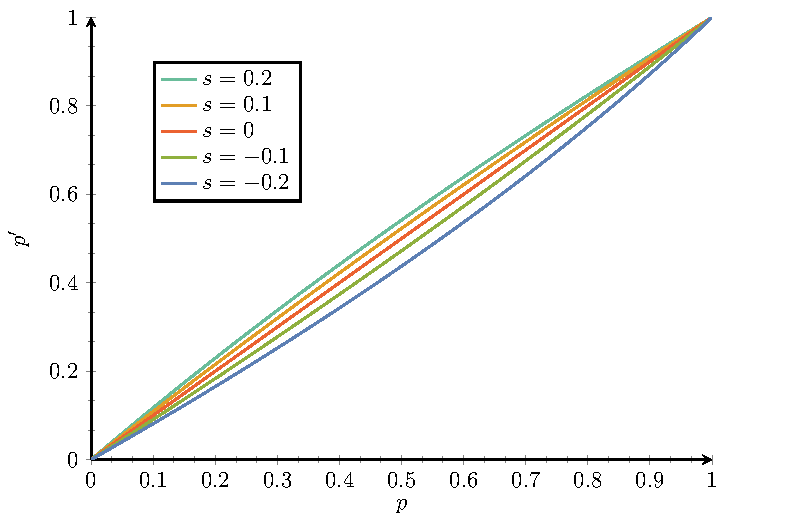
\includegraphics[width=0.8\textwidth, page=1] {figures.pdf}
	\end{center}
	\caption[Frequency of derived \gls{allele} after a generation]{Frequency of derived \gls{allele} after a generation. Positive selection coefficient ($s > 0$) result in increased derived \gls{allele} frequency at the next generation, which is intuitively expected. The effect is stronger when the derived \gls{allele} frequency is close to $0.5$, intuitively because the poll of both alleles must be sufficiently large such that they can be replaced. It is worth noting that even for strong selection coefficient ($s=0.2$), completely unrealistic in real population, the difference in frequency from one generation to the next is subtle.}
\end{figure}

The population is considered discrete and consists of a fixed number of \gls{diploid} individuals $\Ne \gg 1$, where the number of copies of the derived \gls{allele} $A$ present at the current generation is denoted $i$ and $p=i / 2\Ne $ 
The probability $\mathcal{P}_{ij}$, that there are $j$ copies of the derived \gls{allele} $A$ present at the next generation is given by the binomial distribution:
\begin{align}
\mathcal{P}_{ij} & = \binom{2 \Ne}{j} \left( p' \right)^j \left(1 - p' \right)^{2 \Ne -j} \\
				 & = \binom{2 \Ne}{j} \left( p\dfrac{1+s(1+p)}{1 + 2ps} \right)^j \left(1 - p\dfrac{1+s(1+p)}{1 + 2ps} \right)^{2 \Ne -j}
\end{align}

These {transition} probabilities define a discrete-space and discrete-time Markov process.
However, it has been shown to be extremely difficult to explicitly derive formulas for several quantities of evolutionary interest.
However, as the size of the population approaches infinity (i.e. $ \Ne \to \infty$), and assuming that the scaled selection pressure ($\Ne s $) remain constant, the discrete Markov process given above can be closely approximated by continuous-time and continuous-space diffusion process.\\

\subsection{Probability of fixation}
Starting from an initial frequency, the process eventually reach absorption, whether the derived \gls{allele} invade the population or dies out. 
Under the continuous-time and continuous-space diffusion process approximation, partial differential equations know as Kolmogorov backward equation allow to derive the probability of such events. 
If the selection coefficient is weak ($|s| \ll 1$), the probability of fixation ($P_{\mathrm{fix}}$) of a derived \gls{allele} with selection coefficient $s$ and initial frequency $p$ was derived by \citet{Kimura1962}:
\begin{align}
P_{\mathrm{fix}}(s, \Ne, p) & = \dfrac{1 - \e^{-4 \Ne p s }}{1 - \e^{-4 \Ne s}},\\
			     & = \dfrac{1 - \e^{- p S }}{1 - \e^{-S}},
\end{align}
where $S = 4 \Ne s$ is the scaled selection coefficient.
\begin{figure}[H]
	\begin{center}
		\includegraphics[width=0.8\textwidth, page=3] {figures.pdf}
	\end{center}
	\caption[Probability of fixation]{Probability of fixation. The selection coefficient of the derived \gls{allele} is scaled by population size $S=4 \Ne s$. In contrast to changes of frequency during a generation, the probability of fixation is sensitive to very weak selection coefficient ($|s| \ll 1$), as long as the scaled selection coefficient is not negligible ($|S| > 1$). Intuitively, selective effects are magnified by population size because the fixation is the inherently the resultant of the trajectory overall, integrating small effects throughout the lifespan of the \gls{allele}. }
\end{figure}

An interesting special case is obtained for a new mutation appearing in the population.
Because it is a single mutant the derived \gls{allele} initial frequency is $p = 1 / 2 \Ne$, and the probability of fixation ($P_{\mathrm{fix}}$) if given by:
\begin{align}
	P_{\mathrm{fix}}(s, \Ne) & = \dfrac{1 - \e^{-2 s}}{1 - \e^{-4 \Ne s}} \\
	 & \simeq  \dfrac{2 s }{1 - \e^{-4 \Ne s}}
\end{align}
The special case of a \gls{neutral} \gls{allele} can be obtained by taking the limit when $s$ goes to $0$.
\begin{align}
P_{\mathrm{fix}}(0, \Ne) & = \dfrac{1}{2 \Ne} \\
\end{align}
Altogether, the fixation probability of a selected \gls{allele} relative to a \gls{neutral} \gls{allele} is solely dependent on the scaled selection coefficient:
\begin{align}
R_{\mathrm{fix}}(S) & = \dfrac{P_{\mathrm{fix}}(s, \Ne)}{P_{\mathrm{fix}}(0, \Ne)} \\
& \simeq  \dfrac{S}{1 - \e^{-S}}
\end{align}
\begin{figure}[H]
	\begin{center}
		\includegraphics[width=0.8\textwidth, page=2] {figures.pdf}
	\end{center}
	\caption[Relative fixation probability]{Fixation probability of a selected \gls{allele} relative to a \gls{neutral} \gls{allele}.
	For a substantive negative scaled selection coefficient ($s \leq -1/\Ne$, red filled area), the probability of fixation is greatly reduced (by an exponential factor), and \gls{allele} can not likely reach fixation. On the other hand for a positive scaled selection coefficient ($s \geq 1 / \Ne$, green filled area), the ratio is approximately linear w.r.t $S$. In between, whenever the absolute value of is close to $1 / \Ne$ (yellow filled area), the \gls{allele} behave approximately neutrally.}
\end{figure}

\subsection{Site frequency spectrum}
The probability of fixation of an \gls{allele} can be empirically observable, and in the context of Wright-Fisher processes is related to selection and drift. 
However, this absorbing fate is not the sole characteristic of the process that relates empirical observable and parameter of evolution. 
Along the whole trajectory of an \gls{allele}, before fixation or extinction, the probability of this \gls{allele} to be at a certain frequency can be related to its selection coefficient and \gls{effective-population-size}.
More precisely, $g(x) \der x $ is the expected time for which the population frequency of derived \gls{allele} is in the range $(x, x+\der x)$ before eventual absorption, and can be derived using Kolmogorov forward equation:
\begin{align}
g(x, S) & = \dfrac{\left( 1 - \e^{- 2 s }\right) \left( 1 - \e^{-4 \Ne s(1-x)}\right)}{ s (1 - \e^{-4 \Ne s})x(1-x)} \\
& \approx \dfrac{2 \left[ 1 - \e^{-S(1-x)}\right]}{(1 - \e^{-S})x(1-x)} \label{eq:expected_time}
\end{align}

\begin{figure}[H]
	\begin{center}
		\includegraphics[width=0.8\textwidth, page=4] {figures.pdf}
	\end{center}
	\caption[Expected time at a derived frequency]{Expected time at a derived frequency. Allele with positive selection coefficient can be observed at high frequency, while alleles with negative selection coefficient are unlikely to be observed at high frequency.}
\end{figure}

This equation is solely valid for a gene with two alleles, a configuration which is scarcely observed in empirical data since more than two variants of a gene are usually present in the population.
However, its frequent to observe sites inside a gene sequence for which only two alleles are segregating.
This observation led to the development of modeling the Wright-Fisher process at multiple sites, by assuming that each site follow an independent process \citep{Sawyer1992}.
Strictly speaking, this model consider collection of independently evolving loci, meaning without linkage or equivalently considering free-recombination between sites.
Moreover, the collection is considered infinite whereas the total mutation rate across this infinite collection is considered finite.
Assumption of infinite sites is necessary to ensure that each mutation arise at a new site, with a Poisson distribution of rate $u$ per generation for the whole sequence.

From an empirical perceptive, for a sample of $n$ sequences taken in the population, the expected number of sites with $i$ (which ranges from $1$ to $n-1$) copies of the derived \gls{allele} is denoted $G(i, n)$. 
The collection of all $G(i, n)$ generate what is called a site frequency spectrum (\acrshort{SFS}), which can intuitively be interpreted as the discrete version the expected time at a derived frequency (equation \ref{eq:expected_time}), readily available from a sample of sequences from a population.
Given the scaled selection pressure ($S=4 \Ne s$), and the scaled mutation rate per generation for the whole sequence ($\theta = 4 \Ne u $), each entry of the \acrshort{SFS} is:
\begin{align}
	G(i, n) & = \int_{0}^{1}  2 \Ne u g(x) \binom{n}{i} x^{i} (1-x)^{n-i} \der x \\
	& = \theta \int_{0}^{1} \dfrac{1 - \e^{-S(1-x)}}{(1 - \e^{-S})x(1-x)} \binom{n}{i} x^{i} (1-x)^{n-i} \der x \\
	& =  \dfrac{\theta }{1 - \e^{-S}} \binom{n}{i} \int_{0}^{1} \left( 1 - \e^{-S(1-x)} \right) x^{i-1} (1-x)^{n-i-1} \der x 
\end{align}

This site frequency spectrum can be confronted to empirical data in order to estimate the selection coefficient of new mutations.
However, a single selection coefficient for all sites and all mutations is biologically not realistic, and selection coefficients are usually modeled as a continuous distribution, known as the distribution of fitness effects of mutations (\acrshort{DFE}).
Altogether, \acrshort{SFS} are empirically available and are function of the underlying \acrshort{DFE} which can thus be estimated \citep{eyre-walker_distribution_2006, eyre-walker_estimating_2009}.
In the context of protein coding \acrshort{DNA} sequences, synonymous sites (third position) not changing the amino-acid sequence are often assumed to be \gls{neutral}, and non-synonymous sites (first and second positions) are considered selected. 

\subsection{Wrightian fitness and selection coefficient}

Under the assumption that selection is weak $|s| \ll 1$, the selection coefficient is approximated by the difference in logarithm of Wrightian fitness between the mutant and resident \gls{allele}:
\begin{align}
s & = \dfrac{W_{B} - W_{A}}{W_{A}}, \\
& = \dfrac{W_{B}}{W_{A}} - 1, \\
& \simeq \ln\left( \dfrac{W_{B}}{W_{A}} \right), \\
& \simeq \ln(W_{B}) - \ln(W_{A}), \\
& \simeq f_{B} - f_{A}.
\end{align}
Where the logarithm of Wrightian fitness ($W$) is often referred as Malthusian fitness, or simply log-fitness ($f$).

\begin{table}[H]
	\begin{center}
		\begin{tabular}{|l|c|c|c|}
			\hline
			Parameter & Symbol & Range \\
			\hline
			Effective population size & $\Ne$ & $ [10^2, 10^6]$ \\
			Absolute Wrightian fitness & $W$ & $ \simeq 1 $ \\
			Relative fitness & $f=\ln(W)$ & $ \ll 1 $ \\
			Selection coefficient & $s$ & $ |s| \ll 1 $ \\
			Scaled selection coefficient & $S=4 \Ne s$ & Finite (negative or positive) \\
			Mutation rate per generation & $u$ & $[10^{-10}, 10^{-7}]$ per site \\
			Scaled mutation rate & $\theta = 4 \Ne u$ & $[10^{-8}, 10^{-1}]$ per site \\
			\hline
		\end{tabular}
	\end{center}
	\caption[Parameter of population-genetics]{Parameter of population-genetics}\label{table:params-popgen}
\end{table}


\section{Mutation-selection process}
The previous section recalled the Wright-Fisher process of evolution inside a population, relating selection and drift to the diversity of sequences, which empirically requires gene sequences for at least several individuals.
However, modeling sequence evolution between different species along lineages is a different endeavor, where species are often simplified with a single representative sequence, collapsing the intra-specific diversity of sequences.
Under this simplification, the inter-specific variability and evolutionary trajectory of sequences is described by the past history of point substitutions along lineages.
Such substitutions along lineages can nonetheless be decomposed into two mechanisms, their origination through mutation and their final fate of fixation, a modeling approach broadly known as origin-fixation \citep{McCandlish2014}.
Most importantly this decomposition of \gls{substitution} into mutation and fixation is able to conciliate population genetics and inter-specific protein evolution, where the \gls{substitution} history is parameterized by mutation, selection and drift.
Under the field of phylogenetic, the origin-fixation framework is more commonly known as mutation-selection, where fixation of an \gls{allele} encompass natural selection and origination correspond to mutation, a convention we will use hereafter.
However, a more general mathematical description of the mutation-selection framework recruiting tools from statistical physics can be found in \citet{Sella2005, Mustonen2009}.

Mutation-selection probabilistic models are usually Markovian with respect to time, such that the next \gls{substitution} event depends on the current representative sequence but not on earlier sequences visited in the history of a lineage.
This continuous-time Markovian process is valid if the mutation rate is sufficiently low, such that the event of a new mutations reaching fixation do so before the next one occurs. 
Since the rate of \gls{substitution} is equal to $u$ and that each \gls{allele} reaching fixation are segregating for an average of $4 \Ne$ generations \citep{Kimura1969}, this assumption is broadly applicable whenever the product of population size and mutation rate per generation for the sequence is lower than $1$ ($4 \Ne u \ll 1$).
More strictly, the model would require not only that new mutations reaching fixation do so before the next \gls{substitution} occurs, but before any mutation occurs, even the one that ultimately become extinct.
Since at each generation during the process an average of $2\Ne$ of mutations are produced, the point \gls{substitution} is valid under the condition that $8\Ne^2 u \ll 1$.
In practice, the assumptions that $4 \Ne u \ll 1$ is a sufficient condition for the process to be well approximated.
Throughout this development, it is important to note that $u$ is the mutation rate for the whole sequence under consideration.

For large sequence this approximation is not usually valid, and the sequence is then decomposed into each individual sites, forming a collection of independently evolving continuous-time Markov chains.
For such decomposition to be valid, these models have to assume free \gls{recombination} between sites.
In addition, these models assume by definition the absence of epistasis since the selection coefficient at each site must be independent of the alleles present at other sites. 
The mutation rate $u$ in the condition then refers to the mutation rate for each independent site, rather than the total mutation rate over the collection as a whole.
For example, \citet{Halpern1998} construct a model for the evolution of coding sequences where each \gls{codon} site is modeled as an independent \gls{mc}. 

\begin{figure}[thbp]
	\centering
	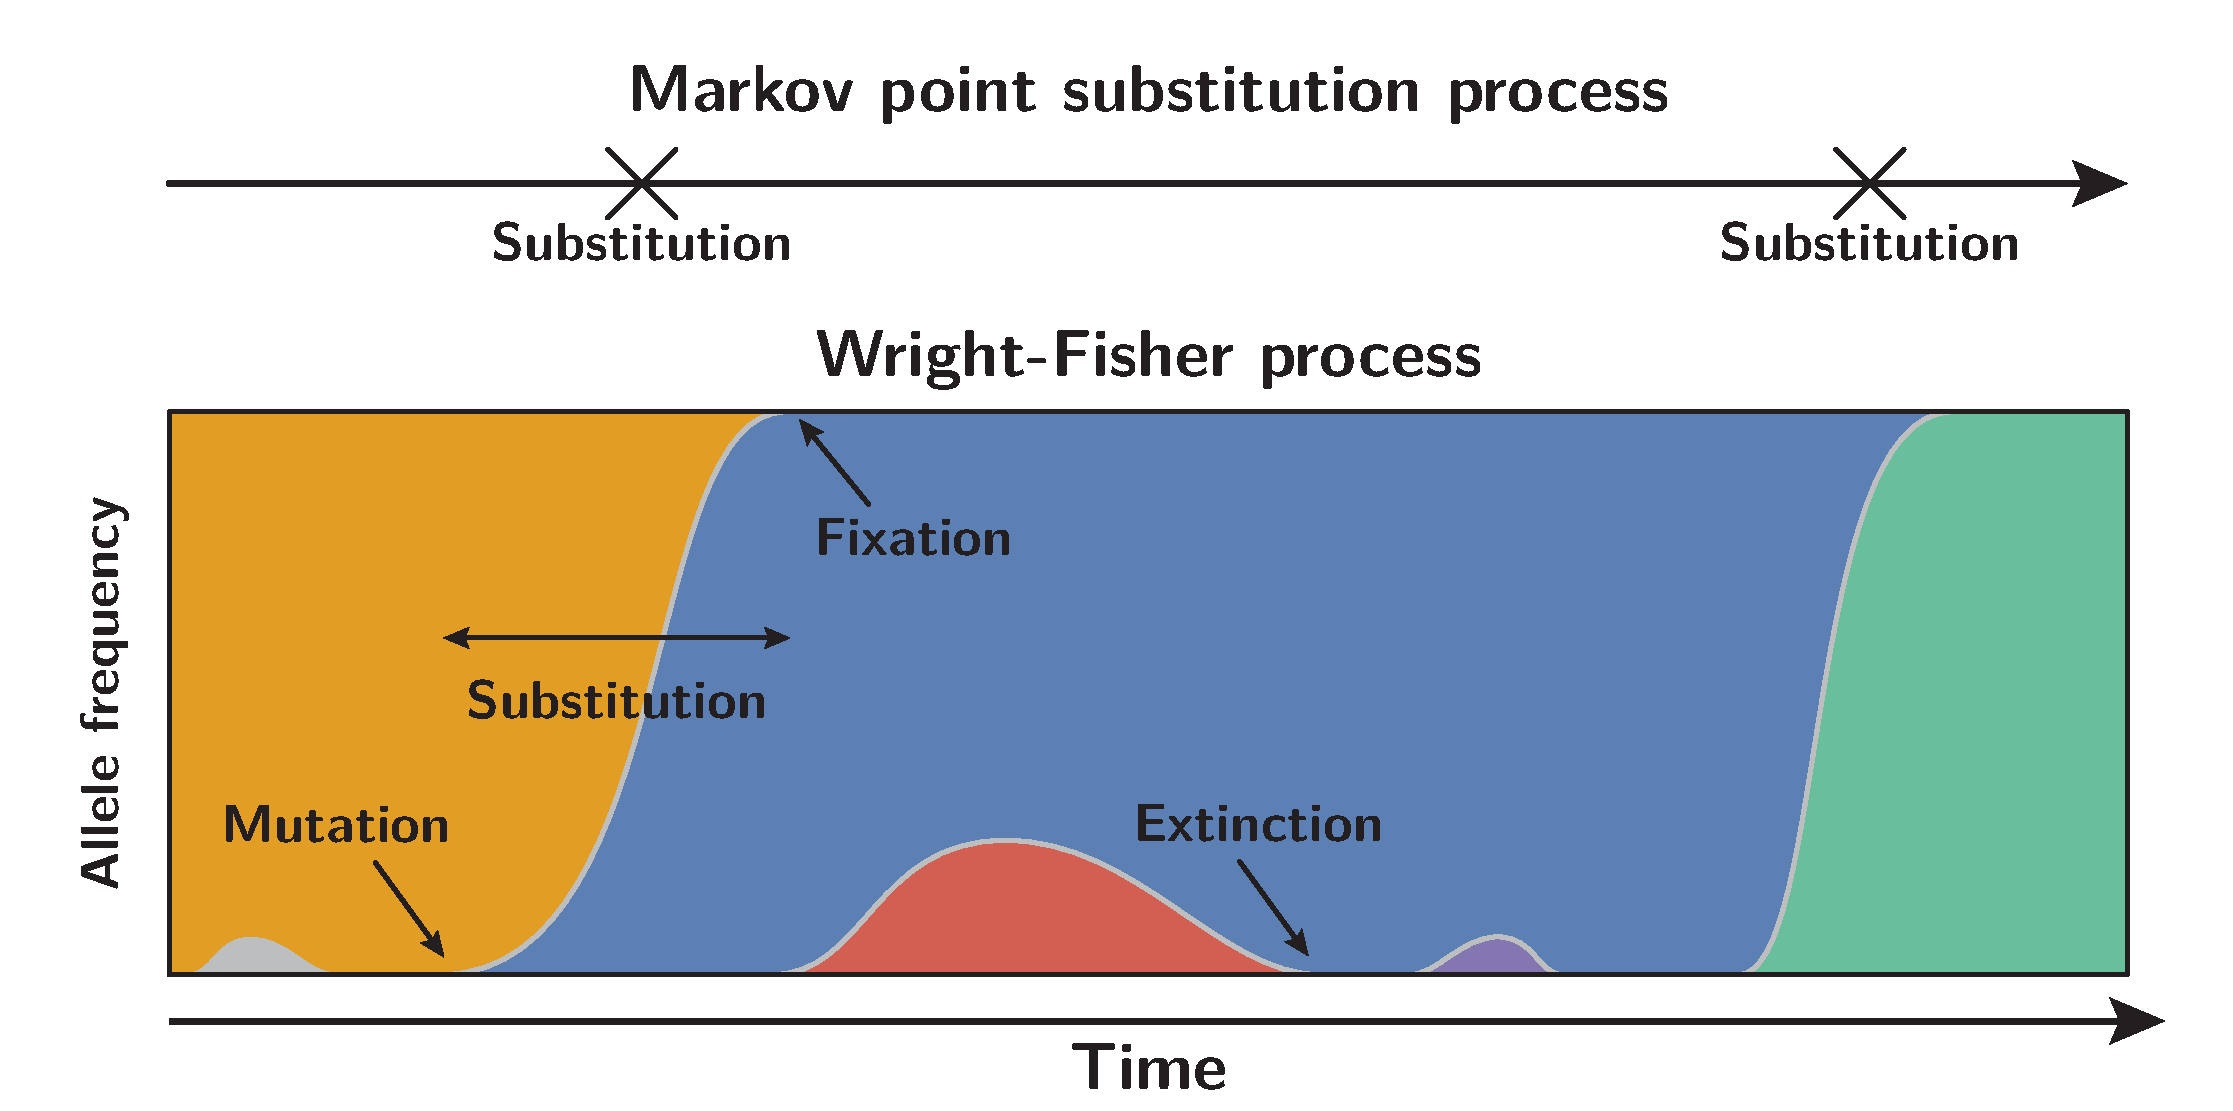
\includegraphics[width=0.6\textwidth]{figures/point-process.pdf}
	\caption[Mutation-selection point substitutions]{Mutation-selection point substitutions models. The trajectory of alleles inside a population is collapsed into a single point \gls{substitution} process. This approximation is valid under low mutation rate such that a mutation originate uniquely whenever the gene is monomorphic (with a single allele).}
\end{figure}

\subsection{Substitution rate}
The continuous-time Markov chain is defined by the instantaneous rate at which pair of states are transitioning.
Given the current state of the process is allele $A$, the rate of transition to other states can derived with population-genetics equations derived above.
At each generation, the expectation for the number of possible mutants is $2\Ne u$, and each of these mutant have a probability $P_{\mathrm{fix}}$ to result in a \gls{substitution}.
Altogether, the rate of \gls{substitution} from \gls{allele} $A$ to $B$, denoted $Q_{A \to B}$, is equal to the rate of mutation ($\mu_{A \to B}$) multiplied by the probability of fixation of the mutation $P_{\mathrm{fix}}(s_{A \to B}, \Ne)$ and scaled by the number of possible mutants at each generation ($2\Ne$):
\begin{align}
Q_{A \to B} & = 2 \Ne \mu_{A \to B}  P_{\mathrm{fix}}(s_{A \to B}, \Ne) \\
\end{align}
It is important to note that the \gls{substitution} rate and mutation rate are in the same unit, such that this equation is valid whether the rate is measured in unit of time or generation.
As a convention, mutation rate measured in unit of generation is denoted $u$, and denoted $\mu$ when measured in unit of time. As a consequence, $\submatrix$ is measured in unit of time in our equation.

In the case of \gls{neutral} mutations, the probability of fixation is independent of the original and target sequence, and equal $1/2 \Ne$. Finally the substitution rate $Q_{A \to B}$ simplifies to: 
\begin{align}
Q_{A \to B} & = 2 \Ne \mu_{A \to B}  P_{\mathrm{fix}}(0, \Ne) \\
Q_{A \to B} & = 2 \Ne \mu_{A \to B} \dfrac{1}{2\Ne} \\
Q_{A \to B} & =  \mu_{A \to B}
\end{align}
In the case of selected mutations, the probability of fixation depends on the difference of log-fitness ($f_i$ and $f_j$) between the two alleles:
\begin{align}
Q_{A \to B} & = 2 \Ne \mu_{A \to B} P_{\mathrm{fix}}(s_{A \to B}, \Ne) \\
			& = 2 \Ne \mu_{A \to B}  \dfrac{2(f_{B} - f_{A})}{1 - \e^{4\Ne(f_{A} - f_{B})} } \\
			& = \mu_{A \to B} \dfrac{F_{B} - F_{A}}{1 - \e^{F_{A} - F_{B}} }\text{, where } F = 4\Ne f \label{eq:sub-transion-rates}
\end{align}

It is important to note that if the difference of log-fitness tends to $0$, the \gls{substitution} rate equal the mutation rate:
\begin{align}
\lim_{|F_{B} - F_{A}| \to 0} Q_{A \to B} & = \mu_{A \to B}   \dfrac{F_{B} - F_{A}}{{1 - (1 + {F_{A} - F_{B}}) }} \nonumber \\
& =  \mu_{A \to B} 
\end{align}


Taken together, the transition rates which generates the \gls{substitution} history and ultimately the inter-specific diversity is parameterized solely by mutation, selection and drift.
Consequently, from a particular history of substitutions, one can theoretically estimate the parameter of selection, mutation and drift.

\subsection{Reversibility of the process}

The continuous-time Markov chain, defined by the transition rates between all possible alleles (equations \ref{eq:sub-transion-rates}) is irreducible, meaning it is always possible to go from any allele to any other possible allele, possibly in several substitutions.
Moreover, this substitution process is positive recurrent and aperiodic since any strictly positive transition rate is matched by a stricly positive transition for the reverse substitution.
More precisely, the substitution rate between two alleles is null only if the underlying mutation rate is null, in which case the transition rate for the reverse mutation is also null, hence the transition rate for the reverse substitution is also null.

Moreover, for an irreducible, positive recurrent and aperiodic continuous-time Markov chain, a necessary and sufficient condition to be reversible is given by Kolmogorov's criterion.
Kolmogorov's criterion implies that the product of transition rates through any closed loop is the same whenever the traversing is done forward or in reverse.
As an example for a Markov chain composed of $3$ alleles ($A$, $B$ and $C$) the transitions rate must satisfies the equality:
\begin{equation}
Q_{A \to B}Q_{B \to C}Q_{C \to A} = Q_{A \to C}Q_{C \to B}Q_{B \to A}
\end{equation}

\begin{figure}[htb!]
	\begin{center}
		\begin{tikzpicture}[->,>=stealth',auto,node distance=1.2cm and 1.6cm,semithick]
		\tikzstyle{every state}=[]
		
		\node[] (0) {};
		\node[state] (A) [above=of 0] {$A$};
		\node[state] (B) [below left=of 0] {$B$};
		\node[state] (C) [below right=of 0] {$C$};
		
		\path[->]
		(A) edge [BLUE,bend right=45] node [left] {$Q_{A \to B}$} (B)
		(B) edge [BLUE,bend right=45] node [below] {$Q_{B \to C}$} (C)
		(C) edge [BLUE,bend right=45] node [right] {$Q_{C \to A}$} (A)
		(B) edge [RED,bend right=15] node [left] {$Q_{B \to A}$} (A)
		(C) edge [RED,bend right=15] node [below] {$Q_{C \to B}$} (B)
		(A) edge [RED,bend right=15] node [right] {$Q_{A \to C}$} (C);
		\end{tikzpicture}
	\end{center}
	\caption[Kolmogorov's criterion]{The continuous-time Markov chain is reversible if the process fulfills Kolmogorov's criterion, such that the product of transition rate for a closed loop is equal whether traversed in one sens (blue arrows) or the other (red arrows).}
	\label{fig:reversible-circuit}%
\end{figure}

From transition rates of the substitution process (\ref{eq:sub-transion-rates}), Kolmogorov's criterion can be derived as:
\begin{align}
\dfrac{Q_{A \to B}Q_{B \to C}Q_{C \to A}}{Q_{A \to C}Q_{C \to B}Q_{B \to A}}
={}& \dfrac{\mu_{A \to B}\mu_{B \to C}\mu_{C \to A}}{\mu_{A \to C}\mu_{C \to B}\mu_{B \to A}}
	 \times \dfrac{(F_{B} - F_{A})(F_{C} - F_{B})(F_{A} - F_{C})}{(F_{C} - F_{A})(F_{B} - F_{C})(F_{A} - F_{B})} \notag \\
	 &\ \times \dfrac{( 1 - \e^{F_{A} - F_{C}} )( 1 - \e^{F_{C} - F_{B}} )( 1 - \e^{F_{B} - F_{A}} )}{( 1 - \e^{F_{A} - F_{B}} )( 1 - \e^{F_{B} - F_{C}} )( 1 - \e^{F_{C} - F_{A}} )}, \\
={}& - \dfrac{\mu_{A \to B}\mu_{B \to C}\mu_{C \to A}}{\mu_{A \to C}\mu_{C \to B}\mu_{B \to A}} \notag \\
&\ \times \dfrac{\e^{F_{A}}( \e^{-F_{A}} - \e^{ - F_{C}} )\e^{F_{C}}( \e^{-F_{C}} - \e^{ - F_{B}} )\e^{F_{B}}( \e^{-F_{B}} - \e^{ - F_{A}} )}{\e^{F_{A}}( \e^{-F_{A}} - \e^{ - F_{B}} )\e^{F_{B}}( \e^{-F_{B}} - \e^{ - F_{C}} )\e^{F_{C}}( \e^{-F_{C}} - \e^{ - F_{A}} )}, \\
={}& \dfrac{\mu_{A \to B}\mu_{B \to C}\mu_{C \to A}}{\mu_{A \to C}\mu_{C \to B}\mu_{B \to A}}.
\end{align}
As a result, Kolmogorov's criterion for the substitution process is satisfied only if the mutation process is also reversible, in which case Kolmogorov's criterion is also fulfilled:
\begin{equation}
\mu_{A \to B}\mu_{B \to C}\mu_{C \to A}=\mu_{A \to C}\mu_{C \to B}\mu_{B \to A}.
\end{equation}
This example can be generalized for any close loop, such that the reversibility of the substitution process is conditioned on the reversibility of the underlying mutation process, which is often assumed.

\subsection{Stationary distribution}

A realization of the \gls{mc} for a long period of time results in a given proportion of the time for which the process is fixed for a specific allele, where this proportion depends of the allele fitnesses, the mutational process and $\Ne$.
Because the continuous-time \gls{mc} is irreducible, positive recurrent and aperiodic, it has a unique stationary distribution $\bm{\pi}$ where $\pi_{A}$ corresponds to the proportion of time spent in allele $A$ after the Markov chain has run for an infinite amount of time. 

Moreover, under the condition that the \gls{mc} is time-reversible, the detailed balanced for the stationary distribution is satisfied:
\begin{align}
\dfrac{\pi_{A}}{\pi_{B}} & = \dfrac{Q_{B \to A}}{Q_{A \to B}} \\
& = \dfrac{\mu_{B \to A}}{\mu_{A \to B}}  \dfrac{F_{A}-F_{B}}{ 1 - \e^{F_{B}-F_{B}}}  \dfrac{1 - \e^{F_{A} - F_{B}} }{F_{B} - F_{A}}\\
& = - \dfrac{\mu_{B \to A}}{\mu_{A \to B}}  \dfrac{ \e^{F_{A}}(\e^{-F_{A}} - \e^{- F_{B}}) }{ \e^{F_{B}}(\e^{-F_{B}} - \e^{- F_{A}})}  \\
& = \dfrac{\mu_{B \to A}}{\mu_{A \to B}} \dfrac{\e^{F_{A}}}{\e^{F_{B}}} \\
\end{align}
Under the assumption that the mutational process is also reversible, the detailed balanced for the stationary distribution of the mutation process ($\backref{\sigma}$) is satisfied:
\begin{align}
\dfrac{\mu_{B \to A}}{\mu_{A \to B}} & = \dfrac{\sigma_{A}}{\sigma_{B}} 
\end{align}
Altogether, the probability $\pi_{A}$ to find the population in allele $A$ is proportional to a function (also called a Boltzmann factor) that depends only on the fitness of allele $A$, the population size, and details of the mutation process \citep{Sella2005,Mustonen2005}:
\begin{align}
\dfrac{\pi_{A}}{\pi_{B}} & = \dfrac{\sigma_{A}\e^{F_{A}}}{\sigma_{B}\e^{F_{B}}} \text{ and } \sum_{A}\pi_{A} = 1, \\ 
\iff \pi_{A} & = \dfrac{\sigma_{A}\e^{F_{A}}}{\sum_{B} \sigma_{B}\e^{F_{B}} },
\end{align}
where the denominator is a normalizing constant such that the sum of probabilities equal to $1$.
In analogy to thermodynamic systems, the evolutionary system reaches thus a Boltzmann-like distribution with $\Ne^{-1}$ playing the role of evolutionary temperature, and the log-fitness $f$ the role of energy\footnote{At high mutation rates, the quasi-species theory provides another analogy with statistical mechanics, in which the mutation rate plays the role of temperature instead of genetic drift.}.

\subsection{Relative {substitution} rate} 

Probabilities of the stationary distribution allows to calculate all observable quantities of interest, such as mean fitness and mean \gls{substitution} rate, using standard probability theory.
One quantity of interest is the \gls{substitution} rate of selected mutations relative to that of \gls{neutral} mutations, called $\omega$.
From its definition, $\omega=1$ for genes or sites under \gls{neutral} evolution.
Most importantly, departure from $1$ would be interpreted as a signature of selection on sequences. 
First, $\omega>1$ is interpreted as a signal of adaptive recurrent evolution, where selection coefficient are on average positive.
On the other hand, $\omega<1$ is a signal of underlying purifying selection, such that the sequence is constrained and mutations proposed have on average a negatively selection coefficient.
Together, in the case of a mutation-selection point \gls{substitution} process, $\omega$ is defined as:
\begin{equation}
\omega = \dfrac{ \sum_{A} \pi_{A} \sum_{B} Q_{A \to B}}{\sum_{A} \pi_{A}  \sum_{B} \mu_{A \to B}},
\end{equation}
It worth noting that under the assumption of a static fitness landscape, a mutation-selection point \gls{substitution} process will result in $\omega \leq 1$. 

\begin{table}[H]
	\begin{center}
		\begin{tabular}{|l|c|c|c|}
			\hline
			Parameter & Symbol & Range \\
			\hline
			Scaled fitness & $F=4 \Ne f$ & finite, positive or negative \\
			Mutation rate per time & $\mu$ & $[10^{-11}, 10^{-8}]$ per site per year \\
			Substitution rate per time & $Q$ & $[10^{-11}, 10^{-8}]$ per site per year \\
			Equilibrium frequency & $\Pi$ & $[0, 1]$ \\
			Equilibrium frequency under mutation & $\sigma$ & $[0, 1]$ \\
			Relative \gls{substitution} rate & $\omega$ & $[0, 1]$ for purifying selection\\
			\hline
		\end{tabular}
	\end{center}
	\caption[Parameter of mutation-selection processes]{Parameter of mutation-selection processes}\label{table:params-mutsel}
\end{table}

\section{Mutation-selection analogy}

This section develops reflections on apparent similarities and analogies between the mutation-selection process and other processes present in a variety of scientific fields outside of evolutionary biology, displaying the same underlying mechanism and emerging properties, though with different name and aspiration.
This effort is made in the aim of giving another view of the mutation-selection process, such as to better appreciate and conceptualize its assumptions, its limits, and the respective role of the different components. 
Such attempts requires to boil down the mutation-selection mechanism into its core components, while at the same time rephrasing the description using lexicography outside of population-genetic such as to open new perceiving angles.

At the bottom, mutation is a process creating diversity, changing and moving the current viable state to a novel and unknown position, fundamentally allowing exploration of the state space.
On the other hand, selection is the criteria on which a new state is deemed a disrupting innovation or a nonviable alteration, and allow to determine which changes to exploit and which to filter out and discard based on its fitness.
Fundamentally, reducing the diversity created by the mutation process is the very essence of selection.
Finally, drift arbitrate between the creation and reduction of the two processes, it dictates how much exploration of novelty is permitted, and conversely how much exploitation of only the fittest states is granted.

I argue that this creation and reduction process is found at the core of several research disciplines, while the link between them is scarcely made \citep{Baeck1994, Eiben1998}. 

\subsection{Metropolis-Hasting sampling}
Obtaining a sequence of random samples from a probability distribution can be difficult, especially when the number of dimensions is high.
However, the Metropolis-Hasting procedure based on a Monte Carlo \gls{mc} can sample from any probability distribution, provided that we know how to compute the probability density, or even less restrictively any function proportional to the density \citep{Hastings1970}.
This stochastic procedure which is based on three steps bears many similarities with the mutation-selection process:
\begin{itemize}
	\item Generate a stochastic candidate from the current state, analogous to the mutation.
	\item Calculate the acceptance ratio as the ratio of the two densities, analogous to the selection coefficient of the mutated state.
	\item Stochastic acceptance or rejection based on the acceptance ratio, a process analogous to drift. 
\end{itemize}
Inherently, Metropolis-Hasting procedure is based on creating and subsequently reducing diversity, which allows to obtain a random sequence of samples from any distribution with a straightforward recipe, and is a critical tools in statistic and statistical physics.

\subsection{The exploration-exploitation dilemma}
Many mathematical, engineering and day-life problems are not about sampling a state space, but rather finding the optimal and best state given a criteria or a function to maximize.
Naturally, we would prefer deterministic (strictly reproducible) rather than stochastic optimizing strategies to search for an optimal state.
Unfortunately, whenever the state space is too large, often due to the curse of dimensionality, a greedy or heuristic search of an optimal state can performs atrociously \citep{Bellman1966}.
In high dimensional space, stochastic optimization tools have been deemed very valuable, such as stochastic gradient decent or so called evolutionary algorithm \citep{Russell2010,Vikhar2017}.
Inherently, they are based on two processes, one is stochastically creating diversity and exploring the state space, while the other is filtering the explored states and thus reducing the diversity.

In the constrained case of a finite number of time or attempts to find the best outcome overall, the problem is best described by the multi-armed bandit problem. The name comes from imagining a gambler at a row of slot machines (sometimes known as one-armed bandits), where each slot machine provides a random reward from a probability distribution specific to that machine. The player has to decide which machines to play, how many times to play each machine and in which order to play them, and whether to continue with the current machine or try a different machine, such as to maximize the sum of rewards earned through a sequence of trials.
The gambler faces a dilemma at each trial, either reducing his regret by exploiting the best arm, or gaining information through exploration of other arms.
The best strategy to solved this dilemma can be mathematically derived in numerous cases, and encompass a mixing strategies with a defined ratio of exploration and exploitation \citep{Auer2002,Kocsis2006,Furnkranz2006}.
This problem is far from be only theoretical, and has be used to explain a multitude of phenomena, such as the movement of animals in novel landscapes, the most efficient resource allocation for a start-up company, the effects of age on knowledge acquisition in humans, and in search of the most efficient treatment in clinical trials (hence the name a clinical arm) \citep{Berger-Tal2014, March}. 
An other application of the exploration-exploitation dilemma is AlphaGo, the first computational program mastering the board game go at the professional 9-dan level in 2017, and out-compete Ke Jie, the world n°1 ranked player at the time \citep{Silver2017, Silver2018}.
AlphaGo has often been publicized and hyped in various media outlets that this feat was possible due to machine learning, more specifically due to convolutionnal neural networks.
However, it is more scarcely mentioned that AlphaGo neural network is combined with an exploration-exploitation algorithm, or more specifically Monte Carlo tree search. 
In practice, the convolutionnal neural network is used as a criteria to measure the advantage of a board configuration\footnote{Convolutionnal neural networks also use a stochastic gradient descend to reach convergence, inherently leveraging stochastic exploration and exploitation procedure to optimize the parameters of the neural network.}, but the different moves and path probed and trimmed is done via an exploration-exploitation procedure. 


Altogether, exploration and exploitation, creation and reduction, mutation and selection, are different names that encompass the inherently same process efficiently sampling and optimizing whenever the state is too large to be traversed.
I argue that scientific research endeavor is also a exploration-exploitation dilemma, which is arguably externally pressured to pursue exploitation, through funding of impactful research and a \textit{publish-or-perish} systemic culture in early career stage.

% As a side note, it appears that drift and selection are actually confounded, they are both on the side of exploitation, not on exploration.
As a side note, mutation is a necessary process of evolution, while sexe is not mandatory but increase the diversity of genomes between generations.
Arguably, studying evolution while disregarding mutation is a sufficient approximation whenever mutation rate and number of generations is low, which is developed thoroughly through the whole field of quantitative genetics.
Sex and mutation are both generating new states and are part of the more general exploration facet.
This explains why sex is favored in fluctuating environments.

I argue that evolutionary biologists, studying and leveraging the pervasive process of mutation and selection, can gain knowledge by recruiting insight and developments from other fields, much like there as been many crossover between economics and evolution in the context of game theory.\footnote{Game theory had originally been developed to model economic actors behavior and strategies \citep{VonNeumann1947}, while latter being emerging as the framework of evolutionary dynamics, which explains the emergence of altruistic behaviours in Darwinian evolution \citep{Smith1973, Smith1982, Nowak2006}.}.

As an example of such insight from exploration-exploitation dilemma is on the understanding of relationship between mutation rate and chromosome size.
It has been observed that organism with a low mutation rate (per site per generation) tend also to have a long chromosome size, such that the product of genome size and mutation rate is constant \cite{Drake1991}.
An explanation for this pervasive negative correlation between mutation rate and genome size invoke the drift barrier hypothesis, where the correlation is inherently due to an underlying changes of genetic drift \citep{Lynch2016a}.
The drift barrier hypothesis posits the selection operates to minimize the mutation rate, with the efficiency of such improvement eventually being overcome by random genetic drift, such that population with higher population size have smaller mutation rate. 
On the other hand, higher population size induces stronger purifying selection which reduce genome size by expelling transposable elements.
Altogether, both high mutation rate and smaller genome are consequences of higher population size.
An alternative explanation for the negative correlation between mutation rate and genome size is that for each new generation, the genetic diversity of offsprings must balance the trade-off between exploration of new genotype and the reliable transmission of the current one.
The genetic difference between parents and offsprings is the product of mutation rate and genome size, such that individuals whom are not robust enough undergo deleterious mutations and disappear, whereas individuals whose genotypes are not variable enough are outcompeted by those that were able to discover innovations \citep{Knibbe2007, Beslon2010, Hindre2012, Batut2014, Biller2016}.



\chapter{Selection in protein coding {DNA} sequences}
{
	\hypersetup{linkcolor=GREYDARK}
	\minitoc
}
\label{sec:selection}

Evolutionary trajectory of sequences depends on the forces of mutation, selection and drift, which acts conjointly such that each one of them must be well studied and understood.
However, the previous chapter remained so far elusive on selection, and did not yet question what determines the strength of selection.
More precisely, molecular evolution requires either a given selection coefficient associated to mutation, or that the fitness of each particular sequence to be defined.
In other word, the relationship between sequence and fitness must be elucidated, which is the focus of the present chapter in the special case of protein coding \acrshort{DNA} sequence.
It will seek to clarify the relationship between protein sequence, protein thermodynamic, protein function, and organismal fitness, such as to derive the selective pressures shaping proteins coding \acrshort{DNA} sequences.
It is also important to emphasize whether they are general principles, or do this relationship between sequence and fitness depends on the specific protein, organism, and environment.
To this aims, this chapter will first present the genetic code and broad chemical properties of amino-acids, as well as how \glspl{codon} and amino-acids are connected by single nucleotide mutations in section \ref{sec-intro:genetic-code}.
Subsequently, physico-chemical constrains of proteins and thermodynamics models of protein selection are related to empirical results \ref{sec-intro:physic-protein}.
Finally, phylogenetic models can quantify the strength of selection acting on proteins trough an aggregate parameter (called $\dnds$), \ref{sec-intro:rate-evolution}.
More precisely, empirical \acrshort{DNA} alignment provides insight on the variation of selective strength between different orthologous genes, between sites of the same protein, or between branches of the phylogenetic tree.

\section{Protein coding {DNA} sequences}
\label{sec-intro:genetic-code}
Proteins have a variety of molecular and cellular roles, they are the enzymes that catalyses chemical bonds, they regulate cell processes and control their rates, they carry signals within the cell and across membranes, they bind and transport small molecules, they form cellular structures, and so on.
This variety of roles is accomplished by a variety of three-dimensional shapes.
A protein's three-dimensional shape is in turn determined by the linear one-dimensional sequence of amino-acids, with their size ranging from fewer than $20$ to more than $5000$ amino acids, with an average of about 350 amino-acids.
Just as \acrshort{DNA} is oriented because of the asymetry of nucleotides, proteins are oriented due to asymetry of amino-acids, one end is called \gls{N-ter} and the other end C-terminus, and each amino-acid will interact with the other amino-acids in its spatial vicinity. 

Although each of the 20 different amino acids has unique biochemical properties, they can be classified broadly into four categories determining their solubility and acidity (classification is given in table \ref{table:genetic_code}).
Charged amino-acids can be either basic (positively charged) or acidic (negatively charged).
On the other hand, non charged amino-acids can however be polar due to an uneven charge distribution, such that they can form hydrogen bonds with water.
Consequently, polar amino acids are called hydrophilic, and are often found on the outer surface of folded proteins.
Also, non charged amino-acids can have a uniform charge distribution, and do not form hydrogen bonds with water.
Reciprocally, these non polar amino-acids are called hydrophobic and tend to be found in the core of folded proteins.

\subsection{Genetic code}

Because the $20$ letter alphabet of proteins is different to the $4$ letter alphabet of nucleic acid (DNA and RNA), there is not a one-to-one correspondence between the two alphabets.
Instead, amino acids are encoded by \glspl{codon}, a consecutive sequences of 3 nucleotides, yielding $4^3=64$ possible permutations, more than sufficient to encode the 20 different amino acids.
Moreover, three stop \glspl{codon} signals termination of the protein, such that 61 of the 64 \glspl{codon} are used to encode amino acids.
Since there are 61 coding \glspl{codon} and only 20 amino acids, there is a necessary redundancy in the code.
Thus, amino-acids are encoded by synonymous \glspl{codon}, which are interchangeable in the sense of producing the same amino acid, with the notable exception of methionine and tryptophan.
Altogether, the \acrshort{DNA} genetic code translating \gls{codon} to amino-acids, which is used almost universally by all organisms is given in table \ref{table:genetic_code}.

\begin{table}[H]
	\centering
	\noindent\adjustbox{max width=\textwidth}{%
		\begin{tabular}{|c||l|c|l|c|l|c|l|c||c|}
			\hhline{|-||-|-|-|-|-|-|-|-||-|}
			& \multicolumn{2}{c|}{\textbf{T}} & \multicolumn{2}{c|}{\textbf{C}} & \multicolumn{2}{c|}{\textbf{A}} & \multicolumn{2}{c||}{\textbf{G}} & \\
			\hhline{=#========#=}
			\multirow{4}{*}{\textbf{T}} & TTT & \cellcolor{Nonpolar} & TCT & \cellcolor{Polar} & TAT & \cellcolor{Polar} & TGT & \cellcolor{Polar} & \textbf{T} \\
			\cline{2-2} \cline{4-4} \cline{6-6} \cline{8-8} \cline{10-10}
			& TTC & \cellcolor{Nonpolar} \multirow{-2}{*}{Phenylalanine (Phe/P)} & TCC & \cellcolor{Polar} & TAC & \cellcolor{Polar} \multirow{-2}{*}{Tyrosine (Tyr/Y)} & TGC & \cellcolor{Polar} \multirow{-2}{*}{Cysteine (Cys/C)} & \textbf{C} \\
			\hhline{|~||-|-|-|>{\arrayrulecolor{Polar}}->{\arrayrulecolor{black}}|-|-|-|-||-|}
			& TTA & \cellcolor{Nonpolar} & TCA & \cellcolor{Polar} & TAA & \cellcolor{Stop} Stop (Ochre) & TGA & \cellcolor{Stop} Stop (Opal) & \textbf{A} \\
			\hhline{|~||-|>{\arrayrulecolor{Nonpolar}}->{\arrayrulecolor{black}}|-|>{\arrayrulecolor{Polar}}->{\arrayrulecolor{black}}|-|-|-|-||-|}
			& TTG & \cellcolor{Nonpolar} & TCG & \cellcolor{Polar} \multirow{-4}{*}{Serine (Ser/S)} & TAG & \cellcolor{Stop} Stop (Amber) & TGG & \cellcolor{Nonpolar} Tryptophan (Trp/W) & \textbf{G} \\
			\hhline{|-||-|>{\arrayrulecolor{Nonpolar}}->{\arrayrulecolor{black}}|-|-|-|-|-|-||-|}
			\multirow{4}{*}{\textbf{C}} & CTT & \cellcolor{Nonpolar} & CCT & \cellcolor{Nonpolar} & CAT & \cellcolor{Basic} & CGT & \cellcolor{Basic} & \textbf{T} \\
			\cline{2-2} \cline{4-4} \cline{6-6} \cline{8-8} \cline{10-10}
			& CTC & \cellcolor{Nonpolar} & CCC & \cellcolor{Nonpolar} & CAC & \cellcolor{Basic} \multirow{-2}{*}{Histidine (His/H)} & CGC & \cellcolor{Basic} & \textbf{C} \\
			\hhline{|~||-|>{\arrayrulecolor{Nonpolar}}->{\arrayrulecolor{black}}|-|>{\arrayrulecolor{Nonpolar}}->{\arrayrulecolor{black}}|-|-|-|>{\arrayrulecolor{Basic}}->{\arrayrulecolor{black}}||-|}
			& CTA & \cellcolor{Nonpolar} & CCA & \cellcolor{Nonpolar} & CAA & \cellcolor{Polar} & CGA & \cellcolor{Basic} & \textbf{A} \\
			\cline{2-2} \cline{4-4} \cline{6-6} \cline{8-8} \cline{10-10}
			& CTG & \cellcolor{Nonpolar} \multirow{-6}{*}{Leucine (Leu/L)} & CCG & \cellcolor{Nonpolar} \multirow{-4}{*}{Proline (Pro/P)} & CAG & \cellcolor{Polar} \multirow{-2}{*}{Glutamine (Gln/Q)} & CGG & \cellcolor{Basic} \multirow{-4}{*}{Arginine (Arg/R)} & \textbf{G} \\
			\hhline{|-||-|-|-|-|-|-|-|-||-|}
			\multirow{4}{*}{\textbf{A}} & ATT & \cellcolor{Nonpolar} & ACT & \cellcolor{Polar} & AAT & \cellcolor{Polar} & AGT & \cellcolor{Polar} & \textbf{T} \\
			\cline{2-2} \cline{4-4}\cline{6-6} \cline{8-8} \cline{10-10}
			& ATC & \cellcolor{Nonpolar} & ACC & \cellcolor{Polar} & AAC & \cellcolor{Polar} \multirow{-2}{*}{Asparagine (Asn/N)} & AGC & \cellcolor{Polar} \multirow{-2}{*}{Serine (Ser/S)} & \textbf{C} \\
			\hhline{|~||-|>{\arrayrulecolor{Nonpolar}}->{\arrayrulecolor{black}}|-|>{\arrayrulecolor{Polar}}->{\arrayrulecolor{black}}|-|-|-|-||-|}
			& ATA & \cellcolor{Nonpolar} \multirow{-3}{*}{Isoleucine (Ile/I)} & ACA & \cellcolor{Polar} & AAA & \cellcolor{Basic} & AGA & \cellcolor{Basic} & \textbf{A} \\
			\hhline{|~||-|-|-|>{\arrayrulecolor{Polar}}->{\arrayrulecolor{black}}|-|>{\arrayrulecolor{Basic}}->{\arrayrulecolor{black}}|-|>{\arrayrulecolor{Basic}}->{\arrayrulecolor{black}}||-|}
			& ATG & \cellcolor{Nonpolar} Methionine (Met/M) & ACG & \cellcolor{Polar} \multirow{-4}{*}{Threonine (Thr/T)} & AAG & \cellcolor{Basic} \multirow{-2}{*}{Lysine (Lys/K)} & AGG & \cellcolor{Basic} \multirow{-2}{*}{Arginine (Arg/R)} & \textbf{G} \\
			\hhline{|-||-|-|-|-|-|-|-|-||-|}
			\multirow{4}{*}{\textbf{G}} & GTT & \cellcolor{Nonpolar} & GCT & \cellcolor{Nonpolar} & GAT & \cellcolor{Acidic} & GGT & \cellcolor{Nonpolar} & \textbf{T} \\
			\cline{2-2} \cline{4-4} \cline{6-6} \cline{8-8} \cline{10-10}
			& GTC & \cellcolor{Nonpolar} & GCC & \cellcolor{Nonpolar} & GAC & \cellcolor{Acidic} \multirow{-2}{*}{Aspartic acid (Asp/D)} & GGC & \cellcolor{Nonpolar} & \textbf{C} \\
			\hhline{|~||-|>{\arrayrulecolor{Nonpolar}}->{\arrayrulecolor{black}}|-|>{\arrayrulecolor{Nonpolar}}->{\arrayrulecolor{black}}|-|-|-|>{\arrayrulecolor{Nonpolar}}->{\arrayrulecolor{black}}||-|}
			& GTA & \cellcolor{Nonpolar} & GCA & \cellcolor{Nonpolar} & GAA & \cellcolor{Acidic} & GGA & \cellcolor{Nonpolar} & \textbf{A} \\
			\cline{2-2} \cline{4-4} \cline{6-6} \cline{8-8} \cline{10-10}
			& GTG & \cellcolor{Nonpolar} \multirow{-4}{*}{Valine (Val/V)} & GCG & \cellcolor{Nonpolar} \multirow{-4}{*}{Alanine (Ala/A)} & GAG & \cellcolor{Acidic} \multirow{-2}{*}{Glutamic acid (Glu/E)} & GGG & \cellcolor{Nonpolar} \multirow{-4}{*}{Glycine (Gly/G)} & \textbf{G} \\
			\hhline{|-||-|-|-|-|-|-|-|-||-|}
	\end{tabular}}
	\caption[The Genetic Code]{
		The genetic code \acrshort{DNA} table translating \glspl{codon} into amino-acids.
		Amino-acids are represent into $4$ categories based on the electrochemical properties.
		Non-polar in yellow (\textcolor{Nonpolar}{\ding{110}}), polar in green (\textcolor{Polar}{\ding{110}}), basic in blue (\textcolor{Basic}{\ding{110}}) and finally acidic in red (\textcolor{Acidic}{\ding{110}}).
		Stop \glspl{codon} are represented in black (\textcolor{Stop}{\ding{110}}).
		The synonymous \glspl{codon} encoding for the same amino-acid are usually different by their third \gls{codon} position, the wooble base.
	}
	\label{table:genetic_code}
\end{table}

Biochemical translation from \gls{codon} to amino-acid mechanistically emanates from transfer \acrshort{RNA} (\acrshort{tRNA}).
More precisely, \glspl{codon} binds to \acrshort{tRNA} via an anticodon, three consecutive bases that are complementary and antiparallel to the associated \gls{codon}.
On the other end, \acrshort{tRNA} structure complexes uniquely with one the $20$ amino acid, where the catalytic reaction is performed by aminoacyl-tRNA synthetase~\citep{Rich1976}.
As a result, \acrshort{tRNA} genes along with aminoacyl-tRNA synthetase genes constitute the machinery necessary for translating \glspl{codon} into amino-acids.
However, there is not a one-to-one correspondence between the $61$ \glspl{codon} and \acrshort{tRNA} genes.
First, the set of unique sequence of anticodon found in tRNAs genes is actually lower than $61$, and depends on the species but varies from $41$ to $55$~\citep{Goodenbour2006}.
This subset of anticodon sequences necessary to binds all $61$ \glspl{codon} is due to non canonical base pairing\footnote{Canonical base pairing are A-U and G-C, where thymin (T) is replaced by uracil (U) in RNA}.
More precisely, the first two positions in the \gls{codon} bond strongly to the anticodon of the \acrshort{tRNA} (second and third positions), while the third base of the \gls{codon} can be subject to non standard pairing with the first base of the anticodon.
If the anticodon contains a guanine at first position, \glspl{codon} with either U or C at the third position can bounds to this anticodon, and this phenomenon explains why there is not any non-synonymous {transition} from only U to C at third position, and why synonymous \glspl{codon} usually end with T or C.
Also, if the anticodon contains an Inosine at first position, \glspl{codon} with either C, U or A at the third position can bounds to this anticodon, such that for example Leucine encoded by three \gls{codon} (AUU, AUC, AUA) can be bounded by the unique anticodon IAU.
Altogether, non-standard pairing explains why the number of unique anticodons is lower than the number of possible \glspl{codon}, and also explains some part of the structure of the genetic code.

Secondly, \acrshort{tRNA} genes with the same amino-acid binding site and anticodon, which are called isoacceptor \acrshort{tRNA}, may vary in other parts of the \acrshort{tRNA} sequence.
Effectively, many genes can codes for the same isoacceptor \acrshort{tRNA}, where each gene can display varying efficiency and errors in translation, adding a layer of regulation to the process of protein synthesis~\citep{Lowe1997,Chan2008,Juhling2008,Lin2019}.
As a result, in some genes some \glspl{codon} are more frequently represented than other possible synonymous \glspl{codon}, an effect named \gls{codon} usage bias.
For genes that are expressed at high levels, the \gls{codon} use is biased in favor of the \glspl{codon} that have an high \acrshort{tRNA} concentration in the cell, ultimately increasing the expression rate and decreasing the rate of mistranslation by reducing the time of occupancy of an open site.
Thus, at a fine-grained molecular scope, a synonymous change can influence mRNA stability, splicing process and protein-folding during translation~\citep{Plotkin2011, Rak2018}.
However in the scope of this manuscript, such selection between synonymous \glspl{codon} will not be considered, and selection for proteins will be framed at the amino-acid level in first approximation, and mutation at the nucleotide level.
\begin{table}[H]
	\centering
	\noindent\adjustbox{max width=\textwidth}{%
	\begin{tabu}{|c||c|c|c|c|c|c|c|c|c|c|c|c|c|c|c|c|c|c|c|c|}
		\hline & \textbf{K} & \textbf{N} & \textbf{T} & \textbf{R} & \textbf{S} & \textbf{I} & \textbf{M} & \textbf{Q} & \textbf{H} & \textbf{P} & \textbf{L} & \textbf{E} & \textbf{D} & \textbf{A} & \textbf{G} & \textbf{V} & \textbf{Y} & \textbf{C} & \textbf{W} & \textbf{F}\\
		\hline
		\hline \textbf{K} & - & 4 & 2 & 2 & 0 & 1 & 1 & 2 & 0 & 0 & 0 & 2 & 0 & 0 & 0 & 0 & 0 & 0 & 0 & 0\\
		\hline \textbf{N} & - & - & 2 & 0 & 2 & 2 & 0 & 0 & 2 & 0 & 0 & 0 & 2 & 0 & 0 & 0 & 2 & 0 & 0 & 0\\
		\hline \textbf{T} & - & - & - & 2 & 6 & 3 & 1 & 0 & 0 & 4 & 0 & 0 & 0 & 4 & 0 & 0 & 0 & 0 & 0 & 0\\
		\hline \textbf{R} & - & - & - & - & 6 & 1 & 1 & 2 & 2 & 4 & 4 & 0 & 0 & 0 & 6 & 0 & 0 & 2 & 2 & 0\\
		\hline \textbf{S} & - & - & - & - & - & 2 & 0 & 0 & 0 & 4 & 2 & 0 & 0 & 4 & 2 & 0 & 2 & 4 & 1 & 2\\
		\hline \textbf{I} & - & - & - & - & - & - & 3 & 0 & 0 & 0 & 4 & 0 & 0 & 0 & 0 & 3 & 0 & 0 & 0 & 2\\
		\hline \textbf{M} & - & - & - & - & - & - & - & 0 & 0 & 0 & 2 & 0 & 0 & 0 & 0 & 1 & 0 & 0 & 0 & 0\\
		\hline \textbf{Q} & - & - & - & - & - & - & - & - & 4 & 2 & 2 & 2 & 0 & 0 & 0 & 0 & 0 & 0 & 0 & 0\\
		\hline \textbf{H} & - & - & - & - & - & - & - & - & - & 2 & 2 & 0 & 2 & 0 & 0 & 0 & 2 & 0 & 0 & 0\\
		\hline \textbf{P} & - & - & - & - & - & - & - & - & - & - & 4 & 0 & 0 & 4 & 0 & 0 & 0 & 0 & 0 & 0\\
		\hline \textbf{L} & - & - & - & - & - & - & - & - & - & - & - & 0 & 0 & 0 & 0 & 6 & 0 & 0 & 1 & 6\\
		\hline \textbf{E} & - & - & - & - & - & - & - & - & - & - & - & - & 4 & 2 & 2 & 2 & 0 & 0 & 0 & 0\\
		\hline \textbf{D} & - & - & - & - & - & - & - & - & - & - & - & - & - & 2 & 2 & 2 & 2 & 0 & 0 & 0\\
		\hline \textbf{A} & - & - & - & - & - & - & - & - & - & - & - & - & - & - & 4 & 4 & 0 & 0 & 0 & 0\\
		\hline \textbf{G} & - & - & - & - & - & - & - & - & - & - & - & - & - & - & - & 4 & 0 & 2 & 1 & 0\\
		\hline \textbf{V} & - & - & - & - & - & - & - & - & - & - & - & - & - & - & - & - & 0 & 0 & 0 & 2\\
		\hline \textbf{Y} & - & - & - & - & - & - & - & - & - & - & - & - & - & - & - & - & - & 2 & 0 & 2\\
		\hline \textbf{C} & - & - & - & - & - & - & - & - & - & - & - & - & - & - & - & - & - & - & 2 & 2\\
		\hline \textbf{W} & - & - & - & - & - & - & - & - & - & - & - & - & - & - & - & - & - & - & - & 0\\
		\hline \textbf{F} & - & - & - & - & - & - & - & - & - & - & - & - & - & - & - & - & - & - & - & -\\
		\hline
	\end{tabu}}
\caption[Amino-acids adjacency matrix]{
Number of possible one nucleotide non-synonymous {transitions} between amino-acids, integrating over the underlying \glspl{codon}.
For all the possible $190$ pairs of amino-acids, only $75$ pairs contains at least one non-synonymous {transition}.
}
\label{table:adjacency}
\end{table}
Because mutations are at the nucleotide level and affect only one base, any \gls{codon} can have at most $9$ possible {transitions} to another \glspl{codon} as illustrated in the left panel of figure \ref{fig:graph-codons-aa}.
Moreover, it is possible that some pairs of amino-acids are not accessible through a single non-synonymous {transition} between the underlying \glspl{codon} as illustrated in the right panel of figure \ref{fig:graph-codons-aa}.
In fact, most pairs of amino-acids requires at least two non-synonymous {transitions} ($114$ pairs), in comparison to pairs of amino-acids that are accesible trough a single non-synonymous {transition} ($75$ pairs).

\begin{figure}[H]
	\centering
		\begin{minipage}{0.49\linewidth}
			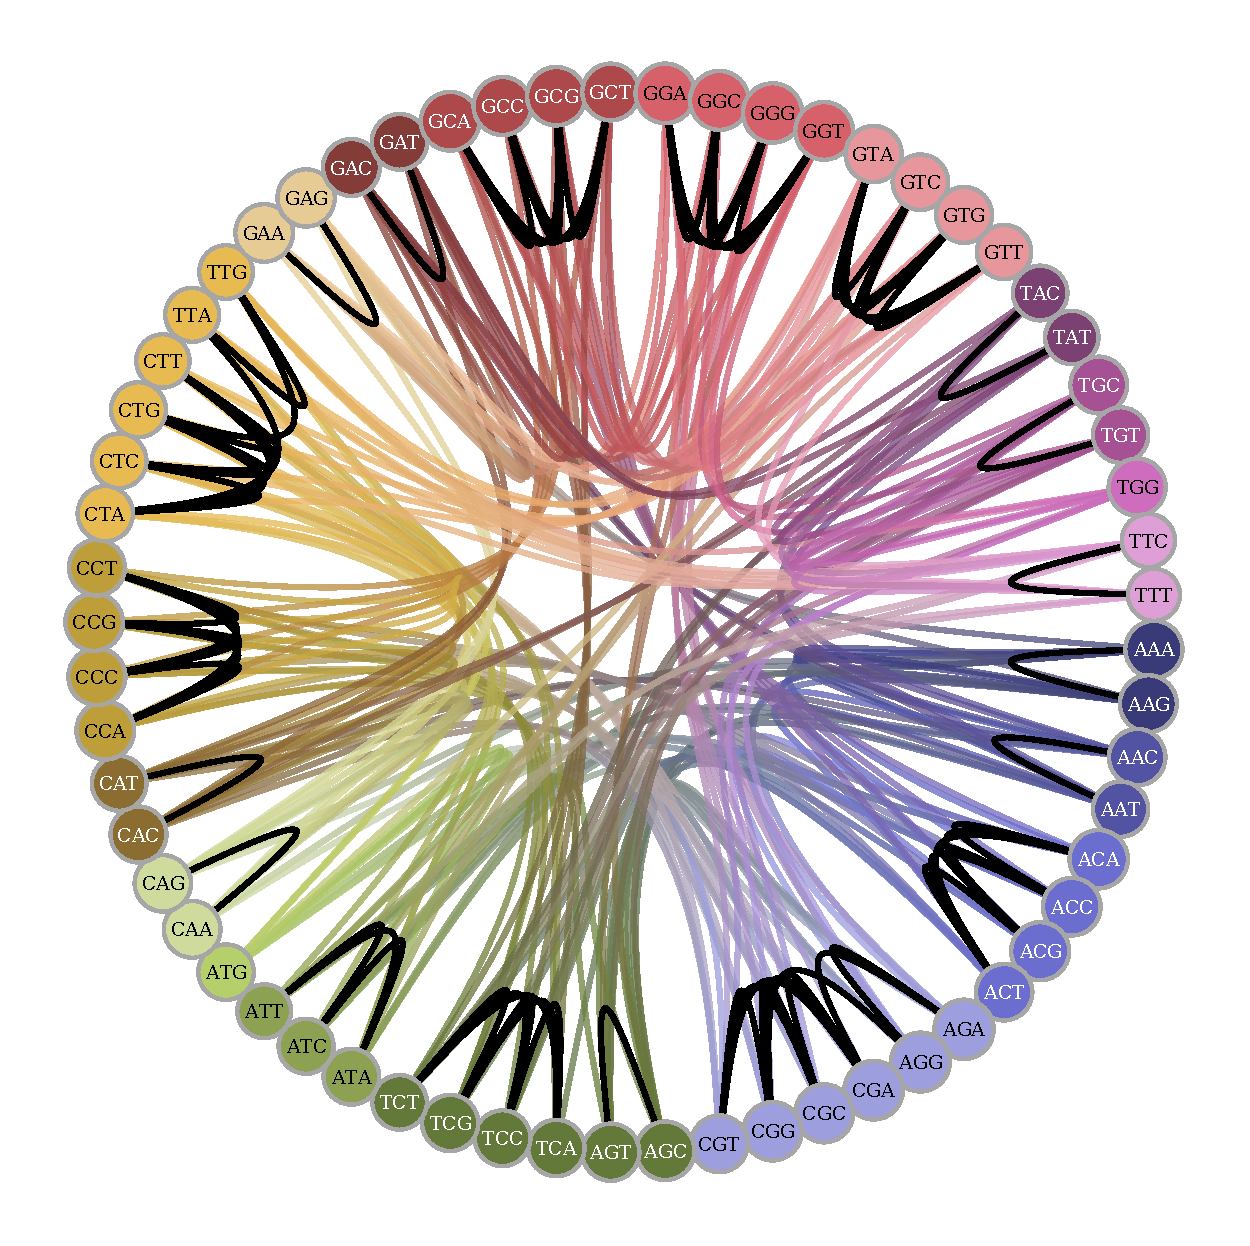
\includegraphics[width=\linewidth, page=1]{figures/gt-codon-tab20b.pdf}
		\end{minipage}%
		\hfill
		\begin{minipage}{0.49\linewidth}
			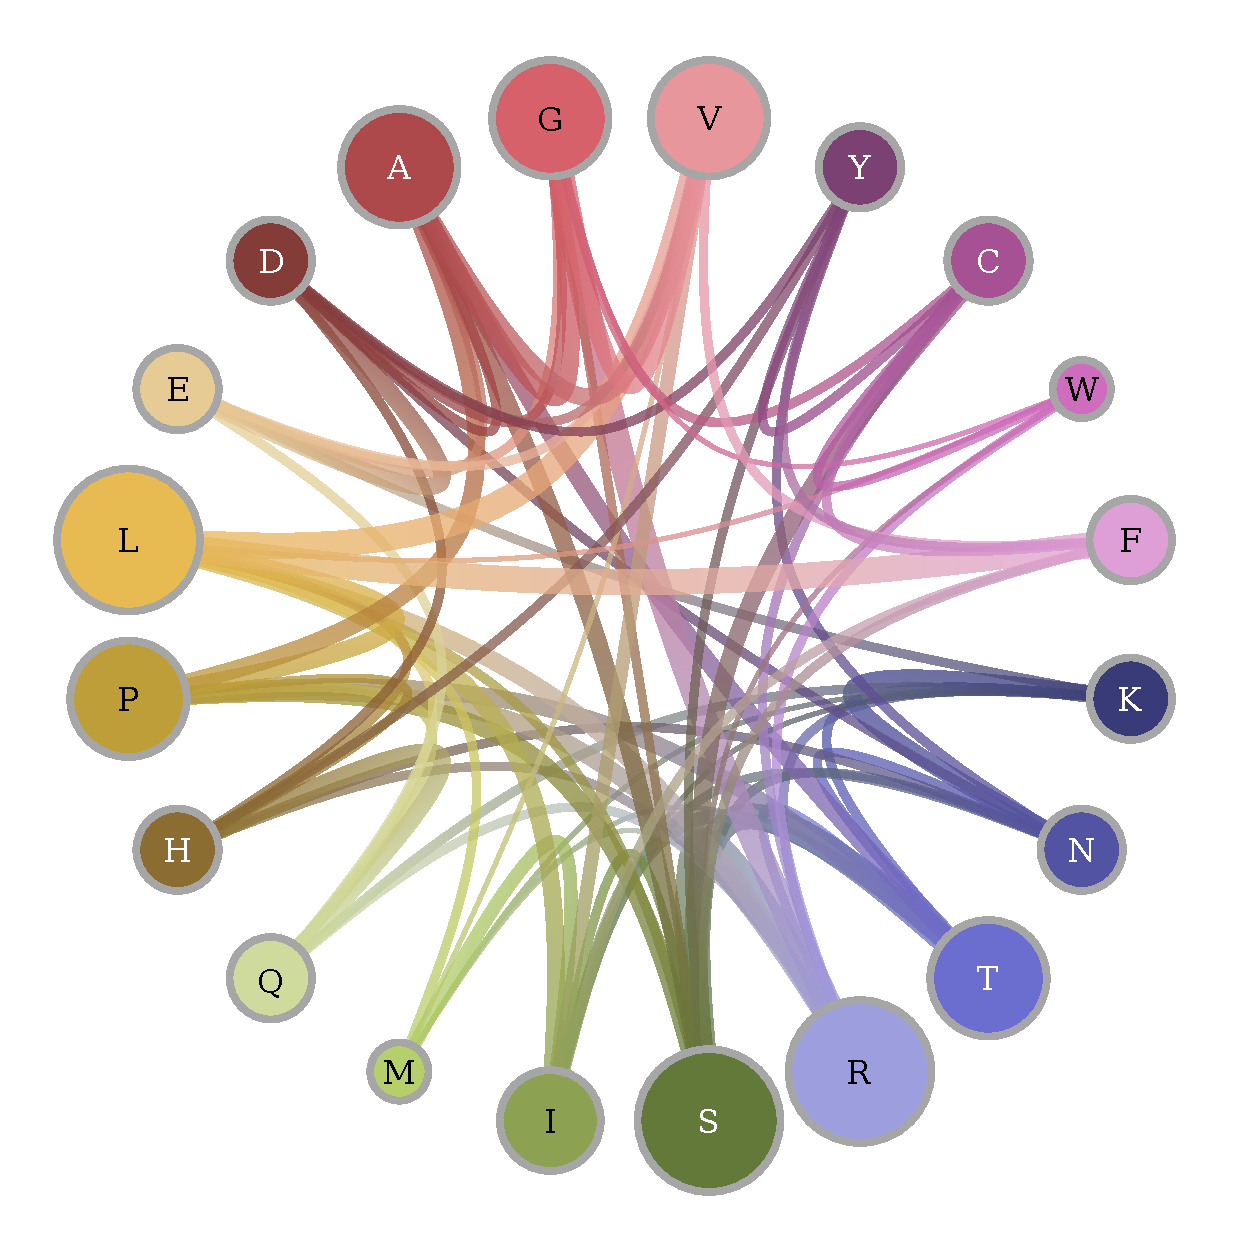
\includegraphics[width=\linewidth, page=1]{figures/gt-aa-tab20b.pdf}
		\end{minipage}

	\caption[Graphs of {codon} and amino-acid transitions]{
		\label{fig:graph-codons-aa}
		Graphs of possible one nucleotide {transition} between \gls{codon} (left panel) and between amino-acid (right panel).
		Nodes corresponds to \glspl{codon} (left panel) and amino-acid (right panel), where their color pictures the encoded amino-acid.
		Additionally, for amino-acids the size of nodes represent the number of underlying \glspl{codon}.
		An edge between two \glspl{codon} depicts a one nucleotide {transition}, such that a \gls{codon} can have at most $9$ possible {transitions}.
		Similarly, an edge between two amino-acids correspond to a one nucleotide non-synonymous {transition} between the underlying \glspl{codon}, and the weight of the edges represent the number of such possible {transitions}.
		Non-synonymous {transition} are represented in colored gradient, while synonymous {transitions} are depicted in black.
		The graph of the $61$ \glspl{codon} contains $263$ {transitions}, $67$ of them are synonymous while $196$ are non-synonymous.
		The radius of the graph is three, such that the most distant amino-acids are at most three {transition} away.
		Codons encoding for the same amino-acid are all fully connected by synonymous changes, expect for Serine where a {transition} for (TCT, TCG, TCC,	TCA) to (AGT, AGC) requires passing through another amino-acid, hence a least two non-synonymous {transitions}.
		From the perspective of amino-acids, the graph of the $20$ amino-acids contains $75$ non-synonymous {transitions}.
		The graph is not fully connected and do not form a clique. Moreover, the graph radius equal to three because a {transition} from Methionine to Tyrosine requires at least three non-synonymous {transitions}.
		Altogether, for all the possible $190$ pairs of amino-acids, $114$ pairs requires at least two non-synonymous {transitions}, and one pair (M-Y) requires at least three non-synonymous {transitions}.
	}
\end{figure}

\section{Protein thermodynamic}
\label{sec-intro:physic-protein}

\subsection{Stability constrains}

The ability of a protein to performs its function depends on the stability of its 3-dimensional folding structure, but also on its ability to bind ligands and interact or no with other protein, both in terms of kinetic and stability.
Altogether, thermodynamics and kinetic of protein are expected to be related to its function, hence to selective constrains~\citep{Bastolla2017}.
This section review the main relationship between protein biophysics and selection.

First, a large body of evidence indicates that the stability of globular proteins is a target of natural selection~\citep{Sikosek2014}.
The stability of a protein is determined by the Gibbs free energy of its folded states, in comparison to the free energy of the unfolded states.
Similarly to the mutation-selection Markov process defined in the previous chapter, it is possible to derive the equilibrium distribution of states, where fitness is analogous to the opposite of free energy (less energetic state are more stable) and population size to inverse temperature.
As a result, probabilities of observing a specific state, given by Boltzmann equation, is proportional to the exponential of free energy:
\begin{align}
	p(G_F)\propto \e^{- G_F / T}.
\end{align}
In this context, mutations of the proteins stabilizes the protein only if the decrease the free energy of the folded states, more than they decrease the free energy of unfolded states.
For example, a {transition} to an amino-acid that decrease by the same amount the free energy of both folded and unfolded states will have no impact on the stability of the protein.
Theoretically, the stability of a protein can be computed with biophysical of protein, by modeling the atomic structure and the potential energy of contact between residues, computed using Schrodinger's equation and atomic orbitals \textcolor{GREEN}{[References needed]}.
On the other extreme, some models more crudely approximates the structure and dynamic of protein by 2-dimensional lattice models with regular pavement \textcolor{GREEN}{[References needed]}. 
In between these two extremes, many models can approximate with various degrees of liberties and parametrization the relationship from sequence to stability.
Broadly, {transition} from hydrophobic to hydrophilic amino-acids at the surface of protein results in increase stability, and conversely for the protein core.

If the relationship from protein sequence to protein stability is within reach and can be obtained with various degrees of approximations, relationship from stability to fitness is more elusive and difficult to apprehend.
First, it is known the protein stability relates to fitness, as demonstrated by a study of nearly 1000 mutations in beta-lactamase TEM-1~\citep{Jacquier2013}, or illustrated by the use of functional assays to identify stabilizing mutations~\citep{Araya2012}.
However, it is not clear whether protein stability increases fitness by being more efficient, or whether it is the deleterious cytotoxic effect of unfolded proteins that result in purifying selection for destabilizing mutations.
Stability-constrained models that take into account negative design for destabilizing misfolded conformations.
At partial answer can be obtained by realizing that~\citep{Berezovsky2007, Noivirt-Brik2009, Minning2013} predict that both the \gls{substitution} rate and the entropy are maximal not at exposed sites with few contacts, as observed, but at sites where the number of contacts is intermediate, which can accomodate both hydrophobic and polar amino acids and are predicted to be extremely tolerant to mutations~\citep{Jimenez2018}.
On the other hand, when stability with respect to misfolding is not considered, stability-constrained models predict that the variability is maximal at exposed sites with few contacts~\citep{Scherrer2012,Echave2015}, but these kinds of models overestimate both the tolerance to mutations and the average hydrophobicity at almost all positions~\citep{Jimenez2018} and they score much worse than models that consider misfolding in \gls{likelihood} calculations~\citep{Arenas2015a, Arenas2017}, so that models that consider misfolding have to be preferred.
These results support the view that the structural effect of mutations cannot be neglected, in particular at sites with intermediate numbers of contacts that are extremely tolerant to mutations under the point of view of the stability.
Starting from an optimal sequence, mostly destabilizing mutations will occur, but they may reach fixation and accumulate until selection coefficients against new deleterious mutations is too strong, at which point the protein will reach a point of equilibrium called marginal stability~\citep{Taverna2002, Bloom2007}.

Importantly, theoretical models also based on protein stability have been invoked to explain this negative correlation between $\dnds$ and expression level~\citep{Wilke2006, Drummond2008}, such that selection against protein misfolding induces abundant proteins to evolve to greater stability, where the protein is more constrained and evolve slowly~\citep{Serohijos2012}.

Finally, the ability to bind other proteins may interfere with stability against misfolding, and large functional movements may imply a stability cost.
Empirically, residues at functional sites are rarely optimal for stability, so that their mutation is often less destabilizing, while mutations that create new functions tend to be more destabilizing than average~\citep{Chi2016}.

\subsection{Aggregation avoidance}

So far, proteins have been seen as independent machinery of the cells, however within the cramped intra-cellular space, proteins are not independent entities but are interactions with the proteome, where protein may either be in free form or engaged in non-specific interactions~\citep{Yang2012, Zhang2013}.
In non-specific interactions at the protein surface, stabilizing amino-acids are hydrophilic and destabilizing amino-acids are hydrophobic, sticking to hydrophobic residues in other proteins~\citep{Dixit2013,Manhart2015}.
The misinteraction avoidance hypothesis predicts that, compared with lowly expressed proteins, highly expressed proteins disfavour residues that promote misinteraction, exhibit a lower misinteraction probability per molecule and have higher conservation for misinteraction-avoiding residues.

\section{Rate of evolution}
\label{sec-intro:rate-evolution}

Models of \gls{codon} \glspl{substitution}, developped more formally in chapter \ref{sec:phylo_codon_models}, can be to applied to protein coding \acrshort{DNA} sequences alignment to estimates the ratio of non-synonymous over \gls{synonymous} rates ($\dnds$).
More precisely, these models can provides estimates of $\dnds$ for the whole gene, for a specific site or for a specific branch of the tree, and whether the sequence evolves under positive or negative selection.
All non-synonymous mutations are considered equivalent, and $\dnds$ encompass the average strength of selection exercised on them.
Most importantly, $\dnds>1$ is absorbing the signals of an excess in the rate of \glspl{non-synonymous}, indicating that the protein is under adaptive evolution.
Conversely, a default of \glspl{non-synonymous}, leading to $\dnds<1$, means the protein is under purifying selection.
However, in practice, protein are typically under a mix of adaptation and purifying selection, thus typically leading to an $\dnds<1$ even in the presence of positive selection.
Most importantly to the scope of this manuscript, they \gls{codon} models proved to be very valuable to quantify and asses the selective constrains imposed on protein coding sequences.

Importantly, different implementations of phylogenetic \gls{codon} models have been proposed, which parameterize the mutation matrix and the \gls{codon} frequencies in different way~\citep{Muse1994, Goldman1994}, ultimately leading to variable fits of the data and different estimation of $\dnds$ on the same dataset.
However, and fortunately, estimation of $\dnds$ has been proved to be largely insensitive to the underlying \gls{codon} models~\citep{Spielman2018}, such that empirical estimation of $\dnds$ using different methods leads to comparable results.

\subsection{Variation across genes}

The increased availability of genomic data together with advancement of computing resources and algorithm prompted an extensive search for the major determining factor of a gene $\dnds$.
Surprisingly, the functional importance of a protein, widely thought to approximate the level of functional constraint, has only a minor role, whereas protein expression level (mRNA concentraion) is found to be a major determinant~\citep{Zhang2015}.
Most importantly, this relationship is negative such that genes with high expression level are under stronger purifying selection, or lower $\dnds$ at the level of the gene~\citep{Duret2000, Drummond2005a, Zhang2015}.
In unicellular organisms, the mRNA concentration of a gene varies across cell cycle stages and environments, but most studies used data collected from the mid-log phase of growth under rich media, which presumably reflect average concentrations across cell cycle stages.
In multicellular organisms, mRNA concentration data used are typically from the whole organism or are averaged from several examined tissues.
Because of the strong correlation between mRNA and protein concentrations, the negative correlation between protein concentration and evolutionary rate is also strong.

However, even for those proteins of comparable expression levels, their $\dnds$ still span several orders of magnitude~\citep{Drummond2008}.
Abundance likewise cannot account for the quasi log-normal distribution of $\dnds$ among genes in a genome, a fact observed from bacteria, yeast, worm, fly, mouse, and humans.
These observations suggest that protein abundance, although a major determinant of $\dnds$, is not its only causal variable.

\subsection{Variation across sites}

Appart from variation across genes, the strength of selection is not typically homogeneous along the protein sequence, and it has been rapidly recognized that the parameter $\dnds$ should not be estimated globally over the entire sequence.
In so-called site-specific phylogenetic \gls{codon} models, $\dnds$ is allowed to vary across sites, either via a finite mixture~\citep{Yang2001}, an infinite mixture~\citep{Huelsenbeck2006}, or as random effects from a parametric distribution~\citep{Lartillot2013}.
Site-specific models had been developed to detect specific site of the sequence under positive recurrent selection~\citep{kosiol_patterns_2008}, with a $\dnds>1$, but also proved to be very valuable models to correlate selective pressure and bio-chemical properties os specific sites.

Similarly to search for the determining factors of $\dnds$ at the gene level, extensive search had been conducted at the site level, within a protein.
The major determinant of site-specific $\dnds$ proved to be relative solvent accessibility, where site with higher solvent accessibility display a lower $\dnds$~\citep{Ramsey2011}.
It was later shown that the number of native inter-residue contacts formed by a protein site, which is negatively correlated with the solvent accessibility, is a stronger predictor of site-specific $\dnds$~\citep{Yeh2013}.
Altogether, $\dnds$ changes dramatically between exposed and buried sites in such a way that buried sites tend to evolve more slowly than exposed sites~\citep{Echave2016}.
Moreover, this relationship obtained by means of phylogenetic \gls{codon} models can be matched with experiment correlating protein site properties with allelic diversity within population.
In this context, relative solvent accessibility was also found to be a major determinant of adaptive evolution, with most adaptive mutations occurring at the surface of proteins~\citep{Moutinho2019}.

The observations that surface residues of globular proteins undergo \gls{substitution} more rapidly than those in the core is generally attributed to the fact that natural selection imposes stronger constraints on buried sites.
It is well known that amino acid residues located inside a protein structure (that is, core residues) have more central roles than surface residues in protein folding stability.

Finally, it is important to keep in mind that selection differs in a way that depends on the specific source and target amino-acid involved in the {transition}.
As a consequence, a single parameter of selection (here $\dnds$) can not disentangle the specific importance of amino-acid chemical properties (polarity, volume, charge, and so on) since all non-synonymous {transitions} are considered equivalent in classical phylogenetic \gls{codon} models~\citep{Dutheil2008}.

\subsection{Variation across branches}

Beside variation across genes and site, the strength of selection is not typically homogeneous along the phylogenetic tree, and it has also been recognized that the parameter $\dnds$ should be varying along the tree~\citep{Yang1998}.
The motivation was to allow for $\dnds$ to be estimated only on a subset of the phylogeny, based on biological assumption.
For example, such models can detect an adaptive process ongoing during the divergence of one lineage, which can allow for the detection of the proteins responsible for speciation~\citep{Yang2001, Zhang2004}.
Moreover, without \gls{prior} knowledge on biological divergence, branches can get clustered together based on their \gls{substitution} rates~\citep{Dutheil2012a}.
However, \gls{substitution} rate is a continuous traits, and should evolve smoothly along the phylogeny, such that abrupt shifts are penalized~\citep{Huelsenbeck2003,Seo2004}.
I this modeling approach, \gls{substitution} rate of given branch is log-normally distributed around the value of its parent branch, where the standard deviation is proportional to the branch size (in unit of time)~\citep{Lartillot2011, Brevet2019}.
In other words, \gls{substitution} rate is seen as a log-Brownian motion along the phylogeny, where the process splits at every node of the tree. 

Similarly to search for the determining factors of $\dnds$ at the gene and site level, environmental variables or life-history traits that can vary between species have been investigated as factor determining $\dnds$ along the phylogeny~\citep{Felsenstein1985,Romiguier2014}.
Integrative inference methods combining molecular sequences and lineage specific quantitative traits have also found that $\dnds$ correlates positively with traits such as longevity and body mass~\citep{Lartillot2011, Figuet2017}.
Since lineage with a large body size and extended longevity typically correspond to low $\Ne$~\citep{Romiguier2014}, these empirical correlations suggest a negative correlation between $\dnds$ and $\Ne$, thus confirming the theoretical prediction of the \gls{nearly-neutral} theory of evolution.
However, the universality and robustness of the correlation between $\dnds$ and life-history traits is still debated~\citep{Nabholz2013, Lanfear2014, Figuet2016}.

Naturally, both these space (site-specific) and time (branch-specific) refinements mentioned above where combined in so called branch-site models~\citep{Yang2002, Zhang2004, Pond2011}.
The fine-grained tunning of site-branch models increased statistical power by seeking short and strong episodes of adaptive selection on a background of purifying selection.
However, in the case of Red-Queen processes ongoing on the protein, the episodes detected by branch-site models would merely be a small fraction of the underlying adaptation.
Indeed the overall tree is under adaptive process and one cannot contrast a branch to the rest of the tree.

%The selection coefficient are drawn from a distribution, known as distribution of fitness effects~\citep{Welch2008}
%In Wilson, the fitness effect of a mutation is drawn from a fitness distribution that is solely function of $\Ne$, meaning ${P_{\mathrm{fix}}}$ is independent from the current sequence state.
%On the other hand, in the mutation-selection model proposed, the distribution of fitness effects is a function of the current state.
%
%Because its a distribution of fitness effects and not a fitness landscape, features of evolutionary trajectory such as transient positive selection is not represented.
%They are a generic representation of fitness, easily parameterized and inherently taking into account phenomenon such as epistasis.


\chapter{Phylogenetic Bayesian models}
{
	\hypersetup{linkcolor=GREYDARK}
	\minitoc
}
\label{sec:phylo_bayes}
The previous chapter treated how \gls{substitution} rates are defined and parameterized, but not how these parameters are inferred and estimated.
Given a set of observed protein-coding \acrshort{DNA} sequences in different species or lineages, the goal is to estimates the underlying parameters of evolution.
However, models of \glspl{substitution} presented so far are not sufficient to fulfills this endeavor, but instead can be used to generate a random trajectory of protein-coding \acrshort{DNA} sequence evolution.
Indeed, given parameters of evolution, simulations using the \gls{substitution} rates between \glspl{codon}, when run along a phylogenetic tree, can give us a likely representative protein coding \acrshort{DNA} sequence for each extant species (at the tip of the tree), producing an alignment. 
Moreover by running several random simulations, one can expect to obtain representative and likely set of alignments.
Unfortunately, even with huge amount of simulations, it is very unlikely to generate precisely our observed alignment, and even more difficult to precisely pin down the probability of our observed alignment to have been generate by a given set of parameters.
Deriving this probability of observing a specific alignment given the parameters is thus the first theoretical question to answer, which is the focus of the first section.
With this analytical probability obtained, it is then possible the derive for different sets of parameters their respective probability of generating the observed alignment.
The next endeavor is thus to reverse the question, and instead of having the probability of the alignement given the parameters, the goal is to derive the probability of the parameters given the alignment.
This subsequent endeavor is thus the focus of the second section, recalling theoretical and computational implementation of Bayesian inference, in the context of phylogenetic \gls{codon} models.

\section{Likelihood of the data}

For a dataset of protein-coding \acrshort{DNA} sequences, the goal is to determine the probability of the observed sequence data at the tips of the tree conditional upon the evolutionary model, the tree, and values of parameters in the model.
The challenge is that only the data for the extant species are observed whereas the sequence at the root of the tree and the subsequent evolutionary events are not directly observed.
In other words, all possible trajectories leading to the observed alignment must be integrated, weighted by their respective probabilities.

Throughout this development, the tree topology ($\tau$) is considered know and fixed.
This restriction emanates that the scope of this is work is not to infer the topology, but the parameters of evolution.
Moreover, the development does not delves into the details of how alignment are obtained, and thus assume that they are correct.
However it has been shown that outputs of different sequence alignment methods tend to produce different results that are not consistent.
The main determining factor of alignment accuracy is evolutionary divergence, such that if alignment are restricted to orthologs from closely related taxa, or to slow-evolving genes, alignment errors become scarce and may not cause significant encumbrance.
Finally, and not the least, models of sequence change will assume that changes at one sequence position have no impact on whether other positions will change.
This assumption of independence between sites allows the probability of an observed set of aligned sequences at the tips of an evolutionary tree to be expressed as the product over alignment columns of the observed nucleotides or amino acids in those columns. 
This independence assumption is simplistic, throwing away biological information, and can be shown statistically to be problematic, but permits computationally convenient likelihood-based inference.

The section is divided into first integrating over all trajectory over a single branch of tree, and subsequently over the total tree. And finally efficiently computing the probability of observed data given the parameters.

\subsection{Probability of {transitions} for a branch at a given site}
Point \gls{substitution} process define the instantaneous rates of change between the different \glspl{codon} through the \gls{substitution} matrix $\Submatrix$.
However, given a starting state of the process (ancestral) and a given amount of time for which the \gls{substitution} process runs, it is possible to derive the probability of the descendant sequence having each of the $61$ \gls{codon} states.
In practice, time is measured in unit of branch length, expressing the expected number of changes to have occurred since the ancestor if {transition} are \gls{neutral}.
For example of branch length of $2$ imply that $2$ changes are expected to be seen on average along the branch under the condition that \glspl{substitution} are \gls{neutral}.
Consequently, the \gls{substitution} rate matrix must be normalized to be measured in unit of branch length, where in practice instead of normalizing the \gls{codon} subtitution matrix, the nucleotide mutation matrix is normalized since mutation are considered \gls{neutral}.
The mathematical details of this transformation from rate-matrix to probability matrix are described from first order derivation of the Markov process.
At a give site ($\site$) of the sequence, and along a given branch ($\branch$) with branch length $\branchlength\branchexp$, the \gls{codon} probability matrix $\Probmatrix\siteexp(\branchlength\branchexp)$ is related to the {transition} matrix ($\Submatrix\siteexp$ at site $\site$) trough the first-order differential equation:
\begin{align}
	\dfrac{\der \Probmatrix\siteexp(\branchlength\branchexp)}{\der \branchlength\branchexp}	& = \Probmatrix\siteexp(\branchlength\branchexp) \Submatrix\siteexp, \\
	\iff \Probmatrix\siteexp(\branchlength\branchexp) & = \e^{\branchlength\branchexp \Submatrix\siteexp}.
\end{align}
The integration of the \gls{substitution} rate matrix over the branch length entails to take into all possible trajectories histories of evolutionary events, leading to a compact probability matrix computed as an exponential of the rate matrix.
In practive, exponential of the rate matrix is usually performed using eigenvalues and eigenvectors decomposition.

\subsection{Total probability of transition}
The challenge to generalize from branch to tree is that only the data at the tips of the tree are observed whereas the states of the internal nodes are not directly observed.
As a result, \gls{likelihood} of the observed data can be readily calculated if the ancestral state of all internal node is know, from the probabilities of {transitions} along each branch of the tree.
As an example for better readability, a simple illustrative tree given in figure \ref{fig:tree} will be used \gls{prior} to giving to general formulas.
\begin{figure}[H]
	\centering
	\begin{tikzpicture}[->,>=stealth',shorten >=1pt,auto,node distance=0.6cm and 1.2cm,semithick]
	\tikzstyle{every state}=[]

	\node[state] (1) [dashed, BLUE] {$\state_1$};
	\node[state] (0) [YELLOW, below right=of 1] {$\state_0$};
	\node[state] (2) [BLUE,below left=of 0] {$\state_2$};
	\node[state] (5) [YELLOW,right=of 0] {$\state_5$};
	\node[state] (3) [BLUE,above right=of 5] {$\state_3$};
	\node[state] (4) [BLUE,below right=of 5] {$\state_4$};

	\path[-]
	(1) edge [black] node [above right] {$\branchlength^{(1)}$} (0)
	(2) edge [black] node [below right] {$\branchlength^{(2)}$} (0)
	(5) edge [black] node [above] {$\branchlength^{(5)}$} (0)
	(5) edge [black] node [above left] {$\branchlength^{(3)}$} (3)
	(5) edge [black] node [below left] {$\branchlength^{(4)}$} (4);
	\end{tikzpicture}
	\caption[Illustrative phylogenetic tree]{
	Illustrative phylogenetic tree. Internal nodes ($\state_0$ and $\state_5$) are represented in yellow, while extant nodes ($\state_1$ to $\state_4$) for which the state is know from the observed data is represented in blue. The node $0$ is considered the root of the tree, although defining is not strictly required since the process is reversible.}
	\label{fig:tree}%
\end{figure}

In the example of the illustrated tree, from the observed data for the extant nodes $\Data\siteexp = \{ \state_1,\state_2, \state_3, \state_4 \}$, at site $\site$, the \gls{likelihood} given that the states of the internal nodes are known is computed as:
\begin{align}
	p\left(\Data\siteexp| \state_0, \state_5, \Submatrix\siteexp, \branchlength\branchexp, \forall \branch \right) & = \Probmatrix\siteexp_{\state_0, \state_1}(\branchlength^{(1)})
	\Probmatrix\siteexp_{\state_0, \state_2}(\branchlength^{(2)}) \\
	& \quad \quad \quad
	\times \Probmatrix\siteexp_{\state_5, \state_3}(\branchlength^{(3)})
	\Probmatrix\siteexp_{\state_5, \state_4}(\branchlength^{(4)})
	\Probmatrix\siteexp_{\state_0, \state_5}(\branchlength^{(5)}) \notag
\end{align}
In the general topology, $\Data\siteexp = \{ \state_P \hdots \state_{2P-1} \}$, where $\state_{\nodeUp}$ and $\state_{\nodeDown}$ are used to denoted the respectively the parent and descendant nodes of a branch, the \gls{likelihood} of the observed data is given as:
\begin{align}
p\left(\Data\siteexp| \state_{I}, \Submatrix\siteexp, \branchlength\branchexp, \forall (I, \branch) \right) & = \prod_{b} \Probmatrix\siteexp_{\state_{\nodeDown}, \state_{\nodeUp}}(\branchlength^{(\branch)}),
\end{align}
where $I$ runs over all the internal nodes.

Because the states of the internal nodes are not actually unknown, the \gls{likelihood} must be summed over the all the possible states, weighted by their equilibrium stationary frequencies ($\pi\siteexp$).

In the case of the illustrative example, the total probability is given as
\begin{align}
	p\left(\Data\siteexp| \Submatrix\siteexp, \branchlength\branchexp , \forall \branch \right) & = \sum_{\state_0=1}^{61} \subequi_{\state_0} \sum_{\state_5=1}^{61} \subequi_{\state_5} p\left(\Data\siteexp| \state_0, \state_5, \Submatrix\siteexp, \branchlength\branchexp \right) \\
	& = \sum_{\state_0=1}^{61} \subequi_{\state_0} \sum_{\state_5}^{61} \subequi_{\state_5} \Probmatrix\siteexp_{\state_0, \state_1}(\branchlength^{(1)})
	\Probmatrix\siteexp_{\state_0, \state_2}(\branchlength^{(2)}) \\
	& \qquad \qquad \qquad
	\times \Probmatrix\siteexp_{\state_5, \state_3}(\branchlength^{(3)})
	\Probmatrix\siteexp_{\state_5, \state_4}(\branchlength^{(4)})
	\Probmatrix\siteexp_{\state_0, \state_5}(\branchlength^{(5)})\notag
\end{align}

And because the process is reversible, the equilibrium frequencies of \glspl{codon} satisfies the equations:
\begin{align}
\bm{0} & = \bm{\pi}\branchsiteexp \Submatrix\branchsiteexp \\
\iff \bm{\pi}\branchsiteexp & = \bm{\pi}\branchsiteexp \Probmatrix\branchsiteexp \\
\iff \dfrac{\subequi_{\ci}\siteexp}{\subequi_{\cj}\siteexp} & = \dfrac{\submatrix_{\cj, \ci}\siteexp}{\submatrix_{\ci, \cj}\siteexp}
\end{align}

In the general topology, the \gls{likelihood} of the observed data is thus given as:
\begin{align}
p\left(\Data\siteexp| \Submatrix\siteexp, \branchlength\branchexp, \forall \branch \right) & = p\left(\Data\siteexp| \state_{I}, \Submatrix\siteexp, \branchlength\branchexp, \forall (I, \branch) \right), \\
& = \sum_{\state_{0}=1}^{61} \subequi_{\state_{0}} \hdots \sum_{\state_{k}=1}^{61} \subequi_{\state_{k}} \prod_{b} \Probmatrix\siteexp_{\state_{\branch^{+}}, \state_{\branch^{-}}}(\branchlength^{(\branch)}), \label{eq:likelihood-site}
\end{align}

And finally, the assumption of independence between sites allows the probability of an observed set of aligned sequences at the tips of an evolutionary tree to be expressed as the product over alignment columns of the observed nucleotides or amino acids in those columns:
\begin{align}
p\left(\Data| \Submatrix\siteexp, \branchlength\branchexp, \forall (\site, \branch) \right) & = \prod_{\site} p\left(\Data\siteexp| \Submatrix\siteexp, \branchlength\branchexp, \forall \branch \right) \label{eq:likelihood}
\end{align} 
\subsection{Pruning algorithm}
The \gls{likelihood} of observed data at a specific column of a multiple sequence alignment, given by equation \ref{eq:likelihood} requires extensive computation, but can however can be determined with the pruning algorithm of \citet{Felsenstein1985}. 
The \gls{likelihood} of the data $\Data$ can be computed using the pruning algorithm:
\begin{align}
p\left(\Data\siteexp| \Submatrix\siteexp, \branchlength\branchexp, \forall \branch \right) & = \sum_{\ci=1}^{61} \subequi\siteexp_{\ci} \pruning\siteexp_{0} \left( \ci \right)
\end{align}
where $\pruning_{\node} \left( \ci \right)$ is computed recursively from the $2$ descendant children $\node_{1}$ and $\node_{2}$ of an internal node $\node$:
\begin{align}
\pruning\siteexp_{\node} \left( \ci \right) = 
\left[ \sum_{\cj=1}^{61}\Probmatrix\siteexp_{\itoj}(\branchlength^{(\node \to \node_{1})}) \pruning\siteexp_{\node_{1}} \left( \cj \right) \right] 
\cdot 
\left[ \sum_{\cj=1}^{61}\Probmatrix\siteexp_{\itoj}(\branchlength^{(\node \to \node_{2})}) \pruning\siteexp_{\node_{2}} \left( \cj \right) \right] 
\end{align}
And if the node $\node$ is a node with no descendant, meaning an extant taxa:
\begin{align}
\pruning\siteexp_{\node} \left( \ci \right) =
\begin{dcases}
1, & \text{if } \state_{\node} = \ci \\
0, & \text{otherwise.}
\end{dcases}
\end{align}

\section{Bayesian estimation}
The Bayesian Paradigm can be seen as a way to model uncertainty in a probabilistic way.
In other words, parameter of the models denoted $\theta$ are considered as random variables whose distribution describes that uncertainty.
This unconditional distribution of parameters, $p(\theta)$, is called the \gls{prior}.
The probability of those parameters are going to be modified after acquisition of information supplied by observed data.
More precisely, Bayes theorem is essential in updating of the distribution :
\begin{equation}
	p(\theta|\data)=\frac{p(\data|\theta)p(\theta)}{p(\data)}
\end{equation}
The probability of the parameters matrix $\theta$ given the data is called the \gls{posterior} probability, it is \gls{posterior} to the data, and $p(\data|\Probmatrix)$ is the 

Because the actual probability of the data is not going to change, in inference Bayes theorem is often presented as:
\begin{equation}
p(\data|\data) \propto p(\data|\data)p(\data)
\end{equation}
Simply stating that the \gls{posterior} is proportional to the \gls{likelihood} time the \gls{prior}.

From the \gls{likelihood} of the data derived in the previous section, the difficulties now is shifted to the definition of the \gls{prior} distribution, where these difficulties come in two flavors.
Firstly, the parameters of evolution for which \gls{prior} distribution can be apprehended might be the parameters of interest such as the selection coefficient, or on the mutation rate, but not the \gls{prior} distribution of the \gls{substitution} rate matrix as a whole.
This difficulties is eased by Bayesian network, which are a probabilistic graphical representation of a set of variables and their conditional dependencies via a directed acyclic graph (DAG).
In the example of the \gls{prior} distribution for the rate \gls{substitution} matrix, it is determined as the joint distribution of the \gls{prior} over the selection coefficient and the mutation rate matrix, which itself is given by the joint distribution over the equilibrium frequencies of nucleotides and exchangeabilities rates for the general-time-reversible (GTR) mutation matrix (see figure \ref{fig:DAG}).
Seeing the DAG the other way around (following the arrows), simple \gls{prior} distribution are combined together to form more complex joint \gls{prior} distribution which ultimately define the \gls{prior} distribution of the model ($\theta$).

\begin{figure}[H]
	\centering
	\begin{tikzpicture}[->,>=stealth',shorten >=1pt,auto,node distance=0.6cm and 1.2cm,semithick]
	\tikzstyle{every state}=[]
	
	\node[state] (P) {$\Probmatrix\siteexp(\branchlength\branchexp)$};
	\node[state] (Q) [below right=of P] {$\Submatrix\siteexp$};
	\node[state] (BL) [BLUE, above right=of P] {$\branchlength\branchexp$};
	\node[state] (Exp) [RED, right=of BL] {$1$};
	\node[state] (F) [below right=of Q] {$\bm{F}\siteexp$};
	\node[state] (sb) [BLUE, right=of F] {$W$};
	\node[state] (sbH) [RED, right=of sb] {$\stickbreakinghyper$};
	\node[state] (R) [above right=of Q] {$\Mutmatrix$};
	\node[state] (Ex) [BLUE, above right=of R] {$\Exchan$};
	\node[state] (ExH) [RED, right=of Ex] {$\dfrac{1}{6}, 6$};
	\node[state] (Equi) [BLUE, below right=of R] {$\Mutequi$};
	\node[state] (EquiH) [RED, right=of Equi] {$\dfrac{1}{4}, 4$};
	
	\path 
	(Q) edge [black] node [above right] {} (P)
	(BL) edge [black] node [] {} (P)
	(Exp) edge [dashed, BLUE] node [above] {\textit{Exp}} (BL)
	(R) edge [black] node {} (Q)
	(Ex) edge [black] node [] {} (R)
	(Equi) edge [black] node [below] {} (R)
	(ExH) edge [dashed, BLUE] node [above] {\textit{Dir}} (Ex)
	(EquiH) edge [dashed, BLUE] node [above] {\textit{Dir}} (Equi)
	(F) edge [black] node {} (Q)
	(sb) edge [black] node [above] {} (F)
	(sbH) edge [dashed, BLUE] node [above] {\textit{DP}} (sb);
	\end{tikzpicture}
	\caption[Directed acyclic graph of Bayesian network]{
	Directed acyclic graph of dependencies between variables.
	Nodes of the directed acyclic graph are the variables, and edges are the functions. Hyper-parameters are depicted in {\color{RED}{red}} circle, random variables in {\color{BLUE}{blue}} circles, and transformed variables in black.
	{\color{BLUE}{blue}} solid line denotes a drawing from a random distribution, and black solid lines denote a function.
	\textit{Exp} denotes an exponential distribution, \textit{Dir} denotes a Dirichlet distribution, and finally \textit{DP} denotes a \gls{Dirichlet-process}.}
	\label{fig:DAG}
\end{figure}

Secondly, once realizing that the \gls{prior} distribution can be boiled to a set of simpler \gls{prior} distributions, the difficulty arise from the high dimensionality of the parameter space, known as the curse of dimensionality.
More precisely, the number of states increases exponentially with the number of dimension of the space, such that the space is too large to be explored and computation of both the \gls{prior} and the \gls{likelihood} for each set of parameters is unrealistic.
Reduction in the exploration of the state space is obtained by employing Monte-Carlo Markov-Chain, which effectively approximate the target \gls{posterior} distribution.

\subsection{Monte-Carlo Markov-Chain}

The first \acrshort{MC} algorithm is associated with the army laboratory in Los Alamos under the direction of Metropolis in early 1952.
Both a physicist and a mathematician, Nicolas Metropolis was one of the first scientists to work on the Manhattan Project that led to the production of the atomic bomb.
Almost as early, he became obsessed with the hydrogen bomb, which he eventually succeed in building.

Published in June 1953 in the \textit{Journal of Chemical Physics}, the primary focus of \acrshort{MC} algorithm is computing the energy of random configurations for a system of many particles.
This energy is not not available analytically and requires integration across for all realizations of the random configurations of the particle system.
Because the number of dimensions is high (twice the number of particles), numerical integration is impossible using a deterministic algorithm.
Moreover, because the probability of a given configuration can be very small, even Monte Carlo integration, by sampling randomly across the target distribution of configurations fails to correctly approximate this integral.

This problem can however be transposed in the \gls{mc} realm, where each state of the process is a particular configuration of particles.
The {transition} probabilities between states must generate a stationary distribution equal to the target distribution of particle configurations.
Given this requirement, and given we can also sample from the {transition} probabilities, the Monte Carlo \gls{mc} starts from a given state and can be updated by random sampling from the {transition} probabilities.
The chain is composed of a period of burn-in, where the current state is of low probability relative to more likely states.
Once reaching the dynamic equilibrium, the energy of each configuration can be computed and the average of this energy is an approximate solution for the integral of energy over the distribution of configurations.


\subsection{Metropolis-Hastings sampling}

The Metropolis algorithm is an acceptance/rejection rule for the probabilities of {transition} allowing to match the stationary distribution to the specified target distribution, present in the original paper.
From a state $X_t$, the algorithm proceeds as follows at each step of the \gls{mc}:
\begin{itemize}
	\item Generate a random candidate state $X'$ according to $g(X'\mid X_t)$.
	\item Calculate the acceptance ratio $\displaystyle r=\min \left(1,{\frac {P(X')}{P(X_{t})}}{\frac {g(X_{t}\mid X')}{g(X'\mid X_{t})}}\right)$.
	\item Generate a uniform random number $u\in [0,1]$.
	If $u\leq A(X',X_{t})$, then accept the new state and set $X_{t+1}=X'$.
	Else reject the new state and set $X_{t+1}=X$
\end{itemize}

The algorithm requires the ability to calculate the acceptance ratio $r$ for all possible jump, and to draw a jump from any state. 
In addition, last step above requires the generation of a uniform random number.
The Metropolis procedure has been developped in the context of a symmetric distribution $g(X'\mid X) = g(X \mid X')$, and was later generalized to incorporate any distribution, such that the factor $g(X'\mid X) / g(X \mid X')$ took the name Hasting ratio.

\subsection{Gibbs sampling}

Gibbs sampling is applicable when a joint distribution of variables is not known explicitly or is difficult to sample from directly, but the conditional distribution of each variable are easier to sample from.
The original implementation of the Gibbs sampler was applied to a discrete image processing problem, a problem somewhat removed from statistical inference in the classical sense.
This paper is also responsible for the name {\it Gibbs sampling}, because it implemented this method for the Bayesian study of {\it Gibbs random fields} which, in turn, derive their name from the physicist Josiah Willard Gibbs (1839-1903).

The individual variables are sampled one at a time, with each variable conditioned on the most recent values of all the others.
It can be shown that the sequence of samples constitutes a \gls{mc}, and the stationary distribution of that \gls{mc} is just the joint distribution.
Gibbs sampling is particularly well-adapted to sampling the \gls{posterior} distribution of a Bayesian network, since they are composed of a set of individual random variables in which each variable is conditioned on only a small number of other variables.

Gibbs sampling can be considered a general framework for sampling from a large set of variables by sampling each variable (or in some cases, each group of variables) in turn.
Various algorithms can be used to sample these individual variables, depending on the exact form of the multivariate distribution, it can incorporate the Metropolis–Hastings algorithm, or more sophisticated methods such as slice sampling, adaptive rejection sampling and adaptive rejection Metropolis.

\subsection{Sufficient statistics \& data augmentation}

The basic idea is to augment the observed sequence data with a possible \gls{substitution} history and to then use \gls{mc} Monte Carlo techniques to perform a random walk over histories that are consistent with the observed data.

A realization of the random process results in a detailed \gls{substitution} history over the tree.
Most phylogenetic Monte-Carlo-Markov-Chain (\acrshort{MC}) samplers target the distribution over the model parameters, which means that they have to repeatedly invoke the pruning algorithm to recalculate
the pruning-based \gls{likelihood} which is most often the limiting step of the \acrshort{MC}.

An alternative, which is used here, is to do the \acrshort{MC} conditionally on the detailed \gls{substitution} history $\subhistory$, thus doing the \acrshort{MC} over the augmented configuration~($\subhistory$, $\data$), under the target distribution obtained by combining the mapping-based \gls{likelihood} with the \gls{prior} over model parameters

The key idea that makes this strategy efficient is that the mapping-based \gls{likelihood} depends on
compact summary statistics of $\subhistory$ (which in turn depend on the specific parameter component
being resampled), leading to very fast evaluation of the \gls{likelihood}.
On the other hand, this requires to implement more complex \acrshort{MC} procedures, that have to alternate between:

1) sampling $\subhistory$ conditionally on the data and the current parameter configuration.

2) re-sampling the parameters conditionally on $\subhistory$.

To implement the mapping-based \acrshort{MC} sampling strategy, we first sample the detailed \gls{substitution} history $\subhistory$ for all sites along the tree.
Several methods exist for doing this \citep{Nielsen2002,Rodrigue2008}.
Then, we write down the probability of $\subhistory$ given the parameters, and finally, we collect all factors that depend on some parameter of interest and make some simplifications.
This ultimately leads to relatively compact sufficient statistics (Supplementary Materials for the different sufficient statistics used by our model) that are fast to evaluate \citep{Irvahn2014,Davydov2016}.



\chapter{Goals of the thesis}
{\hypersetup{linkcolor=GREYDARK}\minitoc}
\label{chap:goals}

Nearly-neutral theory of evolution, introduced historically in chapter \ref{chap:intro-historical}, had broad implications in evolutionary biology and molecular evolution.
In this context, evolution of molecular sequences is seen as a stochastic process, where one component of this process is creating diversity through mutation, another antagonistic component is filtering out this diversity through selection, and finally the balance between these components is arbitrated by drift, formally presented in chapter \ref{chap:intro-formalism}.
Applied to protein coding DNA sequences, this stochastic process results in a pattern of substitution along of species tree, where phylogenetic codon models presented in chapter \ref{chap:intro-codon-models} captures intrinsic parameters of evolution.
How such parameters are inferred from an contemporaneous protein coding DNA sequences is described and developed in \ref{chap:intro-inference}.
Finally, selection of protein coding is related to biophysical constrains and thermodynamic properties of protein, such as to model selection acting on protein coding DNA sequences from physical first principles illustrated in chapter \ref{chap:intro-physic-proteins}.

In this context, this thesis is a modest attempt to disentangle interaction between mutation, selection and drift, from patterns found in contemporaneous protein coding DNA sequences.
I confront theoretical development to empirical data, whether through analytical results, simulation and inference.
The results are divided in three chapters, each written in the form of independent manuscript that shall be submitted to peer-reviewed journals.
Firstly, because the composition of protein coding DNA sequences does not reflect the underlying mutational process, but its filtering by selection at the level of amino-acids, a careful phenomenological modeling is necessary to uncover mutational process and nucleotide fixation bias, a study presented in section ~\ref{sec-goals:NucleotideBias} and developed in chapter~\ref{chap:NucleotideBias}.
Secondly, the balance between mutation and selection is arbitrated by drift, which is mediated by effective population size and its changes along a phylogeny can be estimated by mechanistic codon models, a study presented in section ~\ref{sec-goals:MutSelDrift} and developed in chapter~\ref{chap:MutSelDrift}.
Finally, selection for protein stability imply an analytical relationship between the rate of evolution and effective population size and protein expression level, a study presented in section ~\ref{sec-goals:GenoPhenoFit} and developed in chapter~\ref{chap:GenoPhenoFit}.

\section{Robustness of codon models to mutational bias}
\label{sec-goals:NucleotideBias}

Nucleotide composition in protein-coding sequences is the result of the equilibrium between mutation and selection.
However, by capturing selection through a single parameter $\omega$, classical codon model (see chapter \ref{chap:intro-codon-models}) can risk mistaking the mutational process, which is corroborated by some observations. 
Indeed, codon model parameterized by a single mutation rate matrix predicts that the nucleotide composition is the same for all $3$ positions of the codons.
However it as empirically been observed that the nucleotide composition of protein coding sequences are not identical, with the third positions showing more extreme composition than first and second position.
Alternatively, to accommodate such variation across positions, some models allow for different nucleotide rate matrices at the three positions, an approach which is problematic since the mutation process should in principle be blind to the coding structure, and should be homogeneous across coding positions.
Although this misconception has probably minor impact on detection of positive selection, it is clear symptom of a more fundamental issue with teasing apart mutation rates and fixation biases in codon models.
Practically, this could have important consequences in the current interest for detecting traces of biased gene conversion toward GC (gBGC) in protein coding sequences, a factor which requires mutation and fixation biases to be disentangled.
In this context, chapter \ref{chap:GenoPhenoFit} presents an alternative modeling approach, where $\omega$ is seen as a tensor, an array of $\omega$ values unfolding along multiple directions, an  is test to empirical and simulated protein coding DNA alignment.

\section{Inferring long-term population size}
\label{sec-goals:MutSelDrift}

Presented in section \ref{sec:intro-classical-codon-models}, mechanistic phylogenetic codon model are grounded on population-genetics first principles and articulates the interplay between mutation, selection and drift.
These recently models return site-specific estimate of amino-acid fitness landscape, but they rely on the assumption of constant drift along the phylogeny.
Selection and drift are confounded parameters, but can they be disentangled by assuming that fitness is fixed along the phylogeny but changing across the sequence, and orthogonally by assuming that drift is fixed along the sequence but changing across the phylogeny.
Chapter \ref{chap:MutSelDrift} propose an extended mutation-selection model reconstructing site-dependent fitness landscape, long-term trends in effective population size and mutation rate along the phylogeny, from an alignment of DNA coding sequences in a Bayesian paradigm (see chapter \ref{sec:intro-bayesian}).
Independently, ancestral life-history traits are reconstructed along the phylogeny from observation in present-day species.
Together, the model estimates correlation between reconstructed life-history traits, mutation rate and effective population size, intrinsically including phylogenetic inertia.
This framework is tested against simulated data, and empirical data in mammals, isopods, primates and drosophila.
Finally, this work shed light on whether fluctuation of effective population size along the phylogeny can reliably be inferred from an alignment of protein coding DNA sequence, with a single representative sequence per extant taxa.
Notably, the work inferring variation long term changes in effective shed lights on property of fitness landscape.

\section{Substitution rate response to changes in effective population size}
\label{sec-goals:GenoPhenoFit}

Under the nearly-neutral theory of evolution, lineages with high effective population size ($\Ne$) are expected to undergo stronger purifying selection, and consequently a decrease in substitution rate of selected mutations relative to the substitution rate of neutral mutation ($\omega$).
However, computational models based on biophysics of protein stability, presented in section chapter \ref{sec:intro-protein-biophysics} have suggested that $\omega$ can also be independent of $\Ne$, proven under general conditions.
Together, the response of $\omega$ to changes in $\Ne$ depends on the specific mapping from sequence to fitness.
Importantly, increase in protein expression level has been found empirically to result in decrease of $\omega$, predicted by theoretical results recruiting the selection for protein stability.
In the light of these results, chapter \ref{chap:GenoPhenoFit} derive a theoretical approximation for the response of $\omega$ to changes in $\Ne$ and expression level, under an explicit genotype-phenotype-fitness map.
The method presented is generally valid for additive traits and log-concave fitness functions, but more specifically applied to protein undergoing selection for their conformational stability, corroborated by simulations under more complex models.
Analytical predictions of $\omega$ response to changes in $\Ne$ are confronted to empirical data, while other aspects of protein biophysics such as protein-protein interactions are also considered.

\begin{figure}[htbp!]
	\centering
	\begin{tikzpicture}[->,>=stealth',shorten >=1pt,auto,node distance=0.6cm and 1.2cm,semithick]
		\tikzstyle{every state}=[]

		\node[state] (0) {Substitution};
		\node[state] (mut) [above=of 0] {Mutation};
		\node[state] (sel) [left=of 0] {Selection};
		\node[state] (drift) [below=of 0] {Drift};
		\node[state] (sub) [right=of 0] {Divergence data};

		\path[]
		(mut) edge [black] node [above right] {} (0)
		(sub) edge [<->, BLUE, bend left=15, dashed] node [above] {Chapter \ref{chap:NucleotideBias}} (mut)
		(sel) edge [black] node [below right] {} (0)
		(sub) edge [->, BLUE, bend right=15, dashed] node [below] {Chapter \ref{chap:MutSelDrift}} (drift)
		(0) edge [black] node [above left] {} (sub)
		(0) edge [<-, BLUE, bend right=15, dashed] node [left] {Chapter \ref{chap:GenoPhenoFit}} (drift)
		(drift) edge [black] node [above] {} (0);
	\end{tikzpicture}
	\caption[Goal of the thesis]{
	In this thesis, several aspects of the mutation-selection-drift equilibrium are studied and related to empirical data, in the context of protein coding DNA sequences.
	Firstly in chapter \ref{chap:NucleotideBias}, mutational bias and nucleotide fixation bias are inferred whenever accounting for selection on amino-acids in different direction.
	Secondly, in chapter \ref{chap:MutSelDrift}, long-term fluctuation of effective population size along phylogenetic tree is inferred from protein coding DNA alignment in several taxa, taking into account site-dependent fitness landscape.
	Finally, in chapter \ref{chap:GenoPhenoFit}, the response of substitution rate to changes in effective population size and expression level is analytically derived under selection for protein stability.
	}\label{fig:goals}
\end{figure}


\part{Studies}
\label{part:studies}
\chapter{Robustness of codon models to mutational bias.}
{
	\hypersetup{linkcolor=GREYDARK}
	\minitoc
}
\section{Abstract}

Protein-coding sequences subjected to mutational bias at the nucleotide level, and evolving under selection at the amino-acids will lean toward lower mutational bias when observed at the protein level. Unfortunately, parametric codon models developed to estimate the rate of evolution on amino-acids use the observed mutational bias at the protein level and don't take into account this effect. Thus, such parametric codon models are inherently misspecified to untangle mutation and selection, and they don't estimate the mutational process reliably. We also show that even if the mutational process is misspecified, parametric codon models are able to estimate reliably the rate of evolution acting on amino-acids. But if one wants to also estimate the mutational process, one need to use model where the rate of evolution is a tensor (95 parameters) instead of a single parameter.

\section{Notations}

\begin{itemize}
	\item $\Ne \in \mathbb{N}$ is the effective population size.
	\item $t \in \mathbb{R}_{\geq 0}$ is the time measured in unit of population size ($t=1 \Rightarrow 4 \Ne $ generations).
\end{itemize}

\subsection{DNA}
\begin{itemize}
	\item $\mu \in \mathbb{R}_{\geq 0}$ is the \acrshort{DNA} mutation rate for one site of the sequence in one generation.
	\item $\theta=4 \Ne \mu \in \mathbb{R}_{>0} $ is the scaled mutation rate.
	\item $ \SetWeak = \left\{ A,T \right\} $ is the set of $2$ weak nucleotides ($2$ hydrogen bonds).
	\item $ \SetStrong = \left\{C,G \right\} $ is the set of $2$ strong nucleotides ($3$ hydrogen bonds).
	\item $\lambda \in \mathbb{R}_{\geq 0} $ is the relative rate of weak over strong mutations.
	\item $ \SetNuc = \SetWeak \cup \SetStrong =\left\{ A,C,G,T \right\} $ is the set of $4$ nucleotides in lexicographic order.
	\item $a \in \SetNuc $ and $b \in \SetNuc $ are used to denote nucleotides.
	\item $u_{a,b} \in \mathbb{R}_{> 0}$ is the mutation rate from nucleotide $a$ to $b$.
	\item $\bm{u} \in \mathbb{R}_{> 0}^{4 \times 4} $ is the mutation rate matrix between nucleotides.
	\item $\pi_a \in \left]0,1\right[ $ is the stationary distribution of nucleotide $a$. $\sum_{a \in \Omega_{\mathrm{Nuc}}} \pi_a = 1$.
	\item $\pi = \left(\pi_A , \pi_C , \pi_G , \pi_T \right) \in \left]0,1\right[^4$ is the vector of nucleotides stationary distribution.
\end{itemize}

\subsection{Codons}
\begin{itemize}
	\item $\SetCodon = \left\{ AAA,AAC, \dots, TTT \right\} $ is the set of $61$ non-stop codons in lexicographic order.
	\\By definition $\SetCodon = \left\{ \SetNuc \times \SetNuc \times \SetNuc \right\} \setminus \left\{ TAA, TAG, TGA \right\} $.
	\item $x \in \SetCodon $, $y \in \SetCodon $ and $y \in \SetCodon $ are used to denote the codons.
	\item $\NxAB \subset \SetCodon $ is the set of neighboring codons to codon $x$ such that the mutation is from nucleotide in $A \in \left\{ \SetWeak, \SetStrong \right\}$ to nucleotide in $B \in \left\{ \SetWeak, \SetStrong \right\}$.
	\item $\Nx =  \NxSS \cup \NxSW \cup \NxWS \cup \NxWW \subset \SetCodon $ is the set of neighboring codons to codon $x$.
	\item $w_x \in \left\{0,1,2,3 \right\}$ is the number of weak bases ($A$ and $T$) of codon $x$.
	\\For example $x=ACT \Rightarrow w_x=2$, or  $x=ACA \Rightarrow w_x=2$, or $x=ACG \Rightarrow w_x=1$.
	\item $U_{x,y} \in \mathbb{R}_{\geq 0} $ is the mutation rate from codon $x$ to $y$.
	\item $n \in \mathbb{N}$ is the number of codon sites in the sequence.
	\item $k \in \left\{ k \in \mathbb{N} \mid 1 \leq k \leq n \right\}$ is the $k^{\mathrm{th}}$ codon site of the sequence.
	\item $Q_{x,y}^{(k)} \in \mathbb{R}_{\geq 0} $ is the substitution rate from codon $x$ to $y$ at site $k$.
	\item $\bm{Q}^{(k)} \in \mathbb{R}_{\geq 0}^{61 \times 61} $ is the substitution rate matrix of codons at site $k$.
	\item $\Pi_x^{(k)} \in \left]0,1\right[ $ is the stationary distribution of codon $x$ at site $k$. $\sum_{x \in \SetCodon} \Pi_x^{(k)} = 1$.
	\item $\Pi^{(k)} = \left( \Pi_x , \ \forall x \in \SetCodon \right) \in \left]0,1\right[^{61} $ is the vector of codon stationary distribution.
\end{itemize}

\subsection{Amino-acids}
\begin{itemize}
	\item $\SetAa = \left\{ \mathrm{Arginine}, \dots ,\mathrm{Tyrosine} \right\} $ is the set of 20 amino-acids in lexicographic order.
	\item $X \in \SetAa $, $Y \in \SetAa$ and $Y \in \SetAa$ are used to denote the amino-acid encoded by codon $x$ and $y$.
	\\For example $x=ACT \Rightarrow X=$ Threonine.
	\item $\NxNonSyn \subset \Nx $ is the set of non-synonymous neighboring codons of codon $x$.
	\\By definition $\NxNonSyn = \left\{ y \in \Nx  \mid \ Y \neq X  \right\} $.
	\item $\NxSyn \subset \Nx $ is the set of synonymous neighboring codons of codon $x$.
	\\By definition $\NxSyn = \left\{ y \in \Nx \mid \ Y = X  \right\} $ and $\NxSyn \cup \NxNonSyn = \Nx $.
	\item $F_X^{(k)} \in \mathbb{R} $ is the fitness of amino-acid $X$, and thus of codon $x$ at site $k$.\\
	The fitness are normalized such that $\sum_{X \in \SetAa}\e^{F_X^{(k)}} = 1 $
	\item $F^{(k)} = \left( F_X , \ \forall X \in \SetAa \right) \in \mathbb{R}^{20} $ is the vector of amino-acids fitness at site $k$.
	\item $\bm{F} = \left( F^{(k)} , \  1 \leq k \leq n \right) \in \mathbb{R}^{20 \times n} $ is the matrix of amino-acids fitness for the whole sequence.
\end{itemize}

\subsection{Distribution of fitness effects}
\begin{itemize}
	\item $s_X = \e^{F_X} \in \left]0,1\right[ $ is the propensity of amino-acid $X$.\\
	The propensities are normalized such that $\sum_{X \in \SetAa}s_X = 1 $.
	\item $s = \left( s_X , \forall X \in \SetAa \right) \in \left]0,1\right[^{20} $ is the vector of amino-acids propensities.
	\item $C(s) = \left\{ s \mid \sum_{X \in \SetAa} s_X = 1  \right\} $ is the $19$-dimensional simplex of propensities.
	\item $\forall z \in \mathbb{R}_{>0}, \ \Gamma(z) = \int_{0}^{\infty} x^{z-1} \e^{-x} \der x \in \mathbb{R}_{>0} $ is the gamma function.
	\item $\mathrm{Dirichlet}(\alpha, 20)$ is the Dirichlet distribution of order $20$ with concentration parameter $\alpha \in \mathbb{R}_{>0}$.
	\item $p(z) \in \mathbb{R}_{\geq 0}$ is the probability density function of the continuous random variable $Z$.
	\item $S \sim \mathrm{Dirichlet}(\alpha, 20) \Rightarrow	p(s; \alpha) = {\frac {\Gamma (20 \alpha)}{\Gamma (\alpha )^{20}}} \prod_{X \in \SetAa} s_X^{\alpha-1}, \ \forall s \in C(s)$.
	\item $\operatorname{E}[f(S)] = \int_{C(s)} f(s) p(s; \alpha) \der s$ is the expected value of $f(S)$ for any function $f$.
\end{itemize}

\section{Summary}

The nucleotide frequencies in protein-coding sequences is the result of the equilibrium between mutation and
selection. As a consequence, protein-coding sequences subjected to mutational bias at the nucleotide level,
and evolving under selection at the amino-acids, will lean toward lower mutational bias when observed at
the protein level. Unfortunately, parametric codon models developed to estimate the rate of evolution on
amino-acids use the observed mutational bias at the protein level and don’t take into account this effect.
Thus, such parametric codon models are inherently misspecified to untangle mutation and selection, and
they don’t estimate the mutational process reliably. We also show that even if the mutational process is
misspecified, parametric codon models are able to estimate reliably the rate of evolution acting on amino-
acids. But if one wants to also estimate the mutational process, one need to use model where the rate of
evolution is a tensor (95 parameters) instead of a single parameter.
We seek to simulate the evolution of protein-coding sequences along a specie tree. Starting with one
sequence at the root of the tree, the sequences evolves independently along the different branches of the
tree, until they reach the leaves. At the end of the simulation, we get one sequence for each leaf of the
tree, meaning one sequence per specie. Such evolutionary process is an idealized version of the reality, in
the sens that the whole heterogeneity of sequences in the population is wiped away, with only one sequence
representing the whole population. To make such idealized process more realistic, one can use population-
genetic framework. In population-genetics, a change in the whole population sequence, called substitution,
is modeled as the product of a mutation and a fixation. A mutation only appear in one specific individual of
the population, and a fixation is the probability that this specific individual is eventually a parent of all the
population later in time. One interesting result of population genetic is that the substitution rate is equal to
the mutation rate if the mutations are selectively neutral. If a mutation is favored (disfavored) by selection,
the substitution rate is higher (lower) than the neutral rate.
For a protein-coding \acrshort{DNA} sequence, a substitution is modeled as the product of mutation at the nucleotide
level, and selection of the amino-acid level. On one hand, the mutation rate between nucleotides as assumed
to be same for all sites of the sequences. On the other hand, the selection for amino-acids is not assumed
to be the same for all sites of the sequences. For example, an exterior site (solvent accessible residue) might
favor hydrophilic amino-acids, and an interior site of the protein might favor hydrophobic amino-acids.


\section{Introduction}

We seek to simulate the evolution of protein-coding sequences along a specie tree.
Starting with one sequence at the root of the tree, the sequences evolves independently along the different branches of the tree, until they reach the leaves. At the end of the simulation, we get one sequence for each leaf of the tree, meaning one sequence per specie.
Such evolutionary process is an idealized version of the reality, in the sens that the whole heterogeneity of sequences in the population is wiped away, with only one sequence representing the whole population. To make such idealized process more realistic, one can use population-genetic framework. In population-genetics, a change in the whole population sequence, called substitution, is modeled as the product of a mutation and a fixation. A mutation only appear in one specific individual of the population, and a fixation is the probability that this specific individual is eventually a parent of all the population later in time. One interesting result of population genetic is that the substitution rate is equal to the mutation rate if the mutations are selectively neutral. If a mutation is favored (disfavored) by selection, the substitution rate is higher (lower) than the neutral rate.\\

For a protein-coding DNA sequence, a substitution is modeled as the product of mutation at the nucleotide level, and selection of the amino-acid level. On one hand, the mutation rate between nucleotides as assumed to be same for all sites of the sequences. On the other hand, the selection for amino-acids is not assumed to be the same for all sites of the sequences. For example, an exterior site (solvent accessible residue) might favor hydrophilic amino-acids, and an interior site of the protein might favor hydrophobic amino-acids.

\section{Simulation of protein-coding sequences evolution}

\subsection{Modeling mutational bias}
\label{sec:mutBias}
The mutation rate between nucleotides is always proportional to $\mu$. Moreover, mutations from any nucleotide to another weak nucleotide is increased by the factor $\lambda$ compared with mutations to another strong nucleotides. The rate at which a nucleotide doesn't change is given such the sum of all rates is zero.
\begin{equation}
\label{nucRates}
u_{a, b} =
\begin{dcases}
\mu
& \mathrm{if} \ b \in \SetStrong \ \mathrm{ and } \ a \neq b, \\
\mu \lambda
& \mathrm{if} \ b \in  \SetWeak \ \mathrm{ and } \ a \neq b,  \\
- \sum_{b \in \SetNuc, \ b \neq a }  u_{a, b}
& \mathrm{if} \ a = b.
\end{dcases}
\end{equation}
And the matrix of mutation rates is:
\begin{equation}
\label{nucMatrix}
\bm{u} =
\begin{pmatrix}
{-\mu(2 + \lambda)} & {\mu} & {\mu} & {\mu \lambda} \\
{\mu \lambda} & {-\mu(1 + 2\lambda)} & {\mu} & {\mu \lambda} \\
{\mu \lambda} & {\mu} & {-\mu(1 + 2\lambda)} & {\mu \lambda} \\
{\mu \lambda} & {\mu} & {\mu} & {-\mu(2 + \lambda)}
\end{pmatrix}.
\end{equation}
The stationary distribution $\Pi$ must be annihilated by the mutation matrix $\bm{u}$, which gives the stationary distribution:
\begin{align}
\pi \bm{u}
& =0, \\
\iff \pi
& =\left( \dfrac{\lambda}{2+2\lambda}, \dfrac{1}{2+2\lambda}, \dfrac{1}{2+2\lambda}, \dfrac{\lambda}{2+2\lambda} \right), \\
\iff \pi_a
& = &
\begin{dcases}
\dfrac{1}{2+2\lambda} & \mathrm{if} \ a \in \SetStrong, \\
\dfrac{\lambda}{2+2\lambda} & \mathrm{if} \ a \in  \SetWeak.  \\
\end{dcases}
\label{nucStationarity}
\end{align}
The process is reversible and fulfills detailed balance conditions for any pair of different nucleotides:
\begin{align}
\pi_a u_{a, b}
& = &
\begin{cases}
( 2 + 2 \lambda)^{-1} \mu
& \mathrm{if} \ a \in \SetStrong, \ b \in \SetStrong \ \mathrm{ and } \ a \neq b,\\
( 2 + 2 \lambda)^{-1} \mu \lambda
& \mathrm{if} \ a \in \SetStrong, \ b \in \SetWeak \ \mathrm{ and } \ a \neq b, \\
\lambda  ( 2 + 2 \lambda)^{-1} \mu
& \mathrm{if} \ a \in \SetWeak, \ b \in \SetStrong \ \mathrm{ and } \ a \neq b,\\
\lambda ( 2 + 2 \lambda)^{-1} \mu \lambda
& \mathrm{if} \ a \in \SetWeak, \ b \in \SetWeak \ \mathrm{ and } \ a \neq b, \ \textrm{from eq.}\ \ref{nucRates} \text{ and } \ \ref{nucStationarity},
\end{cases} \\
& =\pi_b u_{b, a} .
\label{nucMutBalance}
\end{align}
It is important to note that ratio of weak over strong nucleotides frequency at stationarity is equal to $\lambda$:
\begin{align}
\label{lambda}
\dfrac{ \pi_A + \pi_T }{ \pi_C + \pi_G }
& =\dfrac{ \lambda ( 2 + 2 \lambda)^{-1} + \lambda ( 2 + 2 \lambda)^{-1}}{ ( 2 + 2 \lambda)^{-1} +  ( 2 + 2 \lambda)^{-1}}, \ \textrm{from eq.}\ \ref{nucStationarity},\\
& =\lambda .
\end{align}

\subsection{Modeling selection at the amino-acid level}
The mutation rate between a pair of codons is given by the underlying mutation rates between nucleotides. However the rate mutation rate is null if the pair of codons differs by more than one nucleotide:
\begin{equation}
\label{codonMutRates}
U_{x, y} =
\begin{cases}
\mu
& \mathrm{if} \ y \in  \NxSS \cup \NxWS \ \mathrm{ and } \ x \neq y, \\
\mu \lambda
& \mathrm{if} \ y \in \NxSW \cup \NxWW   \ \mathrm{ and } \ x \neq y, \\
0
& \mathrm{if} \  y \notin \Nx \ \mathrm{ and } \ x \neq y, \\
- \sum_{y \in \Nx }  U_{x, y} & \mathrm{if} \ x = y.
\end{cases}
\end{equation}
To note, the substitution rate between codons would be equal to the mutation rate of \ref{codonMutRates} if codons are selectively neutral. However, we subsequently take into the selection acting on codon by modeling it at the amino-acid level, where each amino-acid ($X \in \SetAa$ are given a fitness ($F_X$). By modeling fitness at the amino-acid level, we assume that all codons encoding for one particular amino-acid are selectively neutral. In this modeling framework, the genetic code is of particular importance since the number of codons encoding for a particular amino-acid varies greatly. As an example, Tryptophan is encoded by one codon, while Leucine is encoded by 6 codons. Intuitively, this variation makes the mutation bias more effective in codons encoding for many amino-acids since there are many mutations possible that are selectively neutral (same amino-acid). While the other hand, the mutation bias is more constrained if the amino-acid is encoded by a few codons since there is only a few mutations possible that are selectively neutral.\\

To take into account the heterogeneity of selection between different sites of the protein, we assume that each site $k$ of the sequence is evolving under a different fitness landscape ($F_X^{(k)}, \ \forall X \in \SetAa $).
At one particular site, under a static fitness landscape, the substitution rate between codons are given by the product of the mutation rate and the probability of fixation:
\begin{equation}
\label{codonSubRates}
Q_{x, y}^{(k)} =
\begin{dcases}
U_{x, y}
& \mathrm{if} \ y \in \NxSyn \ (y \in \Nx \ \mathrm{and} \ X = Y),  \\
U_{x, y} \dfrac{F_Y^{(k)} - F_X^{(k)}}{1 - \e^{F_X^{(k)} - F_Y^{(k)}}}
& \mathrm{if} \ y \in \NxNonSyn \ (y \in \Nx \ \mathrm{and} \ X \neq Y),  \\
0
& \mathrm{if} \  y \notin \Nx \ \mathrm{ and } \ x \neq y, \\
- \sum_{y \in \Nx }  Q_{x, y}^{(k)}
& \mathrm{if} \ x = y.  \\
\end{dcases}
\end{equation}
The stationary distribution $\Pi$ must be annihilated by the mutation matrix $\bm{Q}$, which gives the stationary distribution at site $k$:
\begin{align}
\Pi^{(k)} \bm{Q}^{(k)}
& =0 ,\\
\iff \Pi_x^{(k)}
& =A^{(k)} \lambda^{w_x} \e^{F_X^{(k)}} ,\ \forall x \in \SetCodon,\\
& \mathrm{ where } \ A^{(k)} = \left( \sum_{y \in \SetCodon} \lambda^{w_y} \e^{F_Y^{(k)}} \right)^{-1}.
\label{codonStationarity}
\end{align}
Interestingly, the mutation process between codons fulfills an equation similar to detailed balance conditions:
\begin{align}
\lambda^{w_x} U_{x, y}
& = &
\begin{cases}
\lambda^{w_x} \mu
& \mathrm{if} \ y \in \NxSS, \\
\lambda^{w_x} \mu \lambda
& \mathrm{if} \ y \in \NxSW, \\
\lambda^{w_x} \mu
& \mathrm{if} \ y \in \NxWS, \\
\lambda^{w_x} \mu \lambda
& \mathrm{if} \ y \in \NxWW, \ \textrm{from eq.}\ \ref{nucRates},
\end{cases} \\
& = &
\begin{cases}
\lambda^{w_y} \mu
& \mathrm{if} \ y \in \NxSS, \\
\lambda^{w_y - 1} \mu \lambda
& \mathrm{if} \ y \in \NxSW, \\
\lambda^{w_y + 1} \mu
& \mathrm{if} \ y \in \NxWS, \\
\lambda^{w_y} \mu \lambda
& \mathrm{if} \ y \in \NxWW, \ \textrm{by definition of} \ w_x \ \text{and} \ w_y,
\end{cases} \\
& = &
\begin{cases}
\lambda^{w_y} \mu
& \mathrm{if} \ y \in \NxSS, \\
\lambda^{w_y} \mu
& \mathrm{if} \ y \in \NxSW, \\
\lambda^{w_y} \mu \lambda
& \mathrm{if} \ y \in \NxWS, \\
\lambda^{w_y} \mu \lambda
& \mathrm{if} \ y \in \NxWW, \ \textrm{by factoring} \ \lambda,
\end{cases} \\
& = &
\begin{cases}
\lambda^{w_y} \mu
& \mathrm{if} \ x \in \NySS, \\
\lambda^{w_y} \mu
& \mathrm{if} \ x \in \NyWS, \\
\lambda^{w_y} \mu \lambda
& \mathrm{if} \ x \in \NySW, \\
\lambda^{w_y} \mu \lambda
& \mathrm{if} \ x \in \NyWW, \ \textrm{since} \ x \in \NxAB \iff y \in \NyBA,
\end{cases} \\
& = &
\lambda^{w_y} U_{y,x}.
\label{codonMutBalance}
\end{align}
Moreover, the substitution process is reversible and fulfills detailed balance conditions at each site $k$:
\begin{align}
\Pi_x^{(k)} Q_{x, y}^{(k)}
& =A^{(k)} \lambda^{w_x} \e^{F_X^{(k)}}
\begin{cases}
U_{x, y}
& \mathrm{if} \ y \in \NxSyn,  \\
U_{x, y} \dfrac{F_Y^{(k)} - F_X^{(k)}}{1 - \e^{F_X^{(k)} - F_Y^{(k)}}}
& \mathrm{if}  \ y \in \NxNonSyn, \ \textrm{from eq.}\ \ref{codonSubRates} \text{ and } \ \ref{codonStationarity},
\end{cases} \\
& =A^{(k)} \lambda^{w_x} U_{x, y}
\begin{cases}
\e^{F_X^{(k)}}
& \mathrm{if} \ y \in \NxSyn,  \\
\dfrac{F_Y^{(k)} - F_X^{(k)}}{ \e^{-F_X^{(k)}}  - \e^{- F_Y^{(k)}} }
& \mathrm{if}  \ y \in \NxNonSyn, \ \textrm{by rearranging},
\end{cases} \\
& =A^{(k)} \lambda^{w_y} U_{y, x}
\begin{cases}
\e^{F_Y^{(k)}}
& \mathrm{if} \ y \in \NxSyn , \\
\e^{F_Y^{(k)}} \dfrac{F_Y^{(k)} - F_X^{(k)}}{ \e^{F_Y^{(k)}-F_X^{(k)}} - 1 }
& \mathrm{if}  \ y \in \NxNonSyn, \ \textrm{from eq.} \ \ref{codonMutBalance}
\end{cases} \\
& =A^{(k)} \lambda^{w_y} \e^{F_Y^{(k)}}
\begin{cases}
U_{y, x}
& \mathrm{if} \ x \in \NySyn, \ \textrm{since} \ y \in \NxSyn \iff x \in \NySyn,  \\
U_{y, x} \dfrac{F_X^{(k)} - F_Y^{(k)}}{1 - \e^{F_Y^{(k)}-F_X^{(k)}}}
& \mathrm{if}  \ x \in \NyNonSyn, \ \textrm{since} \ y \in \NxNonSyn \iff x \in \NyNonSyn,
\end{cases} \\
& =\Pi_y^{(k)} Q_{y, x}^{(k)} .
\label{codonSubBalance}
\end{align}

\begin{figure}[thbp]
	\begin{center}
		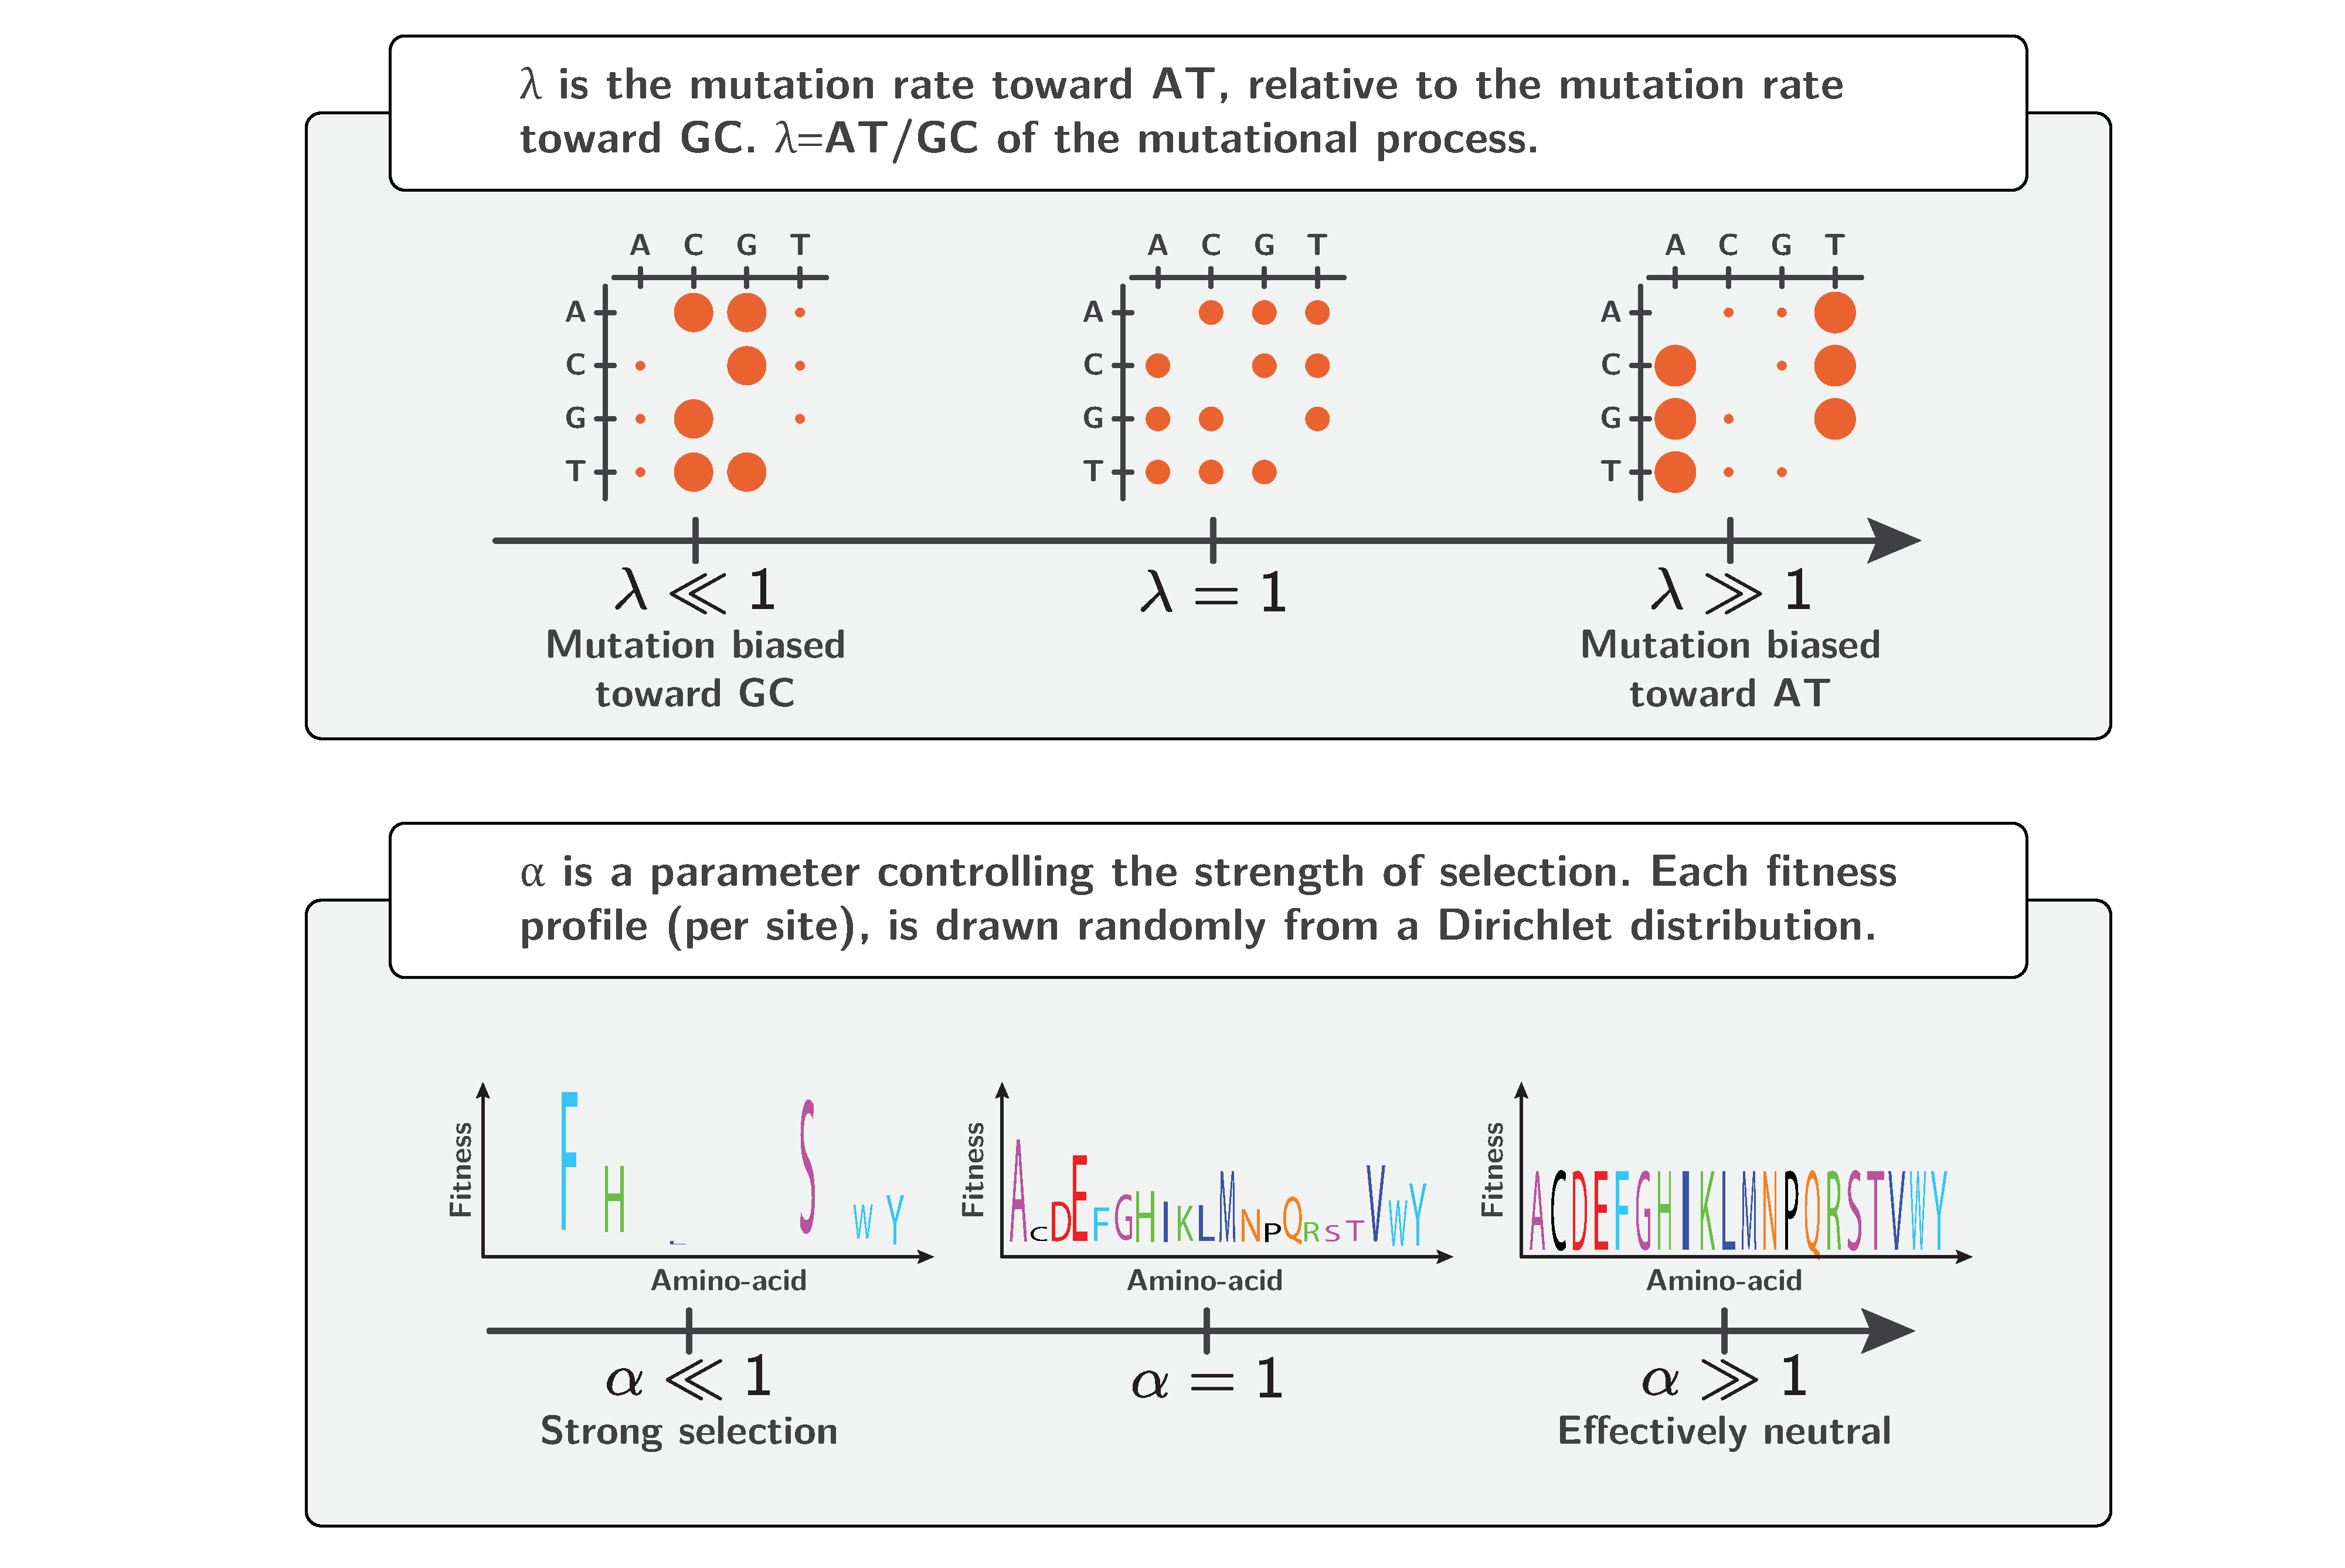
\includegraphics[width=\textwidth] {figures/mut-bias-parameters}
	\end{center}
	\caption[Parameters of the mutation-selection model]{Parameters of the mutation-selection model. One parameter for mutational bias, and one for strength of selection.}
\end{figure}

\begin{figure}[thbp]
	\begin{center}
		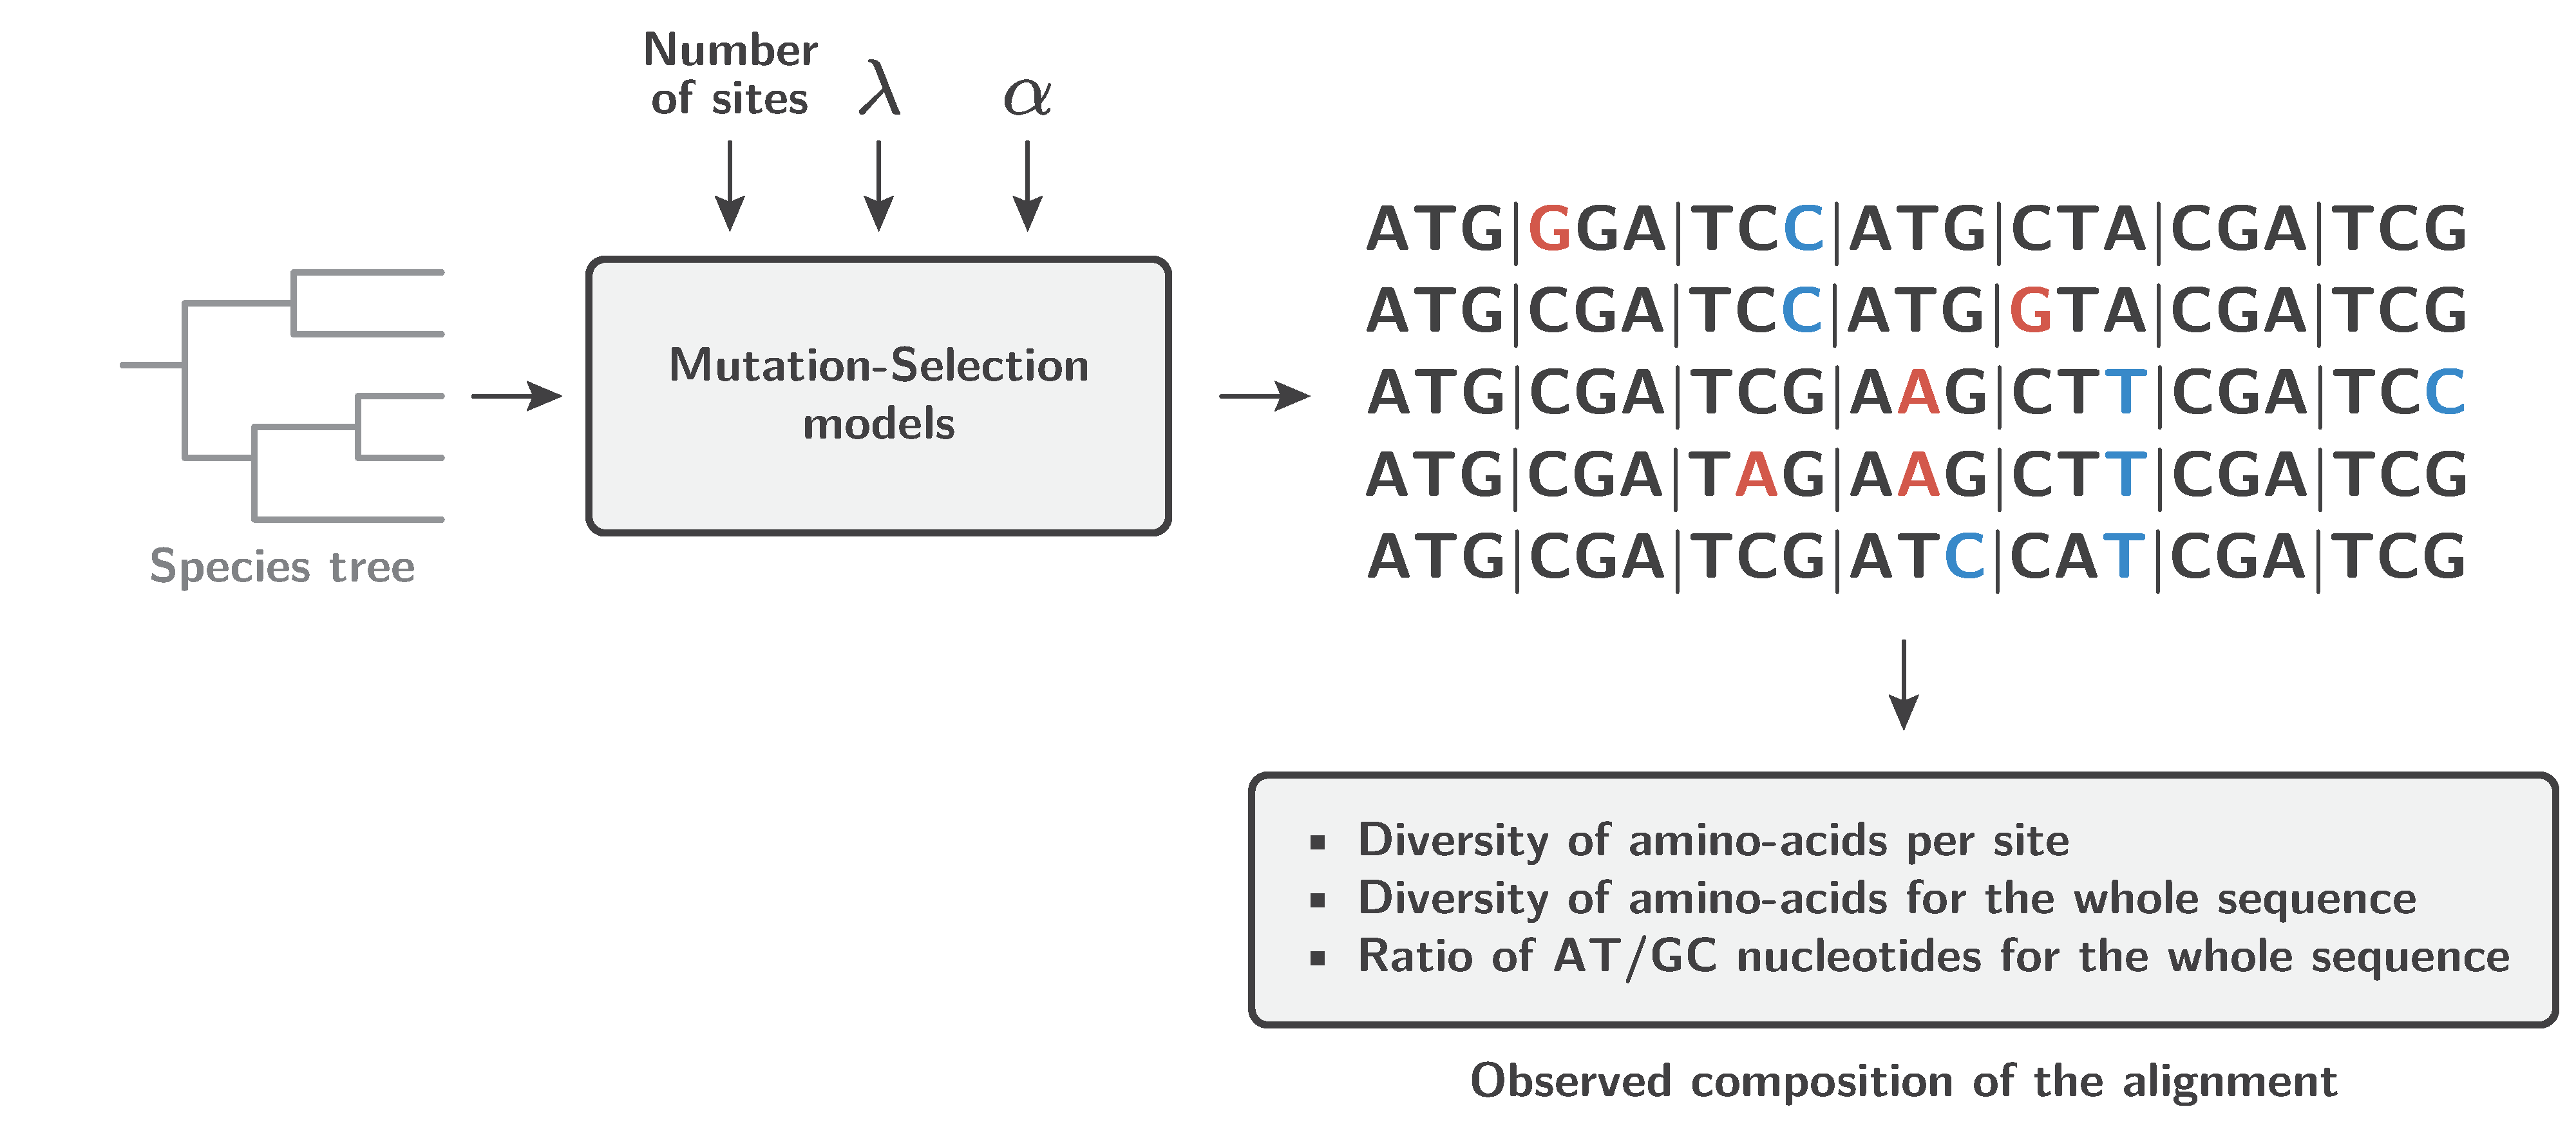
\includegraphics[width=\textwidth] {figures/mut-bias-simulations}
	\end{center}
	\caption[Simulations and analysis]{Simulations and analysis. We can observe composition of the alignment as function of the mutation and selection parameters.}
\end{figure}

\subsection{AT/GC as a function of the mutation-selection model}
The codon substitution process, at site $k$, which takes into account mutation and selection, is a function of $\lambda$ and $F^{(k)}$. Moreover this process has stationary distribution $\pi^{(k)}$. From this equilibrium frequency of codons, we define $\mathrm{AT_{obs}}^{(k)}(\lambda, F^{(k)})$ as the observed stationary distribution of weak nucleotides at site $k$:
\begin{align}
\mathrm{AT_{obs}}^{(k)}(\lambda, F^{(k)})
& =\frac{1}{3} \sum_{x \in \SetCodon} \Pi_x^{(k)} w_x , \ \textrm{by definition},\\
& =\frac{A^{(k)}}{3} \sum_{x \in \SetCodon} \lambda^{w_x} \e^{F_X^{(k)}} w_x , \ \textrm{from eq.} \ \ref{codonStationarity}.
\label{atPctSite}
\end{align}
As noted in \ref{sec:mutBias}, the mutational process leads to $(\pi_A+\pi_T)/(\pi_C+\pi_G) = \lambda$. Similarly, we denote the observed ratio of weak over strong nucleotide frequency, at site $k$, as $\lambda_{\mathrm{obs}}^{(k)} (\lambda, F^{(k)})$:
\begin{align}
\lambda_{\mathrm{obs}}^{(k)} (\lambda, F^{(k)})
& =\dfrac{\mathrm{AT_{obs}}^{(k)}(\lambda, F^{(k)})}{1 - \mathrm{AT_{obs}}^{(k)}(\lambda, F^{(k)}) }, \ \textrm{by definition},\\
& =\dfrac{ \sum_{x \in \SetCodon} \lambda^{w_x} \e^{F_X^{(k)}} w_x}{\sum_{x \in \SetCodon} \lambda^{w_x} \e^{F_X^{(k)}} (3 - w_x )}, \ \textrm{from eq.} \ \ref{atPctSite}.
\end{align}
At the sequence level, $\mathrm{AT_{obs}}(\lambda, \bm{F})$ is the observed stationary distribution of weak nucleotides:
\begin{align}
\mathrm{AT_{obs}}(\lambda, \bm{F})
& =\frac{1}{n}\sum_{k=1}^{n} \mathrm{AT_{obs}}^{(k)}(\lambda, F^{(k)}), \ \textrm{by definition}, \\
& =\frac{1}{3n}\sum_{k=1}^{n} \sum_{x \in \SetCodon} A^{(k)} \lambda^{w_x} \e^{F_X^{(k)}} w_x , \ \textrm{from eq.} \ \ref{atPctSite}.
\label{atPctSeq}
\end{align}
Similarly, we denote the observed ratio of weak over strong nucleotide frequency, for the whole sequence, as $\lambda_{\mathrm{obs}} (\lambda, \bm{F})$
\begin{align}
\lambda_{\mathrm{obs}} (\lambda, \bm{F})
& = \frac{\mathrm{AT_{obs}}(\lambda, \bm{F})}{ 1 - \mathrm{AT_{obs}}(\lambda, \bm{F}) }, \ \textrm{by definition},\\
& =\dfrac{ \sum_{k=1}^{n}  A^{(k)} \sum_{x \in \SetCodon} \lambda^{w_x} \e^{F_X^{(k)}} w_x}{ \sum_{k=1}^{n} A^{(k)} \sum_{x \in \SetCodon} \lambda^{w_x} \e^{F_X^{(k)}} (3 - w_x )}, \ \textrm{from eq.} \ \ref{atPctSeq}.
\end{align}
We then consider amino-acids propensities $S$ (exponential of fitnesses) as a multivariate continuous random variable. More specifically $S$ follow a Dirichlet distribution with concentration parameter $\alpha$.
\begin{equation}
S \sim \mathrm{Dirichlet}(\alpha, 20).
\end{equation}
Under a Dirichlet distribution of amino-acids propensities, the expected observed stationary distribution of weak nucleotides $\operatorname{E} [\mathrm{AT_{obs}}(\lambda, S)]$ is:
\begin{align}
\operatorname{E} [\mathrm{AT_{obs}}(\lambda, S)]
& =\int_{C(s)} \mathrm{AT_{obs}}(\lambda, s) p(s) \der s, \ \textrm{by defintion}, \\
& =\frac{1}{3} \int_{C(s)} A(\lambda, s) \sum_{x \in \SetCodon} 
\lambda^{w_x} s_X w_x p(s) \der s, \ \textrm{from eq.} \ \ref{atPctSite}, \\
& =\frac{1}{3} \int_{ C(s)} A(\lambda, s) \sum_{x \in \SetCodon}  \lambda^{w_x} s_X w_x {\frac {\Gamma (20 \alpha)}{\Gamma (\alpha )^{20}}} \prod_{Y \in \SetAa} s_Y^{\alpha-1} \der s, \\
& ={\frac {\Gamma (20 \alpha)}{3\Gamma (\alpha )^{20}}} \sum_{x \in \SetCodon} \lambda^{w_x} w_x  \int_{ C(s)} A(\lambda, s) s_X \prod_{Y \in \SetAa} s_Y^{\alpha-1} \der s, \\
& ={\frac {\Gamma (20 \alpha)}{3\Gamma (\alpha )^{20}}} \sum_{x \in \SetCodon} \lambda^{w_x} w_x \int_{ C(s)} s_X \dfrac{\prod_{Y \in \SetAa} s_Y^{\alpha-1}}{\sum_{y \in \SetCodon} \lambda^{w_y} s_Y} \der s, \\
& ={\frac {\Gamma (20 \alpha)}{3\Gamma (\alpha )^{20}}} \sum_{x \in \SetCodon} \lambda^{w_x} w_x \Phi_X(\lambda, \alpha),\\
&  \textrm{where} \  \Phi_X(\lambda, \alpha) = \int_{ C(s)} s_X \dfrac{\prod_{Y \in \SetAa} s_Y^{\alpha}}{\sum_{y \in \SetCodon} \lambda^{w_y} s_Y}\der s.
\label{atPctSeqExpected}
\end{align}
Similarly, the observed ratio of weak over strong nucleotide frequency, for the whole sequence, as $\operatorname{E} [\lambda_{\mathrm{obs}}(\lambda, S)]$: 
\begin{align}
\operatorname{E} [\lambda_{\mathrm{obs}}(\lambda, S)]
& =\frac{\operatorname{E} [\mathrm{AT_{obs}}(\lambda, S)]}{ 1 - \operatorname{E} [\mathrm{AT_{obs}}(\lambda, S)] }, \ \textrm{by definition},\\
& =\frac{\sum_{x \in \SetCodon} \lambda^{w_x} w_x \Phi_X(\lambda, \alpha)}{\sum_{x \in \SetCodon} \lambda^{w_x} (3 - w_x) \Phi_X(\lambda, \alpha)}, \ \textrm{from eq.} \ \ref{atPctSeqExpected}.
\label{atgcPctSeqExpected}
\end{align}
For a large sequence ($ n \gg 1 $), $\lambda_{\mathrm{obs}} (\lambda, \bm{F})$ converges to $\operatorname{E} [\lambda_{\mathrm{obs}}(\lambda, S)]$:
\begin{align}
\lambda_{\mathrm{obs}} (\lambda, \bm{F})
& \simeq \operatorname{E} [\lambda_{\mathrm{obs}}(\lambda, S)],\\
& =\frac{\sum_{x \in \SetCodon} \lambda^{w_x} w_x \Phi_X(\lambda, \alpha)}{\sum_{x \in \SetCodon} \lambda^{w_x} (3 - w_x) \Phi_X(\lambda, \alpha)}, \ \textrm{from eq.} \ \ref{atgcPctSeqExpected}.
\end{align}

\begin{figure}[thbp]
	\begin{center}
		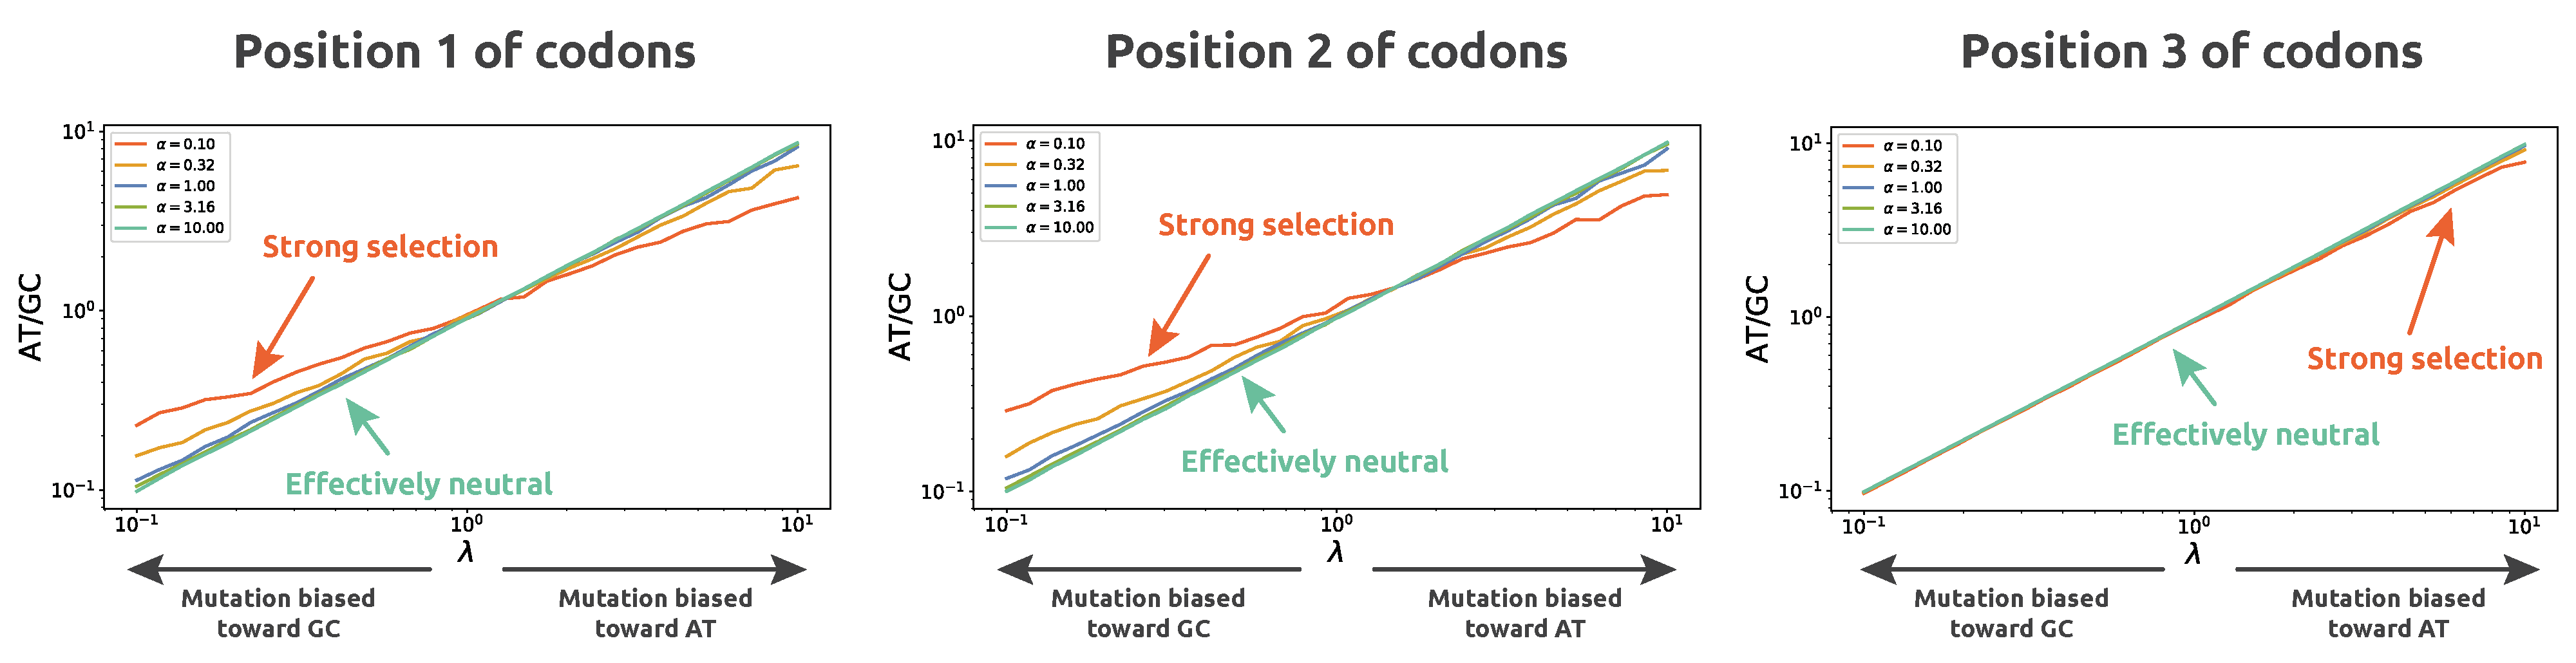
\includegraphics[width=\textwidth] {figures/mut-bias-AT-GC-obs}
	\end{center}
	\caption[AT/GC composition of the alignment]{AT/GC composition of the alignment. Observed AT/GC at the third codon position matches the mutational bias. Selection is balancing the mutational bias.}
\end{figure}

\subsection{Diversity of codons as a function of the mutation-selection model}

The evolutionary variability of an amino acid site in a protein family is an important indicator of the selective constraints that the site experiences. This variability is usually quantified either through the sequence entropy \citep{Goldstein2017}

Our analysis highlights how important it is to distinguish between amino acid frequencies averaged over a large class of sites with similar property (such as RSA) and amino acid frequencies at individual sites. In both cases, frequencies are Boltzmann distributed, and thus it is easy to mistake one for the other. However, the properties of these two distributions are very different. For example, in yeast, at sites with RSA close to 0.2 nearly all amino acids occur at comparable frequencies. Yet at any given site, only a small number ofamino acids are actually permissible. Evolutionary rate, which measures the rate at which mutations at individual sites arise and go to fixation, is governed by the amino acid distribution of individual sites, not the average distribution over a broad class of sites. \citep{Ramsey2011}

The codon substitution process, at site $k$, which takes into account mutation and selection, is a function of $\lambda$ and $F^{(k)}$. Moreover this process has stationary distribution $\pi^{(k)}$. From this equilibrium frequency of codons, we can compute the effective number of codon, mathematically this correspond to the diversity of the distribution $D^{(k)}$, at site $k$:
\begin{align}
D^{(k)}(\lambda, F^{(k)})
& =\e^{ - \sum_{x \in \SetCodon}  \Pi_x^{(k)} \ln ( \Pi_x^{(k)} )}, \ \textrm{by definition},\\
& =\e^{ - \sum_{x \in \SetCodon}  \Pi_x^{(k)} \ln \left( A^{(k)} \lambda^{w_x} \e^{F_X^{(k)}} \right)}, \ \textrm{from eq.} \ \ref{codonStationarity},\\
& =\e^{ - \sum_{x \in \SetCodon}  \Pi_x^{(k)} \left[ \ln ( A^{(k)} )+ \ln( \lambda^{w_x} ) + \ln (\e^{F_X^{(k)}}) \right] }\\
& =\e^{ - \ln ( A^{(k)} ) \sum_{x \in \SetCodon}  \Pi_x^{(k)} } \e^{ -  \ln (\lambda) \sum_{x \in \SetCodon}  \Pi_x^{(k)} w_x }\e^{ - \sum_{x \in \SetCodon}  \Pi_x^{(k)} F_X^{(k)}  } \\
& =\frac{1}{A^{(k)}} \e^{ -  \ln (\lambda) \sum_{x \in \SetCodon}  \Pi_x^{(k)} w_x }\e^{ - \sum_{x \in \SetCodon}  \Pi_x^{(k)} F_X^{(k)}  }
\label{entropy}
\end{align}

\begin{figure}[thbp]
	\begin{center}
		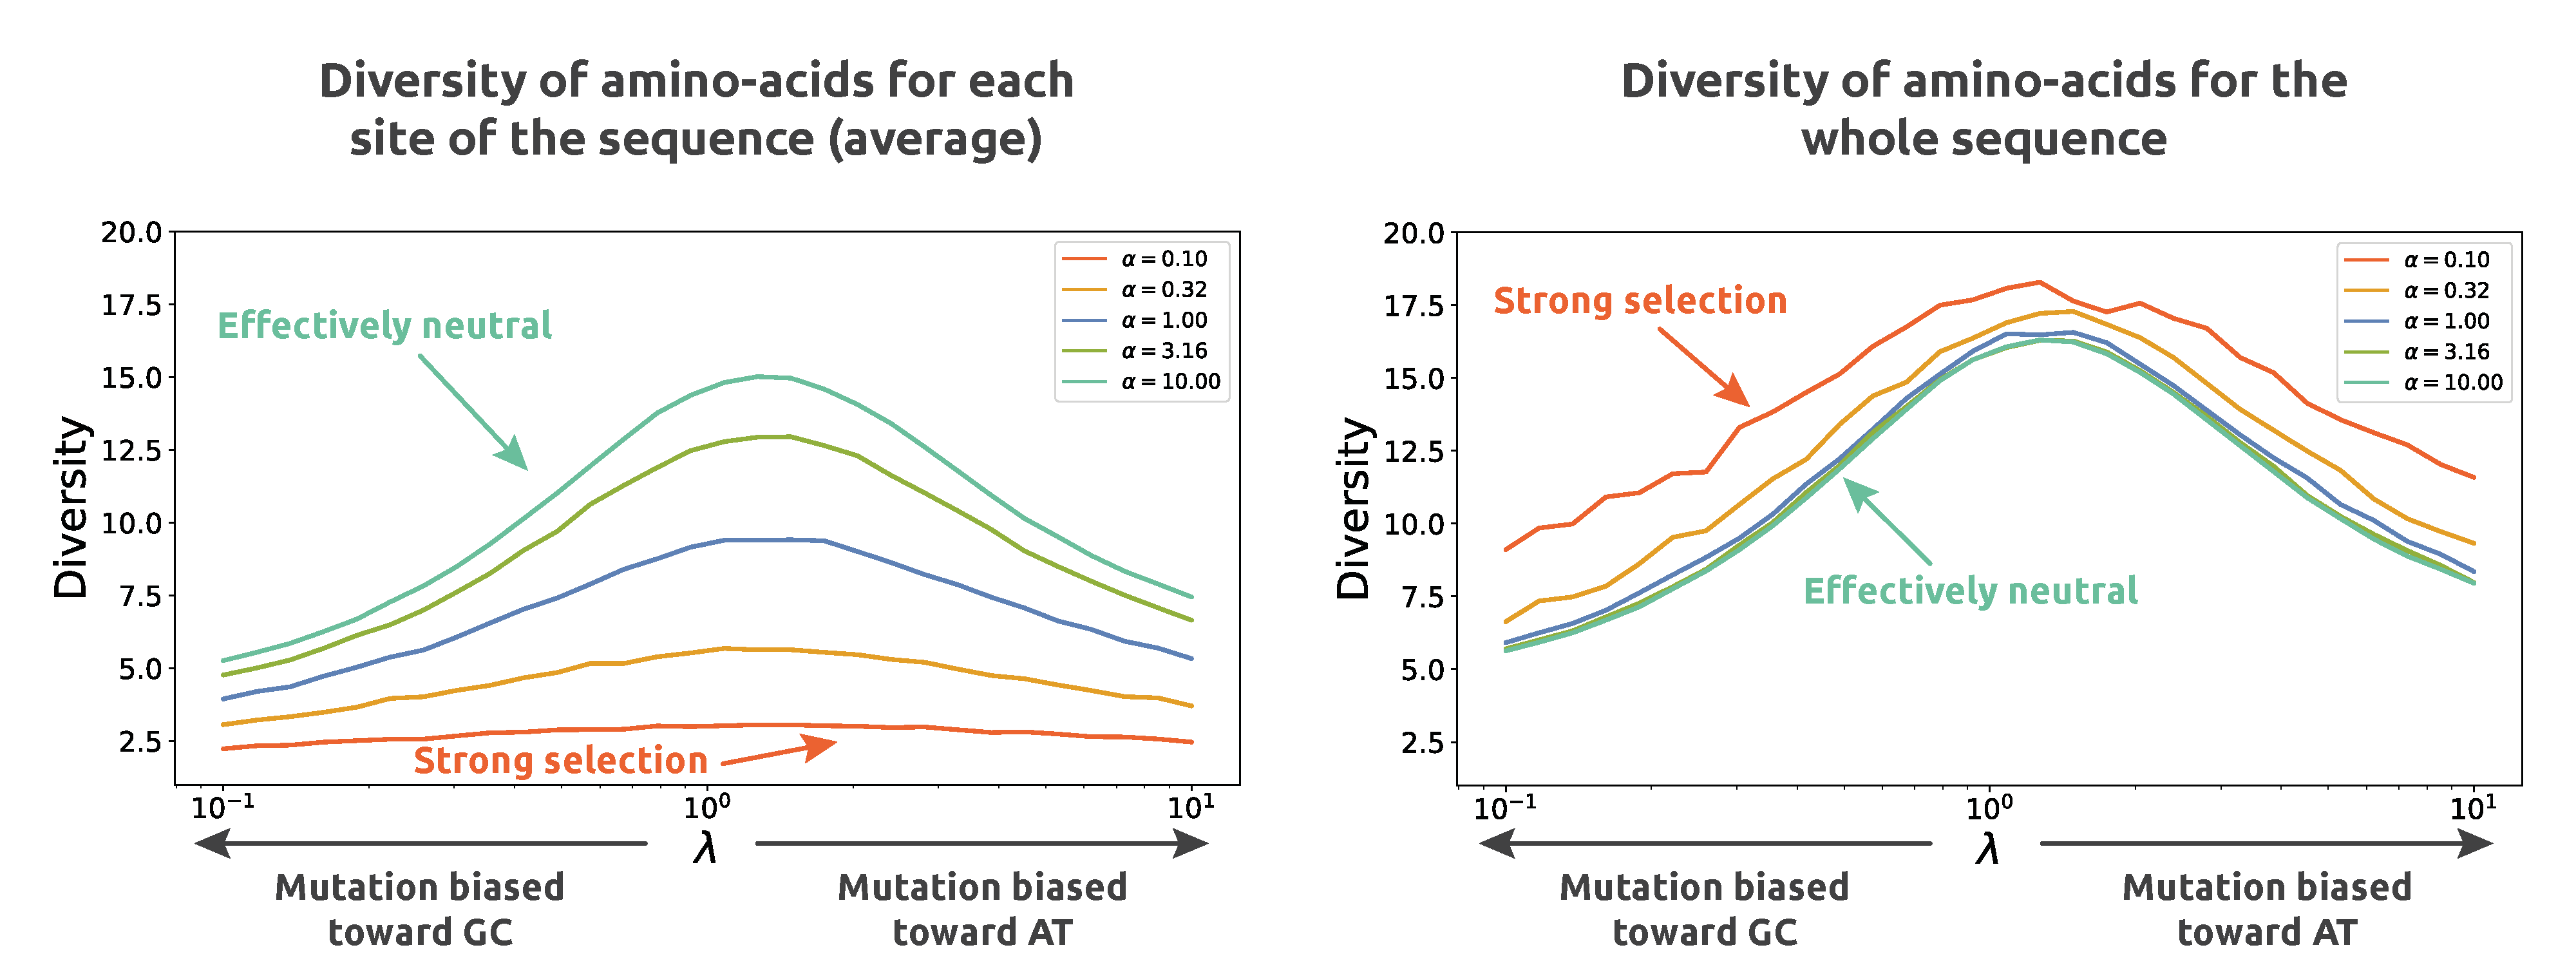
\includegraphics[width=\textwidth] {figures/mut-bias-diversity-aa}
	\end{center}
	\caption[Diversity of amino-acids]{Diversity of amino-acids. Sequence-diversity is higher than site-diversity. Diversity decreases with mutational bias.	Site-diversity decreases with selection. Sequence-diversity increase with selection.}
\end{figure}

\subsection{dN/dS as a function of the mutation-selection model}
The substitution rate (e.g., Grishin, Wolf \& Koonin, 2000). These two measures of evolutionary variability are considered to be essentially equivalent \citep{Halpern1998}, though they are differently influenced by the mutational process \citep{Santos2018}

The codon substitution process, at site $k$, which takes into account mutation and selection, is a function of $\lambda$ and $F^{(k)}$. Moreover this process has stationary distribution $\pi^{(k)}$. From this equilibrium frequency of codons, we define $L_{\NonSyn}^{(k)}(\lambda, F^{(k)})$ as the non-synonymous substitution flow, at site $k$:
\begin{align}
L_{\NonSyn}^{(k)}(\lambda, F^{(k)})
& =  \sum_{x \in \SetCodon} \sum_{y \in \NxNonSyn} \Pi_x^{(k)} Q_{x, y}^{(k)}, \ \textrm{by definition},\\
& =\sum_{x \in \SetCodon} \sum_{y \in \NxNonSyn} A^{(k)} \lambda^{w_x} \e^{F_X^{(k)}} U_{x, y} \dfrac{F_Y^{(k)} - F_X^{(k)}}{1 - \e^{F_X^{(k)} - F_Y^{(k)}}}, \ \textrm{from eq.}\ \ref{codonSubRates} \ \text{and} \ \ref{codonStationarity},\\
& =A^{(k)} \sum_{x \in \SetCodon} \lambda^{w_x} \sum_{y \in \NxNonSyn}  U_{x, y} \dfrac{F_Y^{(k)} - F_X^{(k)}}{\e^{-F_X^{(k)}} - \e^{ - F_Y^{(k)}}}.
\label{subFlowNonSyn}
\end{align}
Moreover, we define $K_{\NonSyn}^{(k)}(\lambda, F^{(k)})$ as the non-synonymous mutation flow, at site $k$:
\begin{align}
K_{\NonSyn}^{(k)}(\lambda, F^{(k)})
& =  \sum_{x \in \SetCodon} \sum_{y \in \NxNonSyn} \Pi_x^{(k)} U_{x, y}, \ \textrm{by definition},\\
& = A^{(k)}  \sum_{x \in \SetCodon} \lambda^{w_x} \sum_{y \in \NxNonSyn} \e^{F_X^{(k)}} U_{x, y}, \ \textrm{from eq.}\ \ref{codonSubRates} \ \text{and} \ \ref{codonStationarity}.
\label{mutFlowNonSyn}
\end{align}
We also define the mutation and substitution synonymous as $K_{\Syn}^{(k)}(\lambda, F^{(k)})$ and $L_{\Syn}^{(k)}(\lambda, F^{(k)})$ respectively:
\begin{align}
L_{\Syn}^{(k)}(\lambda, F^{(k)})
& =  \sum_{x \in \SetCodon} \sum_{y \in \NxSyn} \Pi_x^{(k)} Q_{x, y}^{(k)}, \ \textrm{by definition},\\
& =\sum_{x \in \SetCodon} \sum_{y \in \NxSyn} A^{(k)} \lambda^{w_x} \e^{F_X^{(k)}} U_{x, y}, \ \textrm{from eq.}\ \ref{codonSubRates} \ \text{and} \ \ref{codonStationarity}, \\
& =K_{\Syn}^{(k)}(\lambda, F^{(k)})
\label{subFlowSyn}
\end{align}
Following Spielman and Wilke \citep{Spielman2015}, the rate of non-synonymous to synonymous substitution is thus :
\begin{align}
\omega^{(k)}(\lambda, F^{(k)})
& =\dfrac{L_{\NonSyn}^{(k)}(\lambda, F^{(k)})}{K_{\NonSyn}^{(k)}(\lambda, F^{(k)})}  \left( \dfrac{L_{\Syn}^{(k)}(\lambda, F^{(k)})}{K_{\Syn}^{(k)}(\lambda, F^{(k)})}  \right)^{-1}, \\
& =\dfrac{L_{\NonSyn}^{(k)}(\lambda, F^{(k)})}{K_{\NonSyn}^{(k)}(\lambda, F^{(k)})}, \ \textrm{from eq.}\ \ref{subFlowSyn} \\
& =\dfrac{ \sum_{x \in \SetCodon} \lambda^{w_x} \sum_{y \in \NxNonSyn}  U_{x, y} \dfrac{F_Y^{(k)} - F_X^{(k)}}{\e^{ - F_Y^{(k)}} -  \e^{- F_X^{(k)}} } }{ \sum_{x \in \SetCodon}  \lambda^{w_x} \sum_{y \in \NxNonSyn} U_{x, y} \e^{F_X^{(k)}} }, \ \textrm{from eq.}\ \ref{subFlowNonSyn} \ \text{and} \ \ref{mutFlowNonSyn}.
\label{omegaSite}
\end{align}
The non-synonymous over synonymous rate for the whole sequence is then given by:
\begin{align}
\omega(\lambda, \bm{F})
& =\dfrac{\sum_{k=1}^{n} L_{\NonSyn}^{(k)}(\lambda, F^{(k)})}{\sum_{k=1}^{n}K_{\NonSyn}^{(k)}(\lambda, F^{(k)})}  \left( \dfrac{\sum_{k=1}^{n}L_{\Syn}^{(k)}(\lambda, F^{(k)})}{\sum_{k=1}^{n}K_{\Syn}^{(k)}(\lambda, F^{(k)})}  \right)^{-1}, \\
& =\dfrac{\sum_{k=1}^{n} L_{\NonSyn}^{(k)}(\lambda, F^{(k)})}{\sum_{k=1}^{n}K_{\NonSyn}^{(k)}(\lambda, F^{(k)})}, \ \textrm{from eq.}\ \ref{subFlowSyn} \\
& =\dfrac{ \sum_{k=1}^{n} \sum_{x \in \SetCodon} \lambda^{w_x} \sum_{y \in \NxNonSyn}  U_{x, y} \dfrac{F_Y^{(k)} - F_X^{(k)}}{\e^{ - F_Y^{(k)}} -  \e^{- F_X^{(k)}} } }{ \sum_{k=1}^{n} \sum_{x \in \SetCodon}  \lambda^{w_x}  \sum_{y \in \NxNonSyn} U_{x, y} \e^{F_X^{(k)}}}, \ \textrm{from eq.}\ \ref{subFlowNonSyn} \ \text{and} \ \ref{mutFlowNonSyn}. \\
& =\dfrac{ \sum_{x \in \SetCodon} \lambda^{w_x} \sum_{y \in \NxNonSyn}  U_{x, y}  \sum_{k=1}^{n} \dfrac{F_Y^{(k)} - F_X^{(k)}}{\e^{ - F_Y^{(k)}} -  \e^{- F_X^{(k)}} } }{  \sum_{x \in \SetCodon}  \lambda^{w_x}  \sum_{y \in \NxNonSyn} U_{x, y}  \sum_{k=1}^{n} \e^{F_X^{(k)}}}.
\label{omegaSeq}
\end{align}
We then consider amino-acids propensities $S$ (exponential of fitnesses) as a multivariate continuous random variable. More specifically $S$ follow a Dirichlet distribution with concentration parameter $\alpha$.
\begin{equation}
S \sim \mathrm{Dirichlet}(\alpha, 20).
\end{equation}
Under a Dirichlet distribution of amino-acids propensities, the expected non-synonymous substitution flow $\operatorname{E} [L_{\NonSyn}(\lambda, S)]$ :
\begin{align}
\operatorname{E} [L_{\NonSyn}(\lambda, S)]
& =\int_{C(s)} L_{\NonSyn}(\lambda, s) p(s) \der s, \ \textrm{by defintion}, \\
& =\int_{C(s)} A(\lambda, s) \sum_{x \in \SetCodon} \lambda^{w_x} \sum_{y \in \NxNonSyn} U_{x, y} s_X s_Y\dfrac{\ln(s_Y)-\ln(s_X)}{s_Y - s_Y} p(s) \der s , \ \textrm{from eq.}\ \ref{subFlowNonSyn}, \\
& =\int_{C(s)} A(\lambda, s) \sum_{x \in \SetCodon} \lambda^{w_x} \sum_{y \in \NxNonSyn} U_{x, y} s_X s_Y\dfrac{\ln(s_Y)-\ln(s_X)}{s_Y - s_Y} {\frac {\Gamma (20 \alpha)}{\Gamma (\alpha )^{20}}} \prod_{X \in \SetAa} s_X^{\alpha-1} \der s,\\
& ={\frac {\Gamma (20 \alpha)}{\Gamma (\alpha )^{20}}} \sum_{x \in \SetCodon} \lambda^{w_x} \sum_{y \in \NxNonSyn} U_{x, y} \int_{C(s)} s_Y\dfrac{\ln(s_Y)-\ln(s_X)}{s_Y - s_Y} \dfrac{\prod_{X \in \SetAa} s_X^{\alpha}}{\sum_{y \in \SetCodon} \lambda^{w_y} s_Y} \der s.\\
& ={\frac {\Gamma (20 \alpha)}{\Gamma (\alpha )^{20}}} \sum_{x \in \SetCodon} \lambda^{w_x} \sum_{y \in \NxNonSyn} U_{x, y} \Psi(\lambda, \alpha), \\
& \textrm{where} \ \Psi(\lambda, \alpha) = \int_{C(s)} s_Y\dfrac{\ln(s_Y)-\ln(s_X)}{s_Y - s_Y} \dfrac{\prod_{X \in \SetAa} s_X^{\alpha}}{\sum_{y \in \SetCodon} \lambda^{w_y} s_Y} \der s.
\end{align}
Moreover, the expected non-synonymous mutation flow $\operatorname{E} [K_{\NonSyn}(\lambda, S)]$ is:
\begin{align}
\operatorname{E} [K_{\NonSyn}(\lambda, S)]
& =  \int_{C(s)} K_{\NonSyn}(\lambda, s) p(s) \der s, \ \textrm{by defintion}, \\
& =\int_{C(s)} A(\lambda, s) \sum_{x \in \SetCodon} \lambda^{w_x} \sum_{y \in \NxNonSyn} s_X U_{x, y} p(s) \der s , \ \textrm{from eq.}\ \ref{mutFlowNonSyn}, \\
& =\int_{C(s)} A(\lambda, s) \sum_{x \in \SetCodon} \lambda^{w_x} \sum_{y \in \NxNonSyn} s_X U_{x, y}{\frac {\Gamma (20 \alpha)}{\Gamma (\alpha )^{20}}} \prod_{X \in \SetAa} s_X^{\alpha-1} \der s,\\
& =\frac{\Gamma (20 \alpha)}{\Gamma (\alpha )^{20}} \sum_{x \in \SetCodon} \lambda^{w_x} \sum_{y \in \NxNonSyn} U_{x, y} \int_{C(s)} \dfrac{\prod_{X \in \SetAa} s_X^{\alpha}}{\sum_{y \in \SetCodon} \lambda^{w_y} s_Y}\der s,\\
& =\frac{\Gamma (20 \alpha)}{\Gamma (\alpha )^{20}} \sum_{x \in \SetCodon} \lambda^{w_x} \sum_{y \in \NxNonSyn} U_{x, y} \Phi(\lambda, \alpha).\\
\end{align}
The expected non-synonymous over synonymous rate, $\operatorname{E} [\omega(\lambda, S)]$ , is then given by:
\begin{align}
\operatorname{E} [\omega(\lambda, S)]
& =  \dfrac{\operatorname{E} [L_{\NonSyn}(\lambda, S)]}{\operatorname{E} [K_{\NonSyn}(\lambda, S)]} \\
& =\dfrac{\sum_{x \in \SetCodon} \lambda^{w_x} \sum_{y \in \NxNonSyn} U_{x, y} \Psi(\lambda, \alpha)}{\sum_{x \in \SetCodon} \lambda^{w_x} \sum_{y \in \NxNonSyn} U_{x, y} \Phi(\lambda, \alpha)}.
\label{omegaExpected}
\end{align}
For a large sequence ($ n \gg 1 $), $\omega (\lambda, \bm{F})$ converges to $\operatorname{E} [\omega(\lambda, S)]$:
\begin{align}
\omega (\lambda, \bm{F})
& \simeq \operatorname{E} [\omega(\lambda, S)],\\
& =\dfrac{\sum_{x \in \SetCodon} \lambda^{w_x} \sum_{y \in \NxNonSyn} U_{x, y} \Psi(\lambda, \alpha)}{\sum_{x \in \SetCodon} \lambda^{w_x} \sum_{y \in \NxNonSyn} U_{x, y} \Phi(\lambda, \alpha)}, \ \textrm{from eq.} \ \ref{omegaExpected}.
\end{align}

\begin{figure}[thbp]
	\begin{center}
		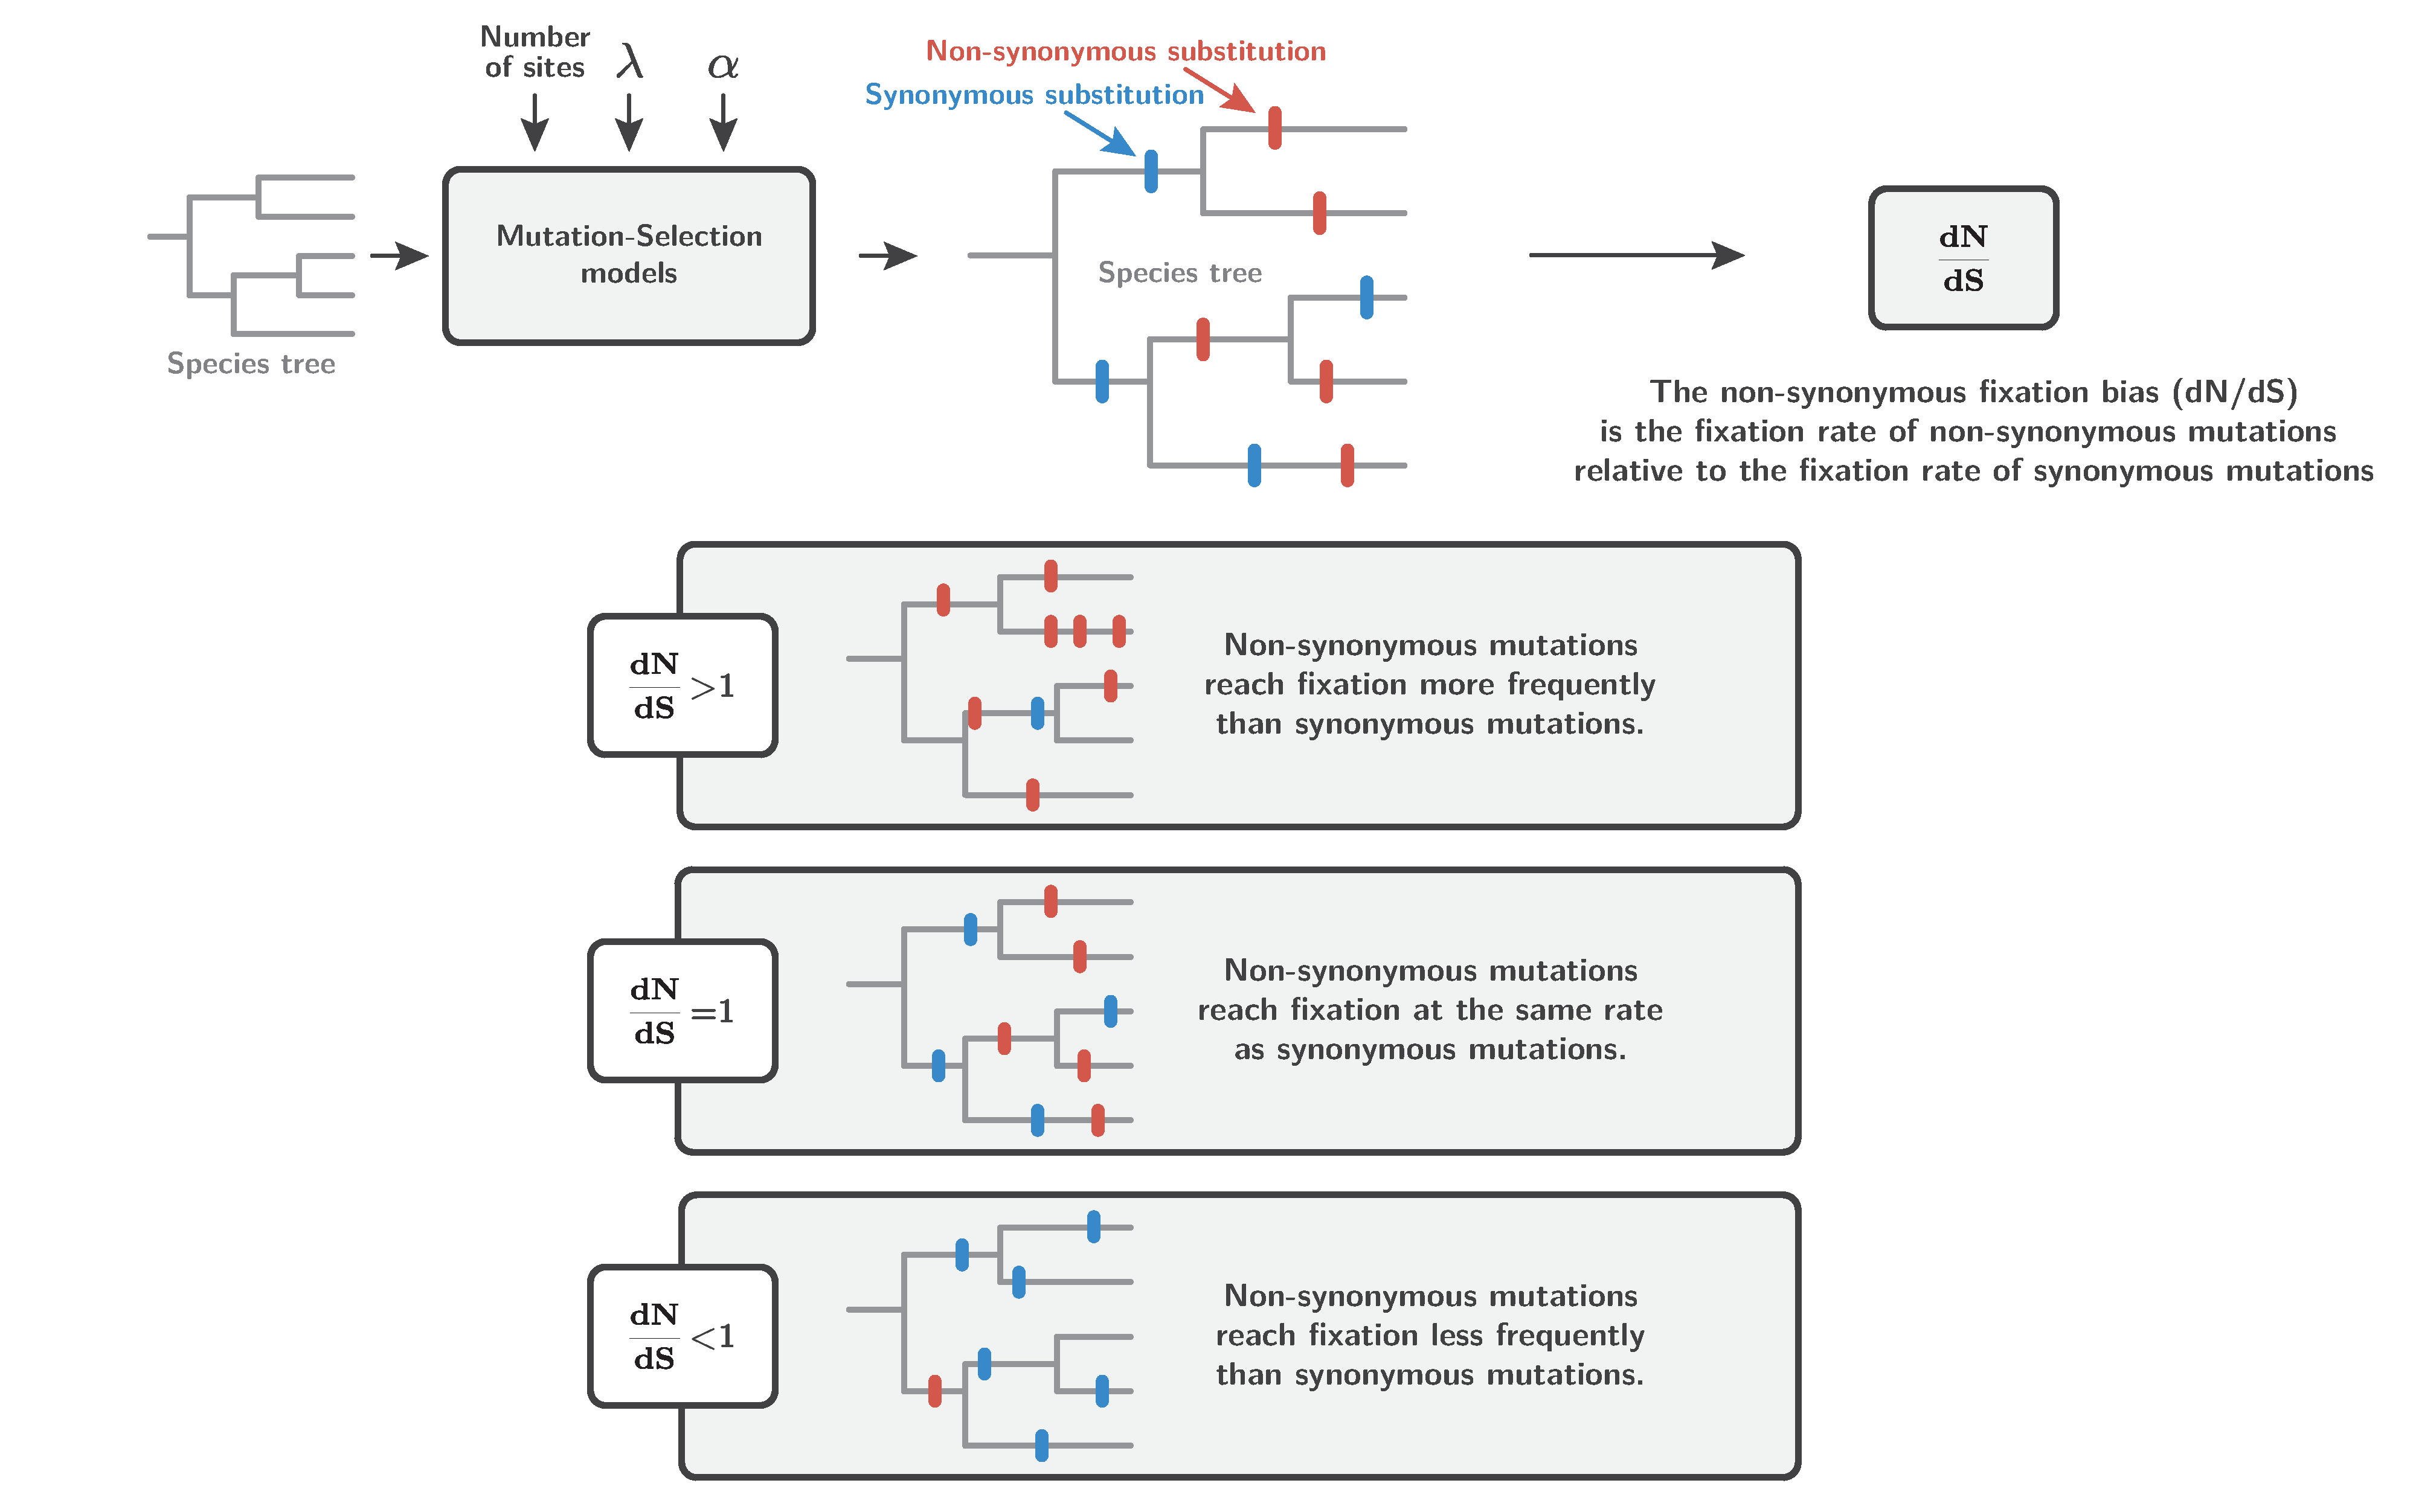
\includegraphics[width=\textwidth] {figures/mut-bias-definitions}
	\end{center}
	\caption[Definition of $\omega$]{Definition of $\omega$.}
\end{figure}

\begin{figure}[thbp]
	\begin{center}
		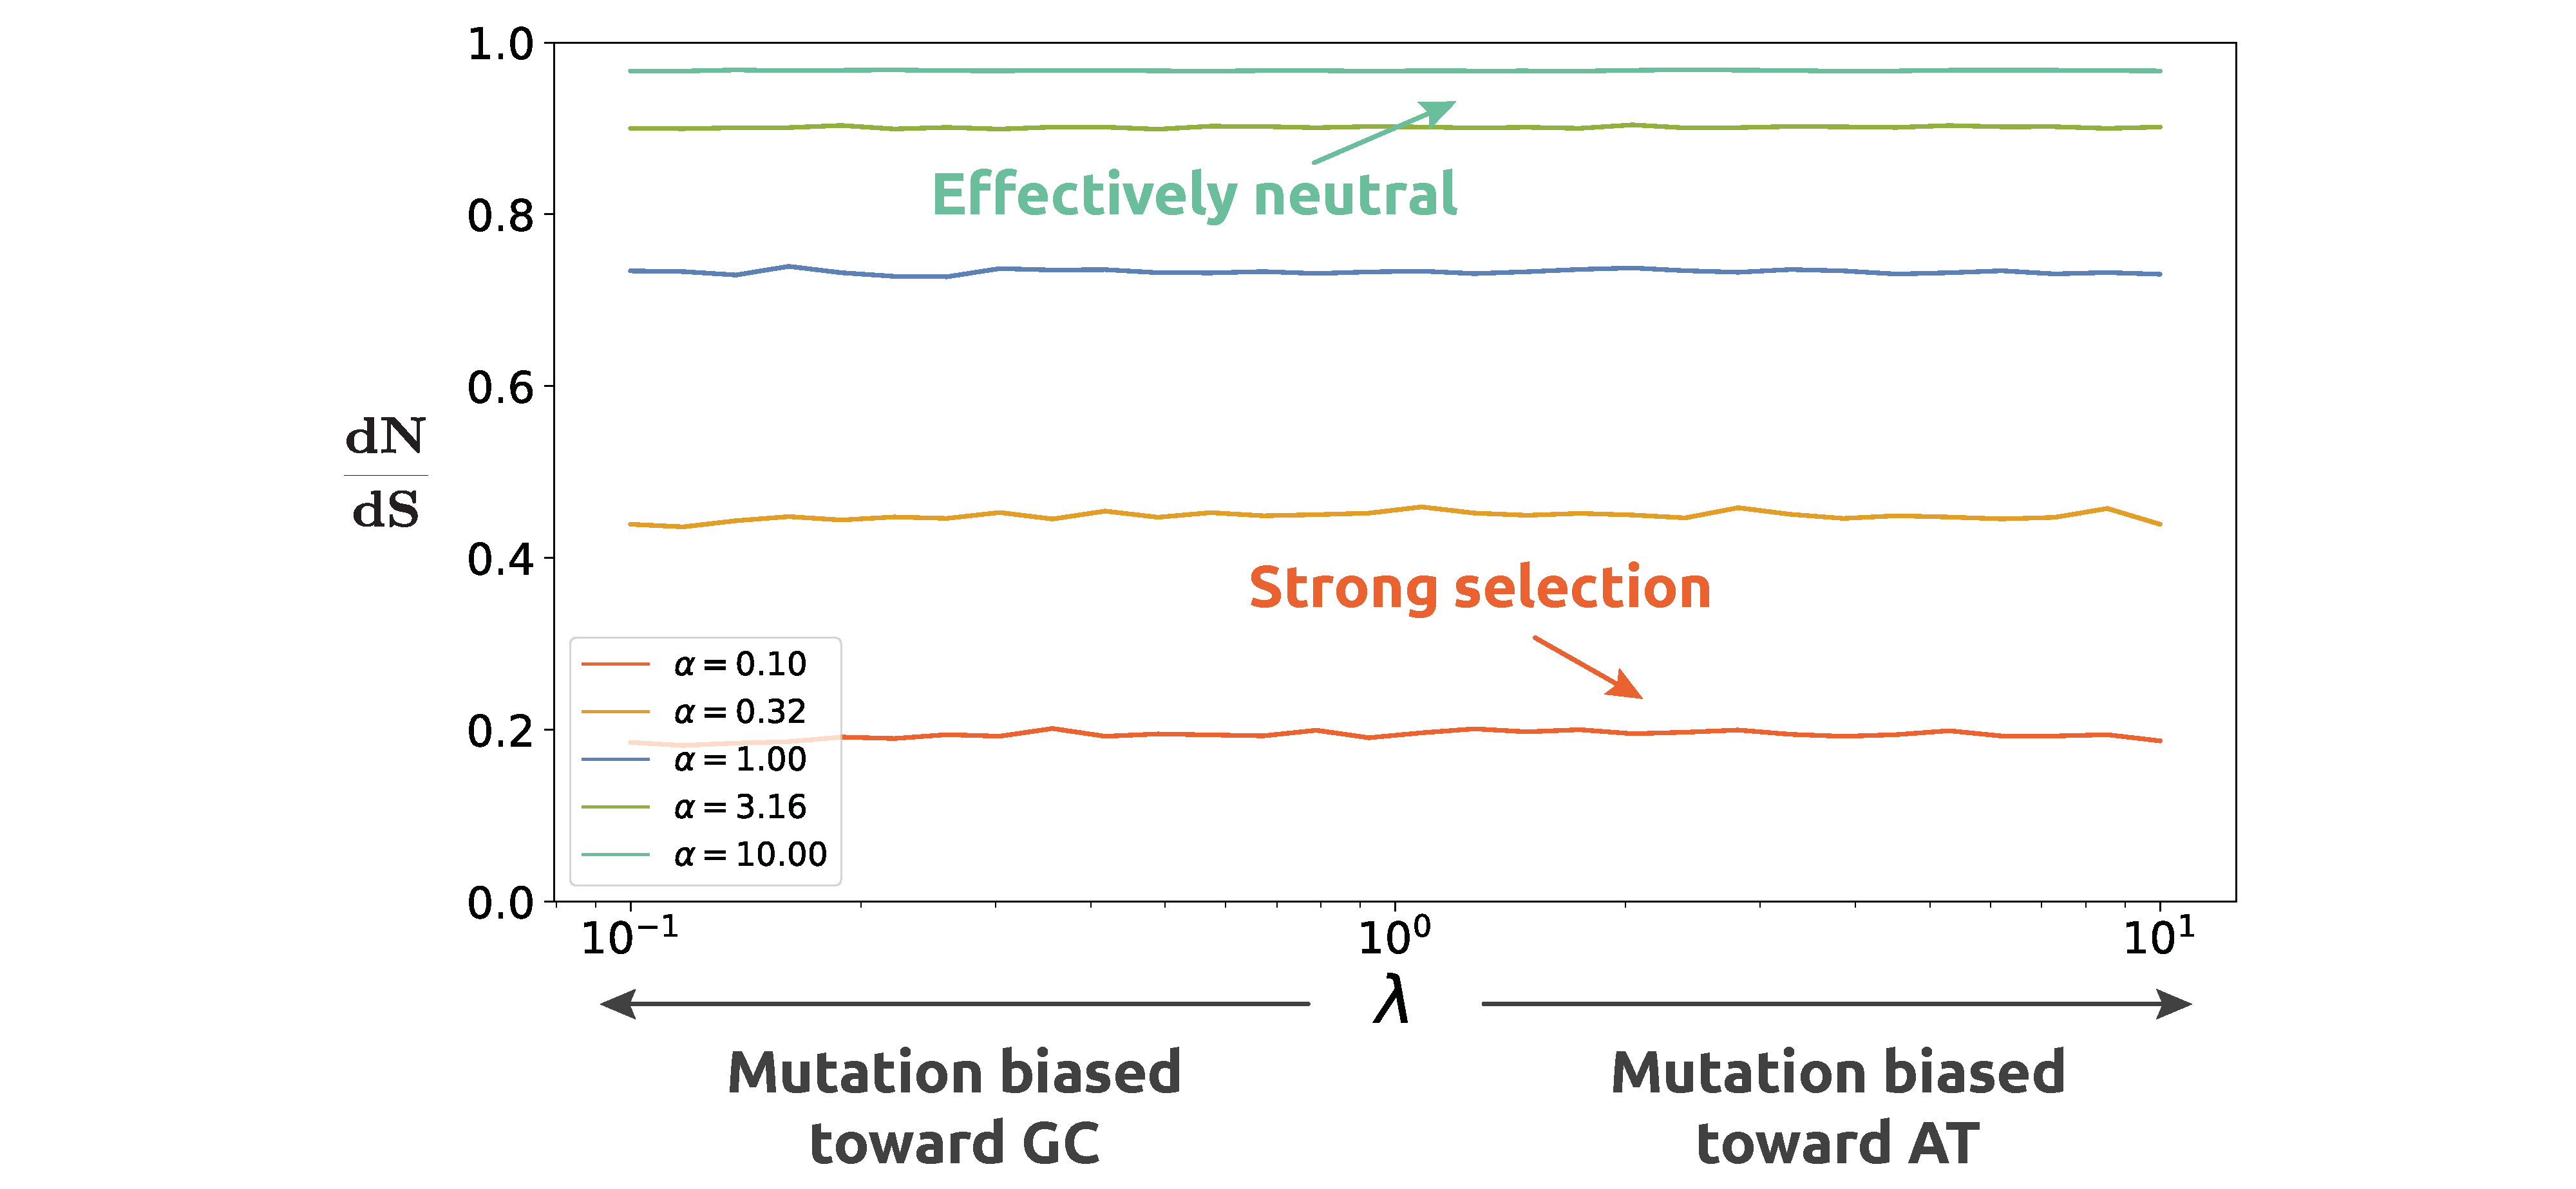
\includegraphics[width=\textwidth] {figures/mut-bias-omega}
	\end{center}
	\caption[$\omega$ as a function of the parameters]{$\omega$ as a function of the parameters. Non-synonymous fixation bias is always lower than. Non-synonymous fixation bias decrease with the strength of selection. Non-synonymous fixation bias is unaffected by mutational bias.}
\end{figure}

\begin{figure}[thbp]
	\begin{center}
		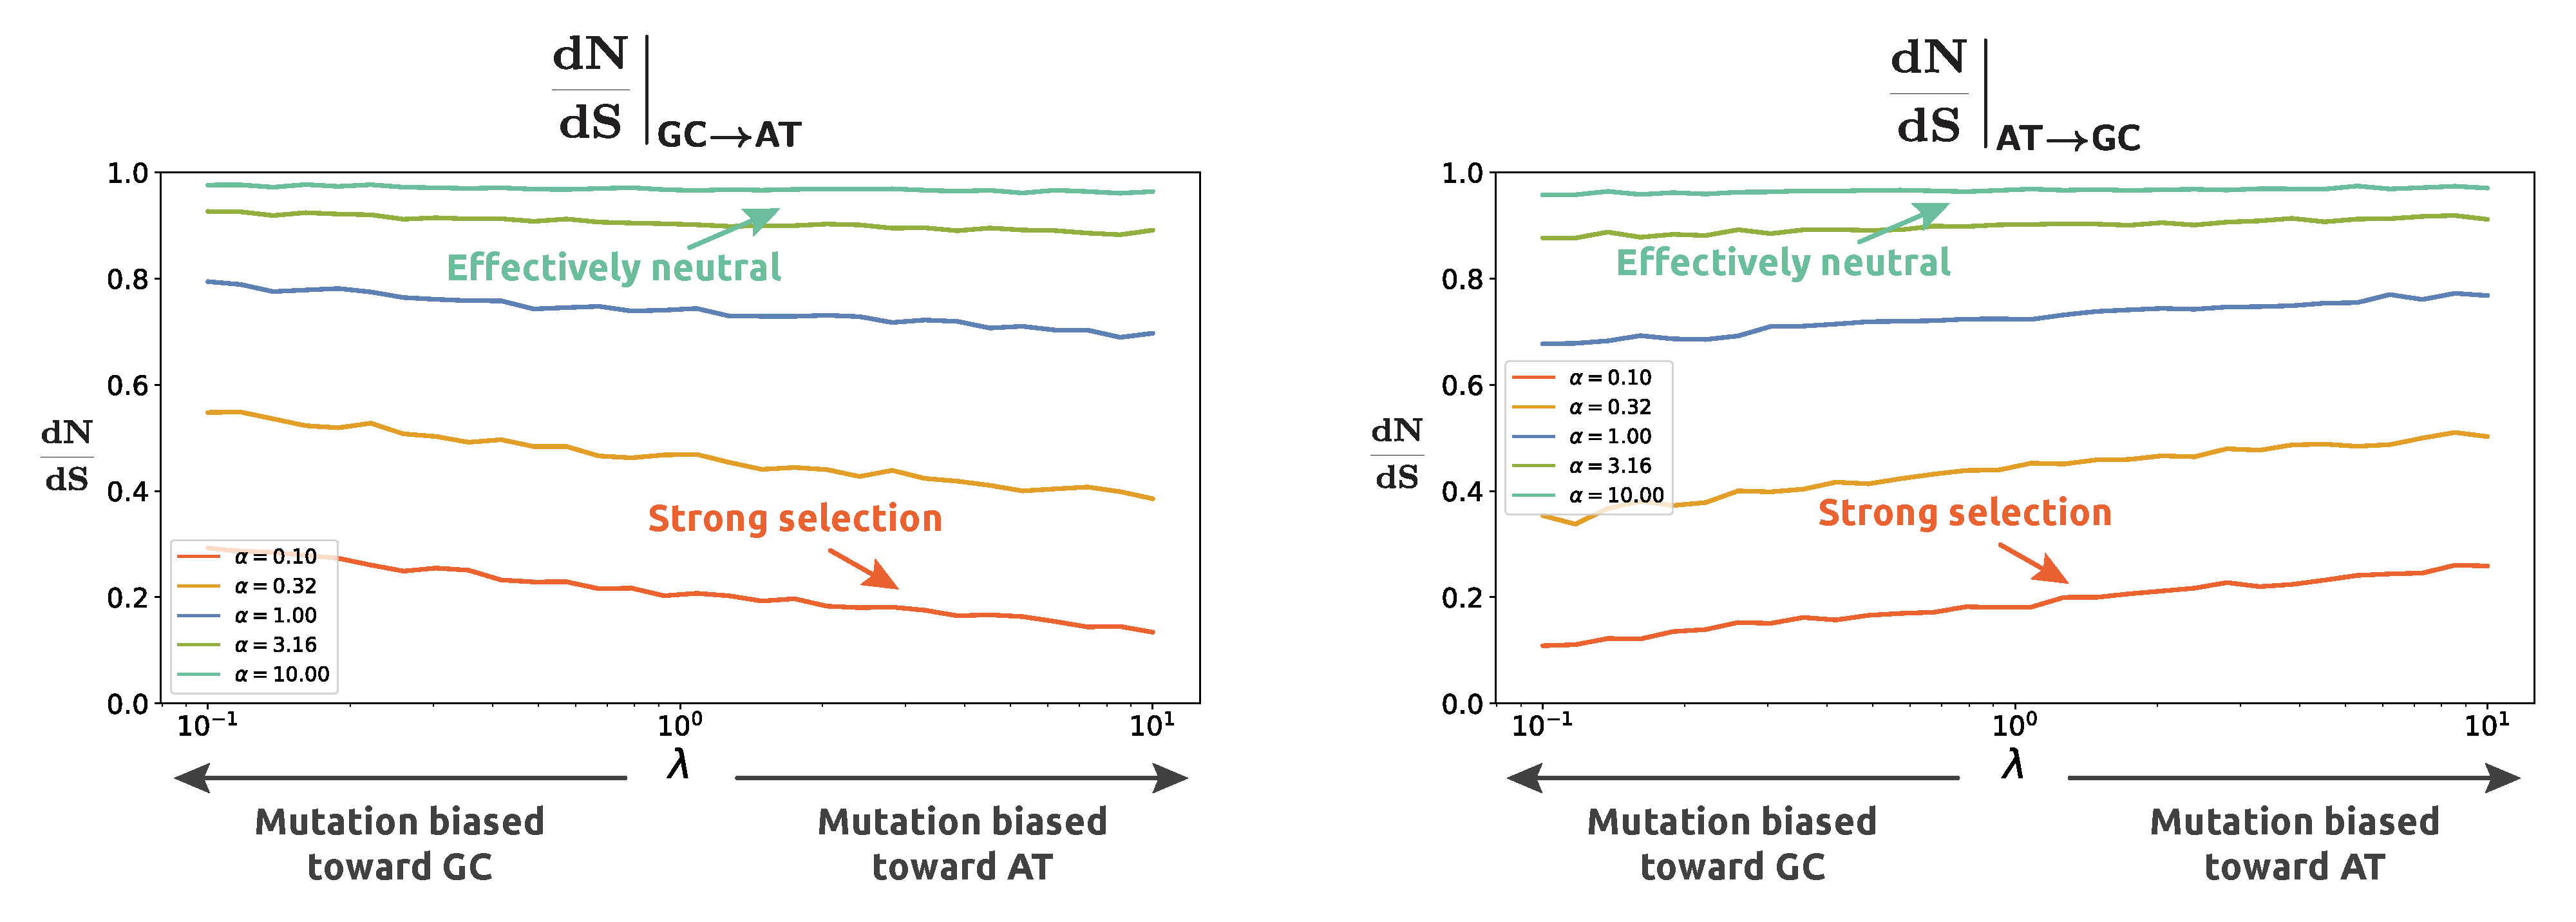
\includegraphics[width=\textwidth, page=1] {figures/mut-bias-omega-WS-SW}
	\end{center}
	\caption[Fixation bias of non-synonymous mutations]{Fixation bias of non-synonymous mutations. Mutation biased from GC to AT leads to a fixation bias in the opposite direction. More generally, mutation bias leads to balancing fixation bias. This is confounding factor with gBGC.}
\end{figure}

\section{Parametric inference}

\begin{figure}[thbp]
	\begin{center}
		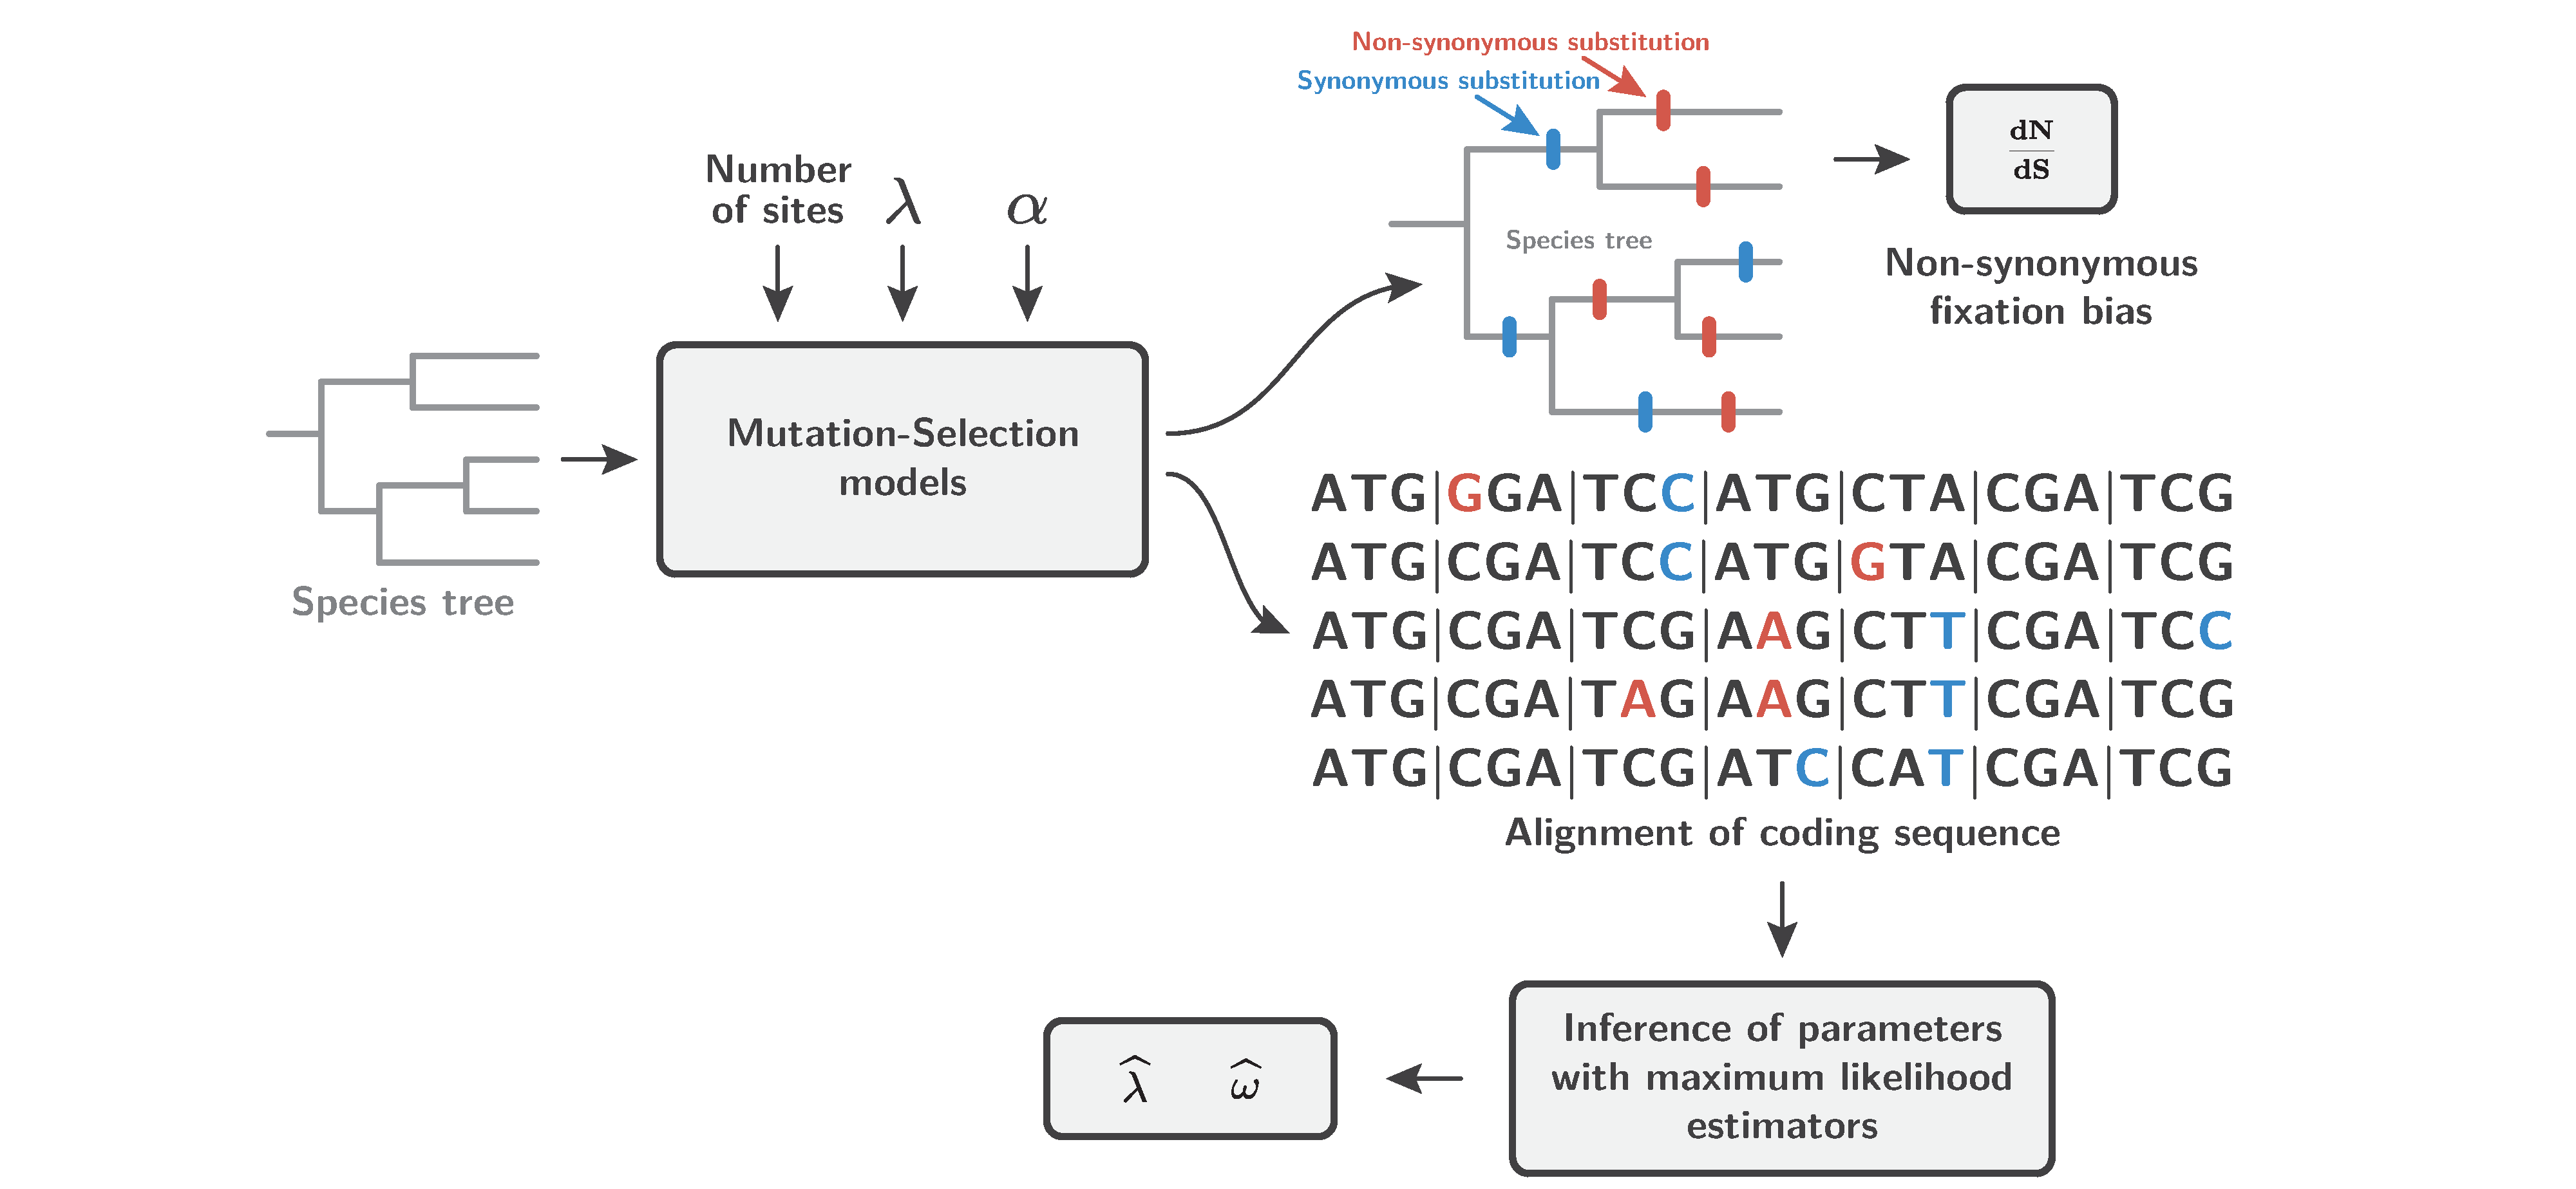
\includegraphics[width=\textwidth, page=1] {figures/mut-bias-pipeline}
	\end{center}
	\caption[Inferred value compared to known value]{Inferred value compared to known value.}
\end{figure}

\subsection{Parametric inference with Muse-Gaut model}

\begin{itemize}
	\item ${q_{{\color{RED}{\textbf{ATT}}} \rightarrow {\color{GREEN}\textbf{ATG}}}}$ is the substitution rate from codon ${\color{RED}{\textbf{ATT}}}$ to ${\color{GREEN}\textbf{ATG}}$.
	\item ${\mu_{{\color{RED}\textbf{T}} \rightarrow {\color{GREEN}\textbf{G}}}}$ is the mutation rate from nucleotide ${\color{RED}\textbf{T}}$ to ${\color{GREEN}\textbf{G}}$ 
	\item ${\omega}$ is the non-synonymous fixation bias. 
\end{itemize}
\begin{equation*}
\begin{dcases}
{q_{{\color{RED}{\textbf{ATT}}} \rightarrow {\color{GREEN}\textbf{ATG}}}} = { \omega \mu_{{\color{RED}\textbf{T}} \rightarrow {\color{GREEN}\textbf{G}}} } & \text{since } {\color{RED}{\textbf{ATT}}} \text{ and } {\color{GREEN}\textbf{ATG}} \text{ are non-synonymous} \\
{q_{{\color{RED}{\textbf{ATT}}} \rightarrow {\color{BLUE}\textbf{ATA}}}} = { \mu_{{\color{RED}\textbf{T}} \rightarrow {\color{BLUE}\textbf{A}}}} & \text{since } {\color{RED}{\textbf{ATT}}} \text{ and } {\color{BLUE}\textbf{ATA}} \text{ are synonymous}\\
\end{dcases}
\end{equation*}
From the maximum likelihood estimates of the $4 \times 4$ mutation matrix $\left({\widehat{\mu}} \right)$, we can estimate of the mutational bias toward $\mathrm{AT}$ $\left({\widehat{\lambda}_{\text{MG}}} \right)$. We can also estimate the fixation bias of non-synonymous mutations $\left({\widehat{\omega}_{\text{MG}}} \right)$


\subsection{Inference under projected mutation-selection}
\begin{itemize}
	\item ${\beta_{{\color{RED}{\textbf{Ile}}} \rightarrow {\color{GREEN}{\textbf{Met}}}}}$ is the fixation bias from Isoleucine to Methionine
\end{itemize}
\begin{equation*}
\begin{dcases}
{q_{{\color{RED}{\textbf{ATT}}} \rightarrow {\color{GREEN}\textbf{ATG}}}} = { \beta_{{\color{RED}{\textbf{Ile}}} \rightarrow {\color{GREEN}{\textbf{Met}}}} \mu_{{\color{RED}\textbf{T}} \rightarrow {\color{GREEN}\textbf{G}}}} & \text{since } {\color{RED}{\textbf{ATT}}} \text{ and } {\color{GREEN}\textbf{ATG}} \text{ are non-synonymous} \\
{q_{{\color{RED}{\textbf{ATT}}} \rightarrow {\color{BLUE}\textbf{ATA}}}} = {\mu_{{\color{RED}\textbf{T}} \rightarrow {\color{BLUE}\textbf{A}}} } & \text{since } {\color{RED}{\textbf{ATT}}} \text{ and } {\color{BLUE}\textbf{ATA}} \text{ are synonymous}\\
\end{dcases}
\end{equation*}
From the maximum likelihood estimates of the $4 \times 4$ mutation matrix $\left({\widehat{\mu}} \right)$, we can estimate the mutational bias $\mathrm{AT}$ $\left({\widehat{\lambda}_{\text{MF}}} \right)$. We can also estimate the fixation bias of non-synonymous mutations $\left({\widehat{\omega}_{\text{MF}}} \right)$


\begin{figure}[thbp]
	\begin{center}
		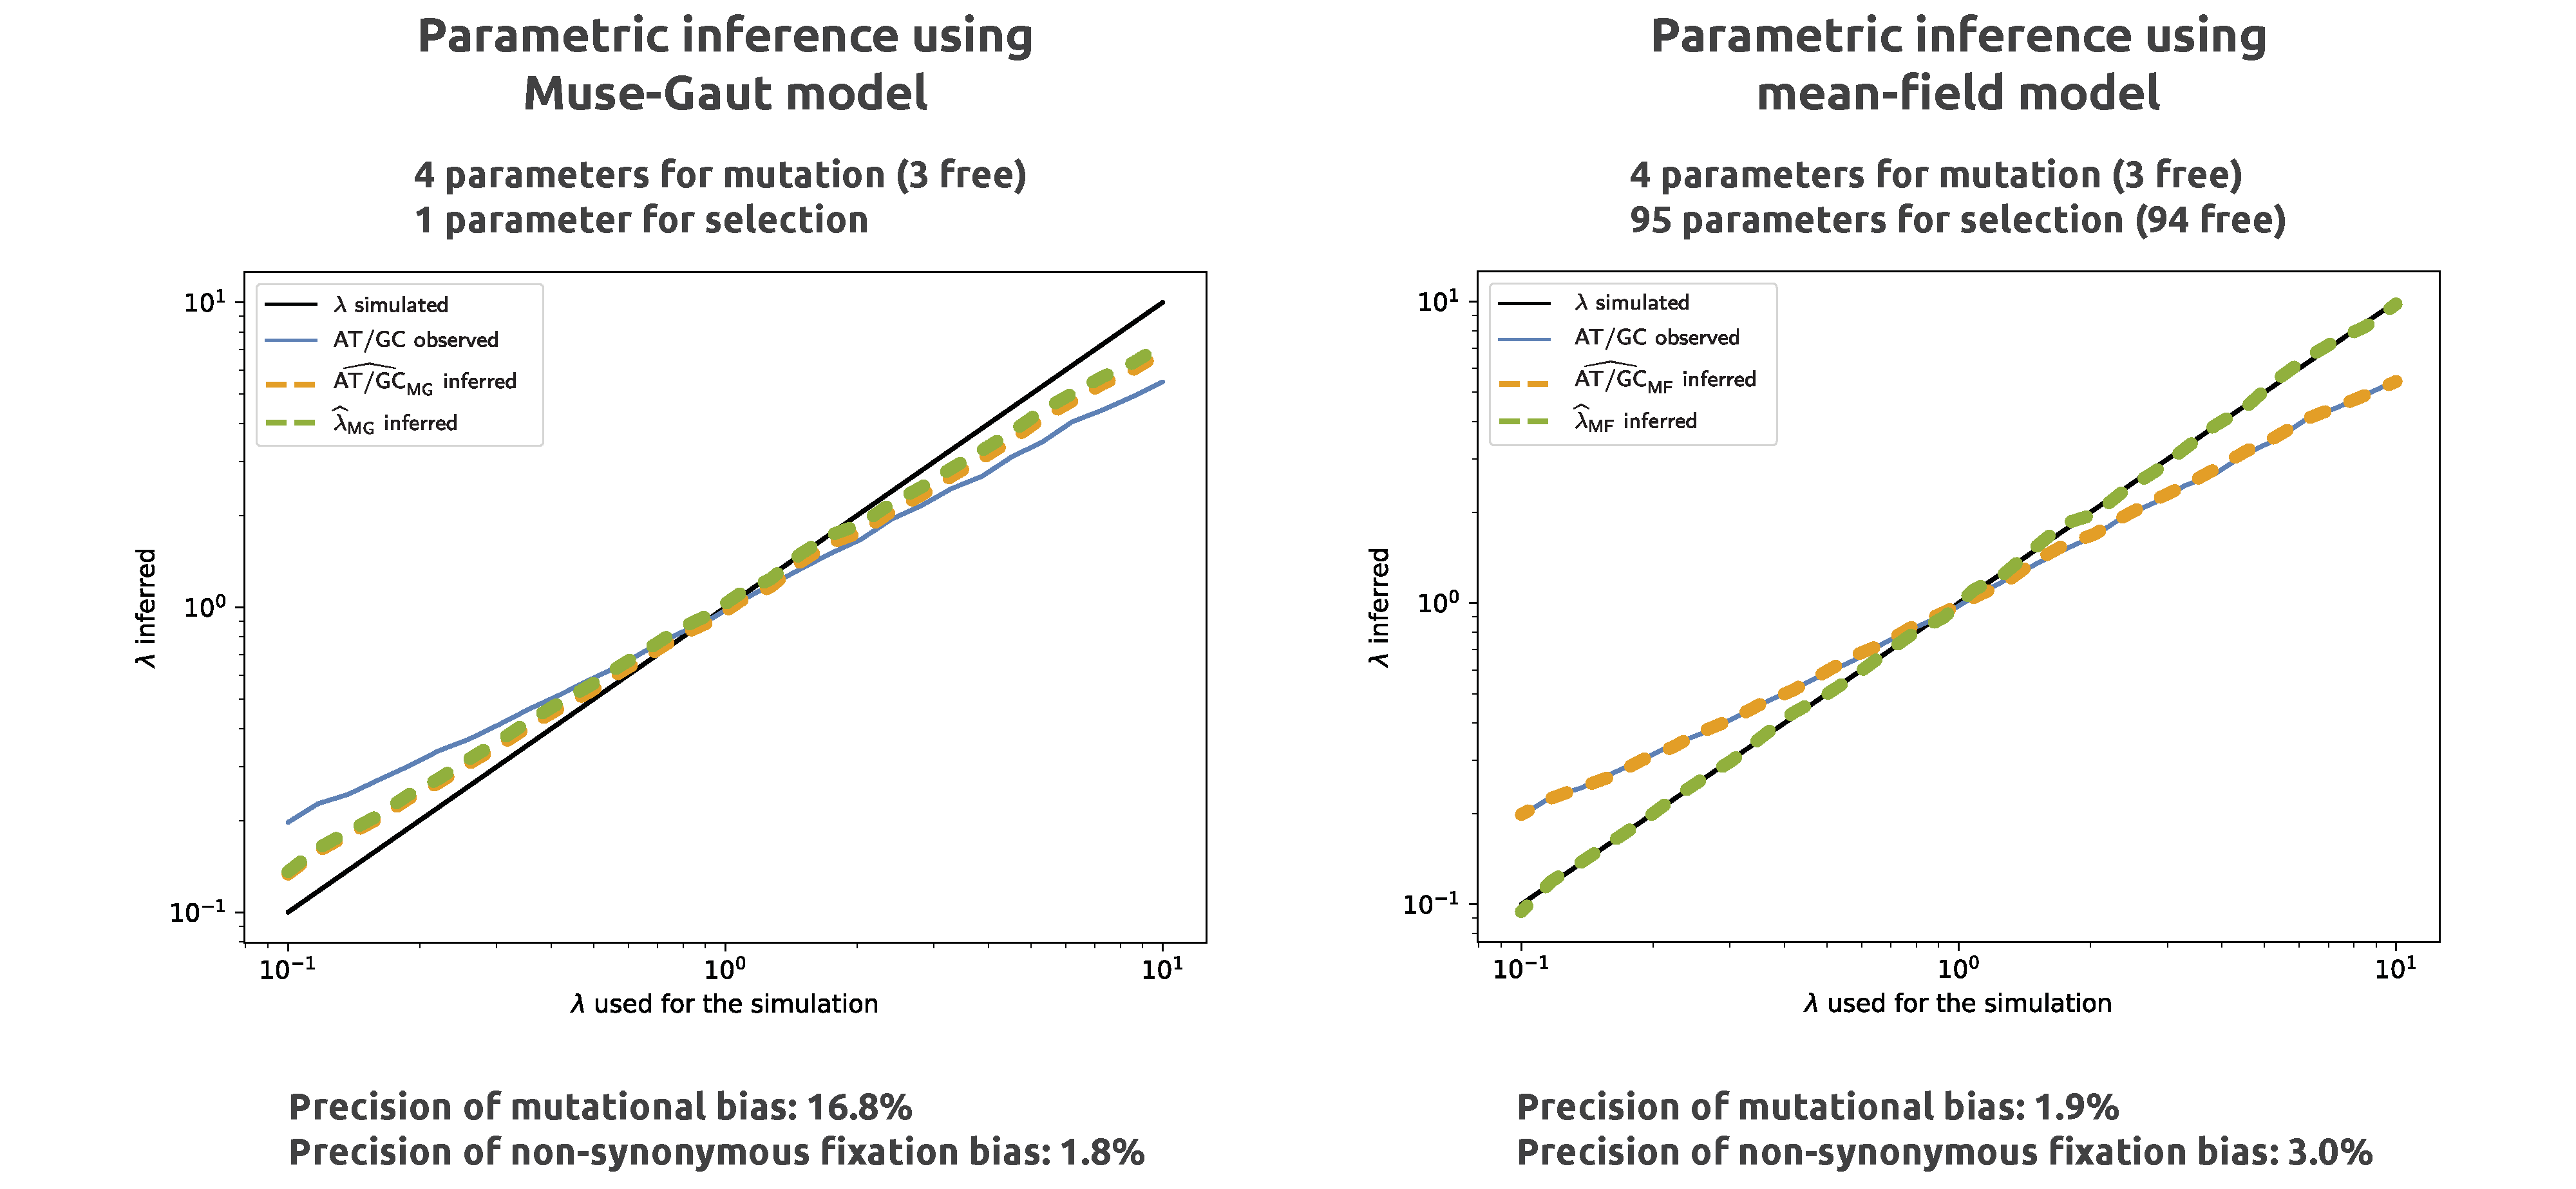
\includegraphics[width=\textwidth] {figures/mut-bias-Simulation-vs-Inference}
	\end{center}
	\caption[Estimation of mutation and fixation bias]{Estimation of mutation and fixation bias. Modeling a single fixation bias leads to skewed estimation of mutation bias. Modeling multiple fixation bias leads to precise estimation of mutation bias. Estimation of fixation bias doesn't depend on the underlying mutation bias.}
\end{figure}

\subsection{Experiment I: Nucleoprotein}
Alignment of 498 amino-acids available for 180 species.
\begin{itemize}
	\item AT/GC of the alignment is 1.15.
	\item Mutational bias $\left({\widehat{\lambda}_{\text{MG}}} \right)$ inferred using Muse-Gaut model is 1.39.
	\item Mutational bias $\left({\widehat{\lambda}_{\text{MF}}} \right)$ inferred using Mean-field model is 1.64.
	\item Fixation bias from AT to GC $\left(\widehat{\omega}_{\textbf{AT} \rightarrow \textbf{GC}}\right)$ inferred using Mean-field model is 0.14.
	\item Fixation bias from GC to AT $\left(\widehat{\omega}_{\textbf{GC} \rightarrow \textbf{AT}}\right)$ inferred using Mean-field model is 0.10.
\end{itemize}
\subsection{Experiment II: Lactamase}
Alignment of 263 amino-acids available for 85 species.
\begin{itemize}
	\item AT/GC of the alignment is 0.79.
	\item Mutational bias $\left({\widehat{\lambda}_{\text{MG}}} \right)$ inferred using Muse-Gaut model is 0.85.
	\item Mutational bias $\left({\widehat{\lambda}_{\text{MF}}} \right)$ inferred using Mean-field model is 0.68.
	\item Fixation bias from AT to GC $\left(\widehat{\omega}_{\textbf{AT} \rightarrow \textbf{GC}}\right)$ inferred using Mean-field model is 0.31.
	\item Fixation bias from GC to AT $\left(\widehat{\omega}_{\textbf{GC} \rightarrow \textbf{AT}}\right)$ inferred using Mean-field model is 0.44.
\end{itemize}

The observed composition of the alignment is the result of the articulation between mutation and selection.
Mutational bias is balanced by a fixation bias (selection) in the opposite direction, potentially a confounding effect with gBGC.
Inference of mutational bias requires to model fixation bias in different direction.
Our mean-field parametric framework is not site-wise, but can be used to untangle mutation and selection, potentially in the presence of fluctuating selection or epistasis.


\chapter[Inferring long-term population size] {Inferring long-term demographic history with Mutation-Selection models.}
{\hypersetup{linkcolor=GREYDARK}\minitoc}


\section{Introduction}
\label{sec:Introduction}
In phylogenetic reconstruction, evolution is generally seen as a stochastic process, whereby point mutations at the level of individuals are subject to evolutionary forces such as selection and random drift, leading to \glspl{substitution} at the level of the population.
Under this framework, the past-history of \glspl{substitution} can be inferred from present-day populations, since each population have been shaped by a particular past-history evolutionary scenario.
As a result, present-day molecular \acrshort{DNA} sequences inform us theoretically on long-term trends in mutation, selection and random drift.
Independently, ecological properties such as phenotypic characters or life-history traits can be observed on extinct or present-day species, and reconstructed for the unobserved ancestral species.
Together, evolutionary and ecological mechanisms can be unraveled by comparing past-history of ecological traits and their correlation to mutation, selection and random drift.

Practically, in order to disentangle mutation, selection and random drift shaping molecular sequences along the phylogenetic tree, we need to decompose our \glspl{substitution} into different categories, where each category is subject to contrasted strength of mutation, selection and random drift such that we can expect to discriminate the strength of each force.
In protein coding \acrshort{DNA} sequences, we can first assume the mutational process to occur at the \acrshort{DNA} level, whereas selection and random drift processes can be assumed to occur only at the protein level in first approximation.
Assuming \glspl{synonymous} are selectively \gls{neutral} allows us to infer the pattern of mutation, free of selection and random drift.

Non-synonymous \glspl{substitution} change the amino-acid sequence, and by comparing their \glspl{substitution} rate relative to the \gls{synonymous} rate (the ratio $\dnds$), we can estimate the global strength of selection and random drift.
Such method has been leveraged in original \gls{codon} models \citep{Muse1994,Goldman1994} to detect proteins under adaptive selection.
However the detection of adaptive evolution as been proved difficult since both pervasive purifying selection and adaptation are entangled into $\dnds$ \citep{Yang2000}.
Moreover, these phenomenological \gls{codon} models do not explicitly model selection and random drift, meaning the \gls{non-synonymous} rate cannot be explicitly related to selection (purifying or adaptive) and random drift.

Mechanistic \gls{codon} models explicitly introduced population-genetics equations into phylogenetic \gls{codon} models \citep{Halpern1998}.
These so called mutation-selection \gls{codon} models assign a different fitness for each amino-acid at given specific \gls{codon} site of the \acrshort{DNA} sequence.
As such they assume a static fitness landscape of amino-acids along the phylogeny, providing a model of purifying selection where the least fit amino-acids are purified away \citep{Rodrigue2010,Rodrigue2014,Tamuri2012,Tamuri2014}.
Modeling explicitly purifying selection proved to be a valuable null (\gls{nearly-neutral}) model against which to test for the presence of adaptation \citep{Rodrigue2016,Bloom2017}.
These methods have so far assumed the strength of random drift to be constant across the phylogeny.

Drift, which is proportional to the inverse of effective population size~($\Ne$), can not be realistically assumed constant \citep{Ohta1992}.
Estimation of $\Ne$ using polymorphism sequence data obtained from a diverse array of species have demonstrated that the range of $\Ne$ varies by orders of magnitude in mammals \citep{Galtier2016}, in drosophila \citep{Benger2013,Keightley2016}.
Relaxing the assumption of constant random drift in mutation-selection \gls{codon} models is necessary to account for empirically grounded
assumptions.
Practically, can we mathematically model long-term fluctuation of $\Ne$ in mutation-selection model?
Empirically do we have enough signal in alignment data, and computational tools, to estimate fluctuations of $\Ne$?

Independent empirical experiments have sought to correlate life-history traits and population-genetic parameters of evolution under the molecular comparative method \citep{Lartillot2011,Weber2014}.
They have proved that $\dnds$ is correlated to life-history traits, such as body mass and longevity, thought the direction of correlation could not be replicated across all experiments \citep{Figuet2016}.
The expected correlation under the \gls{nearly-neutral} theory of evolution is that population with low $\Ne$ would have both a large body size and a high $\dnds$ due to the increase of random drift.
However, the relationship between $\Ne$ and $\dnds$ is far for from being linear nor $1$-to-$1$, due to contrasted effect of selection merged into a single phenomenological parameter and due to non-equilibrium properties \citep{Jones2016}.
The mutation-selection models now give us leverage to revisit these studies by incorporating explicitly $\Ne$ as a parameter of the model.
With this in mind, can we craft a framework which could allow us to correlate ecological life-history traits (longevity, maturity, weight, size, \ldots) to effective population size~($\Ne$) and mutation rate per unit of time~($\mu$)?

Here we introduce a model of site-heterogeneous selection, and branch-heterogeneous traits~($\mu$, $\Ne$ and life-history traits).
Our model can be seen as the integration between the mutation-selection framework estimating site-heterogeneous selection coefficients \citep{Rodrigue2014,Tamuri2014}, and the molecular comparative framework modeling the joint evolution of life-history and molecular traits \citep{Lartillot2011,Weber2014}.
We test our model and inference framework against simulated data made under more realistic assumptions, and with empirical data while correlating life-history traits and population-genetic parameters of evolution.
Broadly, these framework aims to shade light on the long-term ecological and evolutionary process shaping the history of molecular sequences.

\section{New approaches}
\label{sec:NewApproaches}
\begin{figure}[H]
	\centering
	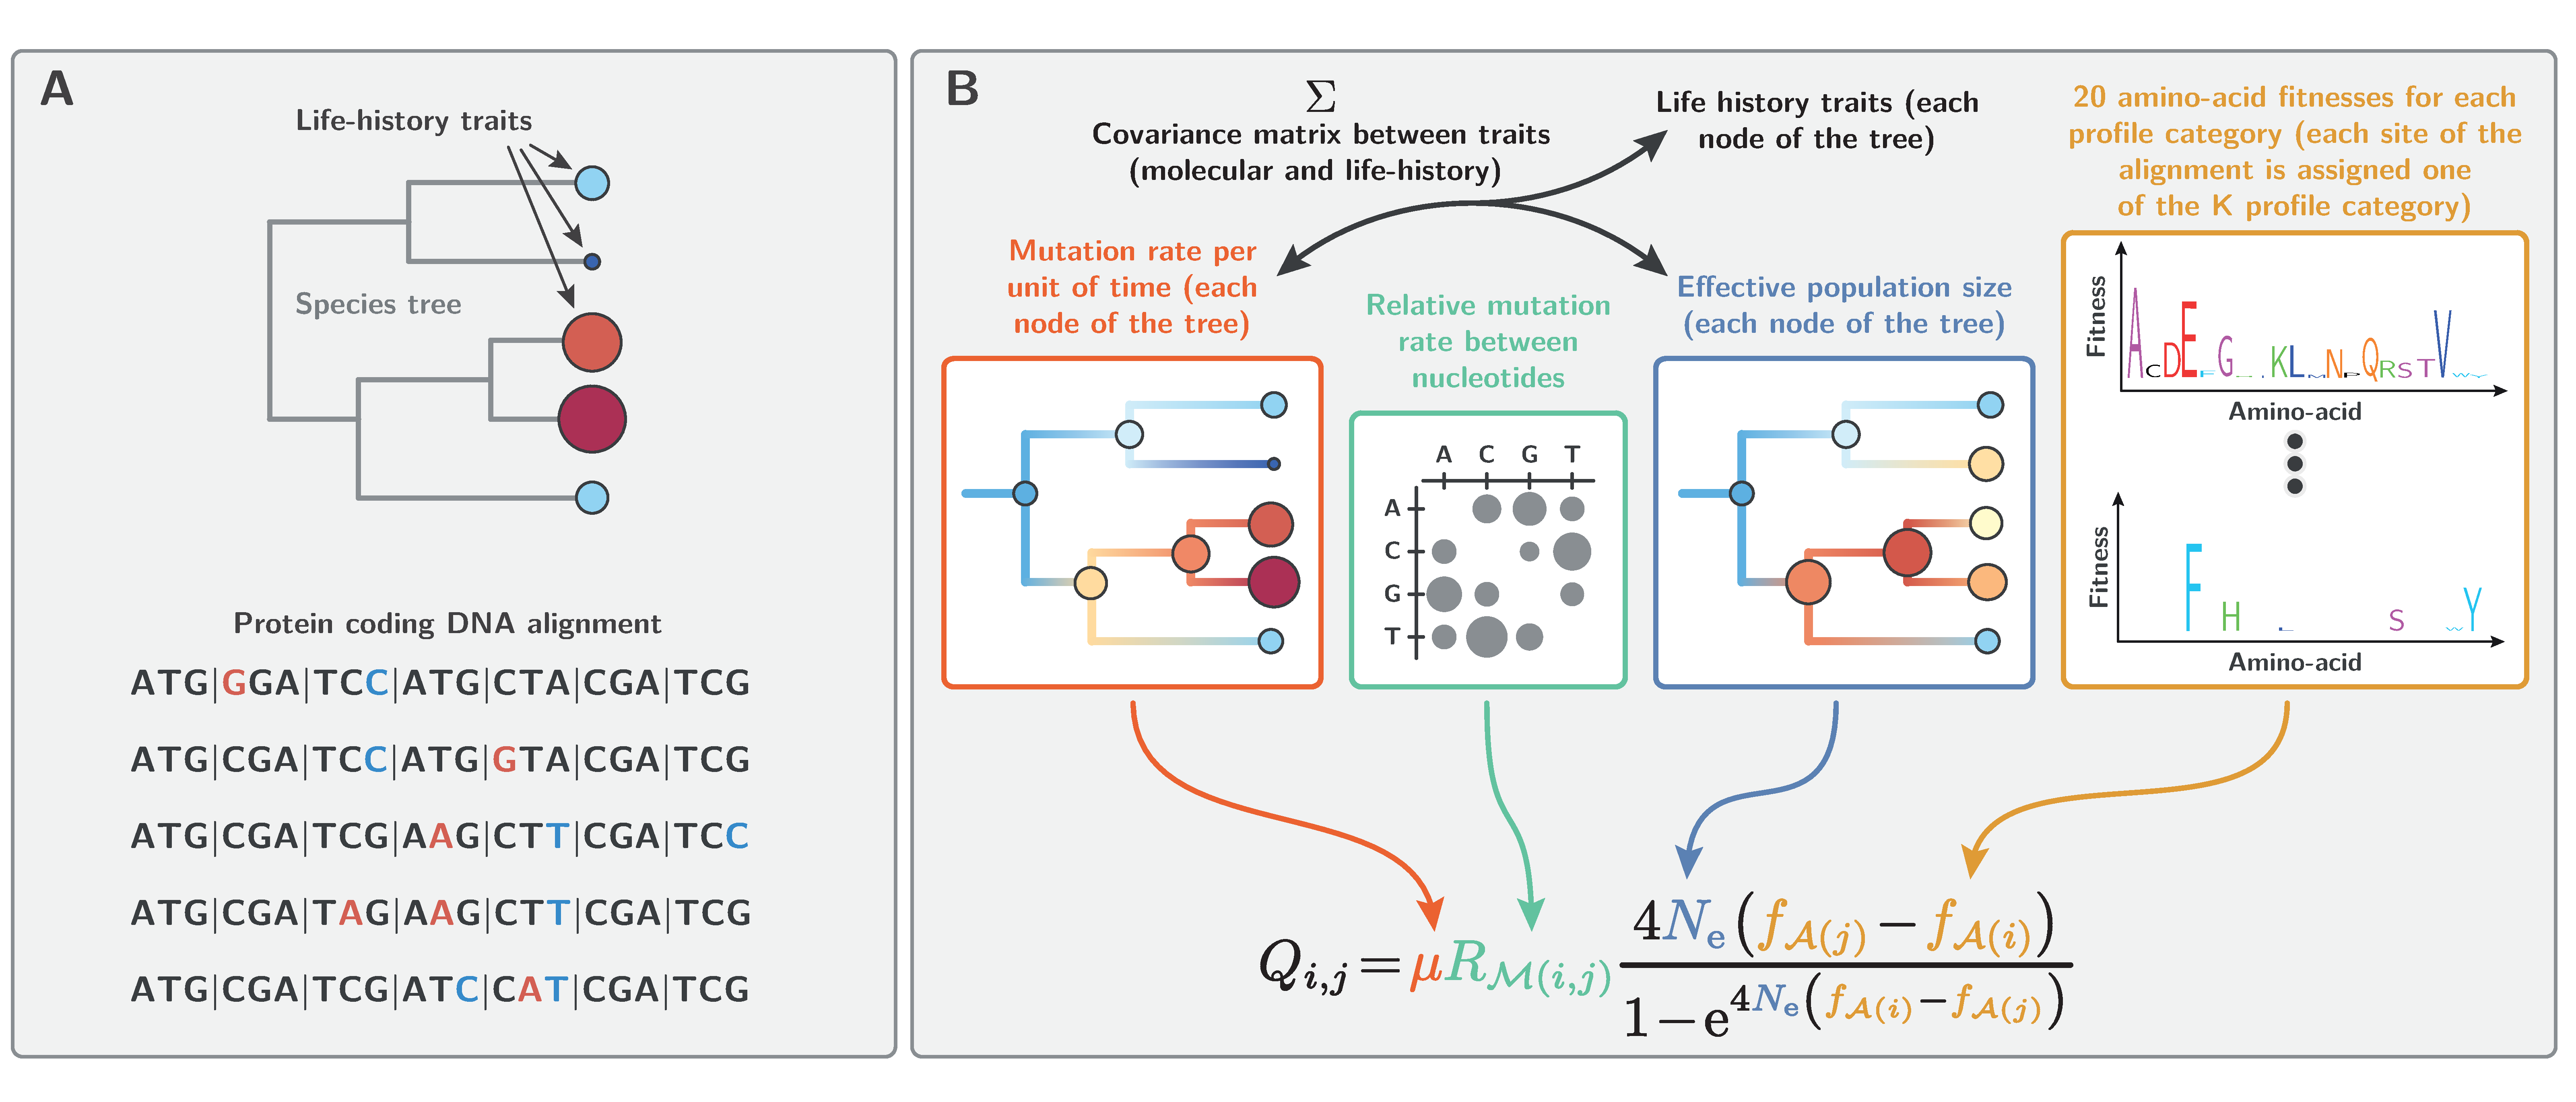
\includegraphics[width=\textwidth] {model_summary.pdf}
	\caption[Model summary]{
		Model summary.
		Panel A.
		Our method requires a given rooted topology, and an alignment of protein coding \acrshort{DNA} for the extant species.
		Optionally, the method can use quantitative life-history traits at the leaves of the tree, and dated estimation for the internal nodes of the tree.
		Panel B.
		Our Bayesian inference model estimates selection coefficients, mutation rate, intensity of random drift and the age of the internal nodes.
		Effective population since~($\Ne$) and mutation rate per unit of time~($\mu$) are considered fluctuating branch-wise, but assumed constant across all sites of the \acrshort{DNA} sequence.
		Conversely, the selection coefficient of amino-acids are considered changing for sites along the \acrshort{DNA} sequence, but are considered constant across the tree.
		Branch-heterogeneity is modeled as an auto-correlated log-Brownian process, meaning our model estimates correlation coefficients between quantitative traits (as input), $\Ne$, and $\mu$, where phylogenetic inertia is accounted for.
		Synonymous \glspl{substitution} are leveraged to estimates branch-wise mutation rate~($\mu$).
		Site-specific rates of \glspl{non-synonymous} across the tree is leveraged to estimate site-wise selection coefficient~($\Fit$).
		Branch-specific rates of \glspl{non-synonymous} across the sequence is leveraged to estimate branch-wise random drift~($\Ne$).
	}
	\label{fig:modelSummary}
\end{figure}

\subsection{Substitution rate equation}
\label{sec:MutSelEq}
DNA coding sequences are modeled at the level of the \gls{codon}, where for each site (counted by triplets in the alignment), a change of \gls{codon} means a change in \acrshort{DNA} but not necessarily in amino-acid.
The \gls{substitution} rate (per unit of time) from \gls{codon} $\ci$ to $\cj$, denoted $\submatrix_{\itoj}$, is equal to the total rate of mutation (per unit of time) at the level of the population~($2\Ne\mu_{\itoj}$) multiplied by the probability of fixation of the mutation:
\begin{equation}
{\submatrix_{\itoj}} = 2 \Ne \mu_{\itoj} p_{\mathrm{fix}}(\itoj)
\end{equation}

In the case of synonymous mutations, which we assumed are \gls{neutral}, the probability of fixation is independent of the original and target \gls{codon}, and equal $1/2 \Ne$.
Finally ${\submatrix_{\itoj}}$ simplifies to: 
\begin{equation}
\submatrix_{\itoj} = \mu_{\itoj}
\end{equation}

In the case of non-synonymous mutations, the probability of fixation depends on the difference in fitness between the amino-acid encoded by the initial and final \glspl{codon} \citep{Ohta1992}:
\begin{equation}
\label{eq:mutationSelection}
{\submatrix_{\itoj}} = \mu_{\itoj} \dfrac{4 \Ne \left({\fitj - \fiti}\right)}{{1 - \e^{4 \Ne \left({\fiti - \fitj}\right)} }}
\end{equation}
where $\Fit$ is a $20$-dimensional vector specifying the log-fitness for each amino-acid, and $\aai$ is the amino-acid encoded by \gls{codon} $i$.
We see from this equation that, $\fit$ and $\Ne$ are confounded, such that increasing the \gls{effective-population-size} while decreasing the fitnesses by the same factor leads to the same \gls{substitution} rate.

The mutation rate $\mu_{\itoj}$ depends on the underlying nucleotide change between the \glspl{codon} $\ci$ and $\cj$.
First, if \gls{codon} $\ci$ to $\cj$ are not neighbors, $\mu_{\itoj}$ is equal to $0$.

Second, if \gls{codon} $\ci$ and $\cj$ are only one mutation away, $\mu_{\itoj}$ is given by the nucleotide relative rate~(${\mutmatrix_{\nucitoj}}$) scaled by the mutation rate per time~($\mu$).
Technically, the $4$-dimensional nucleotide relative rate matrix~($\Mutmatrix$) is normalized such that we expect $1$ \gls{substitution} per unit of time, hence the scaling by $\mu$.

\subsection{Site-selection model}
\label{sec:SiteHetero}
The strength of selection is not typically homogeneous along the sequence.
For example, exposed sites are under lower selective pressure than buried sites \citep{Echave2016}.
In fact, selection differs in a way that depends on the local physico-chemical requirements \citep{Goldstein2016,Goldstein2017,Weber2019}.
Following the seminal work on mutation-selection models \citep{Halpern1998}, one increasingly popular way to account for this variation is to allow for site-specific amino-acid fitness profiles (20-dimensional vectors).

The sparcity of signal per site requires to aggregate sites together in categories, such as to fit the amino-acid fitnesses.
Conversely, the category assigned to each site is fitted such that the sites aggregated into the same category share the pattern of selection and hopefully the same physico-chemical properties.
The methods previously developed to estimate site-heterogeneous amino-acid fitnesses relied on penalized-likelihood \citep{Tamuri2012,Tamuri2014}, or a Bayesian non-parametric random-effect approach \citep{Rodrigue2010,Rodrigue2014,Rodrigue2016}.
The work presented here relies on the Bayesian approach, as in \textit{PhyloBayes} \citep{Rodrigue2010}.

\subsection{Branch-traits model}
\label{sec:BranchHetero}
Many phenotypic traits can vary between species, either evolutionary parameters of interest, environmental variables or life-history traits \citep{Felsenstein1985,Romiguier2014}.
However, the value of a trait along a branch is expected to be dependent on the value at the parent branch, such that abrupt shifts on trait value should be penalized \citep{Huelsenbeck2003,Seo2004}.
Moreover, some of these traits might be correlated, for example an increase in $\Ne$ might be correlated with a decrease in body size \citep{Weber2014,Romiguier2014}.

Correlation of traits has previously been modeled using diffusive log-Brownian multivariate process along a phylogeny \citep{Seo2004,Lartillot2011}.
Under a log-Brownian process, the logarithm of the trait value at a given node of the tree is normally distributed, with mean equal to the log-value at parent node, and the standard deviation is proportional to the branch size (in unit of time).

In a multivariate process, traits are modeled together as a vector-valued time-dependent random process, parameterized by a covariance matrix between traits~($\Covariancematrix$).
Altogether, values of the multivariate process at each node of the tree, a covariance matrix and divergence times are jointly estimated.
Once the traits are sampled at all nodes, traits along each branch is taken as the average (see Methods) between extremities of this branch.
The work presented here implemented the branch-heterogeneity in a Bayesian context, as in \textit{CoEvol} \citep{Lartillot2011}.
Technically, the precision matrix (invert of covariance matrix) is distributed as an invert Wishart, meaning the \gls{prior} matrix is diagonal pushing the correlation coefficients toward $0$.

\subsection{Mutation-selection-random drift model}
\label{sec:BranchSiteHetero}
Our Bayesian inference model (see Methods) can be viewed as an integration between mutation-selection models accounting for site-heterogeneity of selection coefficients, and the molecular comparative approach accounting for variation in molecular and phenotypic or life-history traits between species.
More specifically, in the model now presented, $\Ne$ and $\mu$ are allowed to vary between species (across branches), but assumed constant along the \acrshort{DNA} sequence.
Conversely, amino-acid fitness profiles are assumed to vary across sites, but are considered constant along the tree (Figure~\ref{fig:modelSummary}).

The phylogenetic \gls{codon} model presented here makes several additional assumptions on the evolutionary processes generating the observed alignment.
First, the species tree topology is supposed to be known, and each gene should match the species tree, meaning genes are strict orthologs (no paralogs and no horizontal transfers).
Second, there is no epistasis (interaction between sites), such that any position of the sequence has its own independent evolutionary process and a \gls{substitution} at one position does not affect the \gls{substitution} process at other positions.
Third, from a population genetic perspective, we assumed sites of the protein to be unlinked, or equivalently the mutation rate is low enough such that there is no Hill-Robertson interference nor genetic hitch-hiking.
Fourth, we assume \acrshort{DNA} sequences to be representative of the species, not taking into account the sampling effect tending to over-represent weakly deleterious mutations present at low frequencies.


Our Bayesian implementation, written in C++ is publicly available at \url{https://github.com/bayesiancook/bayescode/tree/chronogram}.

\begin{figure}[htb]
	\centering
	\begin{minipage}{0.32\linewidth}
		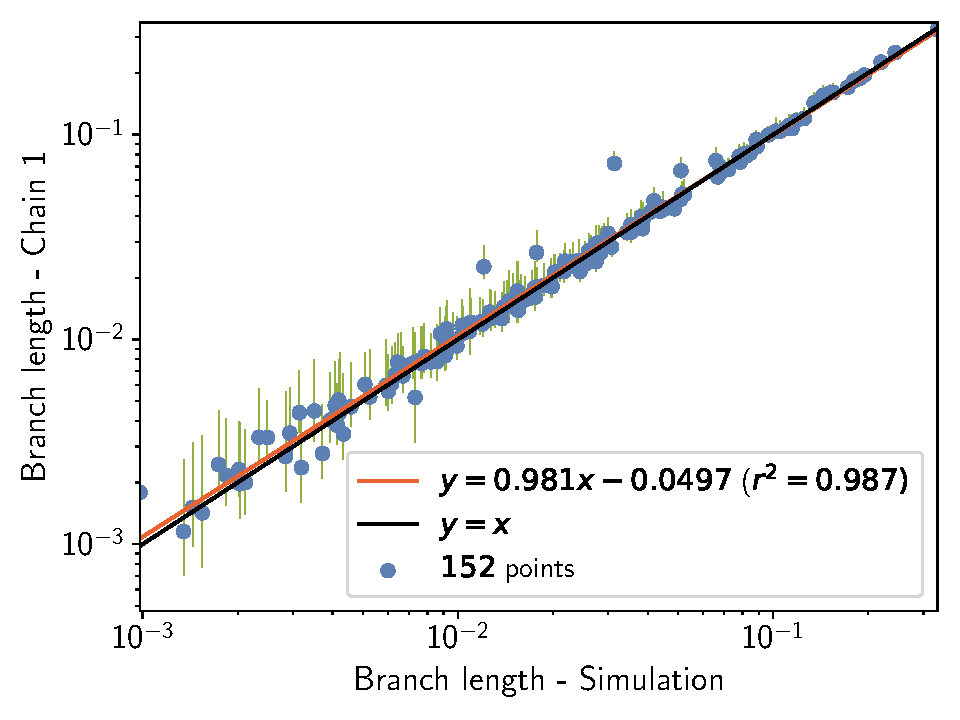
\includegraphics[width=\linewidth, page=1]{simulations/BranchWise_SimuDiv_SiteMutSelBranchNe_BranchCorrelation_Log10BranchLength}
	\end{minipage}	\hfill
	\begin{minipage}{0.32\linewidth}
		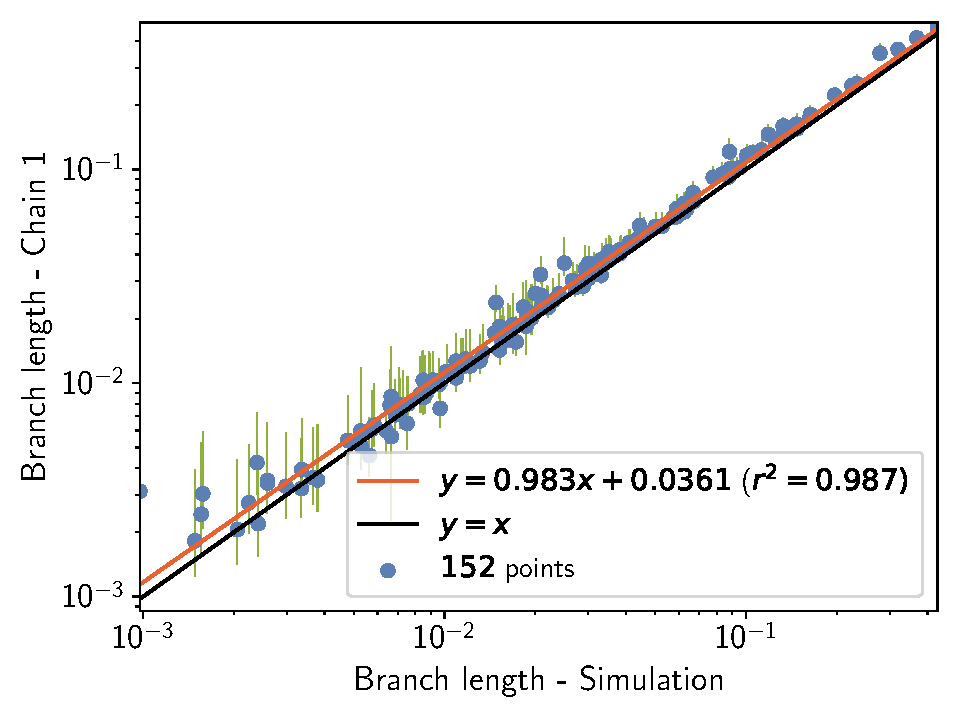
\includegraphics[width=\linewidth, page=1]{simulations/SimuPoly_SiteMutSelBranchNe_BranchCorrelation_Log10BranchLength}
	\end{minipage}	\hfill
	\begin{minipage}{0.32\linewidth}
		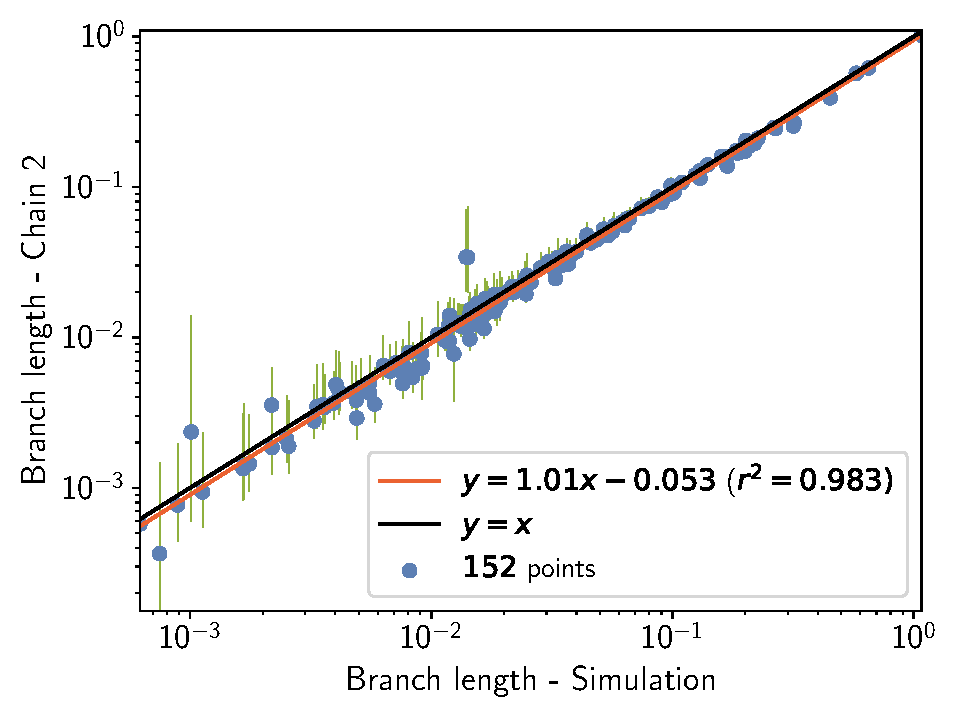
\includegraphics[width=\linewidth, page=1]{simulations/SimuGeo_SiteMutSelBranchNe_BranchCorrelation_Log10BranchLength}
	\end{minipage}	\hfill
	\begin{minipage}{0.32\linewidth}
		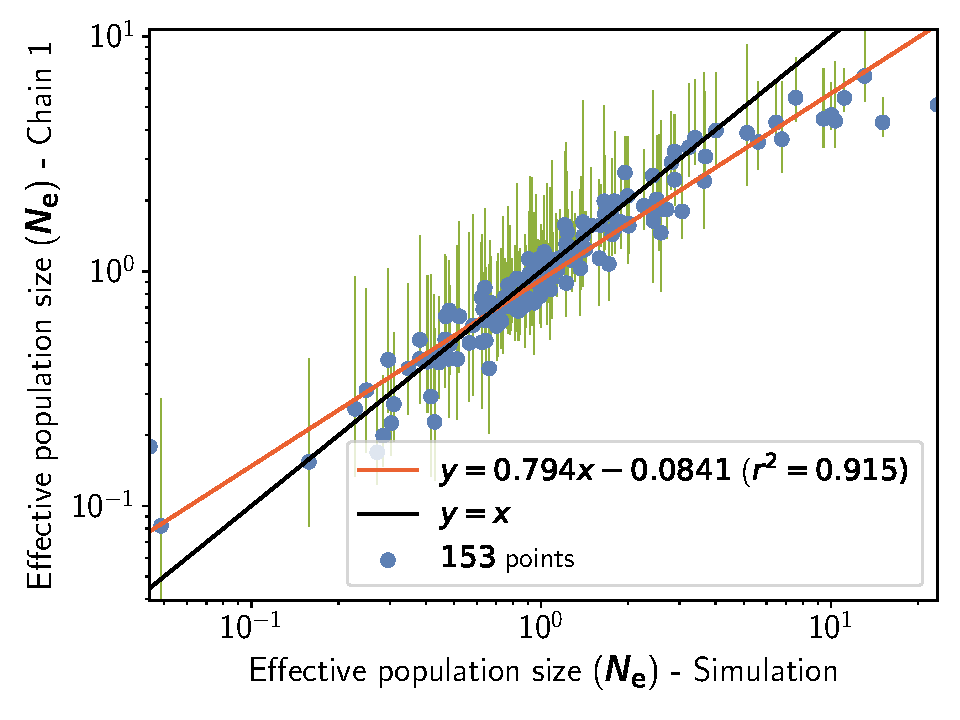
\includegraphics[width=\linewidth, page=1]{simulations/BranchWise_SimuDiv_SiteMutSelBranchNe_BranchCorrelation_LogPopulationSize}
	\end{minipage}	\hfill
	\begin{minipage}{0.32\linewidth}
		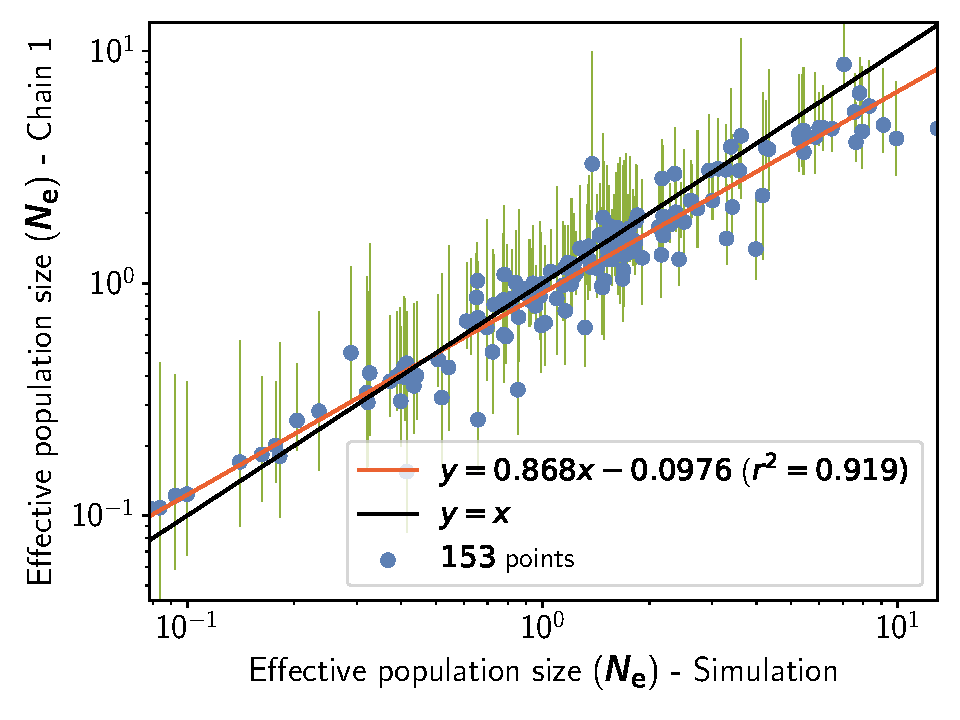
\includegraphics[width=\linewidth, page=1]{simulations/SimuPoly_SiteMutSelBranchNe_BranchCorrelation_LogPopulationSize}
	\end{minipage}	\hfill
	\begin{minipage}{0.32\linewidth}
		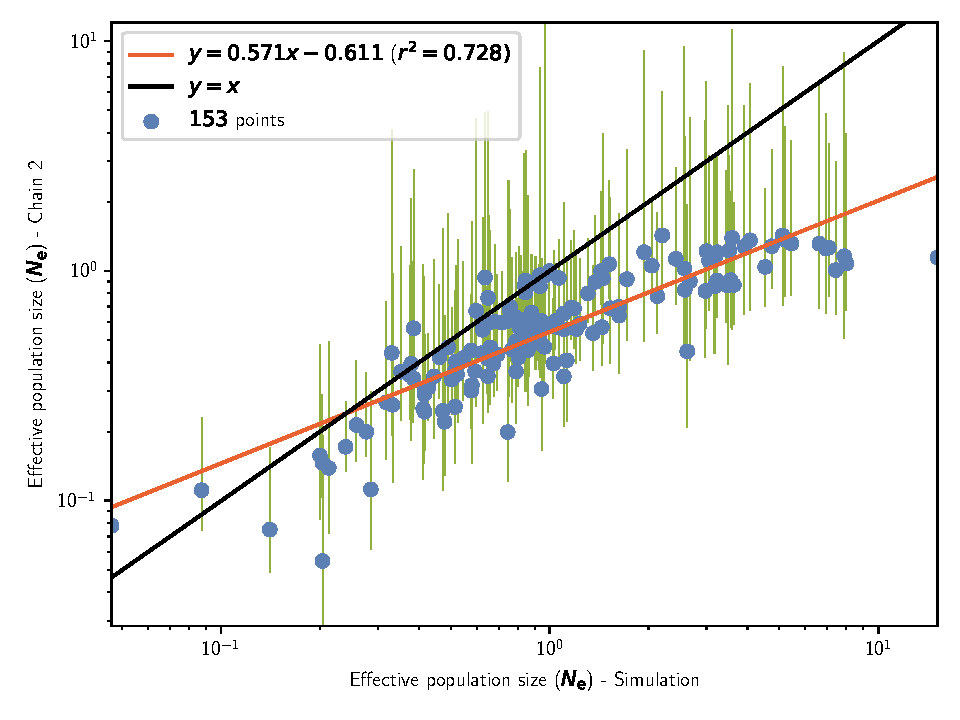
\includegraphics[width=\linewidth, page=1]{simulations/SimuGeo_SiteMutSelBranchNe_BranchCorrelation_LogPopulationSize}
	\end{minipage}	\hfill
	\caption[Inferred and simulated $\Ne$]{
		Inferred and simulated $\Ne$
		Top row, branch length in expected number of \glspl{substitution}, for each branch of the tree.
		Bottom row, $\Ne$ for each node (including leaves) of the tree, relative to $\Ne$ at the root of the tree.
		Left panel, simulation under the mutation-selection approximation, as to test the soundness of the inference framework.
		Middle panel, simulation accounting for small population size effects~($5000$ individuals at the root), site linkage and short term fluctuation of $\Ne$.
		Right panel, simulation accounting for site epistasis, with fluctuation of the selection coefficient along the phylogeny.
		The tree root is $150$ million years old, where the initial population start with a mutation rate of $\smash{1e^{-8}}$ per site per generation, and generation time of $10$ years.
		These experiments confirm that signal in the placental mammalian tree can allow to reliably infer the direction of change in $\Ne$, even if linkage disequilibrium, short term fluctuation of $\Ne$ and finite population size effects are not accounted for in the inference framework.
		However, the presence of epistasis between sites is a serious threat to the inference of $\Ne$.
	}
	\label{fig:simulations}
\end{figure}

\section{Results}
\label{sec:Results}

\subsection{Simulated experiments}
\label{sec:ResultsSimulated}
The inference framework was first tested using independently simulated alignments (see Methods).
With the aim of applying the inference method to empirical dataset in placental mammals and in primates, the simulation parameters were chosen to match the empirical regime of total branch length (expected number of substitutions) from root to leaves.

A first serie of simulations was meant to test the soundness of our inference framework, by simulating essentially under the model used for inference.
The mutation-selection approximation was assumed to be valid, and sites were simulated under different fitness profiles.
In addition, $\Ne$ varies at the tree nodes but otherwise remains constant along each branch.
In this context, simulated branch length and $\Ne$ could be recovered appropriately by our inference method (Figure~\ref{fig:simulations}, panel A \& B).
Unfortunately, assumptions made for this simulations are almost certainly violated in practice.
First, $\Ne$ should change continuously along a branch, between each generation of the population.
Second, having a separate process for each site is equivalent to have no linkage between sites (free recombination), an assumption that should be relaxed. 
Third, the probability of fixation (equation \ref{eq:mutationSelection}) does not hold in small finite population.

For these reasons, we performed a second more challenging series of simulations.
The finite population was modeled explicitly in a Wright-Fisher simulator, tracking the frequency of each \gls{allele} at each generation along the phylogeny.
Such simulator accounts for small population size effects, hitchhiking of weakly deleterious mutations during selective sweep and background selection due to linkage desequilibrium.
Fluctuations of $\Ne$ and mutation rate were also fluctuating continuously along the branch of the tree.
Moreover, noise was added by accounting for short term fluctuations of $\Ne$ on the order of $20\%$ per generation.
The simulated branch length and $\Ne$ could be robustly recovered by the inference framework in this context (Figure~\ref{fig:simulations}, panel C \& D).

However, if the results are encouraging to apply the method on empirical data, we rely on the assumption of site-independent fitness landscape, which is almost certainly broken in practice.
Finally, we implemented a more complex, site-dependent fitness landscape accounting for the $3$-dimensional structure of protein and interaction between sites.
In such a model, the folding energy of the protein determines the probability of being in the folded state, a proxy for fitness \citep{Goldstein2017}.
During a simulation, at a particular \gls{codon} site, the fitness landscape is dependent on the actual amino-acids present in the vicinity of this particular site.
Our inference framework could recover the simulated branch length, but had more difficulties to retrieve the simulated $\Ne$ in the context of site-dependent epistasis (Figure~\ref{fig:simulations}, panel E \& F)

\subsection{Empirical experiments}
\label{sec:ResultsEmpirical}
\begin{figure}[H]
	\centering
	\begin{minipage}{0.411\linewidth}
		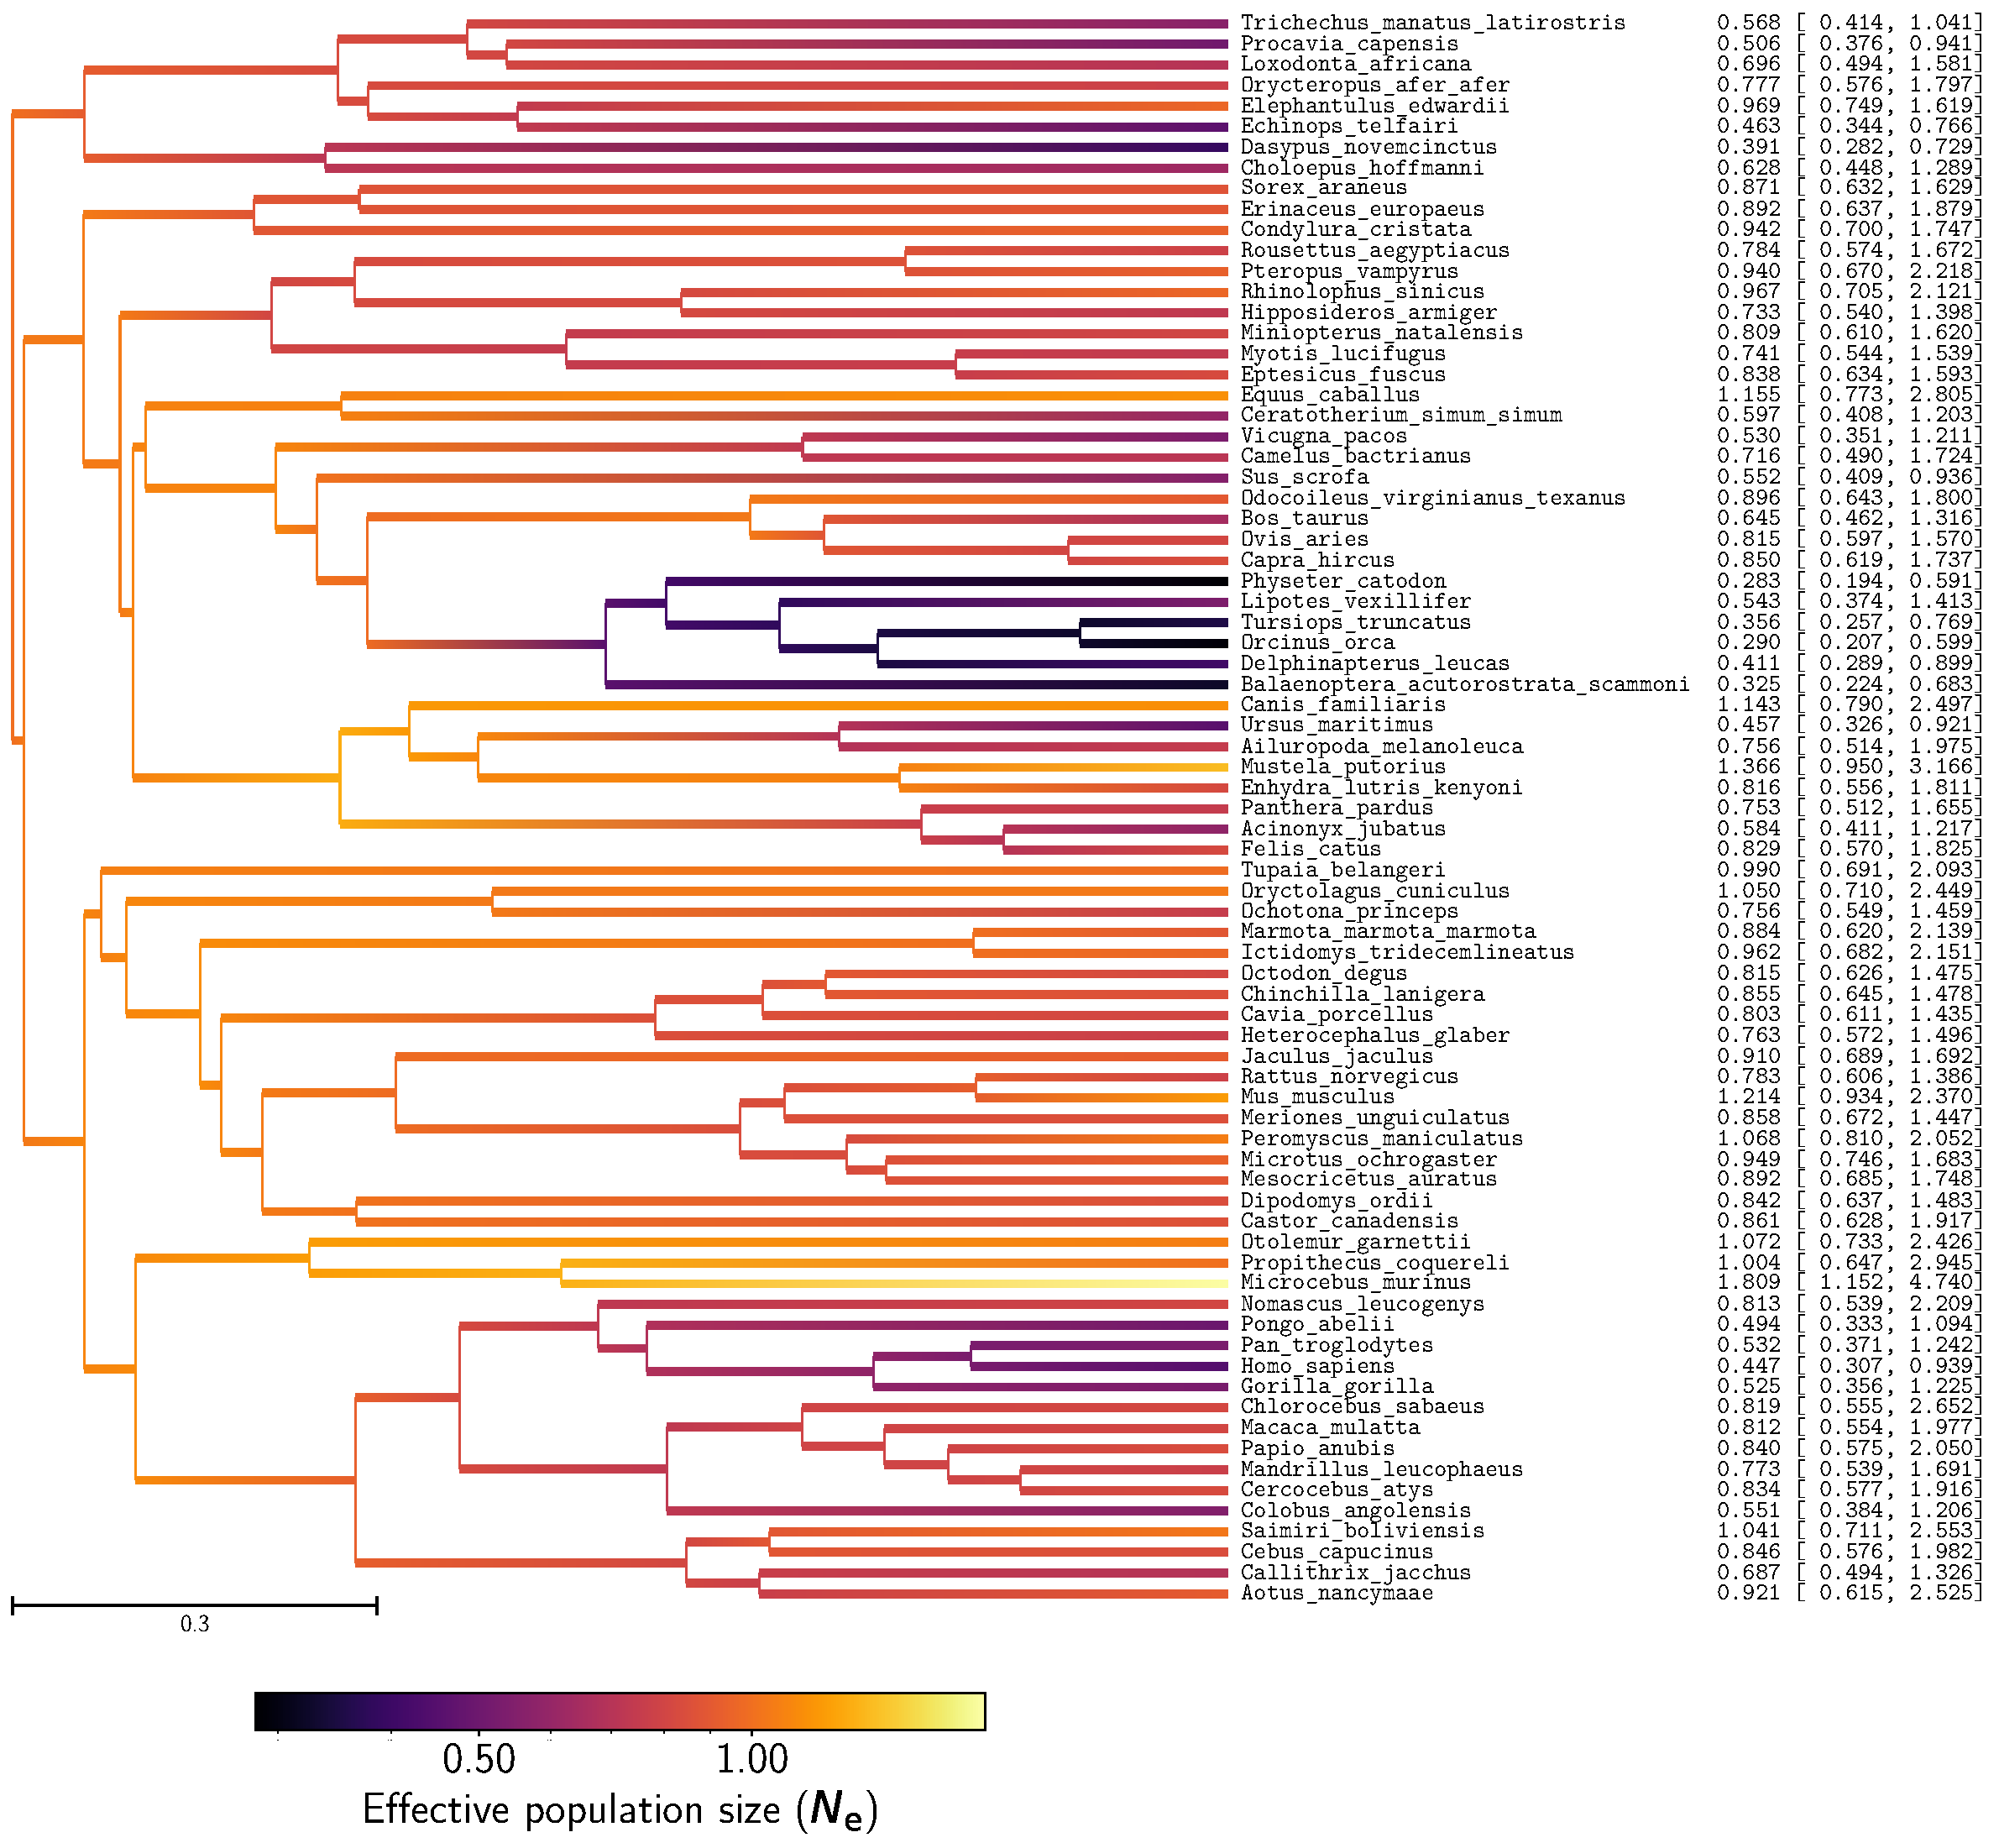
\includegraphics[valign=t, width=\linewidth, page=1, clip, trim=0cm 0cm 15.35cm 0.15cm]{mammals/18CDS_SiteMutSelBranchNe_R1_LogPopulationSize}
	\end{minipage}
	\begin{minipage}{0.158\linewidth}
		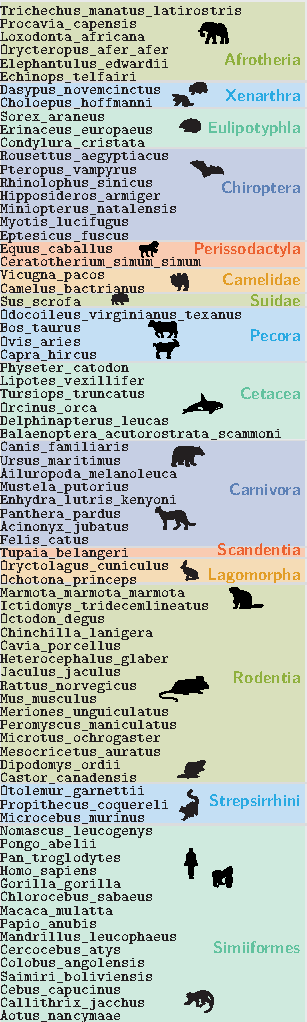
\includegraphics[valign=t, width=\linewidth, page=1, clip, trim=0cm -2.2cm 0cm 0cm]{mammals_species}
	\end{minipage}
	\begin{minipage}{0.411\linewidth}
		\reflectbox{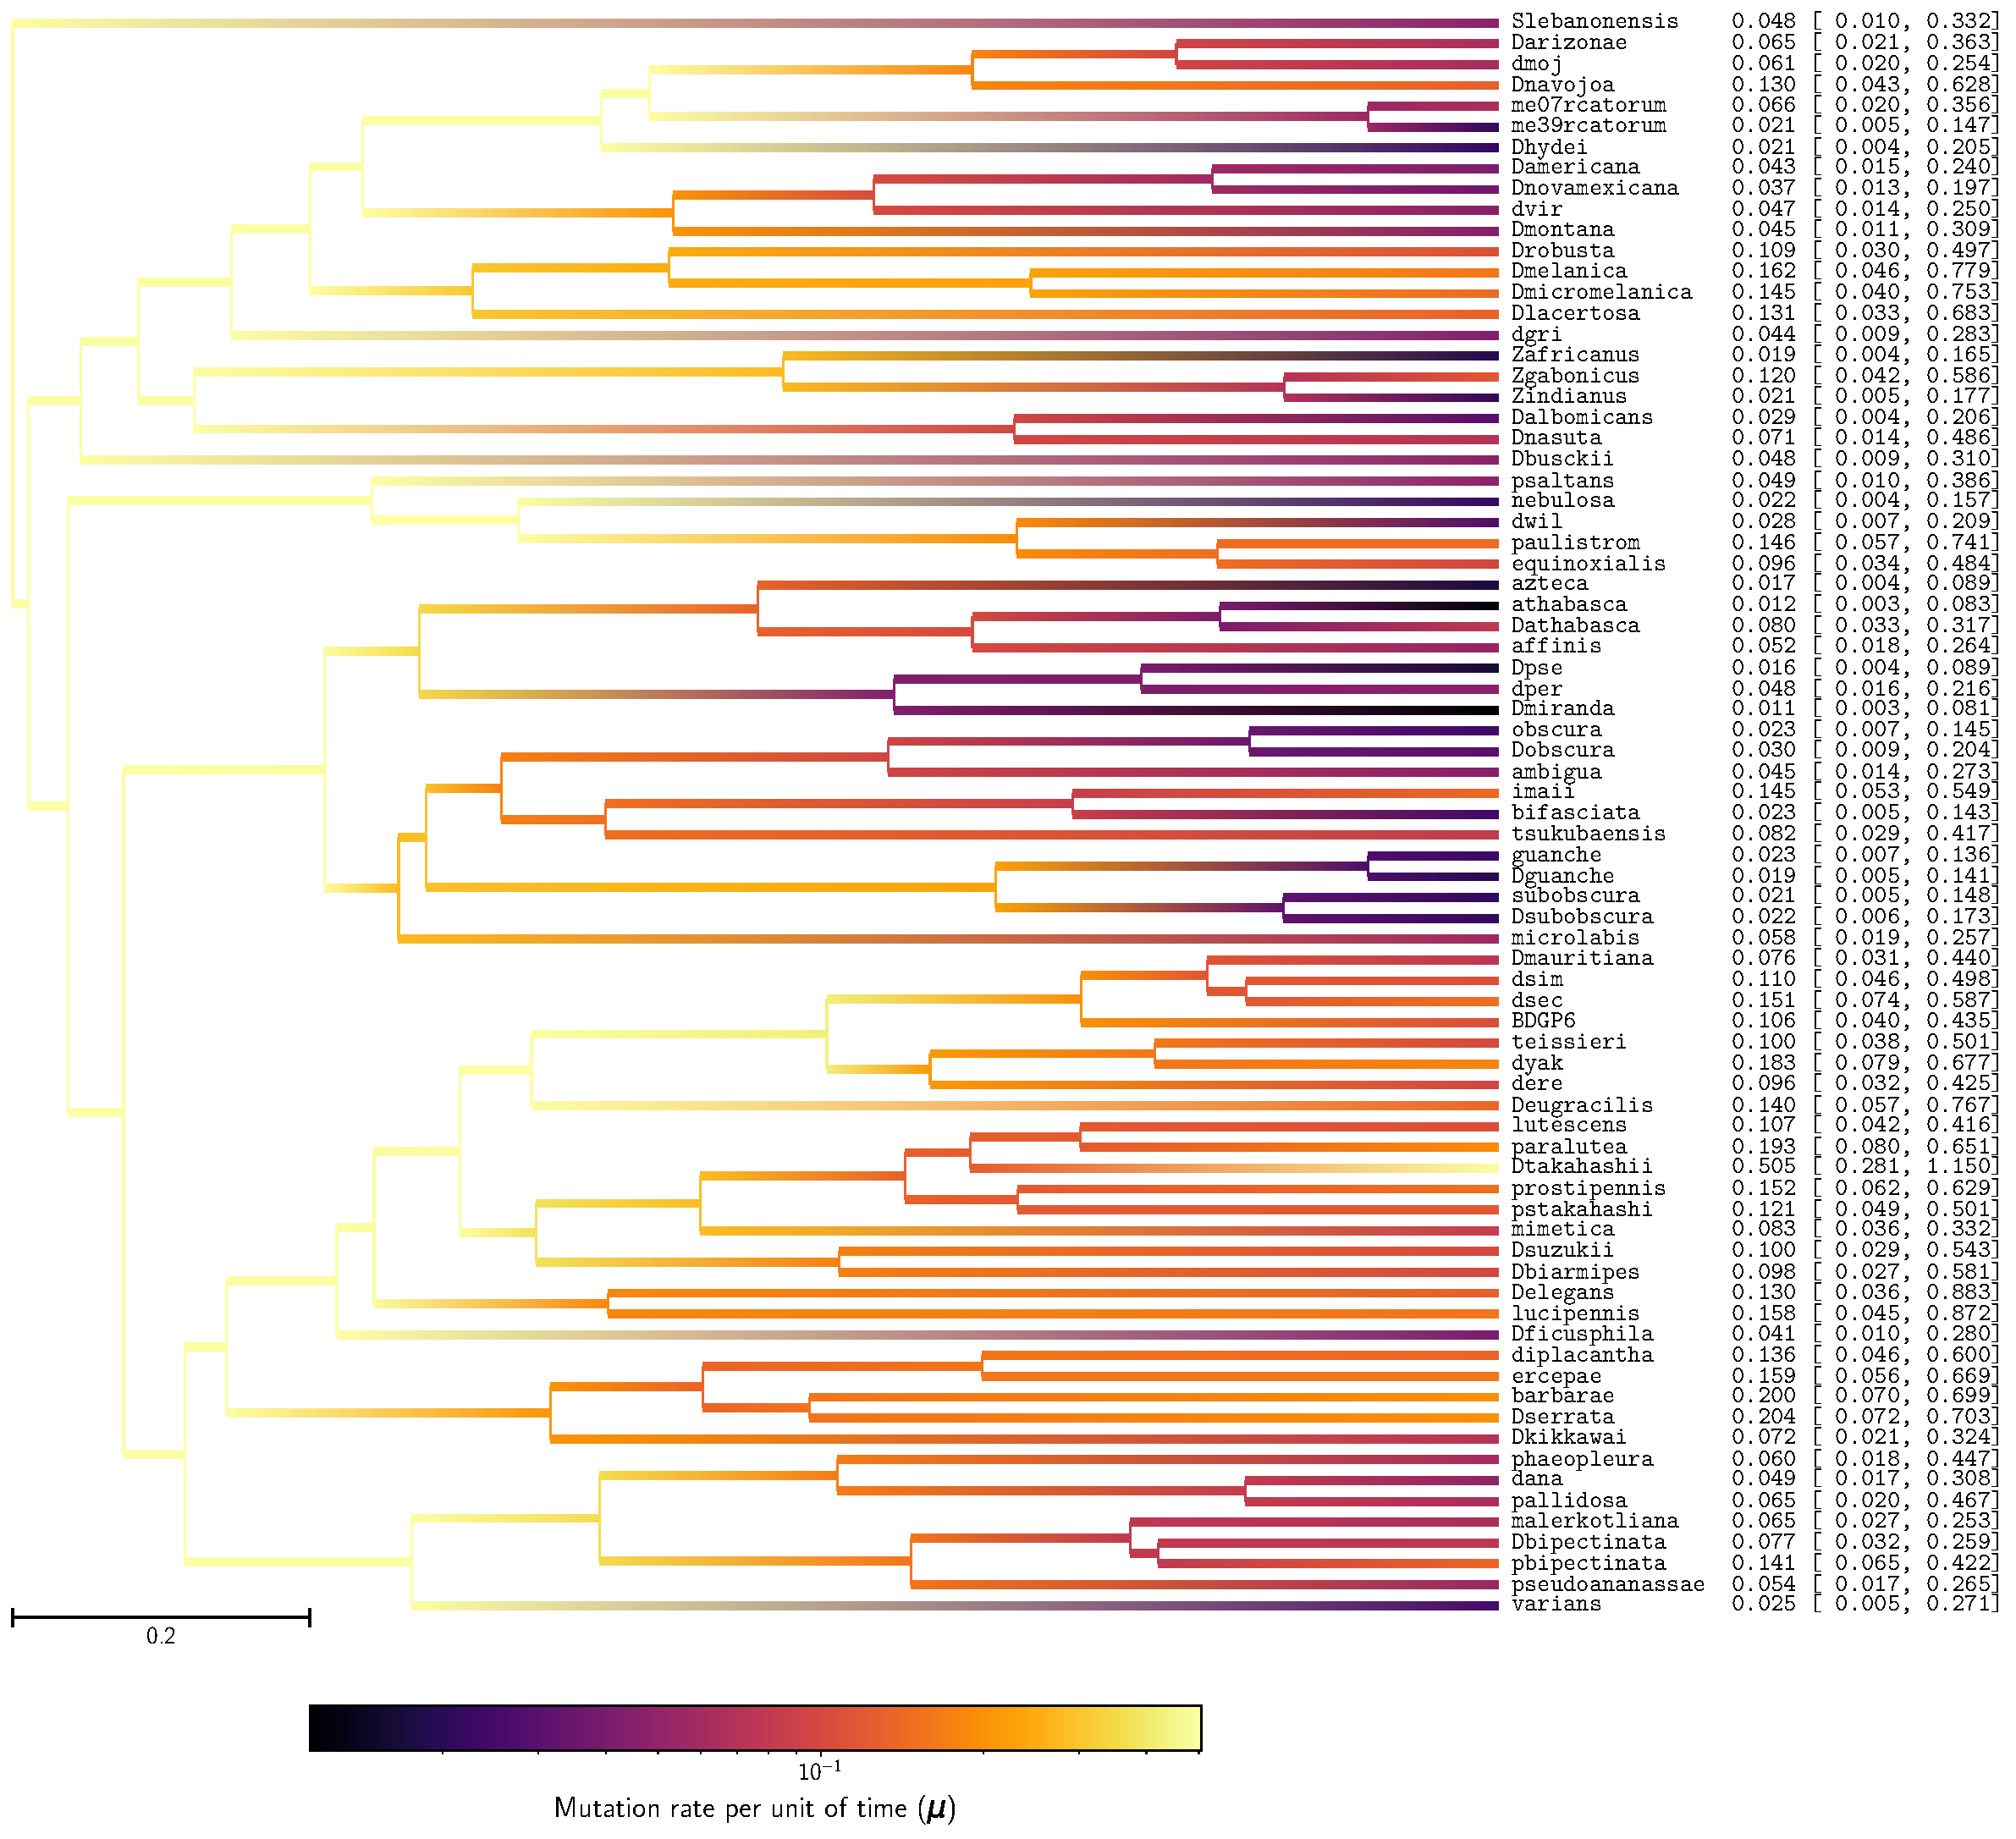
\includegraphics[valign=t, width=\linewidth, page=1, clip, trim=0cm 4.48cm 15.35cm 0cm]{mammals/18CDS_SiteMutSelBranchNe_R1_LogMutationRatePerTime}}
		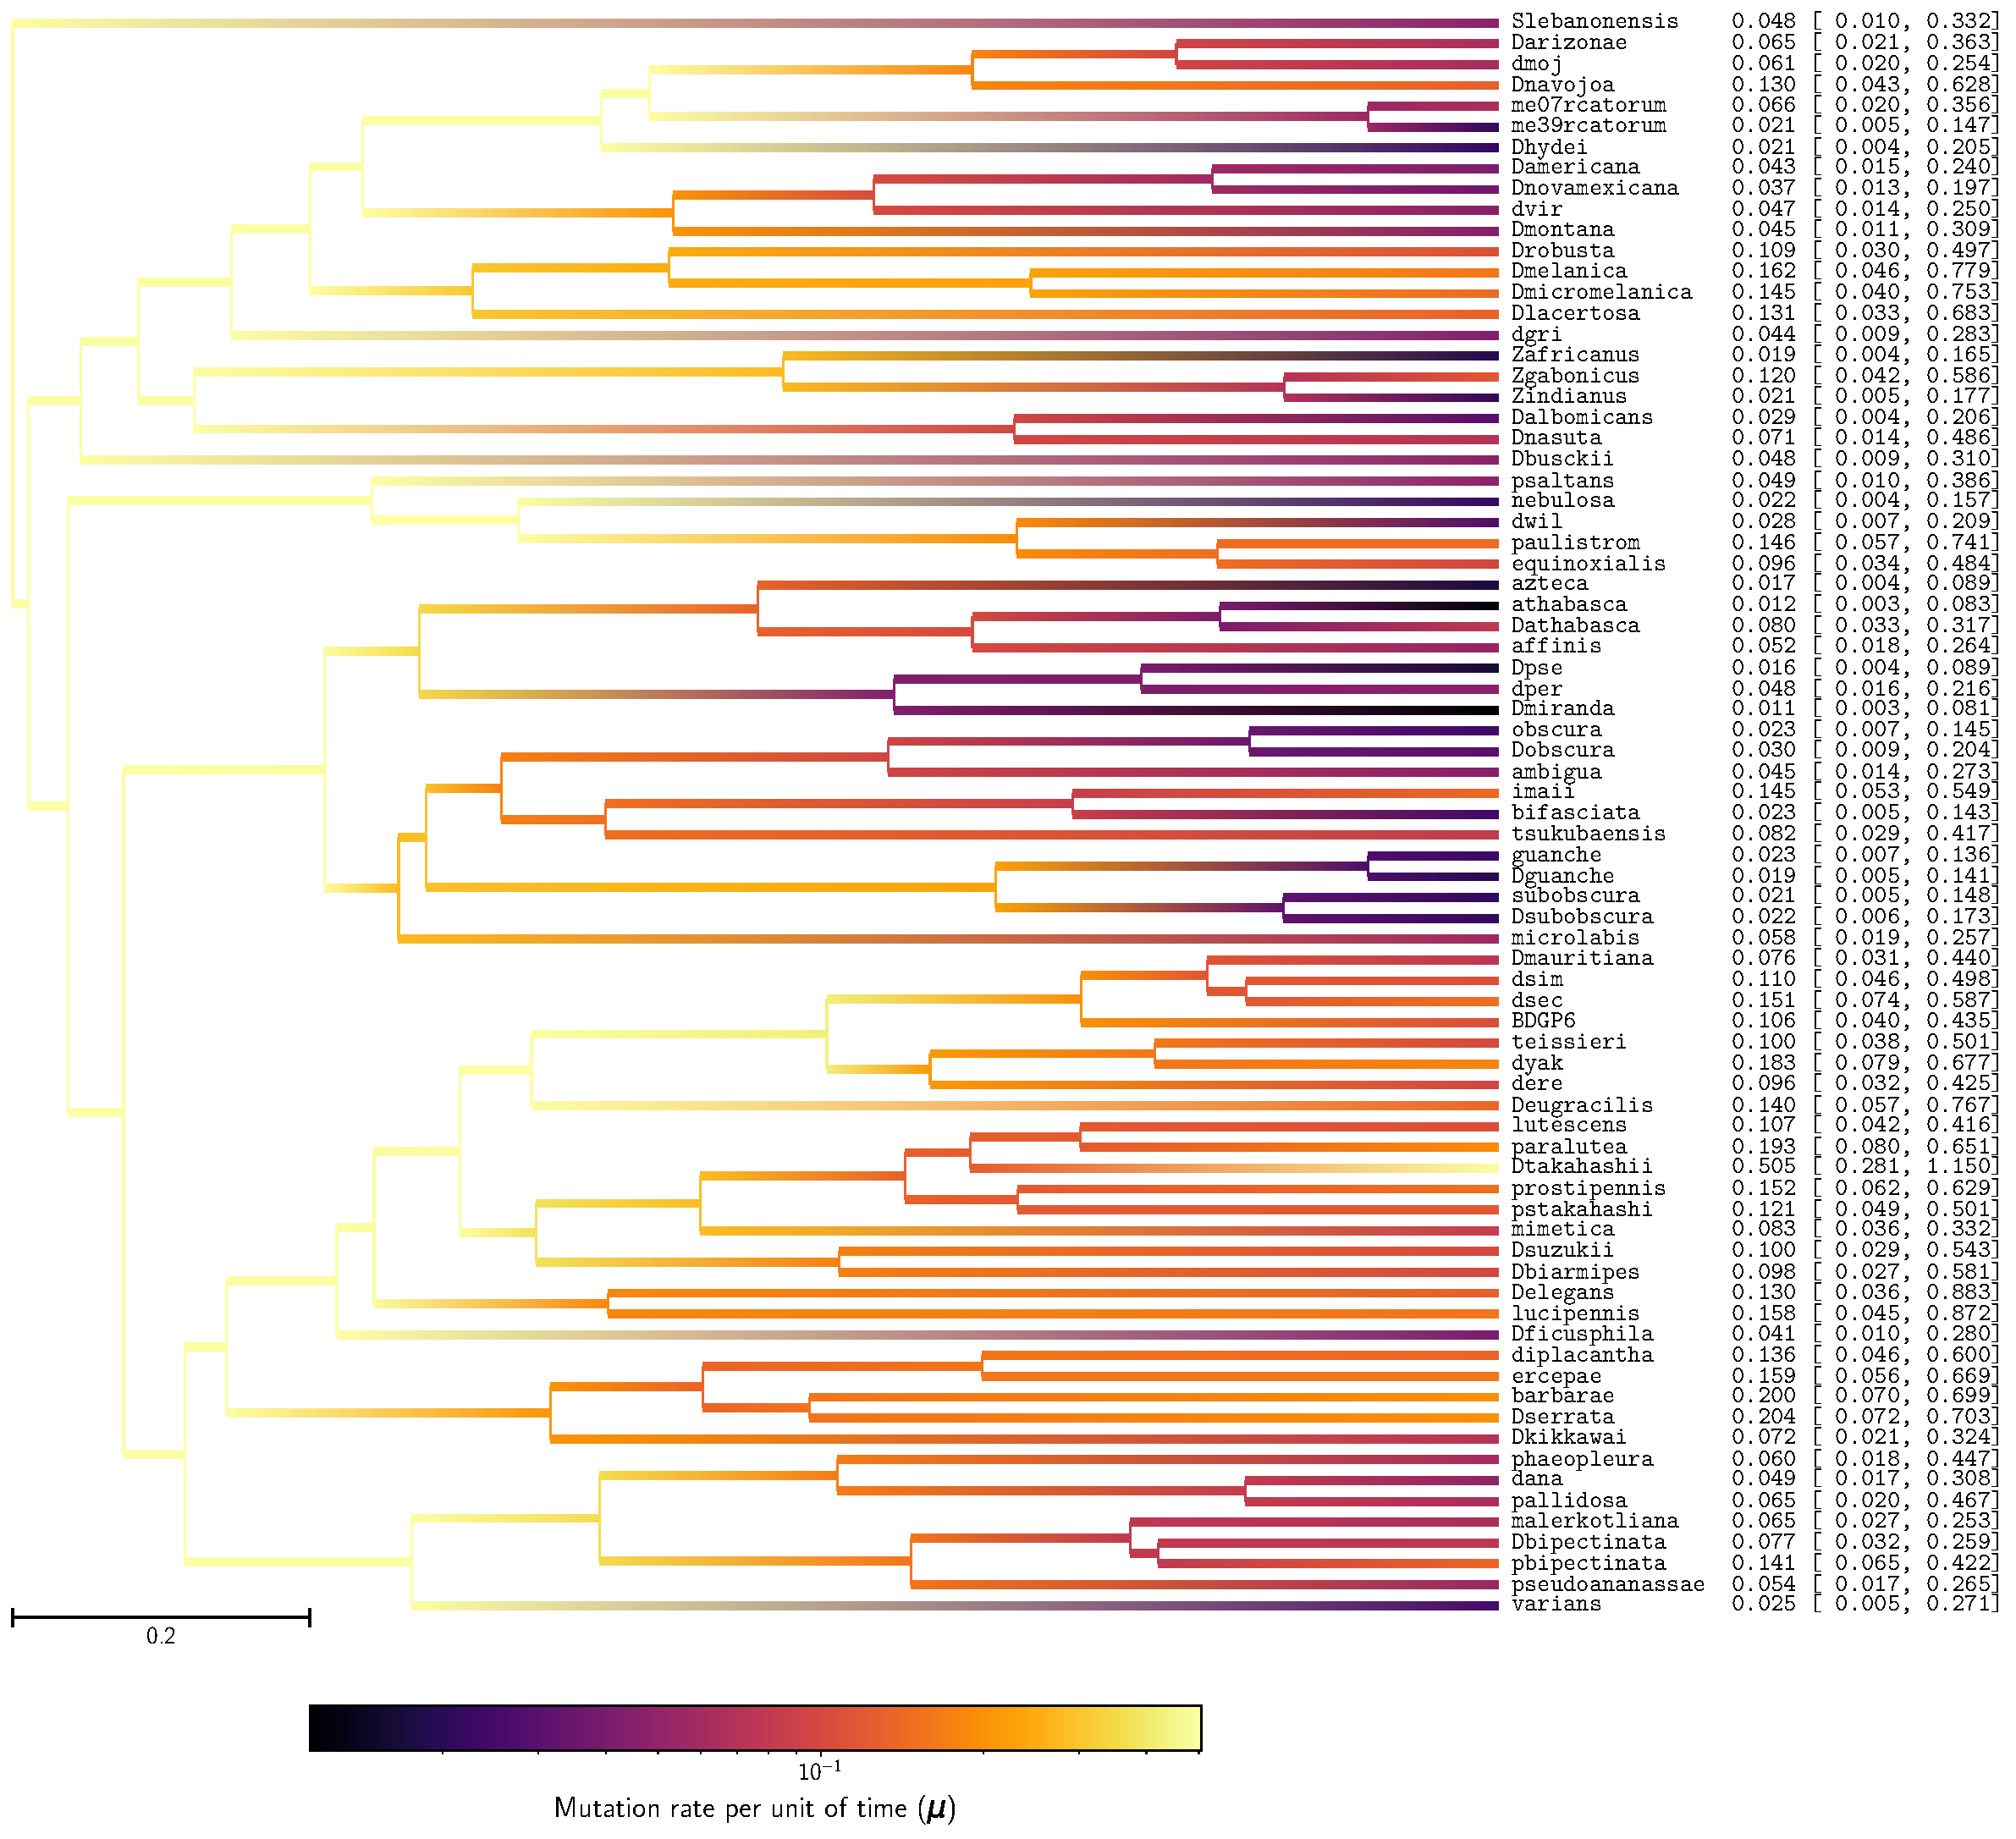
\includegraphics[valign=b,width=\linewidth, page=1, clip, trim=0cm 0cm 15.35cm 32.3cm]{mammals/18CDS_SiteMutSelBranchNe_R1_LogMutationRatePerTime}
	\end{minipage}
	\caption[Example of inferred $\Ne$ and $\mu$ on placental mammals dataset]{
		Example of inferred $\Ne$ and $\mu$ on placental mammals dataset.
		Inference were performed on a randomly chosen set of $36$ coding sequences (CDS) out of $226$ highly conserved CDS~($<1\%$ of gaps).
		Only highly conserved CDS were retained such that the assumption of constant fitness landscape is not incautiously broken by protein with changing function and/or adaptive selection.
		Brownian processes along the tree are represented for effective population size~($\Ne$, left panel) and mutation rate per site per unit of time~($\mu$, right panel).
		Mean values of \acrshort{MCMC} (after burn-in) are obtained at each node of the tree, hence a gradient can be extrapolated along each branch.
		At each node, the inner circle represent the lower bound of the \acrshort{MCMC} $90\%$ confidence interval, and the outer circle represent the upper bound, as to give visual input into the range of estimation.
		$\mu$ spanned almost $2$ order of magnitude, and if we assume the root to be $105$My old \citep{Kumar2017}, the re-scaled mutation rate per site per year in extant species is between $\smash{1.1e^{-10}}$ and $\smash{7.8e^{-9}}$.
		$\Ne$ at the root of the tree is arbitrarily set to $1$, and all values are relative to the root.
	}
	\label{fig:mammals_popsize_and_mutrate}
\end{figure}

We reconstructed long-term changes of effective population size~($\Ne$) and mutation rate per site per unit of time~($\mu$) in placental mammals, with alignments extracted from OrthoMam database \citep{Ranwez2007,Scornavacca2019}.
Life-history traits (LHT) for longevity, age at maturity and weight were obtained from AnAge database \citep{DEMAGALHAES2009,Tacutu2012}.
We focused our analysis on 77 taxa for which information is available for at least one LHT.

In the result of this analysis (Figure~\ref{fig:mammals_popsize_and_mutrate}), we visually observe a global trend of increased $\Ne$ throughout the tree around $90$ and $60$ My.
We also observe $\Ne$ to be lower in \textit{Cetacea} and \textit{Camelidae}, while being higher in \textit{Rodentia} and \textit{Pecora}.
In some clades we can see a decrease along a single branch of the tree, for example \textit{Heterocephalus glaber} or \textit{Acinonyx jubatus}.

The analysis of the covariance matrix, discarding phylogenetic inertia, shows that $\Ne$ is positively correlated~($r^2 = 0.44$) with mutation rate per unit of time (Table~\ref{fig:mammals_correlation}), which is compatible with the assumption that large population are small-sized and with a shorter generation time.
Moreover the \gls{effective-population-size} is negatively correlated with longevity, age at maturity and weight (Table~\ref{fig:mammals_correlation}), consistent with the observation that larger population have small-sized and short-lived individuals \citep{Galtier2016,Romiguier2014}.
The partial-correlation coefficients (Supplementary Materials) are not significantly different from $0$.

However, if the trend of $\Ne$ would be in the right direction, the magnitude of inferred $\Ne$ is vastly underestimated by our method, with a ratio of $2.5$ between the maximum and minimum $\Ne$ in extant species (Figure~\ref{fig:mammals_popsize_and_mutrate}).

To assess the reproducibility of our inference, we analyzed a concatenated random sample of 36 highly conserved coding sequences~($\leq 1\%$ of gaps in the alignment), and repeated the procedure on different random samples of 36 CDS.
Overall the estimation of $\Ne$ is reproducible for a random subset of CDS (Figure~\ref{fig:mammals_repeatability}).

\begin{table}[H]
	\centering
\noindent\adjustbox{max width=\textwidth}{%
\begin{tabu}{|c||c|c|c|}
\hline
\textbf{Correlation ($\bm{\rho}$)} & $\bm{N_{\mathrm{e}}}$ & $\bm{\mu}$ & \textbf{LogGenomeSize}\\
\hhline{|=#=|=|=|}
$\bm{N_{\mathrm{e}}}$ & - & $-0.0623$ & $-0.144$\\\hline
$\bm{\mu}$ & - & - & $0.224$\\\hline
\textbf{LogGenomeSize} & - & - & -\\\hline
\end{tabu}}

	\caption[Traits correlation]{
		Correlation coefficient between effective population size~($\Ne$), mutation rate per site per unit of time~($\mu$), and life-history traits (Maximum longevity, adult weight and female maturity), taking account phylogenetic inertia.
		Correlation coefficient are between $-1$ and $1$.
		Asterisks indicate strength of support~($\smash{^{*}} pp > 0.95$, $\smash{^{**}} pp > 0.975$).
		Observed correlation are compatible with the interpretation that large populations are composed of small, short-lived individuals.
		Moreover if the mutation rate per generation is considered constant in first approximation, the mutation rater per unit of time is positively correlated to generation rate, hence to population size.
	}
	\label{fig:mammals_correlation}
\end{table}

\section{Discussion}
\label{sec:Discussion}
% Summary 
Mechanistic phylogenetic \gls{codon} models explicitly define the \gls{substitution} rates as function of the mutation rate, selection and random drift.
Applied on an alignment of \acrshort{DNA} coding sequence, the mechanistic model can estimate amino-acid fitness landscapes along the \acrshort{DNA} sequence.
On the other hand, molecular comparative framework reconstruct the joint evolution of life-history, molecular and population-genetic traits along the phylogeny, intrinsically including phylogenetic inertia.
Combined together, the resulting framework can reconstruct site-heterogeneous amino-acid fitness landscapes, also the age of internal nodes, and finally reconstruct branch-heterogeneous life-history traits, $\mu$ and $\Ne$, with their correlation.
Testing the method against simulated alignments suggests the signal is strong enough in protein coding \acrshort{DNA} alignment to infer selection at the site level, and long-term changes in $\Ne$ and $\mu$ using a phylogenetic approach.
In placental mammals, $\Ne$ correlates negatively with longevity, weight and maturity, and positively with $\mu$.
Our observations suggest that the empirical signal is strong enough such that we can infer the directional trends in changes.

% Longvariance in Ne 
If the trend is in right direction, the magnitude of the change is greatly inferior to independent estimates.
Different mechanism not accounted for by the model could explain such a low variance of $\Ne$ inferred.
First, genetic hitch-hiking, Hill-Robertson interference, and short-term fluctuations of $\Ne$ could generate this effect.
However, inference on simulations tends to show their effect is not strong enough in the regimes explored.
Second, $\mu$ and $\Ne$ could also be fluctuating along the genome.
This assumption needs to be tested, though we expect that relaxing this assumption would not change drastically the magnitude of inferred $\Ne$.
Third, the \acrshort{DNA} sequences could also be misaligned in some sites, an effect we can control since the inferred $\Ne$ are repeatable for different set of genes.
Fourth, the genes selected in our alignments could be under adaptive evolution, or their function could have changed.
More precisely, the fitness profile at each site could change with time, either due to Red-Queen dynamics or due to epistasis because amino-acid \glspl{substitution} occurred at other sites.
Simulation of \acrshort{DNA} coding sequences under an epistatic landscape seemingly points to epistasis being the principal factor to be investigated, since $\Ne$ could not be appropriately inferred in such a case.
Independently, the magnitude of inferred $\Ne$ is quite similar for the placental mammals dataset and the primates dataset, while we would expect a greater discrepancy at longer phylogenetic scale.
An explanation could be that epistasis is more prevalent at longer time-scale, because the total number of \glspl{substitution} from root to leaves is greater, hence the fitness landscape is less stable.
Thought modeling epistasis in an inference framework is a complex biological, mathematical and computational problem, this work points to a potential signal of epistasis that could be retrieved in phylogenetic context.
% None equilibrium properties 

% Perspective : \gls{codon} bias
Our model also assume no bias in \gls{codon} usage, though the strength of selection for a particular \gls{codon} (or set of codons) among all synonymous possible \glspl{codon} has been proved to be substantial \citep{Plotkin2011}.

This assumption can be relaxed by implementing \gls{codon} preferences that are shared across all sites, such that $41$ more parameters would be required in total.
Such implementation would provide the advantage of estimating \gls{codon} usage biases, and of accounting for its confounding effect while estimating selection and $\Ne$.

% Perspective: 
Bayesian computation shown in this study are based on relatively small alignments~($20,000$ sites at most), and with a limited parametrization in the number of fitness profile categories~($50$).
Analyzing execution duration of the program (not shown) leads to conclude that the number of fitness profile categories is the limiting step to expand the computation.
To estimate genome-wide $\Ne$, we could develop an extended version leveraging parallel computing, where each coding sequence has its own computing process and own profile categories, but the $\Ne$ would be shared by all computing processes.
By increasing the number of categories per site, the magnitude of inferred $\Ne$ would also increase, since fitness profiles would be sharper.

% Perspective: increase power
Mutation-selection models originated with the aim of increasing the power to detect adaptive evolution, by modeling explicitly the confounding effect of purifying selection.
However, by assuming constant $\Ne$ along a phylogeny, the statistical power to detect sites under adaptive evolution is not optimal.
Fitness profiles estimated are averaged along the phylogeny and are more seemingly \gls{neutral} than our estimated profiles under our present framework (Supplementary Materials).
Even though our method requires more computing resources to estimate fitness profiles, it provides a better null model of purifying selection to test against the presence of adaptive evolution.

% Comparison with other methods
Other methods have recently been developed to reconstruct phylogenetic changes in $\Ne$.
For example, a new method (preprint) uses \acrshort{DNA} coding sequences, a distribution of fitness effects, polymorphism and generation-time for some present-day species to reconstruct $\Ne$ along the phylogeny \citep{Brevet2019}.
This method also based on the quasi-neutral theory of evolution allows to estimate the absolute value of $\Ne$, even for species where the polymorphism is unavailable.
Here our method requires neither generation time nor polymorphism, and the fitness effects are not constrained to a specific distribution.
However, the inferred values are solely relative and the computation requires more computing resources.
% Perspective: Short and long-term Ne

Estimating $\Ne$ in a mutation-selection phylogenetic model relies on the relation between $\Ne$ and relative strength of drift, where ultimately the signal of drift comes from the relative rate of \glspl{substitution}.
However, they do not leverage a second aspect of $\Ne$ at the population level, which determines the \gls{neutral} genetic diversity that can be maintained~($\pi=4\Ne \mu \tau$, where $\tau$ is the generation time).
Hence, \gls{polymorphic} data give us independent empirical estimates of $\Ne$, based on the assumption that mutations are \gls{neutral}.
In principle, our mechanistic model could be extended to leverage polymorphism within species in the case of differential selection, a method which has been previously pioneered in the case of $3$ species and using a distribution of fitness effect \citep{Wilson2011}.
More generally, the \gls{nearly-neutral} theory of evolution defines a long-term $\Ne$, which might be different from the short-term definition of $\Ne$ \citep{Platt2018}.
Thus we could ask if empirical independent estimations of $\Ne$ from within species (polymorphic diversity) and between species (\glspl{substitution}) are congruent, and if not what are the mechanisms responsible for this discrepancy.

% Relation to ecology
Notwithstanding theoretical considerations on the quasi-neutral theory of evolution, empirical clues about the long-term trends in the direction of random drift, and changes between species allows to open a large diversity of ecological and evolutionary questions.
Spatial and temporal changes of random drift along ecological niches and events can be investigated to disentangle the underlying evolutionary and ecological pressures.

\begin{figure}[H]
	\centering
	\begin{minipage}{0.32\linewidth}
		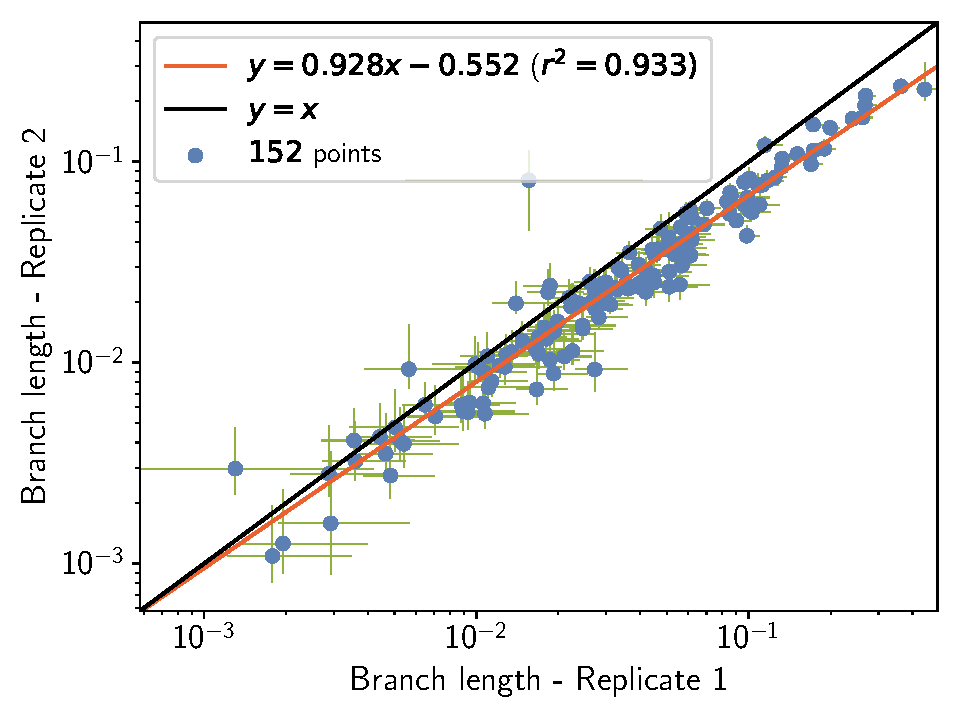
\includegraphics[width=\linewidth, page=1]{mammals/18CDS_SiteMutSelBranchNe_Rep_Log10BranchLength-1-2}
	\end{minipage}	\hfill
	\begin{minipage}{0.32\linewidth}
		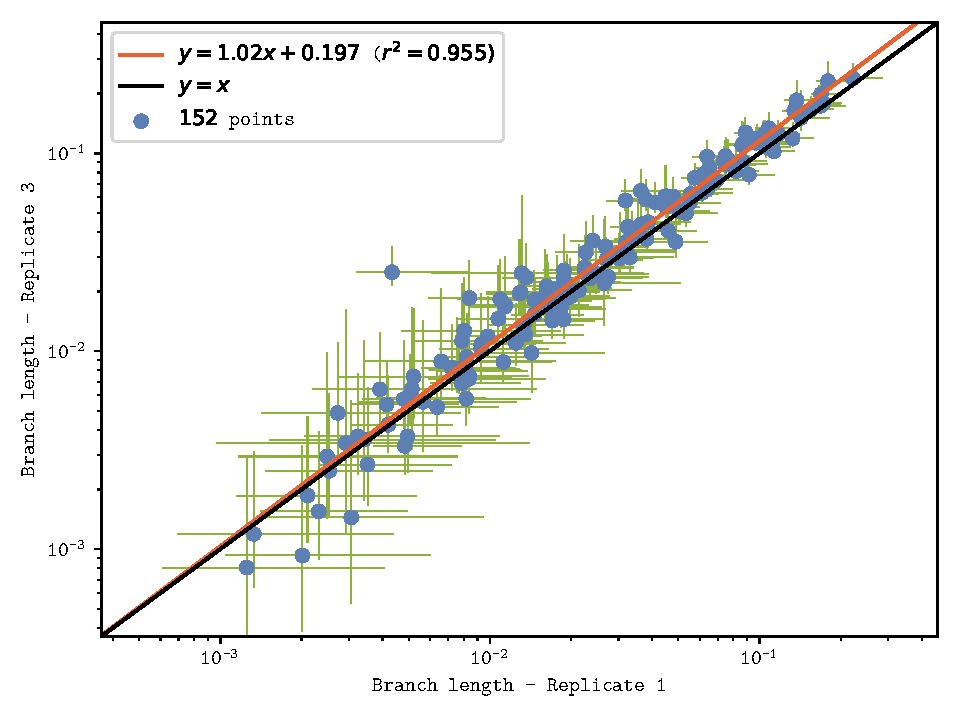
\includegraphics[width=\linewidth, page=1]{mammals/18CDS_SiteMutSelBranchNe_Rep_Log10BranchLength-1-3}
	\end{minipage}	\hfill
	\begin{minipage}{0.32\linewidth}
		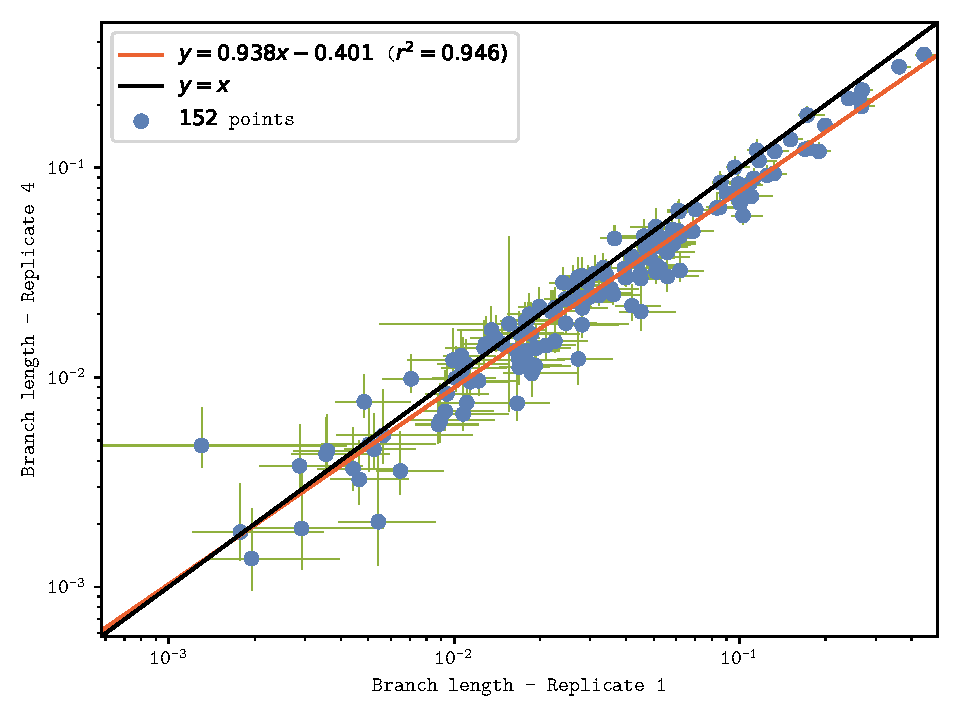
\includegraphics[width=\linewidth, page=1]{mammals/18CDS_SiteMutSelBranchNe_Rep_Log10BranchLength-1-4}
	\end{minipage}
	\begin{minipage}{0.32\linewidth}
		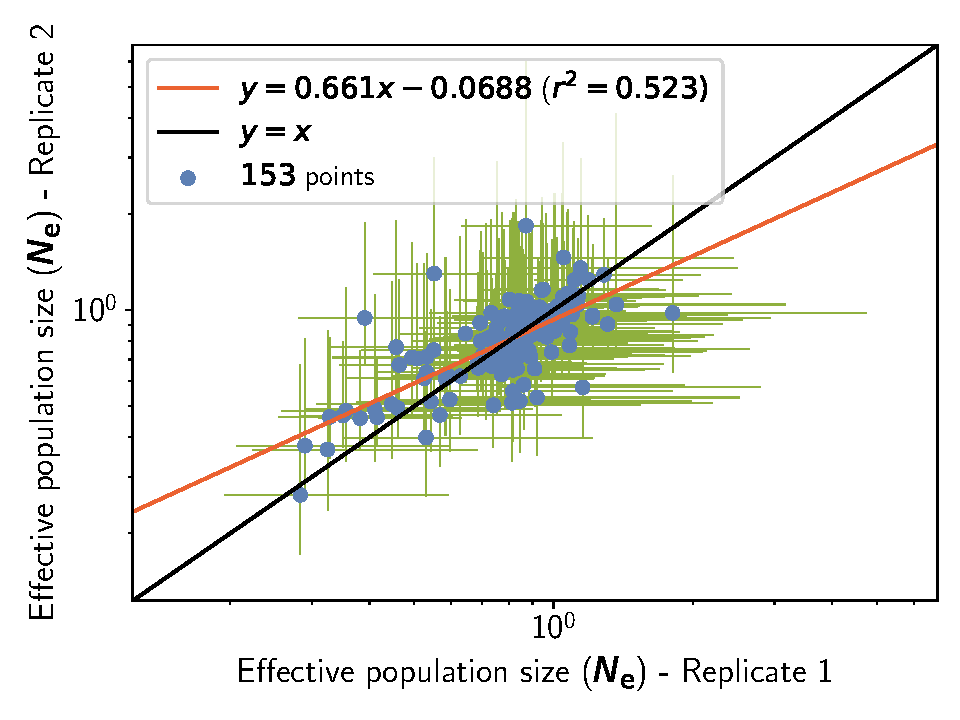
\includegraphics[width=\linewidth, page=1]{mammals/18CDS_SiteMutSelBranchNe_Rep_LogPopulationSize-1-2}
	\end{minipage}	\hfill
	\begin{minipage}{0.32\linewidth}
		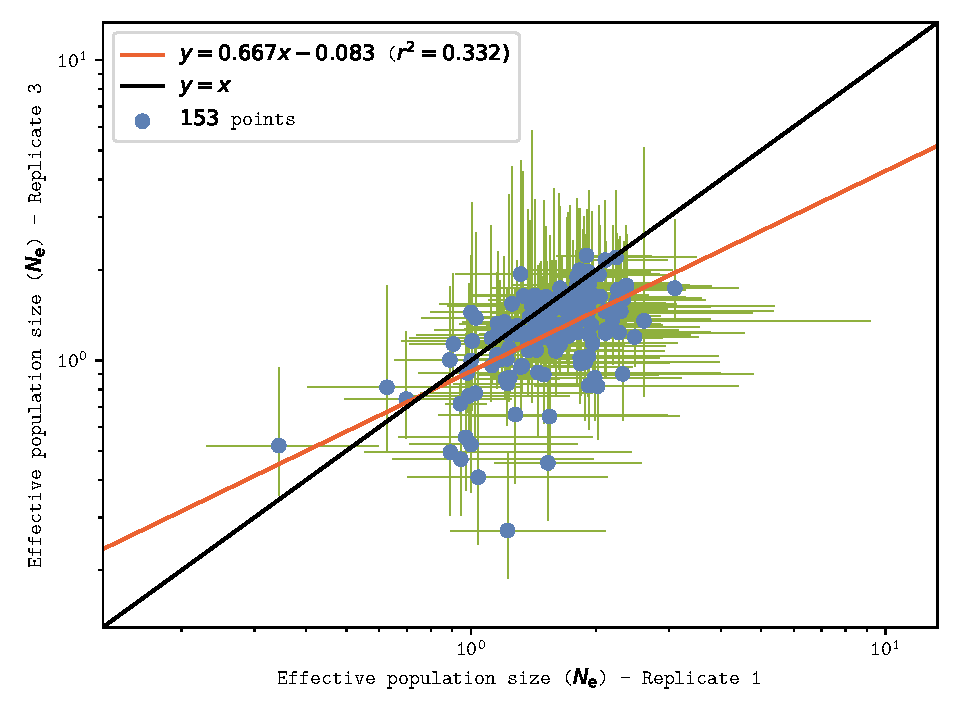
\includegraphics[width=\linewidth, page=1]{mammals/18CDS_SiteMutSelBranchNe_Rep_LogPopulationSize-1-3}
	\end{minipage}	\hfill
	\begin{minipage}{0.32\linewidth}
		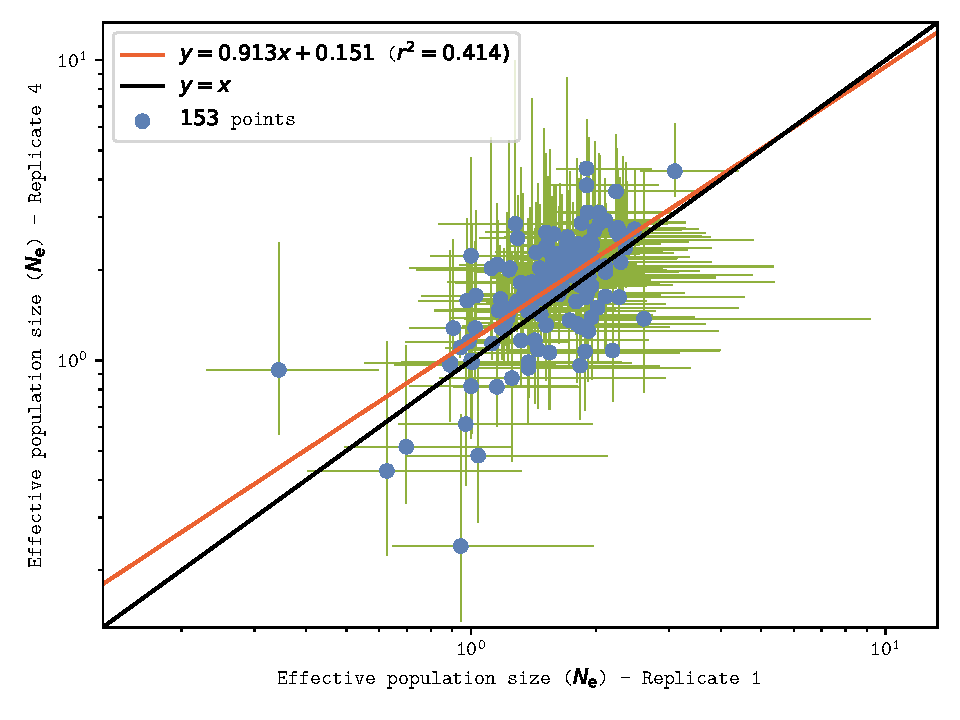
\includegraphics[width=\linewidth, page=1]{mammals/18CDS_SiteMutSelBranchNe_Rep_LogPopulationSize-1-4}
	\end{minipage}
	\caption[Repeatability of experiments]{
		Repeatability of experiments.
		$3$ independent inferences where performed on a randomly chosen set of $36$ coding sequences (CDS) out of $226$.
		Each plot is a correlation between a pair of experiments for a given parameter.
		$2$ relevant parameters are shown, mutation rate per unit of time~($\mu$, bottom left plots) and effective population size~($\Ne$, upper right plots).
		For each node of the tree, the mean of the parameter~($\Ne$ or $\mu$) over the \acrshort{MCMC} is represented in blue dot, green solid lines are the $90\%$ confidence interval of the \acrshort{MCMC}.
		Solid red line is the regression line between experiments.
		Inference of $\mu$ is more reproducible than $\Ne$, but overall the experiment is reproducible for a random subset of CDS.
	}
	\label{fig:mammals_repeatability}
\end{figure}

\section{Materials and Methods model}
\label{sec:MatMet}

\subsection{Nucleotide mutation rates}
The generalized time-reversible nucleotide mutation rate matrix $\Mutmatrix$ is a function of the nucleotide frequencies $\Mutequi$ and the relative rate $\Exchan$.
$\Mutequi = (\mutequi_A , \mutequi_C , \mutequi_G , \mutequi_T)$ is the equilibrium base frequency vector, giving the frequency at which each base occurs at each site.
$\Exchan = \left( \exchan_{AC}, \exchan_{AG}, \exchan_{AT}, \exchan_{CG}, \exchan_{CT}, \exchan_{GT}\right)$ is the vector of exchangeabilities between nucleotides.
Altogether, the rate matrix is:
\begin{equation}
\label{eq:gtr-mutrates}
\Mutmatrix = \begin{pmatrix}
- & {\exchan_{AC} \mutequi_C} & {\exchan_{AG}\mutequi_G} & {\exchan_{AT}\mutequi_T} \\ 
{\exchan_{AC}\mutequi_A} & - & {\exchan_{CG}\mutequi_G} & {\exchan_{CT}\mutequi_T} \\ 
{\exchan_{AG}\mutequi_A} & {\exchan_{CG}\mutequi_C} & - & {\exchan_{GT}\mutequi_T} \\ 
{\exchan_{AT}\mutequi_A} & {\exchan_{CT}\mutequi_C} & {\exchan_{GT}\mutequi_G} & - 
\end{pmatrix},
\end{equation}
By definition, the sum of the entries in each rows of the nucleotide rate matrix $\Mutmatrix$ is equal to $0$, giving the diagonal entries:
\begin{equation}
\mutmatrix_{a,a} = - \sum_{ b \neq a} \mutmatrix_{a,b}
\end{equation}
The \gls{prior} on the exchangeabilities $\Exchan$ is a uniform Dirichlet distribution of dimension $6$:
\begin{equation}
\label{eq:DistribExchan}
\Exchan \sim \mathrm{Dir}\left( \dfrac{1}{6} , 6\right).
\end{equation}
The \gls{prior} on the equilibrium base frequencies $\Mutequi$ is a uniform Dirichlet distribution of dimension $4$:
\begin{equation}
\label{eq:DistribMutequi}
\Mutequi \sim \mathrm{Dir}\left( \dfrac{1}{4} , 4\right)
\end{equation}
The general time-reversible nucleotide matrix is normalized such that the total flow equals to $1$:
\begin{equation}
\sum_{a \in \{A, C, G, T\}} - \mutequi_a \mutmatrix_{a,a} = 1.
\end{equation}

\subsection{Site-dependent selection}
\label{sec:profiles}
For each category $\Setcat$, a $20$-dimensional fitness profile $\Base\catexp$ (summing to $1$) is distributed as a Dirichlet of center $\Basecenter$ and concentration $\baseconc$:
\begin{equation}
\label{eq:DistribBase}
\Base\catexp \sim \mathrm{Dir}\left( \Basecenter,\ \baseconc \right),\ \Setcat.
\end{equation}
For an alignment of size $\Nsite$, each site $\Setsite$ is assigned a fitness profile category of amino-acids $\catsite \in \catInterval $.
The total number of sites falling in each fitness profile category $\cat$ is denoted $\catmultivar_{\cat}$.
The $\Ncat$-dimensional vector $\catMultiVar$ is distributed as a Multinomial of event probabilities $\StickBreaking$:
\begin{align}
\label{eq:DistribMultinomial}
\catMultiVar \sim \mathrm{Multinomial}\left( \StickBreaking \right).
\end{align}
The event probabilities $\Ncat$-dimensional vector~($\StickBreaking$) of falling into each category is distributed as a stick-breaking \gls{Dirichlet-process}:
\begin{align}
\label{eq:DistribStickBreaking}
\begin{split}
& \StickBreaking \sim \mathrm{StickBreaking}\left( \Ncat, \stickbreakinghyper \right)\\
\iff & \stickbreaking_{\cat} = \stick_{\cat}\cdot \prod _{{\indice=1}}^{{\cat-1}}\left(1-\stick_{\indice}\right),\ \Setcat,
\end{split}
\end{align}
where $\stick_{\cat}$ are i.i.d.
from a beta distribution
\begin{equation}
\label{eq:Beta}
\stick_{\cat} \sim \mathrm{Beta}\left( 1, \stickbreakinghyper \right),\ \Setcat.
\end{equation}
The Malthusian fitness selection coefficients $\Fit\siteexp$ at site $\site$, are obtained by taking the logarithm of the fitness profile assigned to this site:
\begin{equation}
\label{eq:sitefitness}
\Fit\siteexp = \log \left( \Base^{\left( \catsite \right)} \right),\ \Setsite.
\end{equation}

\subsection{Dated tree}
The topology of the rooted phylogenetic tree is supposed to be known and is not estimated by the model. The model estimates the dates at which branches split, thus the dated tree requires $\Ntaxa - 2$ internal node ages that are free parameters, where $\Ntaxa$ is the number of extant taxa (leaves of the tree). 
The node ages $\age\nodeexp,\ \Setinternal$ are drawn uniformly such that a node can not be younger than the oldest of its $2$ descendant children, and must also be younger than its parent:
\begin{equation}
\label{eq:Distribage}
\age\nodeexp \ \sim \mathcal{U}\left( \mathrm{max}\left(\age^{(\mathrm{children})} \right), \age^{(\mathrm{parent})} \right)
\end{equation}
By definition, leaf ages are all set to $0$. The root age is set arbitrarily to $1$, but if fossils data are also available the dated tree can be re-scaled into absolute time using cross-multiplication.\\
The duration of the branch~($\branchtime\branchexp$), for each branch $\Setbranch$ is defined as the difference in ages between the oldest node at the tip of the branch $\age^{(\nodeUp)}$, and the youngest node $\age^{(\nodeDown)}$:
\begin{equation}
\label{eq:ageTobranchtime}
\branchtime\branchexp = \age^{(\nodeUp)} - \age^{(\nodeDown)}.
\end{equation}
\subsection{Branch dependent traits}
The \gls{effective-population-size} $\Ne$ and mutation rate per unit of time $\mu$ are assumed to evolve along the phylogeny, and to be correlated.
If quantitative life-history-traits (LHT) are also available for some nodes of the tree (leaves and/or internal nodes), they are also assumed to evolve along the phylogeny and to be correlated between them, and with $\Ne$ and $\mu$.
The total number of traits (counting $\Ne$, $\mu$ and all user defined LHT) is denoted $\Ntrait$.
Their fluctuations are modelled by a $\Ntrait$-dimensional log-Brownian process $\Brownian\nodeexp$ at each node $\Setnode$ of the tree, including the root and leaves.
The first dimension (indiced by $0$) of the log-Brownian contain $\Ne$, and the second dimension (indiced by $1$) contains $\mu$.
The log-Brownian process and variables of interest~($\mu$ and $\Ne$) are linked by an exponential transformation:
\begin{equation}
\begin{dcases}
\Ne\nodeexp = \e^{ \brownian_{0}\nodeexp } \\ 
\mu\nodeexp = \e^{ \brownian_{1}\nodeexp },
\end{dcases}
\end{equation}
where the \gls{effective-population-size} at the root is set to $1$ for identifiability of the fitness profiles.
It is important to note that inferred correlation between $\Ne$, $\mu$ and other LHT is thus in the log space, and that quantitative LHT must be inputted in log scale.

Along a branch $\Setbranch$ of the tree, a log-Brownian process starts at the oldest node at the tip of the branch~($\nodeUp$), and ends at the youngest node~($\nodeDown$).
However we are interested in the average over the branch to define the \gls{codon} \gls{substitution} matrices along the branch.
In the case of log-Brownian process, the most likely path (or geodesic) from $\Brownian^{(\nodeUp)}$ to $\Brownian^{(\nodeDown)}$ is the straight line, and therefore, it would make sense to take the mean value of $\e^{\Brownian\nodeexp}$ along this geodesic.
We then have $\Ne\branchexp$ and $\mu\branchexp$ for each branch $\Setbranch$ of the tree:
\begin{equation}
\label{eq:branchNemu}
\begin{dcases}
\Ne\branchexp = \dfrac{\e^{\brownian_{0}^{(\nodeDown)}} - \e^{\brownian_{0}^{(\nodeUp)}}}{\brownian_{0}^{(\nodeDown)} - \brownian_{0}^{(\nodeUp)}} \\ 
\mu\branchexp = \dfrac{\e^{\brownian_{1}^{(\nodeDown)}} - \e^{\brownian_{1}^{(\nodeUp)}}}{\brownian_{1}^{(\nodeDown)} - \brownian_{1}^{(\nodeUp)}}.
\end{dcases}
\end{equation}

Moreover, the rate of change of the log-Brownian process per unit of time is constant and determined by the positive semi-definite and symmetric covariance matrix $\CovarianceMatrix$, and thus the distribution of $\Brownian^{(\nodeDown)}$ is multivariate Gaussian, with mean $\Brownian^{(\nodeUp)}$ and variance $\branchtime\branchexp \CovarianceMatrix$:
\begin{equation}
\label{eq:DistribBrownian}
\Brownian^{(\nodeDown)} \sim \mathcal{N}\left(\Brownian^{(\nodeUp)}, \branchtime\branchexp \CovarianceMatrix \right),\ \Setbranch
\end{equation}

\begin{figure}[H]
	\centering
		\begin{tikzpicture}[->,>=stealth',shorten >=1pt,auto,node distance=0.6cm and 1.2cm,semithick]
		\tikzstyle{every state}=[]
		
		\node[state] (P) {$\Probmatrix\branchsiteexp$};
		\node[state] (Q) [below right=of P] {$\Submatrix\branchsiteexp$};
		\node[state] (R) [below right=of Q] {$\Mutmatrix$};
		\node[state] (BL) [above right=of P] {$\branchlength\branchexp$};
		\node[state] (Ne) [above right=of Q] {$\Ne\branchexp$};
		\node[state] (Bb) [above right=of Ne] {$\Brownian\nodeexp $};
		\node[state] (Mu) [left=of Bb] {$\mu\branchexp$};
		\node[state] (f) [right=of Q] {$\Fit\siteexp $};
		\node[state] (Ex) [BLUE, below right=of R] {$\Exchan$};
		\node[state] (Equi) [BLUE, right=of R] {$\Mutequi$};
		\node[state] (dT) [above left=of Bb] {$\branchtime\branchexp $};
		\node[state] (T) [BLUE, right=of dT] {$\age\nodeexp$};
		\node[state] (Base) [BLUE, above right=of f] {$\Base\catexp$};
		\node[state] (cat) [BLUE, right=of f] {$\catsite$};
		\node[state] (ExH) [RED, right=of Ex] {$\dfrac{1}{6}, 6$};
		\node[state] (EquiH) [RED, right=of Equi] {$\dfrac{1}{4}, 4$};
		\node[state] (Unif) [RED, right=of T] {$\uniform$};
		\node[state] (C) [BLUE, right=of Bb] {$\contrast\branchexp$};
		\node[state] (Cov) [BLUE, right=of C] {$\Covariancematrix$};
		\node[state] (baseH) [RED, right=of Base] {$\baseconc, \Basecenter $};
		\node[state] (sb) [BLUE, right=of cat] {$\StickBreaking$};
		\node[state] (CovH) [RED, right=of Cov] {$\covariancekappa, \covariancedf$};
		\node[state] (sbH) [RED, right=of sb] {$\stickbreakinghyper$};
		
		\path 
		(Q) edge [dashed] node [above right] {\ref{eq:Probmatrix}} (P)
		(dT) edge [dashed] node [above left] {\ref{eq:branchlength}} (BL)
		(Mu) edge [dashed] node [] {} (BL)
		(BL) edge [dashed] node [] {} (P)
		(Ne) edge [dashed] node {} (Q)
		(R) edge [dashed] node {} (Q)
		(Bb) edge [dashed] node {} (Ne)
		(Bb) edge [dashed] node [below] {\ref{eq:branchNemu}} (Mu)
		(f) edge [dashed] node [above] {\ref{eq:subrates}} (Q)
		(Ex) edge [dashed] node [] {} (R)
		(Equi) edge [dashed] node [below] {\ref{eq:gtr-mutrates}} (R)
		(T) edge [dashed] node [above] {\ref{eq:ageTobranchtime}} (dT)
		(dT) edge [dashed] node {} (Bb)
		(Base) edge [dashed] node {} (f)
		(cat) edge [dashed] node [above] {\ref{eq:sitefitness}} (f)
		(ExH) edge [BLUE] node [above] {\ref{eq:DistribExchan}} (Ex)
		(EquiH) edge [BLUE] node [above] {\ref{eq:DistribMutequi}} (Equi)
		(Unif) edge [BLUE] node [above] {\ref{eq:Distribage}} (T)
		(C) edge [dashed] node [above] {\ref{eq:independent_contrast}} (Bb)
		(Cov) edge [BLUE] node [above] {\ref{eq:Distribcontrast}} (C)
		(baseH) edge [BLUE] node [above] {\ref{eq:DistribBase}} (Base)
		(sb) edge [BLUE] node [above] {\ref{eq:DistribMultinomial}} (cat)
		(CovH) edge [BLUE] node [above] {\ref{eq:Distribcovariance}} (Cov)
		(sbH) edge [BLUE] node [above] {\ref{eq:DistribStickBreaking},\ref{eq:Beta}} (sb);
		\end{tikzpicture}

	\caption[Directed acyclic graph of dependencies between variables]{
	Directed acyclic graph of dependencies between variables.
	Nodes of the directed acyclic graph are the variables, and edges are the functions.
	Hyper-parameters are depicted in {\color{RED}{red}} circle, random variables in {\color{BLUE}{blue}} circles, and transformed variables in black.
	Solid {\color{BLUE}{blue}} line denotes a drawing from a random distribution, and black dashed lines denote a function.
}
	\label{fig:graph}%
\end{figure}

We make a change of variable as to define the branch-wise independent contrast $\contrast\branchexp$:
\begin{align}
\contrast\branchexp &= \dfrac{\brownian^{(\nodeDown)} - \brownian^{(\nodeUp)}}{\sqrt{\branchtime\branchexp}} \\
\label{eq:independent_contrast}
\iff \brownian^{(\nodeDown)} &= \brownian^{(\nodeUp)} + \sqrt{\branchtime\branchexp}\contrast\branchexp 
\end{align}
And these contrasts are i.i.d.
from a multivariate normal distribution:
\begin{equation}
\label{eq:Distribcontrast}
\contrast\branchexp \sim \mathcal{N}\left(\bm{0}, \Covariancematrix \right), \Setbranch
\end{equation}
The \gls{prior} on the covariance matrix is an invert Wishart distribution, parameterized by $\covariancekappa=1$ and with $\covariancedf=\Ntrait + 1$ degrees of freedom:
\begin{equation}
\label{eq:Distribcovariance}
\CovarianceMatrix \sim \mathrm{Wishart}^{-1} (\covariancekappa \Identitymatrix, \covariancedf)
\end{equation}

\subsection{Codon \gls{substitution} rates}
For a given branch $\branch$ and a given site $\site$, the \gls{codon} \gls{substitution} rate (per unit of time) matrix $\Submatrix\branchsiteexp$ is given by:
\begin{equation}
\label{eq:subrates}
\begin{dcases}
\submatrix\branchsiteexp_{\itoj} = 0\text{ if $\ci$ and $\cj$ are not neighbors,} \\
\submatrix\branchsiteexp_{\itoj} = \mutmatrix_{\nucitoj}\text{ if $\ci$ and $\cj$ are synonymous,} \\
\submatrix\branchsiteexp_{\itoj} = \mutmatrix_{\nucitoj} \dfrac{4\Ne\branchexp \left({\fitj\siteexp - \fiti\siteexp}\right)}{{1 - \e^{4\Ne\branchexp\left({\fiti\siteexp - \fitj\siteexp}\right)} }} \text{ if non-syn.,}\\
\submatrix\branchsiteexp_{\ci, \ci} = - \sum_{ \cj \neq \ci, \jSetCodon} \submatrix\branchsiteexp_{\itoj},
\end{dcases}
\end{equation}
The branch length $\branchlength\branchexp$ are defined as the expected number of \gls{neutral} \glspl{substitution} per \acrshort{DNA} site along a branch:
\begin{equation}
\label{eq:branchlength}
\branchlength\branchexp = \mu\branchexp \branchtime\branchexp
\end{equation}
Together, the probability of {transition} between \glspl{codon} for a given branch $\branch$ and site $\site$ is:
\begin{equation}
\label{eq:Probmatrix}
\Probmatrix\branchsiteexp = \e^{\branchlength\branchexp \Submatrix\branchsiteexp},
\end{equation}
which are the matrices necessary to compute the \gls{likelihood} of the data $\data$ given the parameters of the model using the pruning algorithm (Supplementary Materials).

\subsection{Bayesian implementation}
\label{sec:Bayesian}
The \gls{likelihood} computed by the pruning algorithm can then be combined with the \gls{prior} over the model parameters.
A realization of the random process results in a detailed \gls{substitution} history over the tree.
Most phylogenetic Monte-Carlo-Markov-Chain (\acrshort{MCMC}) samplers target the distribution over the model parameters, which means that they have to repeatedly invoke the pruning algorithm to recalculate
the pruning-based \gls{likelihood} which is most often the limiting step of the \acrshort{MCMC}.

An alternative, which is used here, is to do the \acrshort{MCMC} conditionally on the detailed \gls{substitution} history $\subhistory$, thus doing the \acrshort{MCMC} over the augmented configuration~($\subhistory$, $\data$), under the target distribution obtained by combining the mapping-based \gls{likelihood} with the \gls{prior} over model parameters

The key idea that makes this strategy efficient is that the mapping-based \gls{likelihood} depends on
compact summary statistics of $\subhistory$ (which in turn depend on the specific parameter component
being resampled), leading to very fast evaluation of the \gls{likelihood}.
On the other hand, this requires to implement more complex \acrshort{MCMC} procedures, that have to alternate between:

1) sampling $\subhistory$ conditionally on the data and the current parameter configuration.

2) re-sampling the parameters conditionally on $\subhistory$.

To implement the mapping-based \acrshort{MCMC} sampling strategy, we first sample the detailed \gls{substitution} history $\subhistory$ for all sites along the tree.
Several methods exist for doing this \citep{Nielsen2002,Rodrigue2008}.
Then, we write down the probability of $\subhistory$ given the parameters, and finally, we collect all factors that depend on some parameter of interest and make some simplifications.
This ultimately leads to relatively compact sufficient statistics (Supplementary Materials for the different sufficient statistics used by our model) that are fast to evaluate \citep{Irvahn2014,Davydov2016}.

As an example, making an \acrshort{MCMC} move on the $\Ne$ at a given node of the tree is drastically faster since only the mapping-based \gls{likelihood} (using path sufficient statistics) at the neighboring branches of the node is necessary, and not computing the \gls{likelihood} for the all tree.
\\

\subsection{Correlation between traits}
\label{sec:Correlation}
The correlation between traits $\Settrait$ and trait $\traitj \in \traitInterval$ can be obtained from the covariance matrix $\Covariancematrix$:
\begin{equation}
\rho_{\traiti, \traitj} = \dfrac{\Covariancematrix_{\traiti, \traitj}}{\sqrt{\Covariancematrix_{\traiti, \traiti} \Covariancematrix_{\traitj, \traitj}}}
\end{equation}

\subsection{Simulations}
\label{sec:Simulation}
To test the robustness of the model, $3$ parameterized simulators were developed: \textit{SimuDiv}, \textit{SimuPoly} \& \textit{SimuFold}.
All $3$ simulators use a log-Brownian multivariate process to model conjointly the changes in mutation rate per generation, the generation time and $\Ne$, in logarithm space.
\textit{SimuDiv} \& \textit{SimuFold} both simulate point \glspl{substitution} along the phylogenetic tree.
The simulator starts from an initial sequence at equilibrium.
The change in fitness is computed for all possible mutant, hence computing all strictly positive \gls{substitution} rates.
At each point, the next \gls{substitution} is chosen proportional to the rate as in Gillespie algorithm.
At each node, the process is split, and finally the process is stopped at the leaves of the tree.
\textit{SimuPoly} simulates explicitly each generation along the phylogeny under a Wright-Fisher population, consisting of three steps: mutation, selection and random drift of \glspl{allele}.
Mutations are drawn randomly based on the probability of mutation.
Drift is modeled as a multinomial distribution on the \gls{allele} counts.
We assumed that the \acrshort{DNA} sequence is composed of exons, with no linkage between exons, and total linkage of sites within an exon.
Moreover, in \textit{SimuPoly} $\Ne$ can also be modeled as a sum of a log-Brownian process and an Ornstein-Uhlenbeck process.
The log-Brownian motion takes into account long-term fluctuations, while the Ornstein-Uhlenbeck can take into account short fluctuations of $\Ne$.
In \textit{SimuDiv} and \textit{SimuPoly} each \gls{codon} site contribute independently to the fitness depending on the encoded amino-acids, through site-specific amino-acid fitness profiles experimentally determined \citep{Bloom2017}.
However, in \textit{SimuFold} the fitness of a sequence is computed as the probability of the protein to be in the folded state (Supplementary Materials).
\textit{SimuFold} is in practice a C++ adaptation of a Java code previously published \citep{Goldstein2016, Goldstein2017}, where we allow for changes in $\Ne$ and $\mu$ along a phylogenetic tree.

The simulators written in C++ are publicly available under MIT license at \url{https://github.com/ThibaultLatrille/SimuEvol}

\section{Acknowledgments}
Supplementary materials deriving mathematical formulas and figures are available at "!!!!TO BE WRITTEN!!!!".
Mammalian alignments and life-history traits, simulated alignments and results of experiments are available at \url{https://datadryad.org/"!!!!TO BE WRITTEN!!!!"}.
The scripts and instructions necessary to reproduce the experiments are available at \url{https://github.com/ThibaultLatrille/MutationSelectionDrift}.


The authors gratefully acknowledge the help of Nicolas Rodrigue, Laurent Guegen, Philippe Veber for their advice and review concerning this manuscript.
This work was performed using the computing facilities of the CC LBBE/PRABI.
A PhD grant of the École normale supérieure de Lyon awarded to T.L.
provided a salary during the work.


\chapter{Supplementary Materials}
{\hypersetup{linkcolor=GREYDARK}\minitoc}
\section{Summary statistics}

\subsection{Partial correlation coefficient}

The correlation coefficient $\rho_{\traiti, \traitj}$ give the total regression between two variables.
Partial-correlation coefficient account for the entire covariance matrix, and measure the correlation between $2$ traits, knowing the values of all the other traits:
\begin{equation}
    \rho_{\traiti, \traitj | c \in \traitInterval \setminus \{ a, b\} } = - \dfrac{\Precisionmatrix_{\traiti, \traitj}}{\sqrt{\Precisionmatrix_{\traiti, \traiti} \Precisionmatrix_{\traitj, \traitj}}},
\end{equation}
where the precision matrix $\PrecisionMatrix$ is the inverse of the covariance matrix:
\begin{equation}
    \PrecisionMatrix = \CovarianceMatrix^{-1}
\end{equation}

\subsection{Fitness profile entropy}
For a category $\cat$, the Shannon entropy ($\entropy$) of the fitness profile is defined as:
\begin{equation}
    \entropy\catexp = - \sum\limits_{\aSetAa} \base\catexp_{\aminoacid} \log \left( \base\catexp_{\aminoacid} \right)
\end{equation}
The Shannon entropy measures the flatness of the fitness profile, with a value of $0$ corresponding to a single peak fitness landscape (only one amino-acid is present), and a value of $log(20)\simeq3$ corresponding to a \gls{neutral} landscape, where each amino-acid has the same fitness.

The Shannon entropy can be averaged over all sites as:
\begin{equation}
    \langle \entropy \rangle = \dfrac{1}{\Nsite}\sum\limits_{\Setsite} \entropy^{\catsite}
\end{equation}


\section{Simulations}

\subsection{Independent fitness profiles}
Under a simulation with site independent fitness profiles, a fitness profile give a fitness for each amino-acid (vector of size $20$).
Each site of the protein has a specific amino-acid fitness profile.
Overall, the protein fitness is computed as the sum of site-specific fitness, obtained by accessing the amino-acid present at each site of the protein.
For each possible mutant, we compute the selection coefficient of the mutant:
\begin{equation}
    s \left( \mathbb{S}^{t},\mathbb{S}^{t+1}\right) = \sum\limits_{1 \leq \site \leq \Nsite} \ln \left( \dfrac{\Base_{\site} \left(\mathbb{S}^{t+1}(\site) \right)}{\Base_{\site} \left(\mathbb{S}^{t}(\site) \right)} \right),
\end{equation}
where $\Base_{\site}$ is the fitness profile at site $\site$, obtained in empirical experiment \citep{Bloom2017}.

\begin{center}
    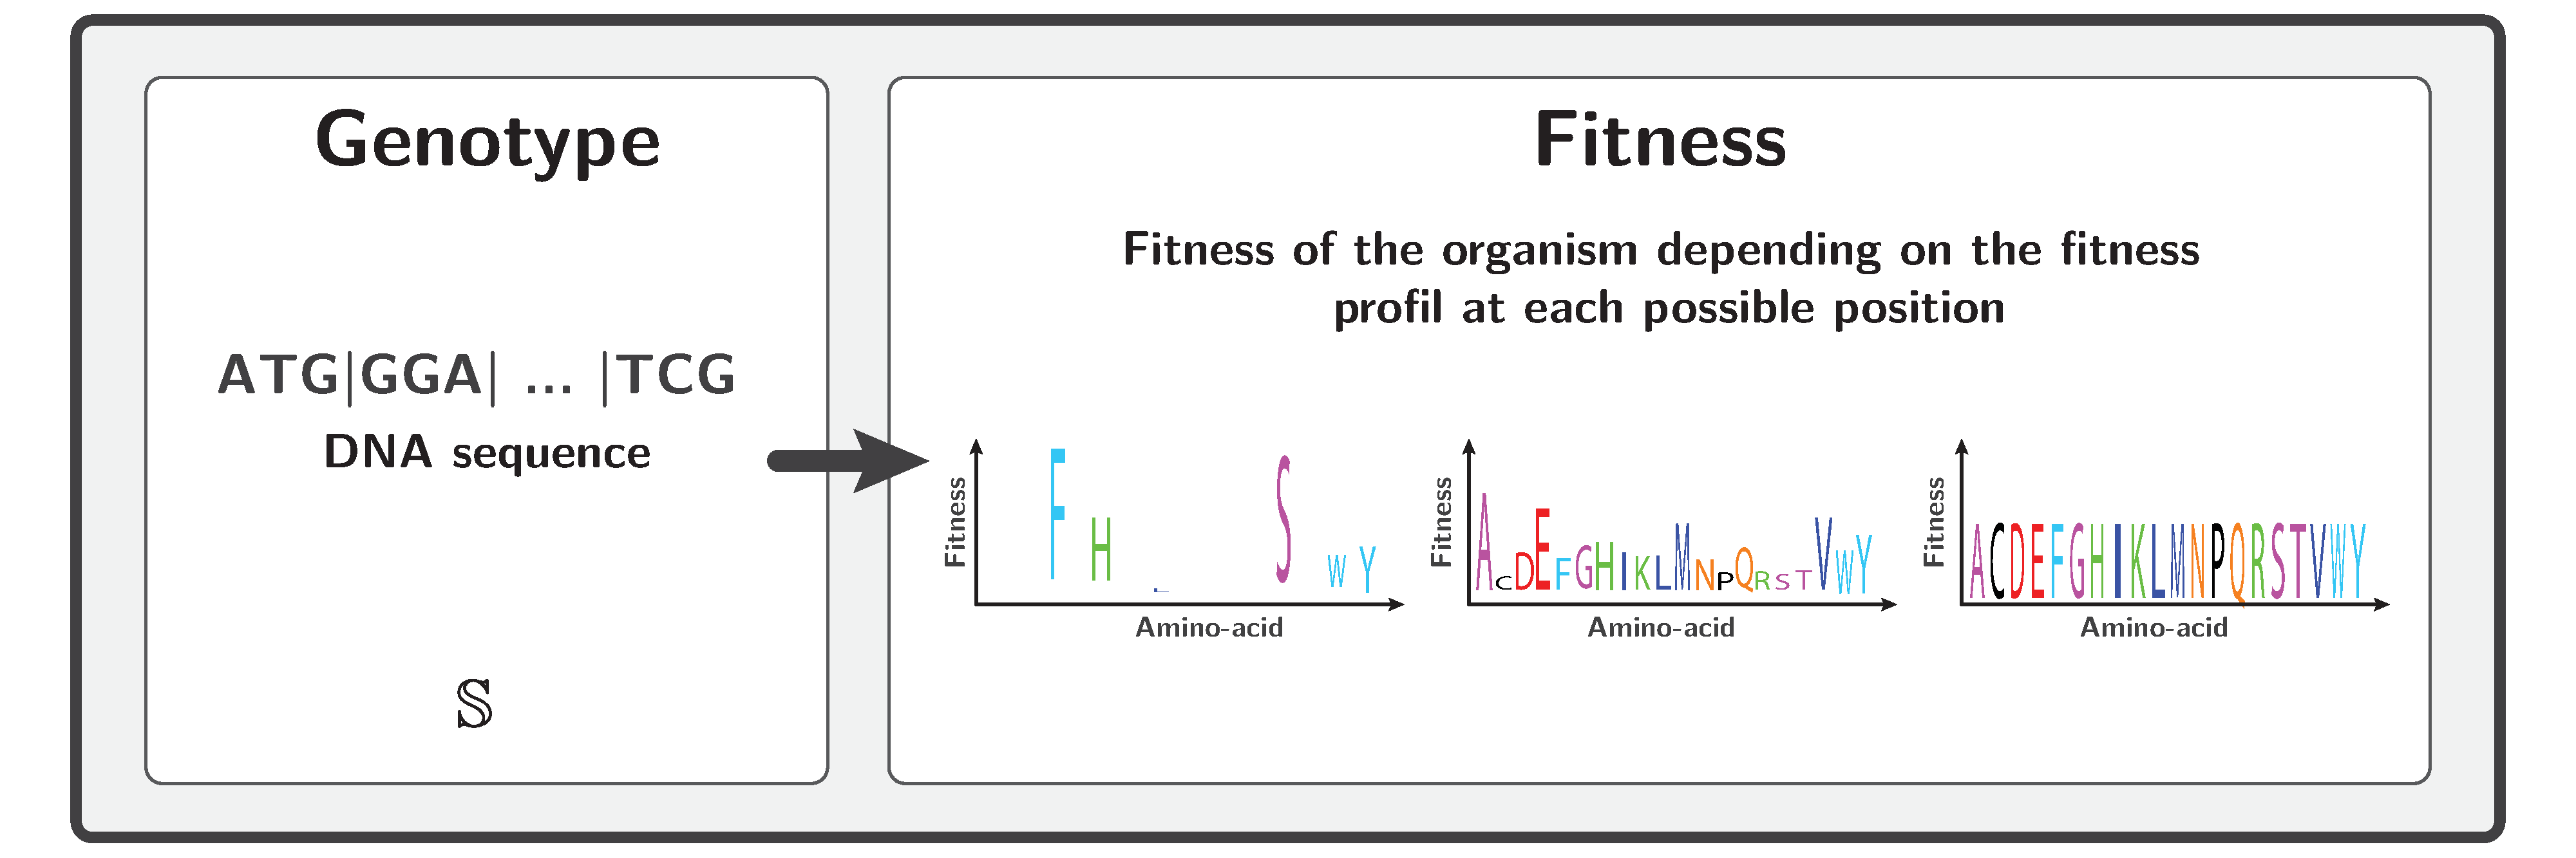
\includegraphics[width=\textwidth] {ModelSimuDiv}
\end{center}

The next change in the protein coding \acrshort{DNA} and the time to next the event is chosen using Gillespie algorithm, according to the rates of \gls{substitution} between \glspl{codon}:
\begin{equation}
{\submatrix_{\itoj}}
    = \mu_{\itoj} \dfrac{4 \Ne s \left( \mathbb{S}^{t},\mathbb{S}^{t+1}\right)}{{1 - \e^{-4 \Ne s \left( \mathbb{S}^{t},\mathbb{S}^{t+1}\right)} }},
\end{equation}
where ${\submatrix_{\itoj}} = \mu_{\itoj}$ in the case of \glspl{synonymous}.


\begin{figure}[H]
    \centering
    \begin{minipage}{0.32\linewidth}
        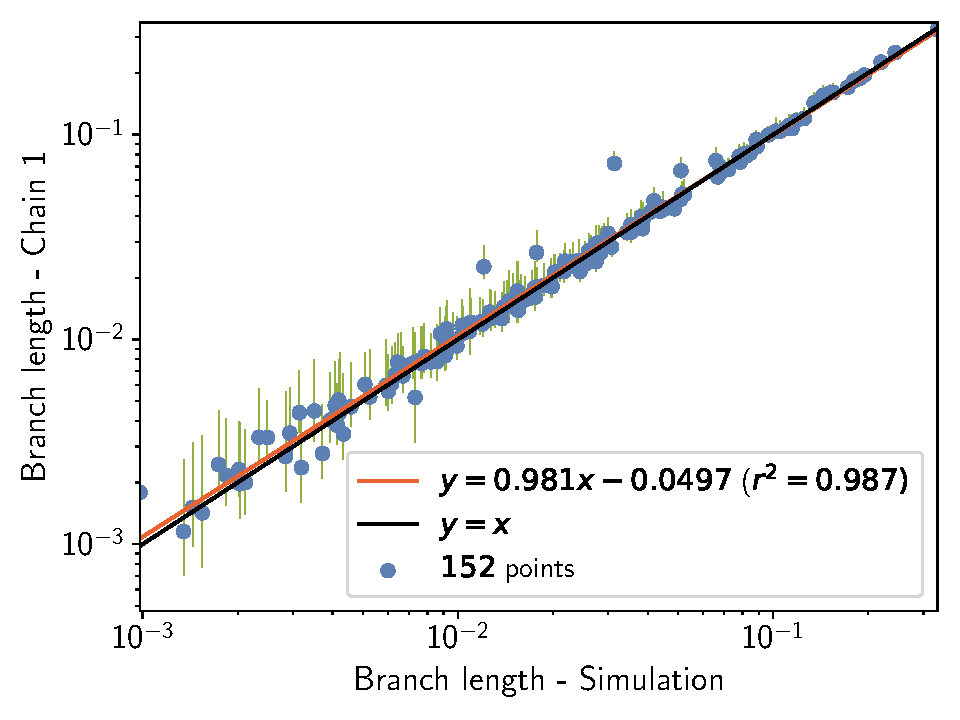
\includegraphics[width=\linewidth, page=1]{simulations/BranchWise_SimuDiv_SiteMutSelBranchNe_BranchCorrelation_Log10BranchLength}
    \end{minipage} \hfill
    \begin{minipage}{0.32\linewidth}
        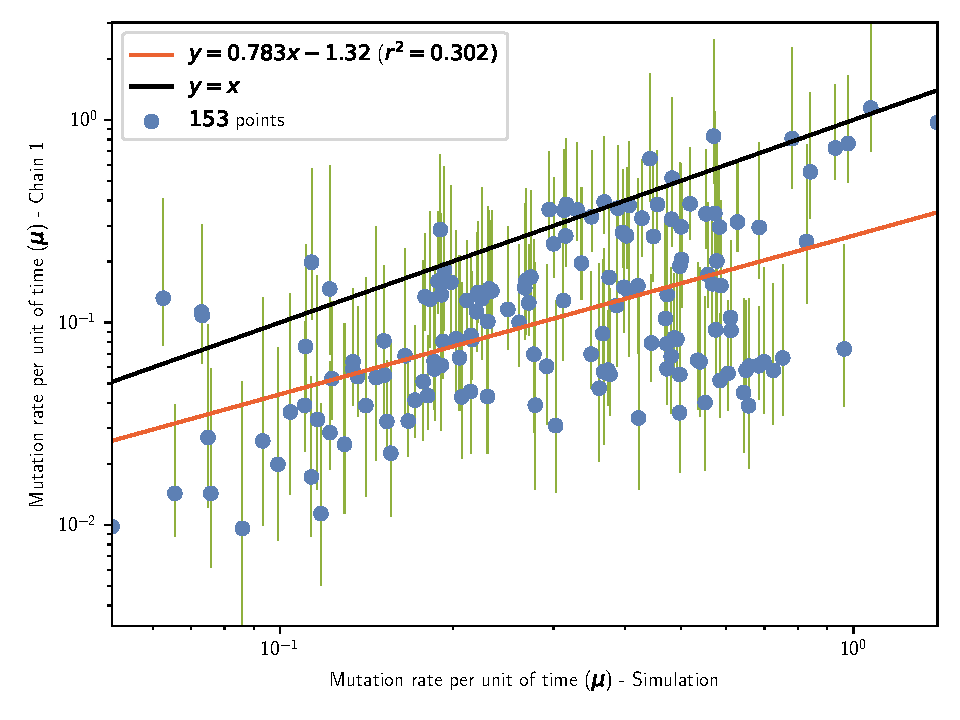
\includegraphics[width=\linewidth, page=1]{simulations/BranchWise_SimuDiv_SiteMutSelBranchNe_BranchCorrelation_LogMutationRatePerTime}
    \end{minipage} \hfill
    \begin{minipage}{0.32\linewidth}
        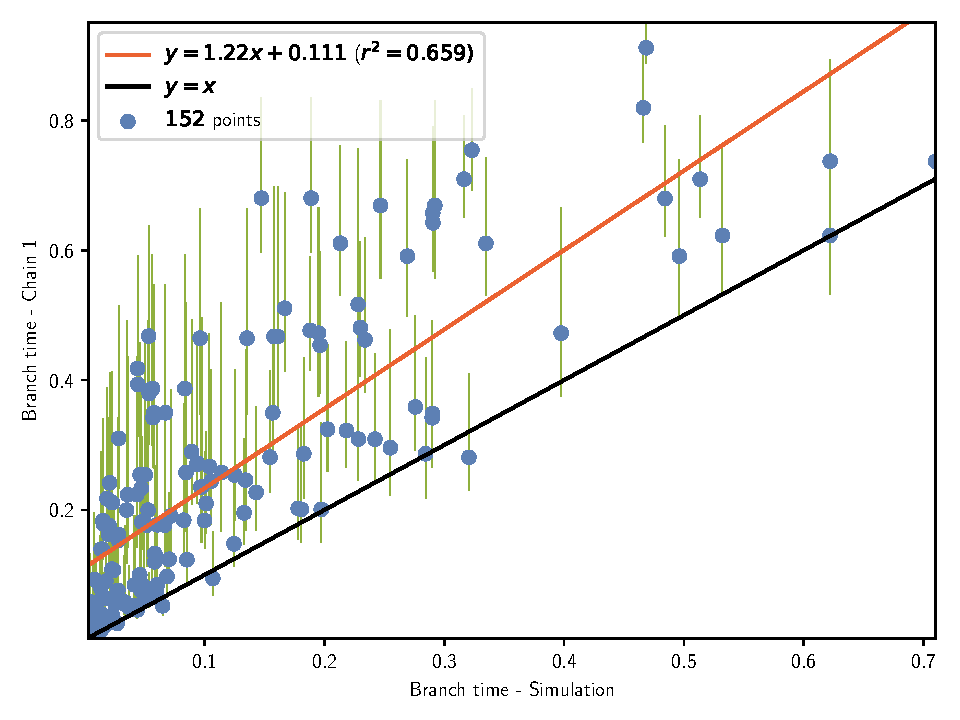
\includegraphics[width=\linewidth, page=1]{simulations/BranchWise_SimuDiv_SiteMutSelBranchNe_BranchCorrelation_BranchTime}
    \end{minipage} \hfill
    \begin{minipage}{0.32\linewidth}
        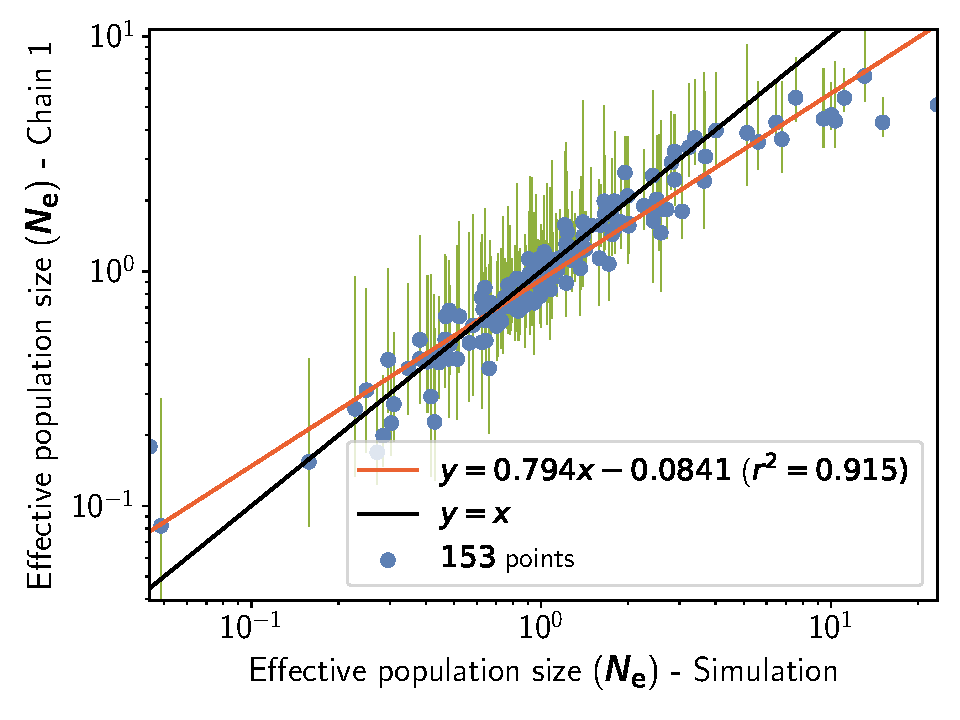
\includegraphics[width=\linewidth, page=1]{simulations/BranchWise_SimuDiv_SiteMutSelBranchNe_BranchCorrelation_LogPopulationSize}
    \end{minipage}
    \begin{minipage}{0.32\linewidth}
        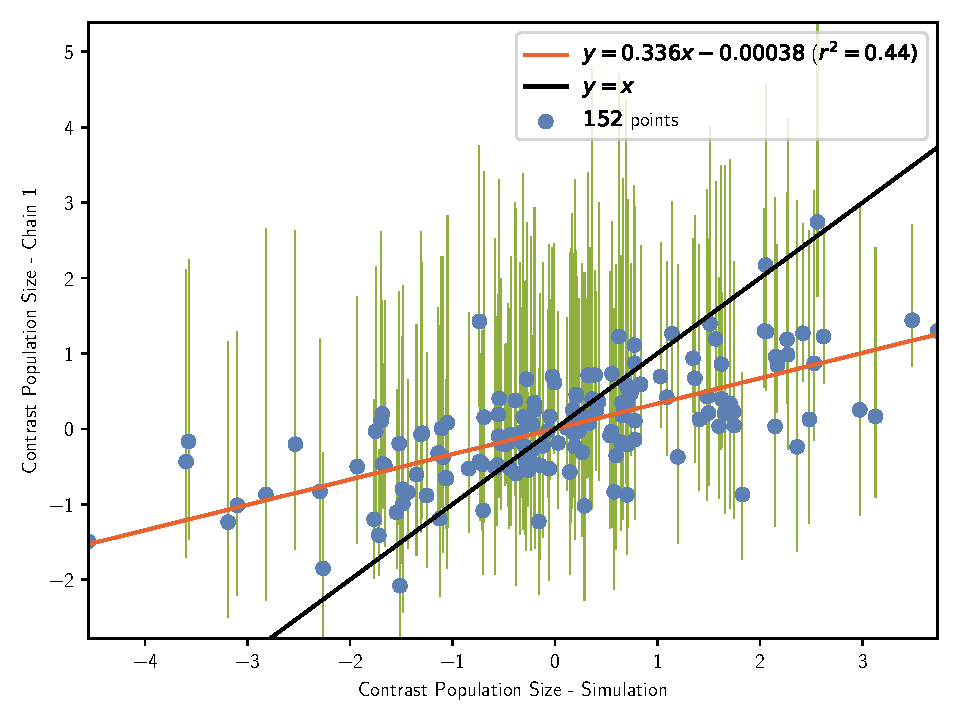
\includegraphics[width=\linewidth, page=1]{simulations/BranchWise_SimuDiv_SiteMutSelBranchNe_BranchCorrelation_ContrastPopulationSize}
    \end{minipage} \hfill
    \caption[Inferred branch parameters for SimuDiv]{
    Inferred branch parameters under simulation accounting for long term fluctuation of $\Ne$, mutation rate per generation and generation time.
    }
\end{figure}


\begin{figure}[H]
    \centering
    \begin{minipage}{0.49\linewidth}
        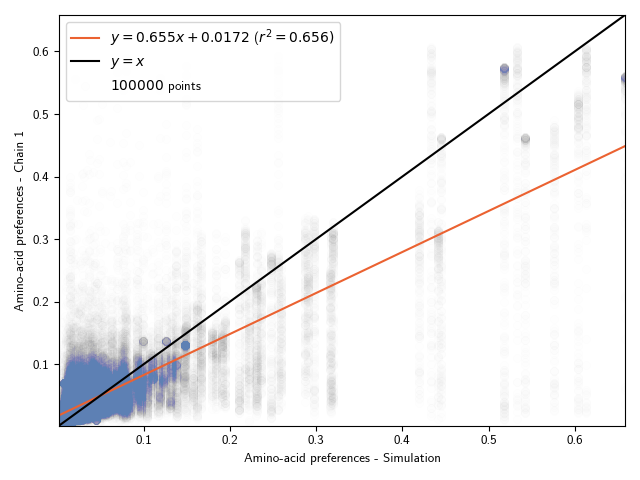
\includegraphics[width=\linewidth, page=1]{simulations/BranchWise_SimuDiv_SiteMutSelBranchNe_ProfileCorrelation.png}
    \end{minipage} \hfill
    \begin{minipage}{0.49\linewidth}
        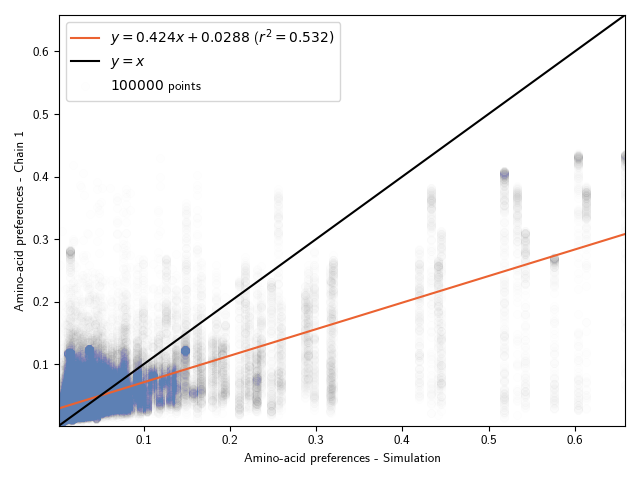
\includegraphics[width=\linewidth, page=1]{simulations/BranchWise_SimuDiv_SiteMutSel_ProfileCorrelation.png}
    \end{minipage}
    \caption[Inferred site amino-acid profiles for SimuDiv]{
    Inferred and simulated site specific amino-acid profiles under simulation accounting for long term fluctuation of $\Ne$, mutation rate per generation and generation time.
    Estimation with fluctuating branch $\Ne$ (left panel) or constant $\Ne$ (right panel).}
\end{figure}

\begin{table}[H]
    \centering
    \noindent\adjustbox{max width=\textwidth}{%
    \begin{tabu}{|c|c|c|}
        \hline
        \textbf{Experiment} & $\langle \entropy \rangle$ (\textbf{branch} $\Ne$) & $\langle \entropy \rangle$ (\textbf{constant} $\Ne$) \\ \hline
        \hline
        SimuDiv, chain 1 & $2.30 \pm 0.04$ & $2.45 \pm 0.02$\\ \hline
        SimuDiv, chain 2 & $2.30 \pm 0.04$ & $2.45 \pm 0.02$\\ \hline
    \end{tabu}}
    \caption[Inferred amino-acids entropy for SimuDiv]{
    Estimated amino-acids entropy.
    Simulation accounting for long term fluctuation of $\Ne$, mutation rate per generation and generation time.
    Estimated with the inference model of site selection for amino-acid, and branch fluctuation of $\Ne$ (left column), or under the assumption of constant $\Ne$ (right column)}
\end{table}

\subsection{Wright-Fisher with polymorphism}

The evolutionary dynamics was formalized as a Wright-Fisher model with mutation, selection and drift. The population is assumed to be panmictic, with with \gls{effective-population-size} $\Ne$ and with non-overlapping generations.

\begin{center}
    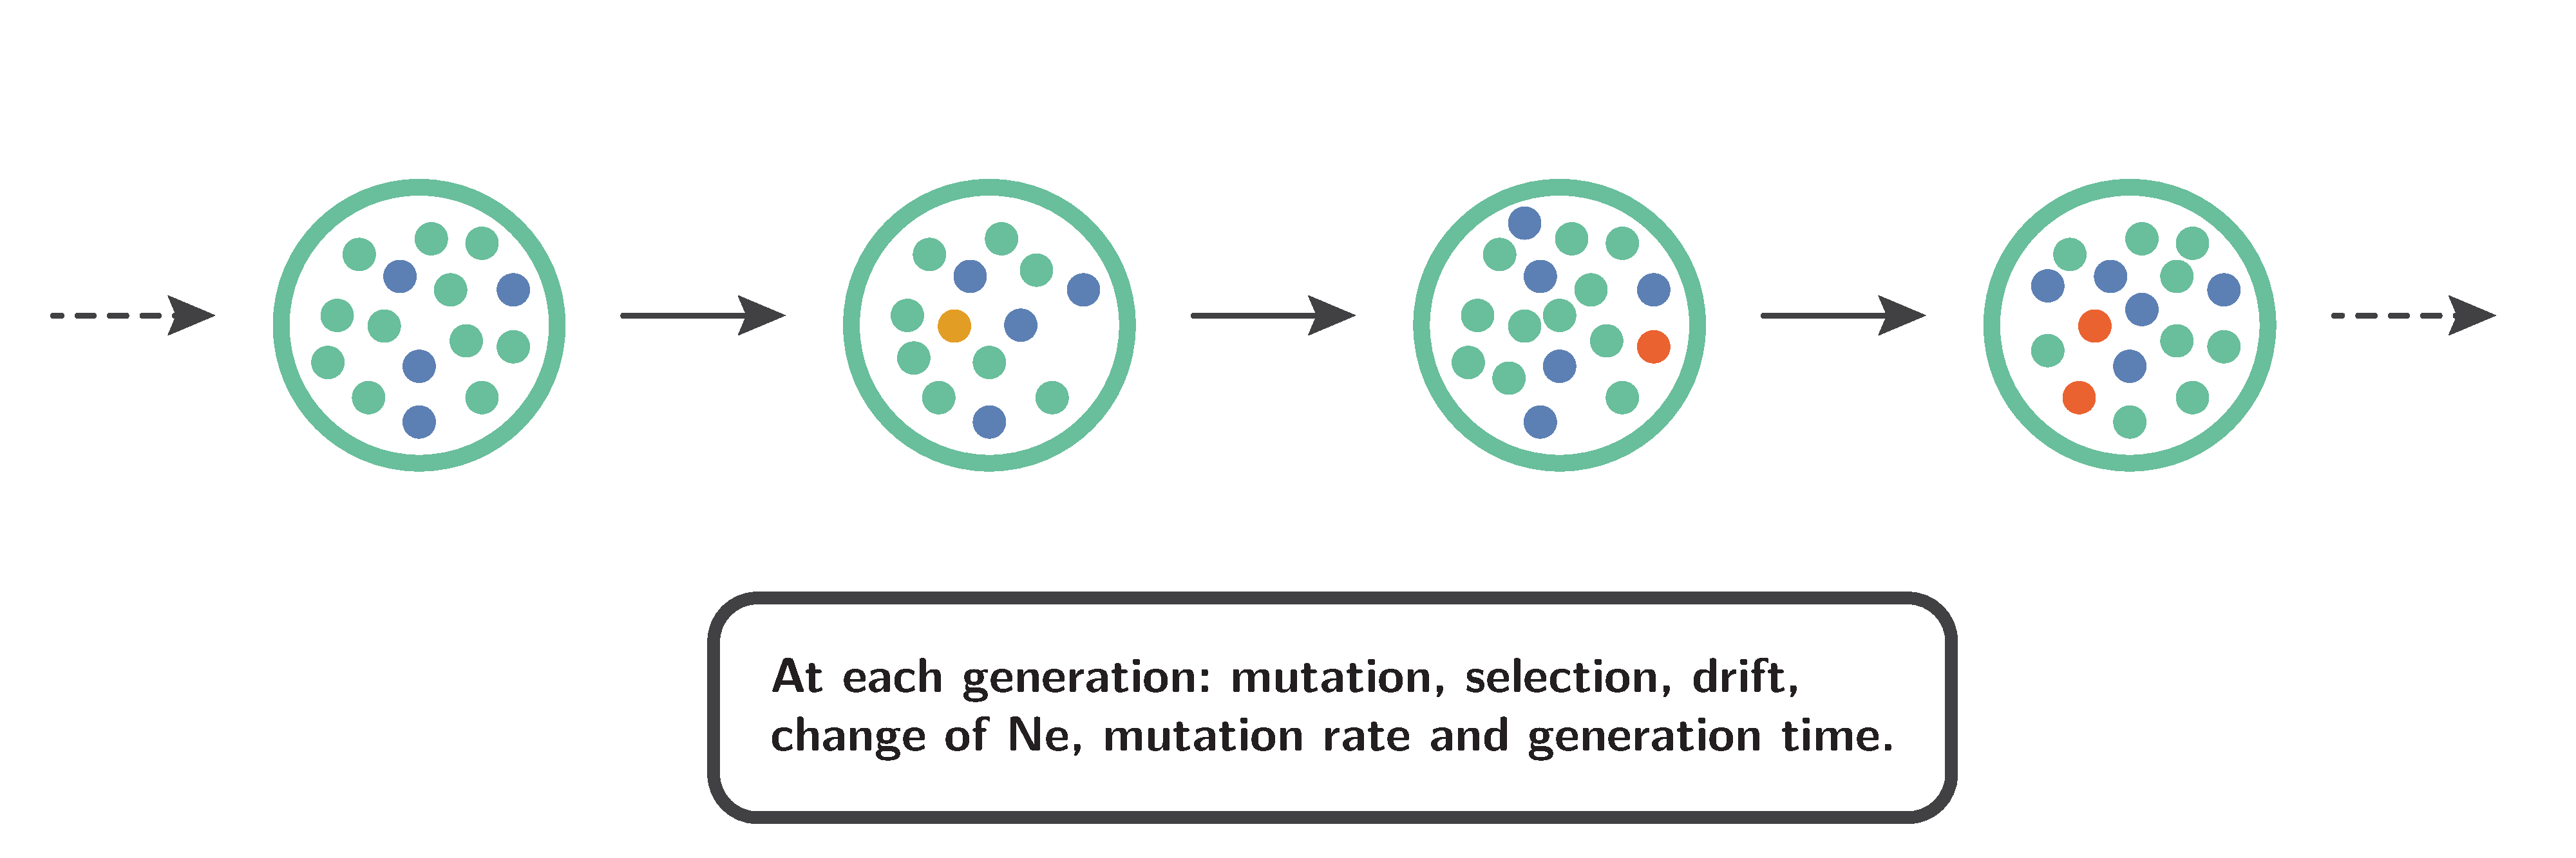
\includegraphics[width=\textwidth] {ModelSimuPoly}
\end{center}

\begin{figure}[H]
    \centering
    \begin{minipage}{0.32\linewidth}
        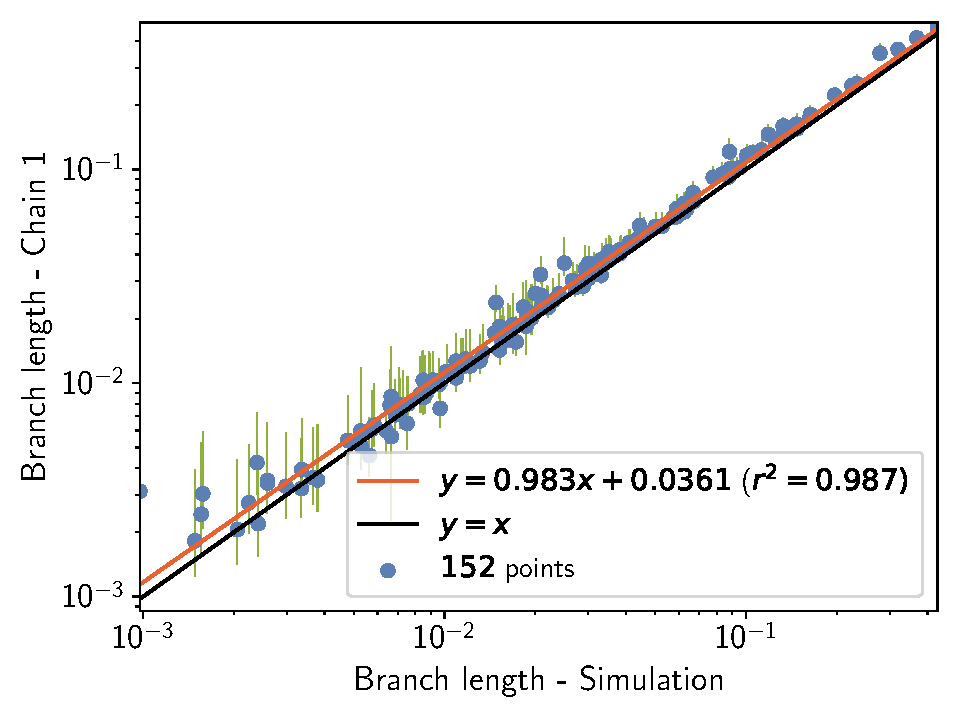
\includegraphics[width=\linewidth, page=1]{simulations/SimuPoly_SiteMutSelBranchNe_BranchCorrelation_Log10BranchLength}
    \end{minipage} \hfill
    \begin{minipage}{0.32\linewidth}
        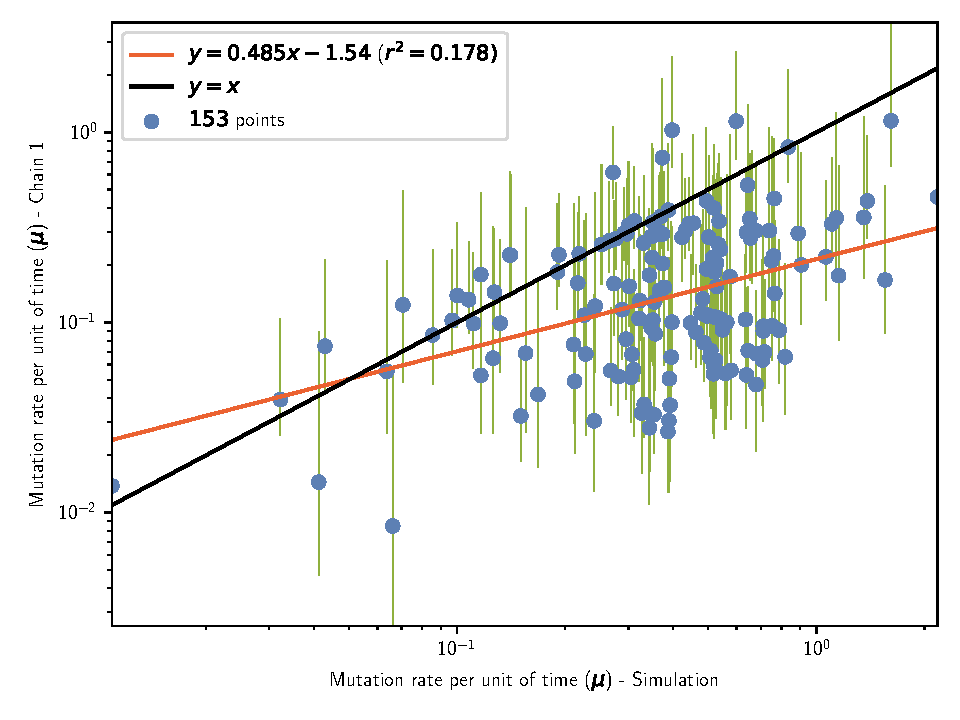
\includegraphics[width=\linewidth, page=1]{simulations/SimuPoly_SiteMutSelBranchNe_BranchCorrelation_LogMutationRatePerTime}
    \end{minipage} \hfill
    \begin{minipage}{0.32\linewidth}
        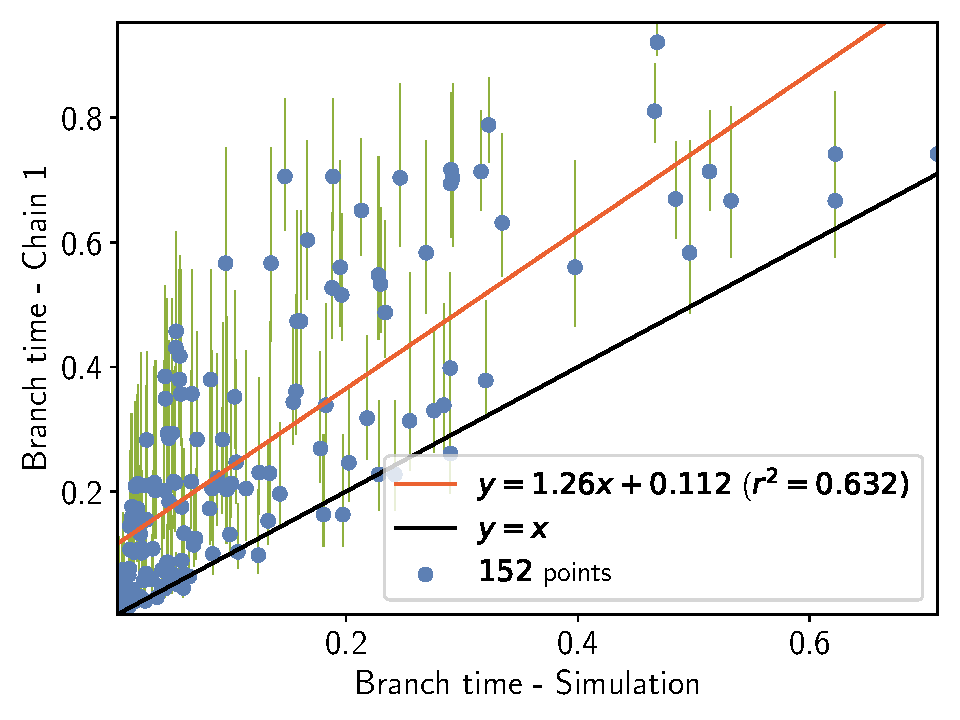
\includegraphics[width=\linewidth, page=1]{simulations/SimuPoly_SiteMutSelBranchNe_BranchCorrelation_BranchTime}
    \end{minipage} \hfill
    \begin{minipage}{0.32\linewidth}
        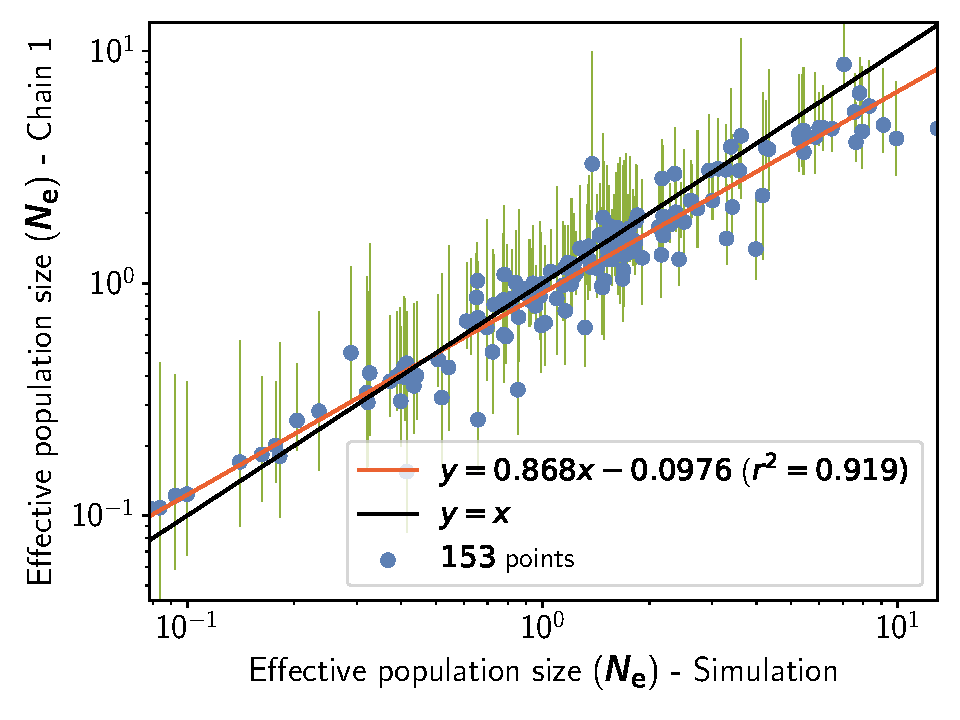
\includegraphics[width=\linewidth, page=1]{simulations/SimuPoly_SiteMutSelBranchNe_BranchCorrelation_LogPopulationSize}
    \end{minipage}
    \begin{minipage}{0.32\linewidth}
        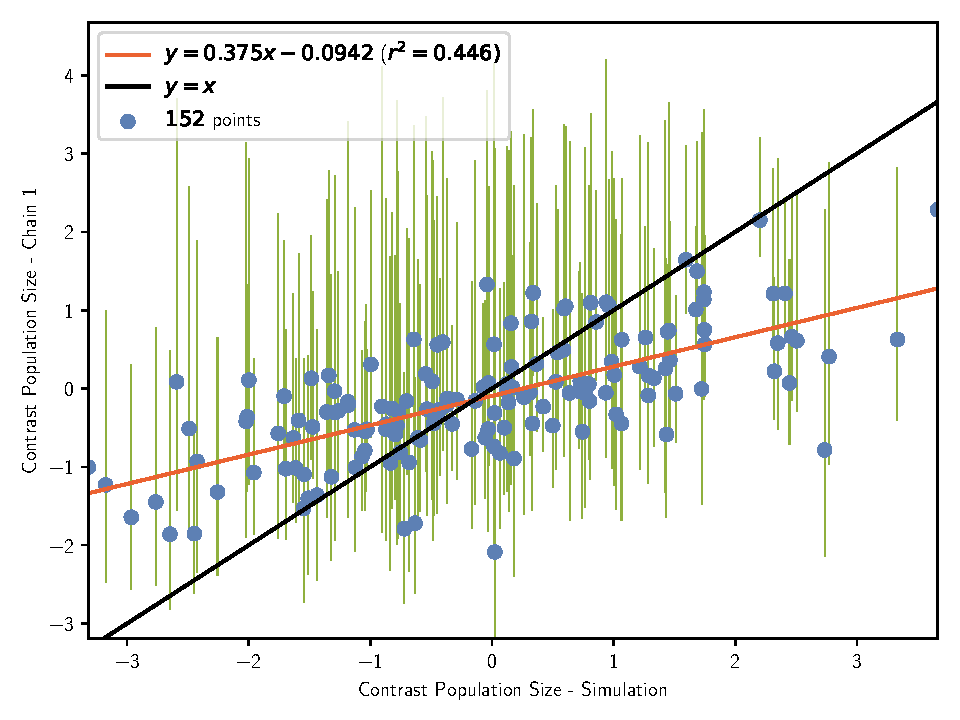
\includegraphics[width=\linewidth, page=1]{simulations/SimuPoly_SiteMutSelBranchNe_BranchCorrelation_ContrastPopulationSize}
    \end{minipage} \hfill
    \caption[Inferred branch parameters for SimuPoly]{
    Inferred branch parameters under simulation accounting for finite population effects, site linkage and short term fluctuation of $\Ne$.
    }
\end{figure}


\begin{figure}[H]
    \centering
    \begin{minipage}{0.49\linewidth}
        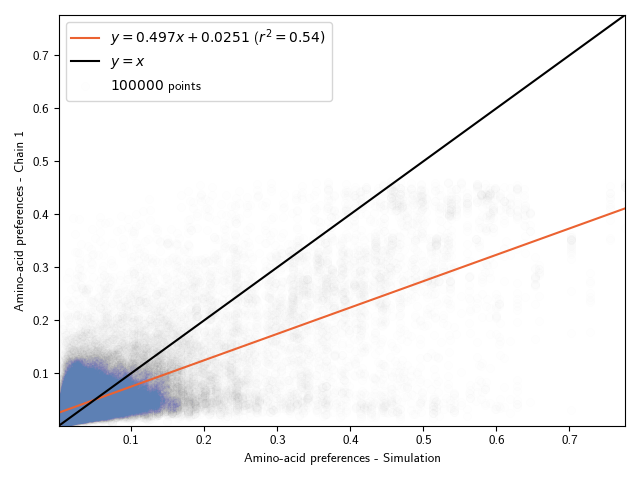
\includegraphics[width=\linewidth, page=1]{simulations/SimuPoly_SiteMutSelBranchNe_ProfileCorrelation.png}
    \end{minipage} \hfill
    \begin{minipage}{0.49\linewidth}
        \includegraphics[width=\linewidth, page=1]{simulations/SimuPoly_SiteMutSel_ProfileCorrelation.png}
    \end{minipage}
    \caption[Inferred site amino-acid profiles for SimuPoly]{
    Inferred and simulated site specific amino-acid profiles under simulation accounting for finite population effects, site linkage and short term fluctuation of $\Ne$.
    Estimation with fluctuating branch $\Ne$ (left panel) or constant $\Ne$ (right panel).}
\end{figure}

\begin{table}[H]
    \centering
    \noindent\adjustbox{max width=\textwidth}{%
    \begin{tabu}{|c|c|c|}
        \hline
        \textbf{Experiment} & $\langle \entropy \rangle$ (\textbf{branch} $\Ne$) & $\langle \entropy \rangle$ (\textbf{constant} $\Ne$) \\ \hline
        \hline
        SimuPoly, chain 1 & $2.47 \pm 0.03$ & $2.37 \pm 0.02$\\ \hline
        SimuPoly, chain 2 & $2.47 \pm 0.03$ & $2.37 \pm 0.02$\\ \hline
    \end{tabu}}
    \caption[Inferred amino-acid entropy for SimuPoly]{
    Estimated amino-acids entropy under simulation accounting for finite population effects, site linkage and short term fluctuation of $\Ne$.
    Obtained with the inference model of site selection for amino-acid, and branch fluctuation of $\Ne$ (left column), or under the assumption of constant $\Ne$ (right column)}
\end{table}

\subsection{Fisher geometric landscape}

We simulated \glspl{substitution} in a protein using an adaptation of Fisher's geometric landscape.
In the original context, the \gls{Phenotype} is a vector ($\phenoGeo$) in a multidimensional space, where the number of dimensions is often termed complexity.
From a \gls{Phenotype}, the fitness is a monotonously decreasing function of the \gls{Phenotype} distance to $0$.
The exact functional phenotype-fitness map depend on $2$ external parameters controlling for strength ($\alpha$) and epistasis ($\beta$).
If the phenotype-fitness map is explicit, the genotype-phenotype map is more pervasive.
Mutations are seen has displacement of the \gls{Phenotype} in the multidimensional space.
Beneficial mutations are moving the \gls{Phenotype} closer to $0$, whereas deleterious mutations are moving the \gls{Phenotype} further away.
In such original context, the distribution of mutational effects is not dependent on the current genotype, but this can be relaxed using a genotype-phenotype map.\\

In a protein context, the genotype-phenotype map can be defined by assigning to each of the $20$ amino-acid a vector in the multidimensional space.
Since different sites of the protein do not have the same physico-chimical properties, we can define a specific genotype-phenotype map for each position of the sequence.
Overall, the protein \gls{Phenotype} is computed as the sum of site-specific multidimensional vectors, obtained by accessing the amino-acid present at each site of the protein.
From a \acrshort{DNA} sequence $\mathbb{S}^t$ after $t$ \glspl{substitution}, the protein's \gls{Phenotype} is given by:
\begin{equation}
    \phenoGeo\left(\mathbb{S}^{t}\right) = \sum\limits_{1 \leq \site \leq \Nsite} \phenoGeo_{\site} \left(\mathbb{S}^t(\site) \right),
\end{equation}
where $\phenoGeo_{\site}$ is the genotype-phenotype map at site $\site$.\\

And the Wrightian fitness of $\mathbb{S}^t$ is :
\begin{equation}
    w\left( \phenoGeo\left(\mathbb{S}^{t}\right) \right) = e^{-\alpha \left| \phenoGeo\left(\mathbb{S}^{t}\right) \right|^{\beta}},
\end{equation}
where strength ($\alpha > 0$) and epistasis ($\beta$) are parameters of the fitness function.
\begin{center}
    \includegraphics[width=\textwidth] {ModelSimuGeo}
\end{center}
For each possible mutant ($t+1$ substitutions), we compute $\phenoGeo\left(\mathbb{S}^{t+1}\right)$ from the updated sequence $\mathbb{S}^{t+1}$, and subsequently the selection coefficient of the mutant:
\begin{equation}
    s \left( \mathbb{S}^{t},\mathbb{S}^{t+1}\right) = \dfrac{ w\left( \phenoGeo\left(\mathbb{S}^{t+1}\right) \right) - w\left( \phenoGeo\left(\mathbb{S}^{t}\right) \right)}{w\left( \phenoGeo\left(\mathbb{S}^{t}\right) \right)}.
\end{equation}
The next change in the protein coding \acrshort{DNA} and the time to next the event is chosen using Gillespie algorithm, according to the rates of \gls{substitution} between \glspl{codon}:
\begin{equation}
{\submatrix_{\itoj}}
    = \mu_{\itoj} \dfrac{4 \Ne s \left( \mathbb{S}^{t},\mathbb{S}^{t+1}\right)}{{1 - \e^{-4 \Ne s \left( \mathbb{S}^{t},\mathbb{S}^{t+1}\right)} }},
\end{equation}
where ${\submatrix_{\itoj}} = \mu_{\itoj}$ in the case of \glspl{synonymous}.

\begin{figure}[H]
    \centering
    \begin{minipage}{0.32\linewidth}
        \includegraphics[width=\linewidth, page=1]{simulations/SimuGeo_SiteMutSelBranchNe_BranchCorrelation_Log10BranchLength}
    \end{minipage} \hfill
    \begin{minipage}{0.32\linewidth}
        \includegraphics[width=\linewidth, page=1]{simulations/SimuGeo_SiteMutSelBranchNe_BranchCorrelation_LogMutationRatePerTime}
    \end{minipage} \hfill
    \begin{minipage}{0.32\linewidth}
        \includegraphics[width=\linewidth, page=1]{simulations/SimuGeo_SiteMutSelBranchNe_BranchCorrelation_BranchTime}
    \end{minipage} \hfill
    \begin{minipage}{0.32\linewidth}
        \includegraphics[width=\linewidth, page=1]{simulations/SimuGeo_SiteMutSelBranchNe_BranchCorrelation_LogPopulationSize}
    \end{minipage}
    \begin{minipage}{0.32\linewidth}
        \includegraphics[width=\linewidth, page=1]{simulations/SimuGeo_SiteMutSelBranchNe_BranchCorrelation_ContrastPopulationSize}
    \end{minipage} \hfill
    \caption[Inferred branch parameters for SimuGeo]{
    Inferred branch parameters under simulation accounting for site epistasis (Geometric landscape), thus fluctuation of the selection coefficient along the phylogeny.
    }
\end{figure}


\begin{table}[H]
    \centering
    \noindent\adjustbox{max width=\textwidth}{%
    \begin{tabu}{|c|c|c|}
        \hline
        \textbf{Experiment} & $\langle \entropy \rangle$ (\textbf{branch} $\Ne$) & $\langle \entropy \rangle$ (\textbf{constant} $\Ne$) \\ \hline
        \hline
        SimuGeo, chain 1 & $2.27 \pm 0.02$ & $2.46 \pm 0.02$\\ \hline
        SimuGeo, chain 2 & $2.23 \pm 0.04$ & $2.46 \pm 0.02$\\ \hline
    \end{tabu}}
    \caption[Entropy of amino-acids for SimuGeo]{
    Estimated amino-acids entropy under under simulation accounting for site epistasis (Geometric landscape), thus fluctuation of the selection coefficient along the phylogeny.
    Obtained with the inference model of site selection for amino-acid, and branch fluctuation of $\Ne$ (left column), or under the assumption of constant $\Ne$ (right column)}
\end{table}

\subsection{Protein folding probability}
We simulated \glspl{substitution} in the protein phosphatase ($\Nsite=300$ \gls{codon} sites) as in Goldstein \& Pollock (2017).
From a \acrshort{DNA} sequence $\mathbb{S}^t$ after $t$ \glspl{substitution}, we compute the free energy of the folded state $\Base_{\mathrm{F}}\left(\mathbb{S}^{t}\right)$, using the $3$-dimensional structure of the folded state and pair-wise contact energies between neighboring amino-acid residues:
\begin{equation}
    G_{\mathrm{F}}\left(\mathbb{S}^{t}\right) = \sum\limits_{1 \leq \site \leq \Nsite} \sum\limits_{r \in \mathcal{N}(\site)} I \left(\mathbb{S}^t(\site), \mathbb{S}^t(r) \right),
\end{equation}
where $I(a,b)$ is the pair-wise contact energies between amino-acid $a$ and $b$, using contact potentials estimated by Miya-zawa and Jernigan, and $\mathcal{N}(\site)$ are the neighbor residues of site $\site$ (closer than $7\angstrom$) in the $3$D structure.\\

The free energy of unfolded states $G_{\mathrm{U}}\left(\mathbb{S}^{t}\right)$ is approximated using $55$ decoy $3$D structures that supposedly represent a sample of possible unfolded states:
\begin{equation}
    G_{\mathrm{U}}\left(\mathbb{S}^{t}\right) = \langle G\left(\mathbb{S}^{t}\right) \rangle - kT \ln (1.0\mathrm{E}^{160}) - \dfrac{2 \left[ \langle G\left(\mathbb{S}^{t}\right)^2 \rangle - \langle G\left(\mathbb{S}^{t}\right) \rangle^2\right] }{kT}
\end{equation}
where the average $\langle . \rangle$ runs other the $55$ decoy $3$D structures, and $k$ is the Boltzmann constant and $T$ the temperature in Kelvin.\\

From the energy of folded and unfolded states, we can compute the difference in free energy between the states:
\begin{equation}
    \phenoFold\left(\mathbb{S}^{t}\right) = G_{\mathrm{F}}\left(\mathbb{S}^{t}\right) - G_{\mathrm{U}}\left(\mathbb{S}^{t}\right)
\end{equation}

Wrightian fitness is defined as the probability of our protein to be in the folded state:
\begin{equation}
    w(\phenoFold\left(\mathbb{S}^{t}\right)) = \dfrac{P_{\mathrm{F}}\left(\mathbb{S}^{t}\right)}{P_{\mathrm{F}}\left(\mathbb{S}^{t}\right) + P_{\mathrm{U}}\left(\mathbb{S}^{t}\right)} = \dfrac{e^{-\beta G_{\mathrm{F}}\left(\mathbb{S}^{t}\right) }}{e^{-\beta G_{\mathrm{F}} \left(\mathbb{S}^{t}\right) } + e^{-\beta G_{\mathrm{U}}\left(\mathbb{S}^{t}\right) }} = \dfrac{1}{1 + e^{\beta \phenoFold\left(\mathbb{S}^{t}\right) }},
\end{equation}
where $\beta$ is the inverse of the temperature ($\beta=1/kT$).
\begin{center}
    \includegraphics[width=\textwidth] {ModelSimuFold}
\end{center}
For each possible mutant ($t+1$ substitutions), we compute $\phenoFold^{t+1}$ from the updated sequence $\mathbb{S}^{t+1}$, and subsequently the selection coefficient of the mutant:
\begin{equation}
    s \left( \mathbb{S}^{t},\mathbb{S}^{t+1}\right) = \dfrac{ w\left( \phenoFold\left(\mathbb{S}^{t+1}\right) \right) - w\left( \phenoFold\left(\mathbb{S}^{t}\right) \right)}{w\left( \phenoFold\left(\mathbb{S}^{t}\right) \right)}.
\end{equation}
The next change in the protein coding \acrshort{DNA} and the time to next the event is chosen using Gillespie algorithm, according to the rates of \gls{substitution} between \glspl{codon}:
\begin{equation}
{\submatrix_{\itoj}}
    = \mu_{\itoj} \dfrac{4 \Ne s \left( \mathbb{S}^{t},\mathbb{S}^{t+1}\right)}{{1 - \e^{-4 \Ne s \left( \mathbb{S}^{t},\mathbb{S}^{t+1}\right)} }},
\end{equation}
where ${\submatrix_{\itoj}} = \mu_{\itoj}$ in the case of \glspl{synonymous}.

\begin{figure}[H]
    \centering
    \begin{minipage}{0.32\linewidth}
        \includegraphics[width=\linewidth, page=1]{simulations/SimuFold_SiteMutSelBranchNe_BranchCorrelation_Log10BranchLength}
    \end{minipage} \hfill
    \begin{minipage}{0.32\linewidth}
        \includegraphics[width=\linewidth, page=1]{simulations/SimuFold_SiteMutSelBranchNe_BranchCorrelation_LogMutationRatePerTime}
    \end{minipage} \hfill
    \begin{minipage}{0.32\linewidth}
        \includegraphics[width=\linewidth, page=1]{simulations/SimuFold_SiteMutSelBranchNe_BranchCorrelation_BranchTime}
    \end{minipage} \hfill
    \begin{minipage}{0.32\linewidth}
        \includegraphics[width=\linewidth, page=1]{simulations/SimuFold_SiteMutSelBranchNe_BranchCorrelation_LogPopulationSize}
    \end{minipage}
    \begin{minipage}{0.32\linewidth}
        \includegraphics[width=\linewidth, page=1]{simulations/SimuFold_SiteMutSelBranchNe_BranchCorrelation_ContrastPopulationSize}
    \end{minipage} \hfill
    \caption[Inferred branch parameters for SimuFold]{
    Inferred branch parameters under simulation accounting for site epistasis (folding stability model), thus fluctuation of the selection coefficient along the phylogeny.
    }
\end{figure}

\begin{table}[H]
    \centering
    \noindent\adjustbox{max width=\textwidth}{%
    \begin{tabu}{|c|c|c|}
        \hline
        \textbf{Experiment} & $\langle \entropy \rangle$ (\textbf{branch} $\Ne$) & $\langle \entropy \rangle$ (\textbf{constant} $\Ne$) \\ \hline
        \hline
        SimuFold, chain 1 & $1.31 \pm 0.05$ & $1.61 \pm 0.03$\\ \hline
        SimuFold, chain 2 & $1.30 \pm 0.04$ & $1.60 \pm 0.03$\\ \hline
    \end{tabu}}
    \caption[Entropy of amino-acids in SimuFold]{
    Estimated amino-acids entropy under simulation accounting for site epistasis (folding stability model), thus fluctuation of the selection coefficient along the phylogeny.
    Obtained with the inference model of site selection for amino-acid, and branch fluctuation of $\Ne$ (left column), or under the assumption of constant $\Ne$ (right column)}
\end{table}


\section{Empirical data in mammals}

\subsection{Chain convergence}
Obtained with the inference model of site selection for amino-acid, and branch fluctuation of $\Ne$.

\begin{figure}[H]
    \centering
    \begin{minipage}{0.49\linewidth}
        \includegraphics[width=\linewidth, page=1]{mammals/18CDS_SiteMutSelBranchNe_R1_ProfileCorrelation.png}
    \end{minipage} \hfill
    \begin{minipage}{0.49\linewidth}
        \includegraphics[width=\linewidth, page=1]{mammals/18CDS_SiteMutSelBranchNe_R1_LogPopulationSizeCorrelation}
    \end{minipage}
    \caption[Chain convergence of site profiles and branche $\Ne$]{
    Chain convergence of site amino-acid preferences (left panel) and branch $\Ne$ (right panel).}
\end{figure}

\subsection{Traits estimation \& correlation (replicate 1, chain 1)}
Obtained with the inference model of site selection for amino-acid, and branch fluctuation of $\Ne$.

\begin{table}[H]
    \centering
\noindent\adjustbox{max width=\textwidth}{%
\begin{tabu}{|c||c|c|c|c|c|}
\hline
\textbf{Covariance ($\bm{\Sigma}$)} & $\bm{N_{\text{e}}}$ & $\bm{\mu}$ & \textbf{Maximum longevity } & \textbf{Adult weight } & \textbf{Female maturity }\\
\hhline{|=#=|=|=|=|=|}
$\bm{N_{\text{e}}}$ & $0.281^{**}$ & $0.324^{**}$ & $-0.268^{**}$ & $-1.29^{**}$ & $-0.308^{**}$\\\hline
$\bm{\mu}$ & - & $1.93^{**}$ & $-1.12^{**}$ & $-5.19^{**}$ & $-1.43^{**}$\\\hline
\textbf{Maximum longevity } & - & - & $0.934^{**}$ & $3.58^{**}$ & $1.01^{**}$\\\hline
\textbf{Adult weight } & - & - & - & $19.9^{**}$ & $4.48^{**}$\\\hline
\textbf{Female maturity } & - & - & - & - & $1.53^{**}$\\\hline
\end{tabu}}

    \caption[Covariance matrix in mammals]{
    Covariance coefficient between effective population size~($\Ne$), mutation rate per site per unit of time~($\mu$), and life-history traits (Maximum longevity, adult weight and female maturity) were computed in placental mammals.
    Asterisks indicate strength of support ($\smash{^{*}} pp > 0.95$, $\smash{^{**}} pp > 0.975$).}
\end{table}

\begin{table}[H]
    \centering
\noindent\adjustbox{max width=\textwidth}{%
\begin{tabu}{|c||c|c|c|c|c|}
\hline
\textbf{Partial coefficient} & $\bm{N_{\mathrm{e}}}$ & $\bm{\mu}$ & \textbf{Maximum longevity } & \textbf{Adult weight } & \textbf{Female maturity }\\
\hhline{|=#=|=|=|=|=|}
$\bm{N_{\mathrm{e}}}$ & - & $-0.146$ & $-0.177$ & $-0.265^{*}$ & $-0.0223$\\\hline
$\bm{\mu}$ & - & - & $-0.283^{*}$ & $-0.396^{**}$ & $-0.327^{**}$\\\hline
\textbf{Maximum longevity } & - & - & - & $0.236^{*}$ & $0.383^{**}$\\\hline
\textbf{Adult weight } & - & - & - & - & $0.179$\\\hline
\textbf{Female maturity } & - & - & - & - & -\\\hline
\end{tabu}}

    \caption[Partial correlation coefficient matrix in mammals]{
    Partial correlation coefficient between effective population size~($\Ne$), mutation rate per site per unit of time~($\mu$), and life-history traits (Maximum longevity, adult weight and female maturity) were computed in placental mammals.
    Asterisks indicate strength of support ($\smash{^{*}} pp > 0.95$, $\smash{^{**}} pp > 0.975$).}
\end{table}

\begin{figure}[H]
    \centering
    \includegraphics[width=\linewidth, page=1]{mammals/18CDS_SiteMutSelBranchNe_R1_LogMaximum_longevity}
    \caption[Maximum longevity estimation in mammals]{Maximum longevity estimation in mammals}
\end{figure}

\begin{figure}[H]
    \centering
    \includegraphics[width=\linewidth, page=1]{mammals/18CDS_SiteMutSelBranchNe_R1_LogAdult_weight}
    \caption[Adult weight estimation in mammals]{Adult weight estimation in mammals}
\end{figure}

\begin{figure}[H]
    \centering
    \includegraphics[width=\linewidth, page=1]{mammals/18CDS_SiteMutSelBranchNe_R1_LogFemale_maturity}
    \caption[Female maturity estimation in mammals]{Female maturity estimation in mammals}
\end{figure}

\subsection{Repeatability of experiments}
Obtained with the inference model of site selection for amino-acid, and branch fluctuation of $\Ne$.

\begin{figure}[H]
    \centering
    \begin{minipage}{0.32\linewidth}
        \includegraphics[width=\linewidth, page=1]{mammals/18CDS_SiteMutSelBranchNe_Rep_LogMutationRatePerTime-1-2}
    \end{minipage} \hfill
    \begin{minipage}{0.32\linewidth}
        \includegraphics[width=\linewidth, page=1]{mammals/18CDS_SiteMutSelBranchNe_Rep_LogMutationRatePerTime-1-3}
    \end{minipage} \hfill
    \begin{minipage}{0.32\linewidth}
        \includegraphics[width=\linewidth, page=1]{mammals/18CDS_SiteMutSelBranchNe_Rep_LogMutationRatePerTime-1-4}
    \end{minipage}
    \caption[Repeatability of mutation rate estimation in mammals]{Repeatability of mutation rate ($\mu$) estimation in mammals}
\end{figure}

\begin{figure}[H]
    \centering
    \begin{minipage}{0.32\linewidth}
        \includegraphics[width=\linewidth, page=1]{mammals/18CDS_SiteMutSelBranchNe_Rep_BranchTime-1-2}
    \end{minipage} \hfill
    \begin{minipage}{0.32\linewidth}
        \includegraphics[width=\linewidth, page=1]{mammals/18CDS_SiteMutSelBranchNe_Rep_BranchTime-1-3}
    \end{minipage} \hfill
    \begin{minipage}{0.32\linewidth}
        \includegraphics[width=\linewidth, page=1]{mammals/18CDS_SiteMutSelBranchNe_Rep_BranchTime-1-4}
    \end{minipage}
    \caption[Repeatability of branch time estimation in mammals]{Repeatability of branch time ($\Delta T$) estimation in mammals}
\end{figure}

\begin{table}[H]
    \centering
\noindent\adjustbox{max width=\textwidth}{%
\begin{tabu}{|c||c|c|c|}
\hline
\textbf{Correlation ($\bm{\rho}$)} & $\bm{N_{\mathrm{e}}}$ & $\bm{\mu}$ & \textbf{LogGenomeSize}\\
\hhline{|=#=|=|=|}
$\bm{N_{\mathrm{e}}}$ & - & $-0.0623$ & $-0.144$\\\hline
$\bm{\mu}$ & - & - & $0.224$\\\hline
\textbf{LogGenomeSize} & - & - & -\\\hline
\end{tabu}}
 \\
    \centering
\noindent\adjustbox{max width=\textwidth}{%
\begin{tabu}{|c||c|c|c|c|c|}
\hline
\textbf{Correlation ($\bm{\rho}$)} & $\bm{N_{\mathrm{e}}}$ & $\bm{\mu}$ & \textbf{Maximum longevity } & \textbf{Adult weight } & \textbf{Female maturity }\\
\hhline{|=#=|=|=|=|=|}
$\bm{N_{\mathrm{e}}}$ & - & $0.51^{**}$ & $-0.591^{**}$ & $-0.496^{**}$ & $-0.465^{**}$\\\hline
$\bm{\mu}$ & - & - & $-0.771^{**}$ & $-0.722^{**}$ & $-0.679^{**}$\\\hline
\textbf{Maximum longevity } & - & - & - & $0.802^{**}$ & $0.812^{**}$\\\hline
\textbf{Adult weight } & - & - & - & - & $0.764^{**}$\\\hline
\textbf{Female maturity } & - & - & - & - & -\\\hline
\end{tabu}}
 \\
    \centering
\noindent\adjustbox{max width=\textwidth}{%
\begin{tabu}{|c||c|c|c|}
\hline
\textbf{Correlation ($\bm{\rho}$)} & $\bm{N_{\mathrm{e}}}$ & $\bm{\mu}$ & \textbf{LogGenomeSize}\\
\hhline{|=#=|=|=|}
$\bm{N_{\mathrm{e}}}$ & - & $0.0479$ & $-0.158$\\\hline
$\bm{\mu}$ & - & - & $0.173$\\\hline
\textbf{LogGenomeSize} & - & - & -\\\hline
\end{tabu}}
 \\
    \centering
\noindent\adjustbox{max width=\textwidth}{%
\begin{tabu}{|c||c|c|c|}
\hline
\textbf{Correlation ($\bm{\rho}$)} & $\bm{N_{\mathrm{e}}}$ & $\bm{\mu}$ & \textbf{LogGenomeSize}\\
\hhline{|=#=|=|=|}
$\bm{N_{\mathrm{e}}}$ & - & $-0.0355$ & $-0.0875$\\\hline
$\bm{\mu}$ & - & - & $0.225$\\\hline
\textbf{LogGenomeSize} & - & - & -\\\hline
\end{tabu}}

    \caption[Covariance matrix repeatability in mammals]{
    In all four replicates, covariance coefficient between effective population size~($\Ne$), mutation rate per site per unit of time~($\mu$), and life-history traits (Maximum longevity, adult weight and female maturity) were computed in placental mammals.
    Asterisks indicate strength of support ($\smash{^{*}} pp > 0.95$, $\smash{^{**}} pp > 0.975$).}
\end{table}

\subsection{Amino-acid preferences entropy}

\begin{table}[H]
    \centering
    \noindent\adjustbox{max width=\textwidth}{%
    \begin{tabu}{|c|c|c|}
        \hline
        \textbf{Experiment} & $\langle \entropy \rangle$ (\textbf{branch} $\Ne$) & $\langle \entropy \rangle$ (\textbf{constant} $\Ne$) \\ \hline
        \hline
        Mammals 18 CDS, replicate 1, Chain 1 & $1.07 \pm 0.10$ & $1.14 \pm 0.10$\\ \hline
        Mammals 18 CDS, replicate 2, Chain 2 & $1.07 \pm 0.09$ & $1.14 \pm 0.10$\\ \hline
        Mammals 18 CDS, replicate 2, Chain 1 & $1.06 \pm 0.10$ & $1.12 \pm 0.09$\\ \hline
        Mammals 18 CDS, replicate 2, Chain 2 & $1.06 \pm 0.09$ & $1.11 \pm 0.10$\\ \hline
        Mammals 18 CDS, replicate 3, Chain 1 & $1.08 \pm 0.12$ & $1.15 \pm 0.11$\\ \hline
        Mammals 18 CDS, replicate 3, Chain 2 & $1.04 \pm 0.10$ & $1.18 \pm 0.11$\\ \hline
        Mammals 18 CDS, replicate 4, Chain 1 & $0.94 \pm 0.11$ & $1.02 \pm 0.12$\\ \hline
        Mammals 18 CDS, replicate 4, Chain 2 & $0.89 \pm 0.11$ & $1.02 \pm 0.11$\\ \hline
        \hline
        Mammals 36 CDS, replicate 1, Chain 1 & $1.02 \pm 0.06$ & $1.07 \pm 0.10$\\ \hline
        Mammals 36 CDS, replicate 1, Chain 2 & $0.91 \pm 0.07$ & $1.03 \pm 0.07$\\ \hline
        Mammals 36 CDS, replicate 2, Chain 1 & $0.92 \pm 0.09$ & $0.96 \pm 0.09$\\ \hline
        Mammals 36 CDS, replicate 2, Chain 2 & $1.01 \pm 0.09$ & $1.02 \pm 0.11$\\ \hline
        Mammals 36 CDS, replicate 3, Chain 1 & $0.93 \pm 0.00$ & $1.05 \pm 0.09$\\ \hline
        Mammals 36 CDS, replicate 3, Chain 2 & $1.02 \pm 0.07$ & $1.05 \pm 0.11$\\ \hline
        Mammals 36 CDS, replicate 4, Chain 1 & $1.04 \pm 0.07$ & $1.10 \pm 0.08$\\ \hline
        Mammals 36 CDS, replicate 4, Chain 2 & $1.03 \pm 0.10$ & $1.08 \pm 0.08$\\ \hline
        Mammals 36 CDS, replicate 5, Chain 1 & $1.03 \pm 0.10$ & $1.03 \pm 0.08$\\ \hline
        Mammals 36 CDS, replicate 5, Chain 2 & $0.99 \pm 0.10$ & $1.04 \pm 0.08$\\ \hline
        Mammals 36 CDS, replicate 6, Chain 1 & $1.05 \pm 0.10$ & $1.10 \pm 0.08$\\ \hline
        Mammals 36 CDS, replicate 6, Chain 2 & $0.97 \pm 0.11$ & $1.10 \pm 0.10$\\ \hline
    \end{tabu}}
    \caption[Entropy of amino-acids in mammals]{Estimated amino-acids entropy in mammals.
    Obtained with the inference model of site selection for amino-acid, and branch fluctuation of $\Ne$ (left column), or under the assumption of constant $\Ne$ (right column)}
\end{table}

\subsection{Traits estimation with branch \texorpdfstring{$\omega$}{ω} (replicate 1, chain 1)}
Obtained with the model of branch fluctuation of $\dnds$ (without site selection for amino-acid).

\begin{figure}[H]
    \centering
    \includegraphics[width=\linewidth, page=1]{mammals/18CDS_BranchOmega_R1_LogdNdS}
    \caption[$\dnds$ estimation in mammals]{{Non-synonymous substitution} rate ($\dnds$) estimation in mammals}
\end{figure}

\begin{table}[H]
    \centering
\noindent\adjustbox{max width=\textwidth}{%
\begin{tabu}{|c||c|c|c|}
\hline
\textbf{Correlation ($\bm{\rho}$)} & $\bm{\omega}$ & $\bm{\mu}$ & \textbf{LogGenomeSize}\\
\hhline{|=#=|=|=|}
$\bm{\omega}$ & - & $0.147$ & $0.152$\\\hline
$\bm{\mu}$ & - & - & $0.251$\\\hline
\textbf{LogGenomeSize} & - & - & -\\\hline
\end{tabu}}

    \caption[Correlation coefficient matrix in mammals ($\dnds$)]{
    Correlation coefficient between Non-synonymous \gls{substitution} rate~($\dnds$), mutation rate per site per unit of time~($\mu$), and life-history traits (Maximum longevity, adult weight and female maturity) were computed in placental mammals.
    Asterisks indicate strength of support ($\smash{^{*}} pp > 0.95$, $\smash{^{**}} pp > 0.975$).}
\end{table}

\begin{table}[H]
    \centering
\noindent\adjustbox{max width=\textwidth}{%
\begin{tabu}{|c||c|c|c|c|c|}
\hline
\textbf{Covariance ($\bm{\Sigma}$)} & $\bm{\omega}$ & $\bm{\mu}$ & \textbf{Maximum longevity } & \textbf{Adult weight } & \textbf{Female maturity }\\
\hhline{|=#=|=|=|=|=|}
$\bm{\omega}$ & $0.215^{**}$ & $-0.236^{**}$ & $0.231^{**}$ & $0.828^{**}$ & $0.242^{**}$\\\hline
$\bm{\mu}$ & - & $1.82^{**}$ & $-0.998^{**}$ & $-4.38^{**}$ & $-1.34^{**}$\\\hline
\textbf{Maximum longevity } & - & - & $0.837^{**}$ & $3.04^{**}$ & $0.917^{**}$\\\hline
\textbf{Adult weight } & - & - & - & $17.1^{**}$ & $3.93^{**}$\\\hline
\textbf{Female maturity } & - & - & - & - & $1.45^{**}$\\\hline
\end{tabu}}

    \caption[Covariance matrix in mammals ($\dnds$)]{
    Correlation coefficient between Non-synonymous \gls{substitution} rate~($\dnds$), mutation rate per site per unit of time~($\mu$), and life-history traits (Maximum longevity, adult weight and female maturity) were computed in placental mammals.
    Asterisks indicate strength of support ($\smash{^{*}} pp > 0.95$, $\smash{^{**}} pp > 0.975$).}
\end{table}

\begin{table}[H]
    \centering
\noindent\adjustbox{max width=\textwidth}{%
\begin{tabu}{|c||c|c|c|c|c|}
\hline
\textbf{Partial coefficient} & $\bm{\omega}$ & $\bm{\mu}$ & \textbf{Maximum longevity } & \textbf{Adult weight } & \textbf{Female maturity }\\
\hhline{|=#=|=|=|=|=|}
$\bm{\omega}$ & - & $0.15$ & $0.369^{**}$ & $0.0468$ & $0.0223$\\\hline
$\bm{\mu}$ & - & - & $-0.299^{*}$ & $-0.272$ & $-0.382^{**}$\\\hline
\textbf{Maximum longevity } & - & - & - & $0.283^{**}$ & $0.338^{**}$\\\hline
\textbf{Adult weight } & - & - & - & - & $0.21^{*}$\\\hline
\textbf{Female maturity } & - & - & - & - & -\\\hline
\end{tabu}}

    \caption[Partial correlation coefficient matrix in mammals ($\dnds$)]{
    Partial correlation coefficient between Non-synonymous \gls{substitution} rate~($\dnds$), mutation rate per site per unit of time~($\mu$), and life-history traits (Maximum longevity, adult weight and female maturity) were computed in placental mammals.
    Asterisks indicate strength of support ($\smash{^{*}} pp > 0.95$, $\smash{^{**}} pp > 0.975$).}
\end{table}


\section{Isopods}

\subsection{Traits estimation (replicate 1, chain 1)}
Obtained with the inference model of site selection for amino-acid, and branch fluctuation of $\Ne$.

\begin{figure}[H]
    \centering
    \includegraphics[width=\linewidth, page=1]{isopods/12CDS_SiteMutSelBranchNe_R1_LogPopulationSize}
    \caption[$\Ne$ estimation in isopods]{Effective population size ($\Ne$) estimation in isopods}
\end{figure}

\begin{figure}[H]
    \centering
    \includegraphics[width=\linewidth, page=1]{isopods/12CDS_SiteMutSelBranchNe_R1_LogMutationRatePerTime}
    \caption[Mutation rate estimation in isopods]{Mutation rate ($\mu$) estimation in isopods}
\end{figure}

\subsection{Repeatability of experiments}
Obtained with the inference model of site selection for amino-acid, and branch fluctuation of $\Ne$.

\begin{figure}[H]
    \centering
    \begin{minipage}{0.32\linewidth}
        \includegraphics[width=\linewidth, page=1]{isopods/12CDS_SiteMutSelBranchNe_Rep-1-2_Log10BranchLength}
    \end{minipage} \hfill
    \begin{minipage}{0.32\linewidth}
        \includegraphics[width=\linewidth, page=1]{isopods/12CDS_SiteMutSelBranchNe_Rep-1-3_Log10BranchLength}
    \end{minipage} \hfill
    \begin{minipage}{0.32\linewidth}
        \includegraphics[width=\linewidth, page=1]{isopods/12CDS_SiteMutSelBranchNe_Rep-1-4_Log10BranchLength}
    \end{minipage}
    \begin{minipage}{0.32\linewidth}
        \includegraphics[width=\linewidth, page=1]{isopods/12CDS_SiteMutSelBranchNe_Rep-1-5_Log10BranchLength}
    \end{minipage}
    \begin{minipage}{0.32\linewidth}
        \includegraphics[width=\linewidth, page=1]{isopods/12CDS_SiteMutSelBranchNe_Rep-1-6_Log10BranchLength}
    \end{minipage}
    \caption[Repeatability of branch length estimation in isopods]{Repeatability of branch length ($\branchlength$) estimation in isopods}
\end{figure}

\begin{figure}[H]
    \centering
    \begin{minipage}{0.32\linewidth}
        \includegraphics[width=\linewidth, page=1]{isopods/12CDS_SiteMutSelBranchNe_Rep-1-2_LogPopulationSize}
    \end{minipage} \hfill
    \begin{minipage}{0.32\linewidth}
        \includegraphics[width=\linewidth, page=1]{isopods/12CDS_SiteMutSelBranchNe_Rep-1-3_LogPopulationSize}
    \end{minipage} \hfill
    \begin{minipage}{0.32\linewidth}
        \includegraphics[width=\linewidth, page=1]{isopods/12CDS_SiteMutSelBranchNe_Rep-1-4_LogPopulationSize}
    \end{minipage}
    \begin{minipage}{0.32\linewidth}
        \includegraphics[width=\linewidth, page=1]{isopods/12CDS_SiteMutSelBranchNe_Rep-1-5_LogPopulationSize}
    \end{minipage}
    \begin{minipage}{0.32\linewidth}
        \includegraphics[width=\linewidth, page=1]{isopods/12CDS_SiteMutSelBranchNe_Rep-1-6_LogPopulationSize}
    \end{minipage}
    \caption[Repeatability of $\Ne$ estimation in isopods]{Repeatability of {effective population size} ($\Ne$) estimation in isopods}
\end{figure}

\begin{figure}[H]
    \centering
    \begin{minipage}{0.32\linewidth}
        \includegraphics[width=\linewidth, page=1]{isopods/12CDS_SiteMutSelBranchNe_Rep-1-2_LogMutationRatePerTime}
    \end{minipage} \hfill
    \begin{minipage}{0.32\linewidth}
        \includegraphics[width=\linewidth, page=1]{isopods/12CDS_SiteMutSelBranchNe_Rep-1-3_LogMutationRatePerTime}
    \end{minipage} \hfill
    \begin{minipage}{0.32\linewidth}
        \includegraphics[width=\linewidth, page=1]{isopods/12CDS_SiteMutSelBranchNe_Rep-1-4_LogMutationRatePerTime}
    \end{minipage}
    \begin{minipage}{0.32\linewidth}
        \includegraphics[width=\linewidth, page=1]{isopods/12CDS_SiteMutSelBranchNe_Rep-1-5_LogMutationRatePerTime}
    \end{minipage}
    \begin{minipage}{0.32\linewidth}
        \includegraphics[width=\linewidth, page=1]{isopods/12CDS_SiteMutSelBranchNe_Rep-1-6_LogMutationRatePerTime}
    \end{minipage}
    \caption[Repeatability of $\mu$ estimation in isopods]{Repeatability of mutation rate ($\mu$) estimation in isopods}
\end{figure}

\begin{figure}[H]
    \centering
    \begin{minipage}{0.32\linewidth}
        \includegraphics[width=\linewidth, page=1]{isopods/12CDS_SiteMutSelBranchNe_Rep-1-2_BranchTime}
    \end{minipage} \hfill
    \begin{minipage}{0.32\linewidth}
        \includegraphics[width=\linewidth, page=1]{isopods/12CDS_SiteMutSelBranchNe_Rep-1-3_BranchTime}
    \end{minipage} \hfill
    \begin{minipage}{0.32\linewidth}
        \includegraphics[width=\linewidth, page=1]{isopods/12CDS_SiteMutSelBranchNe_Rep-1-4_BranchTime}
    \end{minipage}
    \begin{minipage}{0.32\linewidth}
        \includegraphics[width=\linewidth, page=1]{isopods/12CDS_SiteMutSelBranchNe_Rep-1-5_BranchTime}
    \end{minipage}
    \begin{minipage}{0.32\linewidth}
        \includegraphics[width=\linewidth, page=1]{isopods/12CDS_SiteMutSelBranchNe_Rep-1-6_BranchTime}
    \end{minipage}
    \caption[Repeatability of branch time estimation in isopods]{Repeatability of branch time ($\Delta T$) estimation in isopods}
\end{figure}

\subsection{Statistical test}
Obtained with the inference model of site selection for amino-acid, and branch fluctuation of $\Ne$.

\begin{figure}[H]
    \centering
    \includegraphics[width=\linewidth, page=1]{isopods/12CDS_SiteMutSelBranchNe_Rep_LogPopulationSize_eco}
    \caption[$\Ne$ as a function of habitat in isopods]{$\Ne$ as a function of habitat in isopods.}
\end{figure}
\begin{verbatim}
Analysis of Variance Table

Response: PopulationSize
Df Sum Sq Mean Sq F value Pr(>F) 
Habitat 1 2.4899 2.48991 83.2450 < 2.2e-16 ***
Replicate 5 0.6446 0.12892 4.3102 0.0007908 ***
Residuals 389 11.6352 0.02991 
---
Signif. codes: 0 ‘***’ 0.001 ‘**’ 0.01 ‘*’ 0.05 ‘.’ 0.1 ‘ ’ 1
\end{verbatim}
\begin{figure}[H]
    \centering
    \includegraphics[width=\linewidth, page=1]{isopods/12CDS_SiteMutSelBranchNe_Rep_LogPopulationSize_pig}
    \caption[$\Ne$ as a function of pigmentation in isopods]{$\Ne$ as a function of pigmentation in isopods}
\end{figure}
\begin{verbatim}
Analysis of Variance Table

Response: PopulationSize
Df Sum Sq Mean Sq F value Pr(>F) 
Pigmentation 2 2.8413 1.42067 48.850 < 2.2e-16 ***
Replicate 5 0.6446 0.12892 4.433 0.0006135 ***
Residuals 388 11.2838 0.02908 
---
Signif. codes: 0 ‘***’ 0.001 ‘**’ 0.01 ‘*’ 0.05 ‘.’ 0.1 ‘ ’ 1
\end{verbatim}
\begin{figure}[H]
    \centering
    \includegraphics[width=\linewidth, page=1]{isopods/12CDS_SiteMutSelBranchNe_Rep_LogPopulationSize_eye}
    \caption[$\Ne$ as a function of ocular structure in isopods]{$\Ne$ as a function of ocular structure in isopods}
\end{figure}
\begin{verbatim}
Analysis of Variance Table

Response: PopulationSize
Df Sum Sq Mean Sq F value Pr(>F) 
Ocular.structure 2 2.8463 1.42314 48.9571 < 2.2e-16 ***
Replicate 5 0.6446 0.12892 4.4349 0.000611 ***
Residuals 388 11.2789 0.02907 
---
Signif. codes: 0 ‘***’ 0.001 ‘**’ 0.01 ‘*’ 0.05 ‘.’ 0.1 ‘ ’ 1
\end{verbatim}
\begin{figure}[H]
    \centering
    \begin{minipage}{0.32\linewidth}
        \includegraphics[width=\linewidth, page=1]{isopods/12CDS_SiteMutSelBranchNe_Rep_LogPopulationSize_eco_merged}
    \end{minipage} \hfill
    \begin{minipage}{0.32\linewidth}
        \includegraphics[width=\linewidth, page=1]{isopods/12CDS_SiteMutSelBranchNe_Rep_LogPopulationSize_pig_merged}
    \end{minipage} \hfill
    \begin{minipage}{0.32\linewidth}
        \includegraphics[width=\linewidth, page=1]{isopods/12CDS_SiteMutSelBranchNe_Rep_LogPopulationSize_eye_merged}
    \end{minipage}
    \caption[$\Ne$ as a function of traits in isopods]{$\Ne$ as a function of traits in isopods}
\end{figure}


\section{Primates}

\subsection{Chain convergence}
Obtained with the inference model of site selection for amino-acid, and branch fluctuation of $\Ne$.

\begin{figure}[H]
    \centering
    \begin{minipage}{0.49\linewidth}
        \includegraphics[width=\linewidth, page=1]{primates/SiteMutSelBranchNe_ProfileCorrelation.png}
    \end{minipage} \hfill
    \begin{minipage}{0.49\linewidth}
        \includegraphics[width=\linewidth, page=1]{primates/SiteMutSelBranchNe_LogPopulationSizeCorrelation}
    \end{minipage}
    \caption[Chain convergence of site profiles and branche $\Ne$]{
    Chain convergence of site amino-acid preferences (left panel) and branch $\Ne$ (right panel).}
\end{figure}

\subsection{Traits estimation (chain 1)}
Obtained with the inference model of site selection for amino-acid, and branch fluctuation of $\Ne$.

\begin{table}[H]
    \centering
\noindent\adjustbox{max width=\textwidth}{%
\begin{tabu}{|c||c|c|c|c|c|c|c|c|}
\hline
\textbf{Correlation ($\bm{\rho}$)} & $\bm{N_{\text{e}}}$ & $\bm{\mu}$ & \textbf{maturity} & \textbf{mass} & \textbf{longevity} & $\bm{\pi_{S}}$ & $\bm{\pi_{N}/\pi_{S}}$ & \textbf{generation time}\\
\hhline{|=#=|=|=|=|=|=|=|=|}
$\bm{N_{\text{e}}}$ & - & $-0.433^{**}$ & $0.155$ & $0.166$ & $0.157$ & $-0.133$ & $0.104$ & $0.16$\\\hline
$\bm{\mu}$ & - & - & $-0.792^{**}$ & $-0.791^{**}$ & $-0.773^{**}$ & $0.62^{**}$ & $-0.59$ & $-0.78^{**}$\\\hline
\textbf{maturity} & - & - & - & $0.986^{**}$ & $0.985^{**}$ & $-0.8^{**}$ & $0.746$ & $0.991^{**}$\\\hline
\textbf{mass} & - & - & - & - & $0.977^{**}$ & $-0.737^{**}$ & $0.695$ & $0.981^{**}$\\\hline
\textbf{longevity} & - & - & - & - & - & $-0.819^{**}$ & $0.752$ & $0.999^{**}$\\\hline
$\bm{\pi_{S}}$ & - & - & - & - & - & - & $-0.86^{**}$ & $-0.816^{**}$\\\hline
$\bm{\pi_{N}/\pi_{S}}$ & - & - & - & - & - & - & - & $0.752$\\\hline
\textbf{generation time} & - & - & - & - & - & - & - & -\\\hline
\end{tabu}}

    \caption[Correlation coefficient matrix in primates ($\Ne$)]{
    Correlation coefficient between effective population size~($\Ne$), mutation rate per site per unit of time~($\mu$), and life-history traits (Maximum longevity, adult weight and female maturity) were computed in placental mammals.
    Asterisks indicate strength of support ($\smash{^{*}} pp > 0.95$, $\smash{^{**}} pp > 0.975$).}
\end{table}

\begin{table}[H]
    \centering
\noindent\adjustbox{max width=\textwidth}{%
\begin{tabu}{|c||c|c|c|c|c|c|c|c|}
\hline
\textbf{Covariance ($\bm{\Sigma}$)} & $\bm{N_{\text{e}}}$ & $\bm{\mu}$ & \textbf{maturity} & \textbf{mass} & \textbf{longevity} & $\bm{\pi_{S}}$ & $\bm{\pi_{N}/\pi_{S}}$ & \textbf{generation time}\\
\hhline{|=#=|=|=|=|=|=|=|=|}
$\bm{N_{\text{e}}}$ & $1.08^{**}$ & $-1.39^{**}$ & $0.66$ & $1.18$ & $0.414$ & $-0.251$ & $0.0898$ & $0.452$\\\hline
$\bm{\mu}$ & - & $9.86^{**}$ & $-10.1^{**}$ & $-17.5^{**}$ & $-6.44^{**}$ & $3.42^{**}$ & $-1.28$ & $-6.96^{**}$\\\hline
\textbf{maturity} & - & - & $16.9^{**}$ & $28.4^{**}$ & $10.6^{**}$ & $-5.39^{**}$ & $1.9$ & $11.5^{**}$\\\hline
\textbf{mass} & - & - & - & $49.8^{**}$ & $18.1^{**}$ & $-8.89^{**}$ & $3.29$ & $19.5^{**}$\\\hline
\textbf{longevity} & - & - & - & - & $6.99^{**}$ & $-3.75^{**}$ & $1.31$ & $7.47^{**}$\\\hline
$\bm{\pi_{S}}$ & - & - & - & - & - & $3.26^{**}$ & $-0.986^{**}$ & $-3.96^{**}$\\\hline
$\bm{\pi_{N}/\pi_{S}}$ & - & - & - & - & - & - & $0.419^{**}$ & $1.39$\\\hline
\textbf{generation time} & - & - & - & - & - & - & - & $8.02^{**}$\\\hline
\end{tabu}}

    \caption[Covariance matrix in primates ($\Ne$)]{
    Correlation coefficient between effective population size~($\Ne$), mutation rate per site per unit of time~($\mu$), and life-history traits (Maximum longevity, adult weight and female maturity) were computed in placental mammals.
    Asterisks indicate strength of support ($\smash{^{*}} pp > 0.95$, $\smash{^{**}} pp > 0.975$).}
\end{table}

\begin{table}[H]
    \centering
\noindent\adjustbox{max width=\textwidth}{%
\begin{tabu}{|c||c|c|c|c|c|c|c|c|}
\hline
\textbf{Partial coefficient} & $\bm{N_{\mathrm{e}}}$ & $\bm{\mu}$ & \textbf{maturity} & \textbf{mass} & \textbf{longevity} & $\bm{\pi_{S}}$ & $\bm{\pi_{N}/\pi_{S}}$ & \textbf{generation time}\\
\hhline{|=#=|=|=|=|=|=|=|=|}
$\bm{N_{\mathrm{e}}}$ & - & $-0.411$ & $-0.0622$ & $0.0184$ & $-0.0436$ & $-0.0482$ & $-0.00476$ & $0.0333$\\\hline
$\bm{\mu}$ & - & - & $0.0548$ & $-0.101$ & $0.146$ & $-0.0134$ & $-0.102$ & $-0.124$\\\hline
\textbf{maturity} & - & - & - & $0.292$ & $-0.793^{**}$ & $-0.167$ & $0.0547$ & $0.824^{**}$\\\hline
\textbf{mass} & - & - & - & - & $-0.0589$ & $0.43$ & $-0.195$ & $0.101$\\\hline
\textbf{longevity} & - & - & - & - & - & $-0.159$ & $-0.148$ & $0.991^{**}$\\\hline
$\bm{\pi_{S}}$ & - & - & - & - & - & - & $-0.573^{**}$ & $0.11$\\\hline
$\bm{\pi_{N}/\pi_{S}}$ & - & - & - & - & - & - & - & $0.144$\\\hline
\textbf{generation time} & - & - & - & - & - & - & - & -\\\hline
\end{tabu}}

    \caption[Partial correlation coefficient matrix in primates ($\Ne$)]{
    Partial correlation coefficient between Neffective population size~($\Ne$), mutation rate per site per unit of time~($\mu$), and life-history traits (Maximum longevity, adult weight and female maturity) were computed in placental mammals.
    Asterisks indicate strength of support ($\smash{^{*}} pp > 0.95$, $\smash{^{**}} pp > 0.975$).}
\end{table}

\begin{figure}[H]
    \centering
    \includegraphics[width=\linewidth, page=1]{primates/SiteMutSelBranchNe_LogPopulationSize}
    \caption[$\Ne$ estimation in primates]{Effective population size ($\Ne$) estimation in primates}
\end{figure}

\begin{figure}[H]
    \centering
    \includegraphics[width=\linewidth, page=1]{primates/SiteMutSelBranchNe_LogMutationRatePerTime}
    \caption[Mutation rate estimation in primates]{Mutation rate ($\mu$) estimation in primates}
\end{figure}

\begin{figure}[H]
    \centering
    \includegraphics[width=\linewidth, page=1]{primates/SiteMutSelBranchNe_Logmaturity}
    \caption[Female maturity estimation in primates]{Female maturity estimation in primates}
\end{figure}

\begin{figure}[H]
    \centering
    \includegraphics[width=\linewidth, page=1]{primates/SiteMutSelBranchNe_Logmass}
    \caption[Mass estimation in primates]{Mass estimation in primates}
\end{figure}

\begin{figure}[H]
    \centering
    \includegraphics[width=\linewidth, page=1]{primates/SiteMutSelBranchNe_Loglongevity}
    \caption[Longevity estimation in primates]{Longevity estimation in primates}
\end{figure}

\begin{figure}[H]
    \centering
    \includegraphics[width=\linewidth, page=1]{primates/SiteMutSelBranchNe_LogpiS}
    \caption[$\pi_{S}$ estimation in primates]{$\pi_{S}$ estimation in primates}
\end{figure}

\begin{figure}[H]
    \centering
    \includegraphics[width=\linewidth, page=1]{primates/SiteMutSelBranchNe_LogpiNpiS}
    \caption[$\pi_{N} / \pi_{S}$ estimation in primates]{$\pi_{N} / \pi_{S}$ estimation in primates}
\end{figure}

\begin{figure}[H]
    \centering
    \includegraphics[width=\linewidth, page=1]{primates/SiteMutSelBranchNe_Loggeneration_time}
    \caption[Generation time estimation in primates]{Generation time estimation in primates}
\end{figure}

\subsection{Amino-acid preferences entropy}

\begin{table}[H]
    \centering
    \noindent\adjustbox{max width=\textwidth}{%
    \begin{tabu}{|c|c|c|}
        \hline
        \textbf{Experiment} & $\langle \entropy \rangle$ (\textbf{branch} $\Ne$) & $\langle \entropy \rangle$ (\textbf{constant} $\Ne$) \\ \hline
        \hline
        Primates, chain 1 & $1.41 \pm 0.10$ & $1.49 \pm 0.08$\\ \hline
        Primates, chain 2 & $1.40 \pm 0.10$ & $1.48 \pm 0.08$\\ \hline
    \end{tabu}}
    \caption[Entropy of amino-acids in primates]{Estimated amino-acids entropy in primates.
    Obtained with the inference model of site selection for amino-acid, and branch fluctuation of $\Ne$ (left column), or under the assumption of constant $\Ne$ (right column)}
\end{table}

\subsection{Traits estimation with branch \texorpdfstring{$\omega$}{ω} (chain 1)}
Obtained with the model of branch fluctuation of $\dnds$ (without site selection for amino-acid).

\begin{figure}[H]
    \centering
    \includegraphics[width=\linewidth, page=1]{primates/BranchOmega_LogOmega}
    \caption[$\dnds$ estimation in primates]{{Non-synonymous substitution} rate ($\dnds$) estimation in primates}
\end{figure}

\begin{figure}[H]
    \centering
    \includegraphics[width=\linewidth, page=1]{primates/BranchOmega_LogMutationRatePerTime}
    \caption[$\mu$ estimation in primates]{Mutation rate ($\mu$) estimation in primates}
\end{figure}

\begin{table}[H]
    \centering
\noindent\adjustbox{max width=\textwidth}{%
\begin{tabu}{|c||c|c|c|c|c|c|c|c|}
\hline
\textbf{Correlation ($\bm{\rho}$)} & $\bm{\omega}$ & $\bm{\mu}$ & \textbf{maturity} & \textbf{mass} & \textbf{longevity} & $\bm{\pi_{S}}$ & $\bm{\pi_{N}/\pi_{S}}$ & \textbf{generation time}\\
\hhline{|=#=|=|=|=|=|=|=|=|}
$\bm{\omega}$ & - & $0.294$ & $0.000316$ & $0.0361$ & $0.0155$ & $-0.197$ & $0.145$ & $0.0111$\\\hline
$\bm{\mu}$ & - & - & $-0.804^{**}$ & $-0.798^{**}$ & $-0.817^{**}$ & $-0.0201$ & $0.031$ & $-0.823^{**}$\\\hline
\textbf{maturity} & - & - & - & $0.952^{**}$ & $0.957^{**}$ & $-0.166$ & $0.162$ & $0.97^{**}$\\\hline
\textbf{mass} & - & - & - & - & $0.933^{**}$ & $-0.0437$ & $0.0427$ & $0.943^{**}$\\\hline
\textbf{longevity} & - & - & - & - & - & $-0.223$ & $0.165$ & $0.999^{**}$\\\hline
$\bm{\pi_{S}}$ & - & - & - & - & - & - & $-0.664$ & $-0.212$\\\hline
$\bm{\pi_{N}/\pi_{S}}$ & - & - & - & - & - & - & - & $0.162$\\\hline
\textbf{generation time} & - & - & - & - & - & - & - & -\\\hline
\end{tabu}}

    \caption[Correlation coefficient matrix in primates ($\dnds$)]{
    Correlation coefficient between Non-synonymous \gls{substitution} rate~($\dnds$), mutation rate per site per unit of time~($\mu$), and life-history traits (Maximum longevity, adult weight and female maturity) were computed in placental mammals.
    Asterisks indicate strength of support ($\smash{^{*}} pp > 0.95$, $\smash{^{**}} pp > 0.975$).}
\end{table}

\begin{table}[H]
    \centering
\noindent\adjustbox{max width=\textwidth}{%
\begin{tabu}{|c||c|c|c|c|c|c|c|c|}
\hline
\textbf{Covariance ($\bm{\Sigma}$)} & $\bm{\omega}$ & $\bm{\mu}$ & \textbf{maturity} & \textbf{mass} & \textbf{longevity} & $\bm{\pi_{S}}$ & $\bm{\pi_{N}/\pi_{S}}$ & \textbf{generation time}\\
\hhline{|=#=|=|=|=|=|=|=|=|}
$\bm{\omega}$ & $0.0674^{**}$ & $0.231$ & $-0.0106$ & $0.0149$ & $-0.00138$ & $-0.0435$ & $0.0101$ & $-0.00314$\\\hline
$\bm{\mu}$ & - & $8.71^{**}$ & $-4.8^{**}$ & $-9.22^{**}$ & $-3.97^{**}$ & $0.188$ & $0.0483$ & $-4.08^{**}$\\\hline
\textbf{maturity} & - & - & $4.95^{**}$ & $8.37^{**}$ & $3.29^{**}$ & $-1.01$ & $0.000924$ & $3.53^{**}$\\\hline
\textbf{mass} & - & - & - & $16.3^{**}$ & $6.14^{**}$ & $-0.932$ & $-0.0741$ & $6.45^{**}$\\\hline
\textbf{longevity} & - & - & - & - & $2.76^{**}$ & $-0.577$ & $0.0919$ & $2.82^{**}$\\\hline
$\bm{\pi_{S}}$ & - & - & - & - & - & $1.3^{**}$ & $-0.148$ & $-0.637$\\\hline
$\bm{\pi_{N}/\pi_{S}}$ & - & - & - & - & - & - & $0.182^{**}$ & $0.0775$\\\hline
\textbf{generation time} & - & - & - & - & - & - & - & $2.92^{**}$\\\hline
\end{tabu}}

    \caption[Covariance matrix in primates ($\dnds$)]{
    Correlation coefficient between Non-synonymous \gls{substitution} rate~($\dnds$), mutation rate per site per unit of time~($\mu$), and life-history traits (Maximum longevity, adult weight and female maturity) were computed in placental mammals.
    Asterisks indicate strength of support ($\smash{^{*}} pp > 0.95$, $\smash{^{**}} pp > 0.975$).}
\end{table}

\begin{table}[H]
    \centering
\noindent\adjustbox{max width=\textwidth}{%
\begin{tabu}{|c||c|c|c|c|c|c|c|c|}
\hline
\textbf{Partial coefficient} & $\bm{\omega}$ & $\bm{\mu}$ & \textbf{maturity} & \textbf{mass} & \textbf{longevity} & $\bm{\pi_{S}}$ & $\bm{\pi_{N}/\pi_{S}}$ & \textbf{generation time}\\
\hhline{|=#=|=|=|=|=|=|=|=|}
$\bm{\omega}$ & - & $0.463$ & $-0.0461$ & $0.248$ & $-0.027$ & $-0.193$ & $-0.0681$ & $0.0319$\\\hline
$\bm{\mu}$ & - & - & $0.0649$ & $-0.000258$ & $0.0374$ & $-0.128$ & $0.115$ & $-0.075$\\\hline
\textbf{maturity} & - & - & - & $0.228$ & $-0.834^{**}$ & $-0.0991$ & $0.0491$ & $0.854^{**}$\\\hline
\textbf{mass} & - & - & - & - & $-0.038$ & $0.435$ & $-0.123$ & $0.0851$\\\hline
\textbf{longevity} & - & - & - & - & - & $-0.184$ & $-0.145$ & $0.994^{**}$\\\hline
$\bm{\pi_{S}}$ & - & - & - & - & - & - & $-0.553^{*}$ & $0.125$\\\hline
$\bm{\pi_{N}/\pi_{S}}$ & - & - & - & - & - & - & - & $0.136$\\\hline
\textbf{generation time} & - & - & - & - & - & - & - & -\\\hline
\end{tabu}}

    \caption[Partial correlation coefficient matrix in primates ($\dnds$)]{
    Partial correlation coefficient between Non-synonymous \gls{substitution} rate~($\dnds$), mutation rate per site per unit of time~($\mu$), and life-history traits (Maximum longevity, adult weight and female maturity) were computed in placental mammals.
    Asterisks indicate strength of support ($\smash{^{*}} pp > 0.95$, $\smash{^{**}} pp > 0.975$).}
\end{table}


\section{Empirical data in drosophila}

\subsection{Traits estimation \& correlation (replicate 1, chain 1)}
Obtained with the inference model of site selection for amino-acid, and branch fluctuation of $\Ne$.

\begin{table}[H]
    \centering
\noindent\adjustbox{max width=\textwidth}{%
\begin{tabu}{|c||c|c|c|}
\hline
\textbf{Correlation ($\bm{\rho}$)} & $\bm{N_{\mathrm{e}}}$ & $\bm{\mu}$ & \textbf{LogGenomeSize}\\
\hhline{|=#=|=|=|}
$\bm{N_{\mathrm{e}}}$ & - & $-0.0623$ & $-0.144$\\\hline
$\bm{\mu}$ & - & - & $0.224$\\\hline
\textbf{LogGenomeSize} & - & - & -\\\hline
\end{tabu}}

    \caption[Correlation coefficient matrix in drosophila ($\dnds$)]{
    Correlation coefficient between effective population size~($\Ne$), mutation rate per site per unit of time~($\mu$), and life-history traits (Maximum longevity, adult weight and female maturity) were computed in drosophila.
    Asterisks indicate strength of support ($\smash{^{*}} pp > 0.95$, $\smash{^{**}} pp > 0.975$).}
\end{table}

\begin{table}[H]
    \centering
\noindent\adjustbox{max width=\textwidth}{%
\begin{tabu}{|c||c|c|c|c|c|}
\hline
\textbf{Covariance ($\bm{\Sigma}$)} & $\bm{N_{\text{e}}}$ & $\bm{\mu}$ & \textbf{Maximum longevity } & \textbf{Adult weight } & \textbf{Female maturity }\\
\hhline{|=#=|=|=|=|=|}
$\bm{N_{\text{e}}}$ & $0.281^{**}$ & $0.324^{**}$ & $-0.268^{**}$ & $-1.29^{**}$ & $-0.308^{**}$\\\hline
$\bm{\mu}$ & - & $1.93^{**}$ & $-1.12^{**}$ & $-5.19^{**}$ & $-1.43^{**}$\\\hline
\textbf{Maximum longevity } & - & - & $0.934^{**}$ & $3.58^{**}$ & $1.01^{**}$\\\hline
\textbf{Adult weight } & - & - & - & $19.9^{**}$ & $4.48^{**}$\\\hline
\textbf{Female maturity } & - & - & - & - & $1.53^{**}$\\\hline
\end{tabu}}

    \caption[Covariance matrix in drosophila]{
    Covariance coefficient between effective population size~($\Ne$), mutation rate per site per unit of time~($\mu$), and life-history traits (Maximum longevity, adult weight and female maturity) were computed in drosophila.
    Asterisks indicate strength of support ($\smash{^{*}} pp > 0.95$, $\smash{^{**}} pp > 0.975$).}
\end{table}

\begin{table}[H]
    \centering
\noindent\adjustbox{max width=\textwidth}{%
\begin{tabu}{|c||c|c|c|c|c|}
\hline
\textbf{Partial coefficient} & $\bm{N_{\mathrm{e}}}$ & $\bm{\mu}$ & \textbf{Maximum longevity } & \textbf{Adult weight } & \textbf{Female maturity }\\
\hhline{|=#=|=|=|=|=|}
$\bm{N_{\mathrm{e}}}$ & - & $-0.146$ & $-0.177$ & $-0.265^{*}$ & $-0.0223$\\\hline
$\bm{\mu}$ & - & - & $-0.283^{*}$ & $-0.396^{**}$ & $-0.327^{**}$\\\hline
\textbf{Maximum longevity } & - & - & - & $0.236^{*}$ & $0.383^{**}$\\\hline
\textbf{Adult weight } & - & - & - & - & $0.179$\\\hline
\textbf{Female maturity } & - & - & - & - & -\\\hline
\end{tabu}}

    \caption[Partial correlation coefficient matrix in drosophila]{
    Partial correlation coefficient between effective population size~($\Ne$), mutation rate per site per unit of time~($\mu$), and life-history traits (Maximum longevity, adult weight and female maturity) were computed in drosophila.
    Asterisks indicate strength of support ($\smash{^{*}} pp > 0.95$, $\smash{^{**}} pp > 0.975$).}
\end{table}

\begin{figure}[H]
    \centering
    \includegraphics[width=\linewidth, page=1]{drosophila/18CDS_SiteMutSelBranchNe_R1_LogPopulationSize}
    \caption[Effective population size estimation in drosophila]{Effective population size ($\Ne$) estimation in drosophila}
\end{figure}

\begin{figure}[H]
    \centering
    \includegraphics[width=\linewidth, page=1]{drosophila/18CDS_SiteMutSelBranchNe_R1_LogMutationRatePerTime}
    \caption[Mutation rate estimation in drosophila]{Mutation rate ($\mu$) estimation in drosophila}
\end{figure}

\begin{figure}[H]
    \centering
    \includegraphics[width=\linewidth, page=1]{drosophila/18CDS_SiteMutSelBranchNe_R1_LogGenomeSize}
    \caption[Genome size estimation in drosophila]{Genome size estimation in drosophila}
\end{figure}

\subsection{Repeatability of experiments}
Obtained with the inference model of site selection for amino-acid, and branch fluctuation of $\Ne$.

\begin{figure}[H]
    \centering
    \begin{minipage}{0.32\linewidth}
        \includegraphics[width=\linewidth, page=1]{drosophila/18CDS_SiteMutSelBranchNe_Rep_Log10BranchLength-1-2}
    \end{minipage} \hfill
    \begin{minipage}{0.32\linewidth}
        \includegraphics[width=\linewidth, page=1]{drosophila/18CDS_SiteMutSelBranchNe_Rep_Log10BranchLength-1-3}
    \end{minipage} \hfill
    \begin{minipage}{0.32\linewidth}
        \includegraphics[width=\linewidth, page=1]{drosophila/18CDS_SiteMutSelBranchNe_Rep_Log10BranchLength-1-4}
    \end{minipage}
    \caption[Repeatability of branch length estimation in drosophila]{Repeatability of branch length ($\branchlength$) estimation in drosophila}
\end{figure}

\begin{figure}[H]
    \centering
    \begin{minipage}{0.32\linewidth}
        \includegraphics[width=\linewidth, page=1]{drosophila/18CDS_SiteMutSelBranchNe_Rep_LogPopulationSize-1-2}
    \end{minipage} \hfill
    \begin{minipage}{0.32\linewidth}
        \includegraphics[width=\linewidth, page=1]{drosophila/18CDS_SiteMutSelBranchNe_Rep_LogPopulationSize-1-3}
    \end{minipage} \hfill
    \begin{minipage}{0.32\linewidth}
        \includegraphics[width=\linewidth, page=1]{drosophila/18CDS_SiteMutSelBranchNe_Rep_LogPopulationSize-1-4}
    \end{minipage}
    \caption[Repeatability of \gls{effective-population-size} estimation in drosophila]{Repeatability of \gls{effective-population-size} ($\Ne$) estimation in drosophila}
\end{figure}

\begin{figure}[H]
    \centering
    \begin{minipage}{0.32\linewidth}
        \includegraphics[width=\linewidth, page=1]{drosophila/18CDS_SiteMutSelBranchNe_Rep_LogMutationRatePerTime-1-2}
    \end{minipage} \hfill
    \begin{minipage}{0.32\linewidth}
        \includegraphics[width=\linewidth, page=1]{drosophila/18CDS_SiteMutSelBranchNe_Rep_LogMutationRatePerTime-1-3}
    \end{minipage} \hfill
    \begin{minipage}{0.32\linewidth}
        \includegraphics[width=\linewidth, page=1]{drosophila/18CDS_SiteMutSelBranchNe_Rep_LogMutationRatePerTime-1-4}
    \end{minipage}
    \caption[Repeatability of mutation rate estimation in drosophila]{Repeatability of mutation rate ($\mu$) estimation in drosophila}
\end{figure}

\begin{figure}[H]
    \centering
    \begin{minipage}{0.32\linewidth}
        \includegraphics[width=\linewidth, page=1]{drosophila/18CDS_SiteMutSelBranchNe_Rep_BranchTime-1-2}
    \end{minipage} \hfill
    \begin{minipage}{0.32\linewidth}
        \includegraphics[width=\linewidth, page=1]{drosophila/18CDS_SiteMutSelBranchNe_Rep_BranchTime-1-3}
    \end{minipage} \hfill
    \begin{minipage}{0.32\linewidth}
        \includegraphics[width=\linewidth, page=1]{drosophila/18CDS_SiteMutSelBranchNe_Rep_BranchTime-1-4}
    \end{minipage}
    \caption[Repeatability of branch time estimation in drosophila]{Repeatability of branch time ($\Delta T$) estimation in drosophila}
\end{figure}

\begin{table}[H]
    \centering
\noindent\adjustbox{max width=\textwidth}{%
\begin{tabu}{|c||c|c|c|}
\hline
\textbf{Correlation ($\bm{\rho}$)} & $\bm{N_{\mathrm{e}}}$ & $\bm{\mu}$ & \textbf{LogGenomeSize}\\
\hhline{|=#=|=|=|}
$\bm{N_{\mathrm{e}}}$ & - & $-0.0623$ & $-0.144$\\\hline
$\bm{\mu}$ & - & - & $0.224$\\\hline
\textbf{LogGenomeSize} & - & - & -\\\hline
\end{tabu}}
 \\
    \centering
\noindent\adjustbox{max width=\textwidth}{%
\begin{tabu}{|c||c|c|c|c|c|}
\hline
\textbf{Correlation ($\bm{\rho}$)} & $\bm{N_{\mathrm{e}}}$ & $\bm{\mu}$ & \textbf{Maximum longevity } & \textbf{Adult weight } & \textbf{Female maturity }\\
\hhline{|=#=|=|=|=|=|}
$\bm{N_{\mathrm{e}}}$ & - & $0.51^{**}$ & $-0.591^{**}$ & $-0.496^{**}$ & $-0.465^{**}$\\\hline
$\bm{\mu}$ & - & - & $-0.771^{**}$ & $-0.722^{**}$ & $-0.679^{**}$\\\hline
\textbf{Maximum longevity } & - & - & - & $0.802^{**}$ & $0.812^{**}$\\\hline
\textbf{Adult weight } & - & - & - & - & $0.764^{**}$\\\hline
\textbf{Female maturity } & - & - & - & - & -\\\hline
\end{tabu}}
 \\
    \centering
\noindent\adjustbox{max width=\textwidth}{%
\begin{tabu}{|c||c|c|c|}
\hline
\textbf{Correlation ($\bm{\rho}$)} & $\bm{N_{\mathrm{e}}}$ & $\bm{\mu}$ & \textbf{LogGenomeSize}\\
\hhline{|=#=|=|=|}
$\bm{N_{\mathrm{e}}}$ & - & $0.0479$ & $-0.158$\\\hline
$\bm{\mu}$ & - & - & $0.173$\\\hline
\textbf{LogGenomeSize} & - & - & -\\\hline
\end{tabu}}
 \\
    \centering
\noindent\adjustbox{max width=\textwidth}{%
\begin{tabu}{|c||c|c|c|}
\hline
\textbf{Correlation ($\bm{\rho}$)} & $\bm{N_{\mathrm{e}}}$ & $\bm{\mu}$ & \textbf{LogGenomeSize}\\
\hhline{|=#=|=|=|}
$\bm{N_{\mathrm{e}}}$ & - & $-0.0355$ & $-0.0875$\\\hline
$\bm{\mu}$ & - & - & $0.225$\\\hline
\textbf{LogGenomeSize} & - & - & -\\\hline
\end{tabu}}

    \caption[Covariance matrix repeatability in drosophila]{
    In all four replicates, covariance coefficient between effective population size~($\Ne$), mutation rate per site per unit of time~($\mu$), and genome size drosophila.
    Asterisks indicate strength of support ($\smash{^{*}} pp > 0.95$, $\smash{^{**}} pp > 0.975$).}
\end{table}

\subsection{Traits estimation with branch \texorpdfstring{$\omega$}{ω} (replicate 1, chain 1)}
Obtained with the model of branch fluctuation of $\dnds$ (without site selection for amino-acid).

\begin{figure}[H]
    \centering
    \includegraphics[width=\linewidth, page=1]{drosophila/18CDS_BranchOmega_R1_LogdNdS}
    \caption[Non-synonymous \gls{substitution} rate estimation in drosophila]{Non-synonymous \gls{substitution} rate ($\dnds$) estimation in drosophila}
\end{figure}

\begin{figure}[H]
    \centering
    \includegraphics[width=\linewidth, page=1]{drosophila/18CDS_BranchOmega_R1_LogMutationRatePerTime}
    \caption[Mutation rate estimation in drosophila]{Mutation rate ($\mu$) estimation in drosophila}
\end{figure}


\begin{table}[H]
    \centering
\noindent\adjustbox{max width=\textwidth}{%
\begin{tabu}{|c||c|c|c|}
\hline
\textbf{Correlation ($\bm{\rho}$)} & $\bm{\omega}$ & $\bm{\mu}$ & \textbf{LogGenomeSize}\\
\hhline{|=#=|=|=|}
$\bm{\omega}$ & - & $0.147$ & $0.152$\\\hline
$\bm{\mu}$ & - & - & $0.251$\\\hline
\textbf{LogGenomeSize} & - & - & -\\\hline
\end{tabu}}

    \caption[Correlation coefficient matrix in drosophila ($\dnds$)]{
    Correlation coefficient between Non-synonymous \gls{substitution} rate~($\dnds$), mutation rate per site per unit of time~($\mu$), and life-history traits (Maximum longevity, adult weight and female maturity) were computed in drosophila.
    Asterisks indicate strength of support ($\smash{^{*}} pp > 0.95$, $\smash{^{**}} pp > 0.975$).}
\end{table}

\begin{table}[H]
    \centering
\noindent\adjustbox{max width=\textwidth}{%
\begin{tabu}{|c||c|c|c|c|c|}
\hline
\textbf{Covariance ($\bm{\Sigma}$)} & $\bm{\omega}$ & $\bm{\mu}$ & \textbf{Maximum longevity } & \textbf{Adult weight } & \textbf{Female maturity }\\
\hhline{|=#=|=|=|=|=|}
$\bm{\omega}$ & $0.215^{**}$ & $-0.236^{**}$ & $0.231^{**}$ & $0.828^{**}$ & $0.242^{**}$\\\hline
$\bm{\mu}$ & - & $1.82^{**}$ & $-0.998^{**}$ & $-4.38^{**}$ & $-1.34^{**}$\\\hline
\textbf{Maximum longevity } & - & - & $0.837^{**}$ & $3.04^{**}$ & $0.917^{**}$\\\hline
\textbf{Adult weight } & - & - & - & $17.1^{**}$ & $3.93^{**}$\\\hline
\textbf{Female maturity } & - & - & - & - & $1.45^{**}$\\\hline
\end{tabu}}

    \caption[Covariance matrix in drosophila ($\dnds$)]{
    Correlation coefficient between Non-synonymous \gls{substitution} rate~($\dnds$), mutation rate per site per unit of time~($\mu$), and life-history traits (Maximum longevity, adult weight and female maturity) were computed in drosophila.
    Asterisks indicate strength of support ($\smash{^{*}} pp > 0.95$, $\smash{^{**}} pp > 0.975$).}
\end{table}

\begin{table}[H]
    \centering
\noindent\adjustbox{max width=\textwidth}{%
\begin{tabu}{|c||c|c|c|c|c|}
\hline
\textbf{Partial coefficient} & $\bm{\omega}$ & $\bm{\mu}$ & \textbf{Maximum longevity } & \textbf{Adult weight } & \textbf{Female maturity }\\
\hhline{|=#=|=|=|=|=|}
$\bm{\omega}$ & - & $0.15$ & $0.369^{**}$ & $0.0468$ & $0.0223$\\\hline
$\bm{\mu}$ & - & - & $-0.299^{*}$ & $-0.272$ & $-0.382^{**}$\\\hline
\textbf{Maximum longevity } & - & - & - & $0.283^{**}$ & $0.338^{**}$\\\hline
\textbf{Adult weight } & - & - & - & - & $0.21^{*}$\\\hline
\textbf{Female maturity } & - & - & - & - & -\\\hline
\end{tabu}}

    \caption[Partial correlation coefficient matrix in drosophila ($\dnds$)]{
    Partial correlation coefficient between Non-synonymous \gls{substitution} rate~($\dnds$), mutation rate per site per unit of time~($\mu$), and life-history traits (Maximum longevity, adult weight and female maturity) were computed in drosophila.
    Asterisks indicate strength of support ($\smash{^{*}} pp > 0.95$, $\smash{^{**}} pp > 0.975$).}
\end{table}


\section{Sufficient statistics}

A sequence of length $\Nsite$ evolves by point \glspl{substitution}, according to a random process defined by the \gls{substitution} matrices $\Submatrix\branchsiteexp$, over a phylogenetic tree.
A realization of the random process along a branch $\branch$, and at a particular site $\site$ results in a detailed \gls{substitution} history, which will be denoted by $\subhistory\branchsiteexp$.

\subsubsection{Path sufficient statistics}
All sites owning to the same category of fitness profile share the same \gls{substitution} rate matrix.
Hence, $\subhistory\branchsiteexp$ can be gathered across all sites owing to a specific category $\cat$, denoted $\subhistory\branchexp$.
If we express the probability of the \gls{substitution} mapping ($\subhistory\branchcatexp$) as a function of the \gls{codon} \gls{substitution} process for this category $\cat$, we get the following expression:
\begin{equation}
    \label{eq:PathSuffStat}
    p(\subhistory\branchcatexp | \branchlength\branchexp, \Submatrix\branchcatexp) \propto \prod_{\iSetCodon} \left[\subequi_{\ci}\branchcatexp\right]^{n_{\ci}\branchcatexp} \prod_{ \ijSetCodon} \left[\submatrix\branchcatexp_{\itoj}\right]^{m_{\ci, \cj}\branchcatexp} \prod_{\iSetCodon} \e^{- \left| \submatrix\branchcatexp_{\ci, \ci}\right| a_{\ci}\branchcatexp}
\end{equation}
where we define the sufficient statistics:
\begin{itemize}
    \setlength\itemsep{-0.25em}
    \item $m_{\ci, \cj}\branchcatexp$ is the total number of \glspl{substitution} from \gls{codon} $\ci$ to \gls{codon} $\cj$
    \item $n_{\ci}\branchcatexp$ is the number of sites starting with \gls{codon} $\ci$ at the tip of the branch.
    \item $a_{\ci}\branchcatexp$ is the total waiting time in \gls{codon} $\ci$.
\end{itemize}
Once these sufficient statistics have been computed, the parameters of the \gls{substitution} matrix $\Submatrix\branchcatexp$ can be resampled conditional on $\subhistory\branchcatexp$,
using equation~\ref{eq:PathSuffStat} each time the \gls{likelihood} needs to be recomputed. This leads to relatively fast \acrshort{MCMC} strategy.

\subsubsection{Length sufficient statistics}
$\subhistory\branchsiteexp$ can also be gathered across all sites along a specific branch, giving $\subhistory\branchexp$.
Then the probability of the \gls{substitution} history given the branch lengths ($\branchlength\branchexp = \mu\branchexp \branchtime\branchexp$), take a very simple form:
\begin{equation}
    \label{eq:LengthSuffStat}
    p(\subhistory\branchexp | L\branchexp) \propto \left[ L\branchexp\right]^{u\branchexp} \e^{- r\branchexp L\branchexp}
\end{equation}
where we define the sufficient statistics:
\begin{itemize}
    \setlength\itemsep{-0.25em}
    \item $u\branchexp$ is the total number of \glspl{substitution} over branch $\branch$, summed over all sites.
    \item $r\branchexp$ is the mean rate away from current \gls{codon} state (averaged over the entire \gls{substitution} history).
\end{itemize}
Thus, formally, the probability of the \gls{substitution} mapping can be summarized by saying that the total number of \glspl{substitution} along a given branch over all sites, $u\branchexp$, is Poisson distributed, of mean $r\branchexp L\branchexp$.

\subsubsection{Scatter sufficient statistics}
From the independent contrast $\contrast\branchexp$ of the Brownian process $\Brownian\nodeexp$, we can define the $2 \times 2$ scatter sufficient statistic matrix, $\Scattermatrix$ as:
\begin{equation}
    \Scattermatrix = \sum\limits_{b=1}^{\Nbranch} \contrast\branchexp \cdot \left[\contrast\branchexp\right]^{\mathrm{T}}
\end{equation}
By Bayes theorem, the \gls{posterior} on $\Sigma$, conditional on a particular realization of $\brownian$ (and thus of $\contrast$) is an invert Wishart distribution, of parameter $\covariancekappa \Identitymatrix + \Scattermatrix$ and with $\Nbranch + 3$ degrees of freedom.
\begin{equation}
    \CovarianceMatrix \sim \mathrm{Wishart}^{-1}\left( \covariancekappa \Identitymatrix + \Scattermatrix, \Nbranch + 3\right)
\end{equation}
This invert Wishart distribution can be obtained by sampling $\Nbranch + 3$ independent and identically distributed multivariate normal random variables $\Multivariate\indiceexp$ defined by
\begin{equation}
    \Multivariate\indiceexp \sim \mathcal{N} \left( \bm{0}, \left[\covariancekappa \Identitymatrix + \Scattermatrix\right]^{-1} \right).
\end{equation}
And from these multivariate samples, $\CovarianceMatrix$ is Gibbs sampled as:
\begin{equation}
    \CovarianceMatrix = \left( \sum\limits_{k=1}^{\Nbranch + 3} \Multivariate\indiceexp \cdot \left[\Multivariate\indiceexp \right] ^{\mathrm{T}} \right)^{-1}
\end{equation}


\chapter[Substitution rate susceptibility]{Substitution rate response to changes in effective population size and protein expression level.}
{\hypersetup{linkcolor=GREYDARK}\minitoc}
\section{Introduction}
Molecular sequences differ across species due to the particular history of \acrshort{DNA} \glspl{substitution} along their respective lineages.
These \glspl{substitution} in molecular sequences are the result of the interplay between evolutionary forces such as mutation, selection and random \gls{drift}.
These forces have effects at different levels: mutations are carried by molecular sequence, selection is mediated at the level of individuals, while random \gls{drift} is a population effect.
Yet, they jointly contribute to the long-term molecular evolutionary process.
Thus, the challenge of molecular evolution is to tease out their respective contributions, based on comparative analyses.

One main aspect of this challenge is to correctly evaluate the role of random drift in the long term evolutionary process.
Population genetics theory implies that the strength of drift, due to the stochastic sampling of mutations, is less pronounced in lineage with large \gls{effective-population-size} ($\Ne$), and as a consequence, the purification by selection of weakly deleterious mutations is more effective.
This fundamental idea is at the core of the \gls{nearly-neutral} theory of evolution.
This theory posits that a substantial fraction of \glspl{substitution} are weakly deleterious, and as result predicts that the fixation probability of mutations (relative to the fixation probability of neutral mutations), called $\avgpfix$, decreases along a lineage with higher $\Ne$~\citep{Ohta1972, Ohta1992}.

This prediction has been more quantitatively examined under the assumption that the selective effects of mutations are drawn from a fixed distribution of fitness effects (\acrshort{DFE})~\citep{Kimura1979, Welch2008}.
Assuming a gamma \acrshort{DFE}, a key result obtained in this context is an approximate allometric scaling of $\avgpfix$ as a function of $\Ne$ (i.e. $\avgpfix \sim \Ne^{-k}$), where $k$ is the shape parameter of the \acrshort{DFE}.
In practice, DFEs are strongly leptokurtic, thus predicts a weak negative relation between $\avgpfix$ and $\Ne$.

The fixation probability of selected mutations is an observable quantity of the molecular evolutionary process, at least if we can separately estimate the rate of \gls{neutral} and selected mutations in a phylogenetic or comparative context.
Practically, in the case of protein-coding \acrshort{DNA} sequences, and assuming that synonymous mutations are \gls{neutral}, while non-synonymous changes affecting the amino-acid sequence are under selection, $\avgpfix$ can be identified with the ratio of non-synonymous over \gls{synonymous} rates ($\dnds$).
Thus the \gls{nearly-neutral} argument translates into a predicted decrease in $\dnds$ as a function of long-term changes in $\Ne$.

The context of protein-coding sequences fostered another modeling approach, based on genotype-fitness map instead of distribution of fitness effects.
In this alternative approach, the selective effect of a mutation depends on the fitness of both source and target amino acids involved on the mutation~\citep{Halpern1998, Rodrigue2010, Tamuri2012}.
For example, if the target amino-acid has a higher fitness than the current amino-acid, the selective effect of the mutation is positive, and reciprocally negative for a lower fitness.
Such a modeling approach predicts higher \gls{substitution} rates between amino-acid with similar biochemical properties.
More fundamentally, the fitness depends solely on the current genotype, not on the trajectory of mutations leading to this sequence.
Even though this modeling approach differs substantially from the one assuming a fixed \acrshort{DFE}, it also predicts a negative correlation between $\avgpfix$ and $\Ne$~\citep{Spielman2015, DosReis2015}.

Conversely, one striking theoretical result was the proof that $\avgpfix$ is in fact predicted to be independent of $\Ne$ under very general circumstances, namely, whenever (i) the fitness is a log-concave function of a \gls{Phenotype} and (ii) the \gls{Phenotype} itself is equimutable.
Equimutability states that the distribution of phenotypic changes due to mutations is independent the current \gls{Phenotype} of individuals~\citep{Cherry1998}.
This general theoretical argument has been invoked in the context of \textit{in silico} experiments of protein sequence evolution, assuming that proteins are under selection for their thermodynamic stability, with fitness being proportional to folding probability of the protein~\citep{Goldstein2013}.
Thermodynamic stability is itself computed using a 3D structural model of the protein.
These computational experiments have led to the observation that $\avgpfix$ is essentially independent of $\Ne$.
An explanation proposed for this result is that the distribution of changes in free energy of folding ($\deltadeltaG$) due to mutations is approximately independent of the current free energy ($\deltaG$), thus making the free energy of folding essentially equimutable.

However, the equimutability assumption is a relatively strong one, which also conflicts with combinatorial considerations about the relation between sequence and \gls{Phenotype}~\citep{Serohijos2012}.
For example, if a protein sequence is already maximally stable, only destabilizing (or neutral) mutations can occur.
More generally, assuming that the stability of a protein sequence reflects an underlying fraction of positions having already accepted destabilizing amino acids, then the probability of destabilizing mutational events is in turn expected to directly depend on the current stability of the protein.

Together, depending on the theoretical model mapping sequence to fitness, $\avgpfix$ can be either independent or negatively correlated to $\Ne$, or even positively if considering adaptive evolution and environmental changes~\citep{Lanfear2014}.
Empirically, variation in $\avgpfix$ along the branches of phylogenetic trees has been inferred using phylogenetic \gls{codon} models applied to empirical sequences~\citep{Yang1998,Zhang2004}.
Combining estimations of $\avgpfix$ along branches to life-history traits such as body mass or generation time uncovered a positive correlation~\citep{Popadin2007, Nikolaev2007}.
Subsequently, integrative inference methods combining molecular sequences and lineage specific quantitative traits have also found that $\avgpfix$ correlates positively with traits such as longevity and body mass~\citep{Lartillot2011, Figuet2017}.
Since lineage with a large body size and extended longevity typically correspond to low $\Ne$~\citep{Romiguier2014}, these empirical correlations suggest a negative correlation between $\avgpfix$ and $\Ne$, thus confirming the theoretical prediction of the \gls{nearly-neutral} theory of evolution.
However, the universality and robustness of the correlation between $\avgpfix$ and life-history traits is still debated.
Results have not been entirely consistent across independent studies, the correlation was found to be either not statistically significant~\citep{Lartillot2012}, or even in the opposite direction depending on a specific clade or the potential biases taken into account~\citep{Lanfear2010, Nabholz2013, Lanfear2014, Figuet2016}.

In addition, if empirical evidence for a negative correlation of $\avgpfix$ with $\Ne$ is still not totally convincing, another empirical correlation is known to be much more robust.
Indeed, expression level or protein abundance is one of the best predictors of $\avgpfix$, with highly expressed proteins typically having lower $\avgpfix$ values, a correlation clearly significant although relatively weak~\citep{Duret2000, Rocha2004, Drummond2005a, Zhang2015, Song2017}.
Importantly, theoretical models also based on protein stability have been invoked to explain this negative correlation between $\avgpfix$ and expression level~\citep{Wilke2006, Drummond2008}, such that selection against protein misfolding -due to toxicity- induces abundant proteins to evolve to greater stability, where the protein is more constrained and evolve slowly~\citep{Serohijos2012}.

Indication that expression level and $\Ne$ play a similar roles on the evolution of protein have been noticed.
Precisely, under models of selection against protein misfolding, the free energy of folding $\deltaG$ varies similarly along a gradient of either $\Ne$ or expression level~\citep{Serohijos2013}.
Additionally, under strict equimutability of $\deltaG$, computational models observed that $\avgpfix$ is also independent of expression levels~\citep{Serohijos2012}, similar to the phenomenon observed w.r.t $\Ne$.
However, the theoretical response of $\avgpfix$ w.r.t to both $\Ne$ and expression level has not been quantified, and most importantly has not been related to the specific map between genotype, \gls{Phenotype} and fitness.
This analytical development would be useful to confront empirical data, relating $\avgpfix$ to both $\Ne$ and expression level.
Ultimately, relating proteins structural parameters to response of $\avgpfix$ reveals an articulation between empirical data from protein thermodynamic on one side and comparative genomics on the other side.

Lastly, the theoretical results discussed so far are all valid only when the balance between mutation, selection and drift is at equilibrium.
However, under a model of site-dependent genotype-fitness map, an increase in $\Ne$ first leads to an increase of $\avgpfix$ due to adaptive selection, and subsequently a decrease in $\avgpfix$ due to stronger purifying selection in the long term~\citep{Jones2016}.
Studying only equilibrium properties can thus be misleading.
For that reason, the dynamic response of $\avgpfix$ to changes in $\Ne$ must also be addressed, quantified, and its connection with the underlying selective landscape better characterized.
Dynamic properties of $\avgpfix$ to changes in $\Ne$ are of theoretical interest, but are also empirically relevant such that if overlook they could thwart the relation between theoretical expectation and empirical estimates.
% Under the assumption that fitness relates to protein stability, and that such stability if a function of the genotype, the theoretical $\avgpfix$ relationship to $\Ne$ is unknown.

This study aims to characterize the dynamic and equilibrium response of $\avgpfix$ to changes in $\Ne$ and expression level, and relate this response to structural parameters of the model.
We develop a general mathematical approach to derive response of $\avgpfix$ to changes in $\Ne$ and expression level, in the context of a given genotype-phenotype-fitness map.
In the light of previously published empirical estimates from protein thermodynamic and comparative genomics, we discuss the articulation between empirical data and our mechanistic model.
We also discuss some of the alternative biophysical mechanisms that could determine the selective landscape on protein-coding sequences, and how they would modulate the response of $\avgpfix$ to changes in $\Ne$ and expression level.


\section{Results}

\subsection{Models of evolution}

The results that are presented below are valid for a general category of models of sequence evolution, based on an additive trait $x$, such that the coding positions of the sequence contribute additively to the trait.
The trait is under directional selection specified by a decreasing and log-concave fitness function $ \wrightfit (x)$.
As a specific example, we more specifically consider a model of protein evolution under the constraint of thermodynamic stability (See figure \ref{fig:Summary}, left panel).
This model is inspired from previous work~\citep{Williams2006, Goldstein2011, Pollock2012}, except that we make several simplifying assumptions, allowing us to derive analytical equations.
%Throughout our derivation, we present the results both for the general case and for the more specific example.

\begin{figure}[H]
    \centering
    \includegraphics[width=\textwidth, page=1] {summary.pdf}
    \caption[Outline of the theoretical results]{
    Outline of the theoretical results.
    Left panel.
    The complete state of the amino-acid sequence is the genotype.
    The \gls{Phenotype} ($x$) is a real-valued summary of the genotype, and is defined in our model as the fraction of destabilizing sites in the sequence.
    Fitness is a decreasing log-concave function of the \gls{Phenotype}, depending on structural parameters of the model ($\Nsites, \DeltaGmin, \ \gamma, \ \beta$).
    Middle panel.
    Once defined the relation from genotype to fitness at the individual level, the evolutionary process consists of point \glspl{substitution} of the amino-acid representative sequence of the population.
    \Glspl{substitution} are mutation reaching fixation, thus the rate of \gls{substitution} depends mechanistically on the interplay between mutation, selection and \gls{drift}.
    For a given \gls{effective-population-size} ($\Ne$), the evolutionary process result in an average value of the \gls{Phenotype} ($\smash{x\eq}$) and an average relative \gls{substitution} rate of selected mutation ($\avgpfix$).
    Averaging over time is equivalent to determining the statistical equilibrium, by ergodicity of the stochastic process, given we can derive the probabilities of {transitions} between \glspl{Phenotype}.
    Right panel.
    The scaling of equilibrium $\avgpfix$ under a range of $\Ne$ give us the susceptibility ($\chi$), as a function of the structural parameters defined in the phenotype-fitness map.
    }
    \label{fig:Summary}
\end{figure}
In the original biophysical model, the protein stability is the difference in free energy between folded and unfolded conformations, called $\deltaG$ in kcal/mol.
Technically, free energy of the folded and unfolded conformations are computed based on the $3$D conformations of the protein and statistical potentials.
In such models, the stabilizing or destabilizing effect of an amino-acid at a particular site depends on amino acids present in the vicinity in $3$D conformation, taking into account specific epistasis~\citep{Dasmeh2018}.

We approximate this model such that destabilizing effect at a particular site does not depend on other neighboring residues, disregarding specific epistasis~\citep{Dasmeh2014}.
Instead, each site contributes independently to $\deltaG$.
With such approximation, for each site of the sequence only one amino-acid is stabilizing the protein.
All $19$ other amino acids are equally destabilizing, and each site contribute to an excess of $\gamma = \Delta \Delta G > 0$ (in kcal/mol) to $\deltaG$ per destabilizing amino acids.
If all amino acids of the sequence are stabilizing, $\deltaG$ is optimal and equal to $ \DeltaGmin = \Delta G_{\text{min}} < 0$.
In this model, the most succinct \gls{Phenotype} of a given genotype (i.e. sequence) is just the proportion of destabilizing amino acids in the sequence, defined as $0 \leq x \leq 1$.
Thus $\deltaG$ is a linear function of $x$:
\begin{align}
    \deltaG (x) = \DeltaGmin + \Nsite \gamma x,
\end{align}
where $\Nsite$ is the number of sites in the sequence.

For a given $\deltaG$, thermodynamic equations allows to derive the proportion of protein in folded conformation in the cytoplasm, which is assumed to be a proxy for fitness.
This fitness function is motivated in part that a protein must be folded to perform its function, however this a strong assumption which will be relaxed subsequently to take into account protein expression level.
Analytically, this fitness is given by Fermi Dirac distribution and is typically close to $1$, leading to a first-order approximation~\citep{Goldstein2011}:
\begin{align}
    \wrightfit (x) = \dfrac{1}{1 + e^{\beta (\DeltaGmin + \Nsite \gamma x)}},\\
    \Rightarrow \wrightfit (x) \simeq 1 - e^{\beta (\DeltaGmin + \Nsite \gamma x)},
\end{align}
where $\DeltaGmin$ and $\gamma$ are defined as above, and the parameter $\beta$ is $1.686$ mol/kcal at room temperature.

\subsection{Susceptibility of \texorpdfstring{$\avgpfix$}{φ} to changes in \texorpdfstring{$\Ne$}{Nₑ}. Analytical approximation}

In this section we present an analytical approximate solution for the response of equilibrium $\avgpfix$ after a change in $\Ne$ (in log space).
We call this response the susceptibility of $\avgpfix$ to changes in $\Ne$, and denote it as $\chi$:
\begin{align}
    \chi = \frac{ \der \avgpfix}{\der \ln (\Ne)} \label{eq:chi}
\end{align}
Broadly, deriving $\chi$ is done in two steps (See figure \ref{fig:Summary}).
First, we determine the \gls{Phenotype} at equilibrium, when evolutionary forces of mutation, selection and \gls{drift} compensate each other.
Subsequently, differential calculus on the response of the equilibrium \gls{Phenotype} to a change in $\Ne$ allows to ultimately derive an equation for $\chi$.
Main results are given in the general case of any phenotype-fitness map, and also derived in the specific case of the biophysical model, where the fitness is proportional to the total amount of folded protein.
All developments are available in supplementary materials in the most general case.

From a given genotype, mutations of its underlying sequence have various effects, they can increase or decrease the proportion of destabilizing amino-acid, or do nothing if the mutation is between two destabilizing amino acids.
To derive probabilities of such events to occur, we also make the simplifying assumption that all {transitions} between amino acids are equiprobable.
Altogether, any mutation in the sequence can then have a phenotypic effect of $0$ or $\dx=\sfrac{1}{\Nsite}$, with probabilities of {transition} equal to:
\begin{gather}
    \begin{cases}
        \dx &\text{ with probability } 1-x, \\
        0 &\text{ with probability } \frac{18 x }{19}, \\
        -\dx &\text{ with probability } \frac{x}{19}.\\
    \end{cases} \label{eq:proba}
\end{gather}
In the extreme case of an optimal \gls{Phenotype} ($x = 0$), only destabilizing mutations are proposed.
Moreover, the probability to propose a stabilizing mutation (effect $-\dx$), or in between destabilizing amino acids (effect $0$) is proportional to $x$.
Or in other words, mutation bias is proportional to $(1-x)/x$, which this is fundamentally a combinatorial effect, due to the number of mutational opportunities available in either direction.

Second, we need to determine the strength of selection acting on mutations.
Destabilizing mutations are selected against with a negative selection coefficient which can be approximated by:
\begin{align}
    s & \simeq \frac{1}{\Nsite}\frac{ \partial \logfit (x) }{\partial x} \label{eq:s} \\
    \Rightarrow s & \simeq - \beta \gamma e^{\beta (\DeltaGmin + \Nsite \gamma x)}, \label{eq:s-unfolded}
\end{align}
where $ \logfit = \ln \wrightfit$ is the log-fitness (or malthusian fitness).
Conversely, stabilizing mutations will be under positive selection with opposite sign but same absolute value.
It is important to realize that the selective effect is dependent on $x$, and that because the fitness function is log-concave, the absolute value of $s$ increases with regards to $x$.

Based on these expressions for mutational and selective pressure, one can study the evolutionary process trajectory.
Starting from an optimal sequence, mostly destabilizing mutations will occur, but they may reach fixation and accumulate until selection coefficients against new deleterious mutations is too strong, at which point the protein will reach a point of equilibrium called marginal stability~\citep{Taverna2002, Bloom2007}.
Most importantly the probability of fixation of mutations is affected by \gls{drift}, parameterized by \gls{effective-population-size} ($\Ne$).
Altogether, at the equilibrium between mutation, selection and drift, selection coefficients of new advantageous and deleterious mutations reaching fixations are expected to be null on average~\citep{Goldstein2013}.
Formally, and after simplification, the equilibrium \gls{Phenotype} denoted $x\eq$ is given in the general case by:
\begin{align}
    \ln \left( \frac{1 - x\eq}{x\eq} \right) + \ln (19) & \simeq - \frac{4\Ne}{\Nsite} \frac{ \partial \logfit (x\eq) }{\partial {x\eq}} \\
    \Rightarrow \ln \left( \frac{1 - x\eq}{x\eq} \right) + \ln (19) & \simeq 4\Ne \beta \gamma e^{\beta (\DeltaGmin + \Nsite \gamma x\eq)} \text{,} \label{eq:equilibrium}
\end{align}
in the more specific case of the biophysical model.
This equation essentially expresses the mutation-selection equilibrium: the left-hand side of the equation is the log of the mutation bias at $x$, while the right-hand side is simply $4 \Ne s$, the scaled selection coefficient.

This equation cannot be solved explicitly for $x\eq$, but a qualitative intuition on the consequences of change in $\Ne$ to the equilibrium \gls{Phenotype} $x\eq$ is given in figure \ref{fig:NeChangeInfluence}.
Intuitively an increase in $\Ne$ results in a more optimal \gls{Phenotype}, closer to $0$.
Mutation bias (left-hand side of equation \ref{eq:equilibrium}) decreases with $x$ while the strength of selection (right-hand side of equation \ref{eq:equilibrium}) increases with $x$, and the equilibrium \gls{Phenotype} is obtained at their intersection.
An increase in $\Ne$ (green dotted curve) leads to shifting the selective response upward, which then results in a leftward shift of the equilibrium \gls{Phenotype}, closer to $0$.
The leftward shift is smaller for selective strength with steeper curve, resulting in qualitatively weaker susceptibility of the equilibrium \gls{Phenotype} to changes in $\Ne$

\begin{figure}[H]
    \centering
    \includegraphics[width=\textwidth, page=1] {theoretical.pdf}

    \caption[Phenotype susceptibility after a change in $\Ne$]{
    Phenotype susceptibility after a change in $\Ne$.
    The equilibrium \gls{Phenotype} $x\eq$ is determined by the equation $\smash{\ln(\frac{1 - x\eq}{x\eq}) + \ln(19)=4\Ne \beta \gamma e^{\beta (\DeltaGmin + \Nsite \gamma x\eq)}}$.
    The right-hand side of the equation increases exponentially with $x$ where $\Nsite \gamma$ is the exponential growth rate ({\color{RED}red} and {\color{GREEN}green} curves).
    The parameter $\gamma$ is chosen such that $\gamma$ is increased by an order of magnitude in the red compared to the green curve, moreover, the value of $\DeltaGmin$ is chosen such that the equilibrium value $\smash{x\eq}$ is kept constant by solving numerically equation \ref{eq:equilibrium}.
    Whenever $\Nsite \gamma$ is large ({\color{RED}red solid} curve), the exponential growth is steep and increasing $\Ne$ (dotted curve) only changes subtly the equilibrium \gls{Phenotype} by a factor $\smash{\color{RED}\Delta x\eq}$.
    On the other hand, whenever $\Nsite \gamma$ is low ({\color{GREEN}green} solid curve), the exponential growth is steadier and increasing $\Ne$ (dotted curve) involve a stronger susceptibility of the equilibrium \gls{Phenotype} by a factor $\smash{\color{GREEN}\Delta x\eq}$.
    Moreover, changes in $\smash{x\eq}$ reflects the changes in $\avgpfix$ since both are approximately equal (equation \ref{eq:dnds}).
    }
    \label{fig:NeChangeInfluence}
\end{figure}

Results thus far ties only equilibrium \gls{Phenotype} ($x\eq$) to $\Ne$.
To capture how $\avgpfix$ varies with $\Ne$, we also need to obtain an expression for $\avgpfix$ as a function of $x\eq$.
At equilibrium we can derive (supplementary materials) the expected \gls{substitution} rate of mutations changing the amino-acid sequence, and by normalizing by the \gls{substitution} rate of \gls{neutral} mutations, $\avgpfix$ simply approximates to:
\begin{gather}
    \avgpfix \simeq x\eq \label{eq:dnds}
\end{gather}
This simple approximation is due to \glspl{substitution} at destabilizing sites (proportion $x\eq$) to one of the other destabilizing amino acids, which are effectively \gls{neutral} and compose the largest proportion of proposed mutations with substantial probability of fixation (equation \ref{eq:proba}).

Taken together, implicit derivation of the equilibrium with regards to $\Ne$ yields the susceptibility (equation \ref{eq:chi}) of $\avgpfix$ to a change in $\Ne$:
\begin{gather}
    \chi = \frac{ \der \avgpfix}{\der \ln (\Ne)} \simeq - \frac{\frac{ \partial \logfit (x\eq) }{\partial {x\eq}}}{\frac{\Nsite}{4 \Ne} \frac{\partial \ln [ (1 - x\eq) / x\eq ]}{\partial x\eq } + \frac{ \partial^2 \logfit (x\eq) }{\partial {x\eq}^2}}.
\end{gather}
The two terms of the denominator correspond to the derivative of respectively the mutational bias and scaled selection coefficient.
However, mutational bias decreases weakly with $x$ (blue curve on figure \ref{fig:NeChangeInfluence}) while the strength of selection increases sharply with $x$ (red and green curves).
As a consequence, the \gls{Phenotype} is not equimutable, meaning the mutational bias is not constant, but nearly so since the derivative of the mutational bias is greatly lower than the derivative of the selection coefficient around the equilibrium point.
This simplification lead to a very compact equation for susceptibility $\chi$ in the general case:
\begin{gather}
    \chi \simeq - \frac{\frac{ \partial \logfit (x\eq) }{\partial {x\eq}}}{\frac{ \partial^2 \logfit (x\eq) }{\partial {x\eq}^2}}
\end{gather}
Susceptibility is thus equal to the inverse of the relative curvature, i.e. the ratio of the second to the first derivatives, of the log-fitness function, taken at the equilibrium \gls{Phenotype}.
Of note, this susceptibility is strictly negative for decreasing log-concave fitness functions, asserting that $\avgpfix$ is a decreasing function of $\Ne$.
In addition, susceptibility itself is low (i.e. $\avgpfix$ responds more weakly) for strongly concave log-fitness functions, thus quantitatively capturing the intuition developed in figure \ref{fig:NeChangeInfluence}, explicitly that the amount of change on $\avgpfix$ is very small if the selection coefficient curve is very steep around the equilibrium set point (red curve compared to green curve).

In the specific case of the biophysical model, the susceptibility ($\chi$) further simplifies to:
\begin{gather}
    \chi \simeq -\dfrac{1}{\beta \Nsite \gamma}, \label{eq:chi_application}
\end{gather}
Meaning that $\avgpfix$ is linearly decreasing with $\Ne$ (in log scale) since $\chi$ is independent of $x\eq$, or, in other words, the exact value of the equilibrium \gls{Phenotype} has no impact on the slope.
Moreover, only the compound parameter $\beta \gamma \Nsite$ has an impact on the slope of the linear relationship.
In practice, the structural and molecular parameters of the model are $\DeltaGmin = \Delta G_{\text{min}}$ and $\gamma = \Delta \Delta G$ such that the slope of the linear relationship between $\avgpfix$ and $\Ne$ is affected by $\Delta \Delta G$ but not by $\Delta G_{\text{min}}$.
Importantly, only relative values of $\Ne$ (multiplicative) and $\avgpfix$ (additive) are sufficient to estimate empirical value of $\chi$, absolute values are not necessary.
% Although the general equation seems to suggest in appearance that elasticity only depends on the fitness function, in fact, what the biophysical model shows is that the elasticity can actually be modulated in two ways: by playing on the genotype / \gls{Phenotype} relationship (here, $\gamma$), or by playing on the fitness \gls{Phenotype} relationship (here, beta). All the more reason to consider beta as a potentially free parameter too.

\subsection{Susceptibility of \texorpdfstring{$\avgpfix$}{φ} to changes in protein expression level}

\label{sec:expression}

Effective population size is not the sole predictor of $\avgpfix$, and expression level (or protein abundance) is also negatively correlated to $\avgpfix$.
Our previous model, however, does not express the fact that selection is typically stronger for proteins characterized by higher levels of expression.
Nonetheless, our previous general equations can be directly applied when we assume that each misfolded protein has the same relative effect on fitness~\citep{Drummond2005a, Wilke2006, Drummond2008, Serohijos2012}.
For a given protein with expression level $y$ and a cost $c$ per misfolded macromolecule, the fitness and selective coefficient are defined as follow, leading to the mutation-selection-drift equilibrium:
\begin{gather}
    \logfit (x) \simeq - c y e^{\beta (\DeltaGmin + \Nsite \gamma x)} \\
    \Rightarrow s \simeq - \beta \gamma c y e^{\beta(\DeltaGmin + \gamma \Nsite x)} \\
    \Rightarrow \ln \left( \frac{1 - x\eq}{x\eq} \right) + \ln (19) = 4\Ne y A \beta \gamma \Nsite e^{\beta(\alpha + \gamma \Nsite x\eq)}
\end{gather}
Importantly, $\Ne$ and $y$ are confounded factors in the mutation-selection-drift equilibrium equation, both appears only once and they are multiplied.
This means that increasing either $\Ne$ or $y$ leads to same change in equilibrium \gls{Phenotype}, hence the same $\avgpfix$, and ultimately the same susceptibility:
\begin{align}
    \chi = \frac{ \der \avgpfix\eq}{\der \ln (\Ne)} = \frac{ \der \avgpfix\eq}{\der \ln (y)} \simeq - \frac{1}{\beta \Nsite \gamma}. \label{eq:chi_application_y}
\end{align}
Equation \ref{eq:chi_application_y} can also be proven under more general hypothesis relating \gls{Phenotype} to fitness, for example if the selective cost is due to translational errors.
If the protein is assumed to be regulated such as to reach a specific level of functional proteins abundance under a general cost-benefit argument~\citep{Cherry2010,Gout2010}, a multiplicative factor depending solely on the expression level is prefixed (see supplementary materials).
Altogether, we theoretically obtain the same linear decrease of $\avgpfix$ w.r.t either \gls{effective-population-size} or expression level (in log space) under a broad variety of hypothesis.

\subsection{Simulation experiments}

Our theoretical derivation of the susceptibility of $\avgpfix$ to changes in $\Ne$ (and expression level) is based on several simplifying assumptions about the evolutionary model and makes multiple approximations.
In order to test the robustness of our main result, we therefore conducted systematic simulation experiments, relaxing several of these assumptions.
In each case, simulations were conducted under a broad range of values of $\Ne$, monitoring the average $\avgpfix$ observed at equilibrium and plotting the scaling of these measured equilibrium $\avgpfix$ as a function of $\Ne$.

Specifically, with respect to mutations, our derivation assumes that all amino-acid {transitions} are equiprobable, in other words, the complexity of the genetic code is not taken into account.
Simulating evolution of \acrshort{DNA} sequence, and taking into account a matrix a mutation rate between nucleotide allows to test directly the robustness of the results to this assumption.
Furthermore, with regard to the phenotypic effects of amino-acid changes, we previously assumed that all destabilizing amino acids are having an identical impact on protein stability.
In reality, one would expect conservative amino-acid replacements to be less destabilizing than radical changes.
This assumption is relaxed in our simulation, such that destabilizing mutations in each position are now proportional to the Grantham distance~\citep{Grantham1974} between the optimal amino-acid in this position and the amino-acid proposed by the non-synonymous mutation.
Additionally, the number of sites in the sequence ($\Nsite$) is assumed to be large such that the selection coefficient is well approximated by the fitness derivative (equation \ref{eq:s}).
The robustness of such approximation is tested in the simulations with finite sequences ($\Nsite=300$).
% Finally, the \gls{substitution} rate is known to vary among sites within a protein, and each site does not contribute equally to the stability of the protein~\citep{Echave2016}.
% To mimic this effect, the destabilizing effect of mutations is scaled by a factor specific to each site, drawn from gamma distribution (see supplementary materials).

Simulations demonstrate that the relation between $\avgpfix$ and log-$\Ne$ is indeed linear, at least in the range explored here, and that the slope of the linear regression matches the expected theoretical value (figure \ref{fig:GoldsteinVsToy}A).
Secondly, we observe that the parameter $\DeltaGmin$ has virtually no effect on the slope of the linear regression, as also expected theoretically (figure \ref{fig:GoldsteinVsToy}B).
Instead, decreasing $\DeltaGmin$ (to more negative values) merely results in an overall increase in $\avgpfix$ over the whole range of $\Ne$ (i.e. has an impact on the intercept, not on the slope).
This is due to the fact that decreasing $\DeltaGmin$ shifts the equilibrium to higher $x\eq$, since more destabilizing sites can then reach fixation before reaching the point of marginal stability.

Finally, we relaxed our assumption that each site of the sequence contributes independently to $\deltaG$, by taking into account the $3$D structure of protein and using a statistical potential to estimate $\deltaG$.
We implemented the original model~\citep{Williams2006, Goldstein2011, Pollock2012}, in which the free energy of the folded are unfolded conformations are computed using $3$D structures of the protein conformations and pairwise contact potential energies between neighboring amino-acid residues~\citep{Miyazawa1985} (supplementary materials).
The original works showed that under such $3$D model, $\avgpfix$ is approximately independent of $\Ne$~\citep{Goldstein2013}.
Using extensive simulations in order to obtain sufficient resolution, we observe that $\avgpfix$ is in fact weakly dependent on $\Ne$, being approximately linear with log-$\Ne$ (figure \ref{fig:GoldsteinVsToy}C).
Moreover, the observed slope matches the theoretical value considering $\deltadeltaG = 1.0$ kcal/mol for destabilizing mutations and $\Nsite=300$.
In such experiment, $\DeltaGmin=-118$ kcal/mol as it is the $\deltaG$ of the optimal sequence of $300$ sites~\citep{Goldstein2011} (figure \ref{fig:GoldsteinVsToy}D).
\begin{figure}[H]
    \centering
    \includegraphics[width=\textwidth] {elasticity-low.pdf}

    \caption[$\avgpfix$ susceptibility to change in $\Ne$]
    {$\avgpfix$ susceptibility to change in $\Ne$.
    Scaling experiment simulating sequence evolution and recording the average $\avgpfix$ (y-axis) observed at equilibrium as a function of $\Ne$ (x-axis).
    Along the x-axis, $200$ replicate simulations are performed for each different $\Ne$, the average (solid lines) and $90\%$ confidence interval (shaded area) of $\avgpfix$ are shown.
    Linear regression (dashed lines) allows to estimate the susceptibility ($\hat{\chi}$), which is compared to theoretical expectation.
    The fixed parameters are $\Nsite=300$, $\beta=1.686$.
    Simulations are conducted under our additive \gls{Phenotype} model (expect panel C), and for each non-optimal amino-acid $\gamma$ is scaled by the Grantham distance to the optimal amino-acid.
    Panel A; $\DeltaGmin$ and $\gamma$ are given in the legend.
    $\gamma$ is increased and $\DeltaGmin$ is changed accordingly such that the equilibrium value $\smash{x\eq}$ is kept constant, by solving numerically equation \ref{eq:equilibrium}.
    The estimated susceptibility ($\hat{\chi}$) decreases proportionally to the inverse of $\gamma$, as predicted by our theoretical model.
    Panel B; $\gamma=1$ and $\DeltaGmin$ are given in the legend.
    Decreasing $\DeltaGmin$ (to more negative values) increases $\avgpfix$ but changes hardly the slope of the linear regression, as expected theoretically.
    Panel C; Folding free energy that determines the stability of the folded native state is computed using $3$D structural conformations and pairwise contact potential energies between neighboring amino-acid residues.
    The estimated susceptibility $\hat{\chi}=0.00124$, and $\avgpfix$ at equilibrium is weakly dependent on log-$\Ne$, but not completely as originally claimed~\citep{Goldstein2013}.
    Under the approximation of an additive free energy model and with empirical estimate of $\gamma = \Delta \Delta G \simeq 1$, our theoretical prediction is $\chi = 0.00198$, close to the observation using $3$D structural conformations.
    Panel D; structural parameters are matched to their empirical estimates of $\DeltaGmin=\Delta G_{\text{min}} = -118$ and $\gamma = \Delta \Delta G = 1$.
    Under such parametrization, the scaling behavior is similar to panel C, although with less variance.
    \label{fig:GoldsteinVsToy}
    }
\end{figure}

\subsection{Time to relaxation}

Although the equilibrium value of $\avgpfix$ after changes in $\Ne$ is an important feature of the $\avgpfix$-$\Ne$ relationship, another characteristic that is scarcely studied is the dynamic aspect~\citep{Jones2016}, particularly the relaxation time to reach the new equilibrium $\avgpfix$.
We observed in our simulations that the determining factor of the relaxation time is the number of sites $\Nsite$ (figure \ref{fig:relaxStability}A), such that the return to equilibrium is faster for longer sequences.
These observations match the theoretical prediction that more mutational opportunities are available for longer sequences, driving the trait close to equilibrium at a faster rate.

It may be useful to compare the relaxation pattern observed here with the predictions under two alternative models of sequence evolution, representing two extreme scenarios.
On one hand, having fitness modeled at the level of sites, such as those contemplated by many phylogenetic mutation-selection models~\citep{Halpern1998, Rodrigue2010, Tamuri2012}, thus every site has to adapt on its own to the new change in $\Ne$.
The relaxation time is very long, on the order of the inverse of the per-site \gls{substitution} rate.
On the other hand, assuming a fixed distribution of fitness effect (\acrshort{DFE}), the response of $\avgpfix$ is instantaneous (figure \ref{fig:relaxStability}B).
Our model is effectively in between these two extreme scenarios.

Another characteristic observed is the non-continuity of $\avgpfix$ after a change in $\Ne$.
Both an increase and decrease in $\Ne$ lead to a discontinuity in $\avgpfix$.
Most importantly $\avgpfix$ is suddenly higher regardless of the change's direction in $\Ne$, then smoothly reaching the equilibrium value (figure \ref{fig:relaxStability}A \& \ref{fig:relaxStability}B).
Similarities in these non-equilibrium properties can both be explained mechanistically.
Under low $\Ne$, the \gls{Phenotype} is far away from the optimal \gls{Phenotype} because the strength of selection is weaker.
A sudden increase in $\Ne$ result first in a short traction toward a more optimal \gls{Phenotype}, which can results into suddenly higher $\avgpfix$, seemingly to an adaptation.
Conversely, under high $\Ne$ the \gls{Phenotype} is closer to optimal and the purification of deleterious mutations is stronger.
The reaction to a decrease in $\Ne$ is a relaxation of the purification and thus a $\avgpfix$ closer to the \gls{neutral} case, which results into higher $\avgpfix$ until the point of marginal stability.
To note, an increase in $\Ne$ can theoretically and possibly lead to a temporarily $\avgpfix > 1$ due to adaptive evolution~\citep{Jones2016}, while an decrease in $\Ne$ always imply $\avgpfix < 1$ due to at most a \gls{neutral} regime of relaxed selection.
\begin{figure}[H]
    \centering
    \includegraphics[width=\textwidth] {Relaxation.pdf}

    \caption[ $\avgpfix$ relaxation after a change in $\Ne$]{
    $\avgpfix$ relaxation after a change in $\Ne$.
    Solid line corresponds to the average over $1000$ replicates and the shaded area correspond to the $90\%$ interval among replicates.
    The mutation rate ($\mu$) is $1e{-8}$ per year per site, and the total time of the computation is $700$ million years.
    Panel A.
    $\beta=1.686$ for all simulations.
    The \acrshort{DNA} sequence of $500$ sites is divided into exons of equal size.
    However the number of sites per exon changes between simulations from $\Nsite=5$ to $\Nsite=500$.
    Moreover, $\gamma$ is changed according to the exon size such that the product is kept constant, and as a consequence the susceptibility of $\avgpfix$ to changes in $\Ne$ is kept constant.
    Finally, $\DeltaGmin$ is changed accordingly such that the equilibrium value $\smash{x\eq}$ is kept constant, by solving numerically equation \ref{eq:equilibrium}.
    As such, whatever the exon size, $\smash{x\eq}$ and $\chi$ are kept constant and thus the observed effect is due to the number of sites in the exon.
    We observe that increasing the number of sites implies a reduced time to reach the new equilibrium.
    Panel B.
    In context of a fixed fitness landscape, where each amino-acid has different fitness (site-specific profile), the time taken to reach the new equilibrium value of $\avgpfix$ after a change in $\Ne$ is long, such that relaxation rate is on the order of the mutation rate.
    In the context of a fixed distribution of fitness effects (\acrshort{DFE}), the relaxation time is non-existent and the new equilibrium value of $\avgpfix$ is reached instantaneously.
    }
    \label{fig:relaxStability}
\end{figure}


\section{Discussion}
% Goal and theoretical results

We provide a compact analytical result for the equilibrium response of $\avgpfix$ to changes in $\Ne$, and relate this response to the parametrization of the genotype-phenotype-fitness map.
An application to selection against protein misfolding prove that the susceptibility of $\avgpfix$ to variation in $\Ne$ (in log space) is linear with a negative slope.
Furthermore, this application demonstrate that \gls{effective-population-size} and protein expression level are interchangeable in respect to their impact on the response of $\avgpfix$.
Overall, the susceptibility ($\chi$), is a function of structural parameters of the protein, and is inversely proportional to the product of three terms; namely the sequence size, the inverse temperature ($\beta$), and the average change in conformational energy of destabilizing mutations ($\Delta \Delta G$).
This product can be several orders of magnitude greater than $1$ in practice, such that the susceptibility of $\avgpfix$ is its inverse, very subtle and weak.

%The negative relationship between the relative \gls{substitution} rate of selected mutations ($\avgpfix$) and the \gls{effective-population-size} ($\Ne$) has been predicted theoretically under the quasi-neutral theory of evolution.
%Empirical data showed mitigated confirmation of this prediction, encouraging alternative explanatory mechanism.
%One such explanation, developed in the context of genotype-phenotype-fitness map, demonstrated the absence of $\avgpfix$ susceptibility to changes in $\Ne$ if the probabilities of \gls{Phenotype} changes are invariant to the current \gls{Phenotype}.
%We argue that this assumption can be relaxed, and provide theoretical tools to derive the relationship between $\avgpfix$ and $\Ne$ at equilibrium in this context.
%We apply our framework in the special case of fitness proportional to the proportion of folded proteins.

Our compact theoretical results are supported by more complex simulations of protein evolution relaxing several assumptions.
Particularly, our theoretical prediction match a numerical model of protein evolution, in which the free energy of the folded and unfolded conformations are computed using $3$D structures of the protein conformations.
Previous studies using this model presented an apparent lack of $\avgpfix$ susceptibility to changes in $\Ne$~\citep{Goldstein2013}.
We argue the apparent lack of susceptibility is in fact due to a very subtle and weak relation, and require extensive computation to be detected.
Based on empirical estimate of the structural parameters $\beta = 1.686$, $\Nsite=300$ sites and $\gamma=\Delta \Delta G = 1.0$ kcal/mol~\citep{Zeldovich2007}, estimated susceptibility is $\hat{\chi} \simeq -0.002$.
In other words, for a relative increase in $\Ne$ or expression level of $6$ orders of magnitude, a factor approximately equal $0.01$ is subtracted to $\avgpfix$, a subtle relationship that requires laborious effort to be detected in simulated data.

To note, the models consider $\avgpfix$ across the entire protein and neglect variation among sites, which are not the focus of the analysis.

\subsection{Adequacy to empirical data}
Empirically, variation in $\avgpfix$ along the branches of phylogenetic trees has been inferred and correlated to proxies of $\Ne$, such as body size or other life-history traits.
These promising results showed mitigated confirmation of a negative $\avgpfix$ susceptibility to changes in $\Ne$~\citep{Lanfear2014}.
More recently, phylogenetic integrative methods refined the estimate of covariation between$\avgpfix$ and $\Ne$ along lineages by leveraging polymorphism data and genetic diversity of supposedly \gls{neutral} site, such as to estimate $\Ne$ by taking into account confounding factors~\citep{Brevet2019}.
These methods can give an estimate of $\hat{\chi} \simeq 0.02$ (see supplementary materials) at least one order of magnitude times greater than our theoretical prediction.
More empirical data across different clades would be required to robustly consolidate such empirical observation, but as of yet are challenging our theoretical predictions.

% Stress the importance that susceptibility is valid for Ne and protein abondance
Conjointly, the theoretical prediction of a weak negative $\avgpfix$ susceptibility to changes in protein expression level is in stark contrast with various empirical studies~\citep{Duret2000, Rocha2004, Wang2011, Song2017}.
Furthermore, protein expression level is one of the best predictors of $\avgpfix$ and the empirical estimation of $\chi$ in fungi, archaea and bacteria varies in the range $[-0.046;-0.021]$ (table in supplementary materials) extracted from \citet{Zhang2015}, which is in the best case one order of magnitude times greater than our theoretical prediction ($\simeq -0.002$).
Interestingly, estimation of $\chi$ in animals and plants varies in the range $[-0.026;-0.004]$, which is closer to theoretical estimate (table in supplementary materials).
Altogether, fitness based on protein stability is a compelling model of molecular evolution, but is apparently not a sufficiently comprehensive model to explain the amplitude of variation of $\avgpfix$ empirically observed along a gradient of either \gls{effective-population-size} or protein expression level.
Our theoretical work aligned with recent independent empirical studies providing negative evidence for the hypotheses linking the rate of sequence evolution with the toxicity constraint\citep{Plata2017,Razban2019,Biesiadecka2020}.

% Protein-protein interactions
Notably, the response of $\avgpfix$ to changes in expression level has also theoretically been found to arise due to protein interactions with the proteome, where protein may either be in free form or engaged in non-specific interactions~\citep{Yang2012, Zhang2013}.
In non-specific interactions at the protein surface, stabilizing amino acids are hydrophilic and destabilizing amino acids are hydrophobic, sticking to hydrophobic residues in other proteins~\citep{Dixit2013,Manhart2015}.
Our theoretical results can be applied more broadly to protein-protein interactions using a mean-field argument (supplementary materials).
Fitting this model with empirical structural estimates~\citep{Janin1995a, Zhang2008}, we obtain a susceptibility of $\chi \simeq -0.2$ thus a much stronger response than under the model based on conformational stability.
This effect is due to fewer sites in the protein being involved in protein-protein interaction than for conformational stability, in addition to lower energy engaged in contacts between residues.

Taken together, the assumption that protein fitness is in part determined such as to avoid non-specific interaction, instead of being determined by its probability of folding, leads to a stronger susceptibility of $\avgpfix$ to changes in $\Ne$ or protein expression level.
In conclusion, models of molecular evolution of the protein taking into account destabilizing effect protein-protein interactions, appears to be more compatible with empirical data obtained in comparative genomics, at least in the light of the susceptibility of $\avgpfix$ to changes in $\Ne$ or expression level.

\subsection{Physically grounded modeling}
% Analogy to physics
This study describes the signature imprinted on \acrshort{DNA} sequences by an evolutionary process by merging equations from population-genetics and from structural physico-chemical first principles.
Hence, physico-chemical vocabulary and theory are recruited to describe the molecular details.
More widely, our modeling is imprinted with vocabulary and analogy to physical systems, with wording in the likes of forces, susceptibility and dynamic.
We argue analogy between evolutionary and physical system is not restricted to wording, but allows to visualize and intuit of the causality chains and which approximation can be made such as to derive analytical tractable results~\citep{Sella2005, Mustonen2009, Bastolla2012, Bastolla2017}.
Because it is constructive approach, and not solely intuitive, the robustness of theoretical results to approximations can be asserted by computational implementation.
Computational models offer a means to test the validity and robustness, while mathematical models offer an intuitive mechanistic mental analogy.

% Thermodynamic analogy
% Analogy to Clapeyron formula ? TdP/dT = ΔH/ΔV, where T is analogous to Ne
A first analogy between evolutionary biology and physics comes from statistical mechanics, describing how observable macroscopic properties are emerging from microscopic states.
As an example, in the Ising model the magnetization is a macroscopic resultant of all microscopic atomic spins that can be in one of two states~\citep{Brush1967}.
At equilibrium when system reaches minimum potential energy, the observable magnetization is controlled by variable such as temperature, and by external forces such as a magnetic field forcing the system.
By analogy, our atoms are sites of the sequence which can be in stabilizing or destabilizing state, and the macroscopic emerging observable is the relative \gls{substitution} rate of selected mutation ($\avgpfix$), which is controlled by \gls{effective-population-size} ($\Ne$) analogous to temperature~\citep{Sella2005}.
Ultimately, the susceptibility of macroscopic observable ($\avgpfix$) to a control variable ($\Ne$) can be tied to the microscopic parameters.
Another example of observable macroscopic property, though not considered in this manuscript, could be for example site entropy, i.e. the effective number of observed amino-acid at equilibrium~\citep{Goldstein2016, Jimenez2018, Jiang2018}.

% Mechanical analogy
% Elasticity with springs ? Surface tension with molecule and radius of the
% Elasticity ? Susceptibility (dimensionless) ? Compliance (units of metres per newton) ? Flexibility (units of metres per newton) ?
A second analogy between evolutionary biology physics comes from mechanics, where \gls{Phenotype} represent a spatial coordinate of the system, which is determined by external evolutionary forces; namely mutation, selection and drift.
These evolutionary forces are analogous to springs attached and stretching the \gls{Phenotype} in various directions and with various stiffness, resulting in an equilibrium point.
Once the equilibrium point determined, an elastic (or reversible) deformation of the \gls{Phenotype} can be studied whenever applying a differential stress to the system.
In this analogy, changing the free energy of the reference \gls{Phenotype} ($\DeltaGmin = \Delta G_{\text{min}}$) leads in first approximation to changes of reference and equilibrium point but not a change in the stiffness of the springs, meaning the elastic coefficient (analog to susceptibility) is approximately conserved.
Conversely, stiffness ot the springs increases with regards to $\gamma = \Delta \Delta G$, meaning a that change in the stress applied to the system ($\Ne$) result in a weak deformation at the new equilibrium.

% Fundation to integrate other forces
Altogether, this framework can be used as a premise to integrate other external evolutionary forces. % (groundwork, foundation, starting point,...)
Additional molecular processes could be included, for instance mutational bias, or \gls{gBGC} inducing a bias in nucleic composition of genomes.
The change of equilibrium due to GC bias, and magnitude of the response could be investigated, such as to describe signatures observable on molecular sequence, factoring the effects of mutation, selection and drift.
Finally, we hope that results of this work, and more broadly the framework can foster the understanding of observable signature of a long-term evolutionary process as emergent from ecological parameters and molecular physico-chemical first principles.

\subsection{Building block of inference models}

% Categories of models
At the crossroad between empirical data and theoretical models, inference models can compute the \gls{likelihood} an observation given a model, and also extract interpretable signature from molecular dataset.
Models of inference are classified broadly into phenomenological and mechanistic~\citep{Rodrigue2010a}.
Mechanistic models dissect the causation chains and construct a model from first principles, while phenomenological models aims to determine the statistical significance of parameters.

% Phenomenological models
Example of such phenomenological models are the models parameterized directly in $\avgpfix = \dnds$.
They will for example tell us which branch of the tree, or which site of the sequence has a decrease or increase in $\avgpfix$ but not the underlying reason for such changes, which can be either mutation, selection, drift or another evolutionary force.
For example, in such models, a mutation and its reverse mutation does not have the opposite selection coefficient.
As such they cannot disentangle the potentially confounding effect of mutation, selection and drift.
Neither can they predict the nature of the functional relationship between population genetics or structural physico-chemical parameters to $\avgpfix$.

% Site specific mechanistic models of evolution
Contrarily, mechanistic models relate structural, population-genetics and ecological parameters to the \gls{likelihood} of the data.
As such, mechanistic inference models are suitable to construct an integrative framework relating the signal available in molecular sequences to structural parameters ($\Delta \Delta G$), expression level across genes and \gls{effective-population-size} across lineages.
Once such models is fitted to the data, the estimated parameters can be confronted to their independent empirical estimate ($\Delta \Delta G, \Ne, ...$), which allow to robustly test the model since orthogonal estimation of biological and ecological parameters should be congruent~\citep{Dasmeh2014}.
Additionally, once model robustness has been assessed, this inference framework could allow to estimate unknown variable, for example ancestral \gls{effective-population-size}, with enough signal and calibration of the other parameters.
Altogether, we argue that our theoretical results are a building block to construct an integrated inference framework of molecular evolution, since such models are bridges between intrinsic biological parameters and the signal extractable from molecular sequences.


\section{Materials \& Methods}
Protein sequence evolution is simulated under an origin-fixation model~\citep{McCandlish2014}, where one sequence represents the whole population.
From the resident \acrshort{DNA} sequence $\Seqi$, we define $\setNeighbors$ as the set of all possible mutant that are one nucleotide away from $\Seqi$, and were mutant sequences containing a stop \gls{codon} are excluded.
For a protein of $\Nsite$ amino-acid sites, $\left| \setNeighbors \right| \leq 9 \Nsite$, since each \gls{codon} has a maximum of $9$ possible mutant \glspl{codon} that are one mutation away and that are not stop \gls{codon}.
For each mutant sequence $\Seqj \in \setNeighbors$, we compute its fitness and subsequently the selection coefficient of the mutant:
\begin{equation}
    s \left( \Seqi,\Seqj\right) = \dfrac{ f \left(\Seqj \right) - f \left(\Seqi\right) }{f\left( \Seqi\right)}.
\end{equation}
The next event of mutant invading the population, and the time to reach such event is chosen using Gillespie algorithm, according to the rates of \gls{substitution} between sequences:
\begin{equation}
    \submatrix_{\Seqitoj} = \mu_{\Seqitoj} \dfrac{4 \Ne s \left( \Seqi,\Seqj\right)}{1 - \e^{-4 \Ne s \left( \Seqi,\Seqj\right)}},
\end{equation}
where $\mu_{\Seqitoj}$ is the mutation rate between $\Seqi$ and $\Seqj$, determined by the underlying $4x4$ nucleotide mutation rate matrix, and ${\submatrix_{\Seqitoj}} = \mu_{\Seqitoj}$ in the case of \glspl{synonymous}.
Various optimizations are implemented to reduce the computation time of mutant fitness.
The simulation starts with a burn-in period to reach mutation-selection-drift equilibrium.

\subsection{Models of fitness function}
\label{MatMet:folding}

Under a simulation of protein folding with an additive model of free energy, the protein's difference in free energy between folded and unfolded state is given by:
\begin{equation*}
    \deltaG\left(\Seqi\right) = \DeltaGmin + \Nsite \gamma * x\left(\Seqi\right),
\end{equation*}
where $0 \leq x\left(\Seqi\right) \leq 1$ is the distance of $\Seqi$ to the optimal sequence.
For each site of sequence, the optimal amino acids are chosen randomly at initialization, and the distance between the current amino-acid and the optimal is scaled by the Grantham amino-acid distance~\citep{Grantham1974}.
Wrightian fitness is defined as the probability of our protein to be in the folded state, given by the Fermi-Dirac distribution:
\begin{equation}
    \wrightfit (\Seqi) = \dfrac{e^{-\beta \deltaG\left(\Seqi\right) }}{1 + e^{-\beta \deltaG\left(\Seqi\right) }} = \dfrac{1}{1 + e^{\beta \deltaG\left(\Seqi\right) }},
\end{equation}
where $\beta$ is the inverse of the temperature ($\beta=1/kT$).
Under a simulation with site independent fitness profiles, a fitness profile give a fitness for each amino-acid (vector of size $20$).
Each site of the protein has a specific amino-acid fitness profile.
Overall, the protein \gls{Phenotype} is computed as the sum of site-specific selection coefficient, obtained by accessing the amino-acid present at each site of the protein.
The selection coefficient of the mutant $\Seqj$ is:
\begin{equation}
    s \left( \Seqi,\Seqj\right) = \sum\limits_{1 \leq \site \leq \Nsite} \ln \left( \dfrac{G_{\site} \left(\Seqj(\site) \right)}{G_{\site} \left(\Seqi(\site) \right)} \right) ,
\end{equation}
where $G_{\site}$ is the fitness profile at site $\site$, obtained in empirical experiment~\citep{Bloom2017}.

Under simulation with a fixed distribution of fitness effects (\acrshort{DFE}), the selection coefficient of the mutant $\Seqj$ is gamma distributed (shape $k > 0$):
\begin{equation}
    - s \left( \Seqi,\Seqj\right) \sim \text{Gamma} \left( \bar{|s|}, k \right)
\end{equation}

\subsection{\texorpdfstring{$\avgpfix$}{φ} along the simulation}
From the set of mutants $\setNeighbors$ that is one nucleotide away from $\Seqi$, we define the subsets $\setNonSynNeighbors$ and $\setSynNeighbors$ that are respectively the set of non-synonymous and synonymous mutants, where $\setNonSynNeighbors \cup \setSynNeighbors = \setNeighbors$.
As in previous works~\citep{Spielman2015, DosReis2015, Jones2016}, the ratio of non-synonymous over \gls{synonymous} rates of the sequence is defined as :
\begin{align}
    \avgpfix(t) &= \dfrac{\sum\limits_{\Seqj \in \setNonSynNeighbors} \submatrix_{\Seqitoj}}{\sum\limits_{\Seqj \in \setNonSynNeighbors} \mu_{\Seqitoj}} \left( \dfrac{\sum\limits_{\Seqj \in \setSynNeighbors} \submatrix_{\Seqitoj}}{\sum\limits_{\Seqj \in \setSynNeighbors} \mu_{\Seqitoj}} \right)^{-1}\\
    &= \dfrac{\sum\limits_{\Seqj \in \setNonSynNeighbors} \mu_{\Seqitoj} \dfrac{4 \Ne s \left( \Seqi,\Seqj\right)}{{1 - \e^{-4 \Ne \left( \Seqi,\Seqj\right)} }}}{\sum\limits_{\Seqj \in \setNonSynNeighbors} \mu_{\Seqitoj}}
\end{align}
And $\avgpfix$ is taken as the average of the time-dependent $\avgpfix(t)$ along the simulation.

\chapter{Supplementary Materials}
{\hypersetup{linkcolor=GREYDARK}\minitoc}
\section{\texorpdfstring{$\omega$}{ω} susceptibility after a change in \texorpdfstring{$\Ne$}{Nₑ}}
\label{sec:susceptibility-after-a-change-in-Ne}

\subsection{Genotype to phenotype map}
\label{subsec:genotype-to-phenotype-map}

Define $\NbrSites$ as the number of sites in the genotype sequence.
Each site can be in one of $\Nstate \geq 2$ states, where only $1$ state is defined the stable state, and $\Nstate - 1$ states are unstable.
For a given genotype sequence, define phenotype $0 \leq x \leq 1$ as the current proportion of sites in the unstable state.
After a mutation, given that only one site can change at a time, the absolute change of $x$ is either $0$ or $\dx=1/\NbrSites$.
Define $\rho_{x}(\dx)$ as the probability to get a change of phenotype equal to $\dx$, if the current phenotype is $x$:\\
\begin{gather}
\begin{cases}
\dx &\text{ with probability } \rho_{x}(\dx) = 1-x, \\
0 &\text{ with probability } \rho_{x}(0) = x \left[1 - \frac{1}{\Nstate - 1}\right], \\
-\dx &\text{ with probability } \rho_{x}(-\dx) = \frac{x}{\Nstate - 1}.\\
\end{cases} \label{eq:proba-pheno}
\end{gather}

\subsection{Selection coefficient}
\label{subsec:selection-coefficient}

$s(x, \dx)$ is the selection coefficient of an effect $\dx$ if the current phenotype is $x$:
\begin{align}
s(x, \dx) &= \frac{ \wrightfit (x + \dx) - \wrightfit (x)}{ \wrightfit ( x)}, \\
 &\simeq \frac{1}{ \wrightfit (x)}\frac{ \partial \wrightfit (x) }{\partial x} \dx, \\
 &\simeq \frac{ \partial \ln (\wrightfit (x))}{\partial x} \dx, \\
 &\simeq \frac{ \partial \logfit (x) }{\partial x} \dx, \label{eq:s_from_fitness}
\end{align}
where $ \wrightfit ( x)$ is the Wrightian fitness of phenotype $x$, and $ \logfit  = \ln (\wrightfit)$ is the log-fitness (or Malthusian fitness).
And the selective effect of the opposite change ($-\dx$) is the opposite selection coefficient:
\begin{gather}
s(x, -\dx) \simeq - s(x, \dx) \text{ from eq.~\ref{eq:s_from_fitness}} \label{eq:s_minus_deltax}, \\
\iff S(x, -\dx) \simeq - S(x, \dx), \label{eq:S_minus_deltax}
\end{gather}
where $S(x\eq, \dx) = 4\Ne s (x\eq, \dx)$ is the scaled selection coefficient.

\subsection{Probability of fixation}
\label{subsec:probability-of-fixation}

The probability of fixation of a mutation with effect $\dx$, for a resident phenotype $x$ is :
\begin{align}
\pfix(x, \dx) &= \frac{ 1 - \e^{-2 s(x, \dx)}}{1 - \e^{-4\Ne s(x, \dx)}}, \\
 &\simeq \frac{ 2 s(x, \dx)}{1 - \e^{-4\Ne s(x, \dx)}}, \\
 &= \frac{ 2 s(x, \dx)}{1 - \e^{-S(x, \dx)}}. \label{eq:pfix}
\end{align}
And in the case of neutral mutations, the probability of fixation is:
\begin{gather}
\pfix(x, 0) = \frac{ 1}{2 \Ne} \label{eq:pfix0}.
\end{gather}
And the ratio of probability of fixation between selected and neutral mutations is:
\begin{align}
\frac{\pfix(x, \dx)}{\pfix(x, 0)} & = \frac{ 2 \Ne 2 s(x, \dx)}{1 - \e^{-S(x, \dx)}} \text{ from eq.~\ref{eq:pfix} and~\ref{eq:pfix0}},\\
& = \frac{S(x, \dx)}{1 - \e^{-S(x, \dx)}} \label{eq:pfixratio}.
\end{align}

\subsection{Equilibrium phenotype}
\label{subsec:equilibrium-phenotype}

At equilibrium phenotype $x\eq$, the expected selection coefficient of mutation that reached fixation must be $0$:
\begin{gather}
 0 = \E_{\dx} \left[ s(x\eq, \dx) \pfix(x\eq, \dx) \right], \\
\iff 0 = \frac{ 2 s(x\eq, \dx)^2}{1 - \e^{-S(x\eq, \dx)}}   \rho_{x\eq}(\dx) + s(x\eq, 0) \frac{ \rho_{x\eq}(0)}{2\Ne} + \frac{ 2s(x\eq, -\dx)^2}{1 - \e^{-S(x\eq, -\dx)}} \rho_{x\eq}(-\dx)\text{ from eq.~\ref{eq:pfix} and~\ref{eq:pfix0}}, \\
\Longrightarrow \frac{ 2s(x\eq, \dx)^2}{1 - \e^{-S(x\eq, \dx)}}   \rho_{x\eq}(\dx) \simeq \frac{ - 2s(x\eq, \dx)^2}{1 - \e^{S(x\eq, \dx)}}   \rho_{x\eq}(-\dx) \text{ from eq.~\ref{eq:S_minus_deltax}}, \\
\iff \frac{ \rho_{x\eq}(\dx)}{\rho_{x\eq}(-\dx)} \simeq \e^{-S(x\eq, \dx)} \frac{ \e^{-S(x\eq, \dx)} - 1}{ \e^{-S(x\eq, \dx)} \left( 1 - \e^{S(x\eq, \dx)} \right)}, \\
\iff \ln \left( \frac{1 - x\eq}{x\eq} \right) + \ln (\Nstate-1) \simeq -S(x\eq, \dx) \text{ from eq.~\ref{eq:proba-pheno}} \label{eq:equilibrium-pheno}, \\
\iff \lambda_{K}(x\eq) \simeq -S(x\eq, \dx) \label{eq:equilibrium_lambda},
\end{gather}
where  $\lambda_{K}(x\eq) = \ln \left( \frac{1 - x\eq}{x\eq} \right) + \ln (\Nstate-1)$.

\subsection{Relative substitution rate (\texorpdfstring{$\omega$}{ω}) at equilibrium}
\label{subsec:mean-scaled-fixation-probability-omega-at-equilibrium}

The substitution rate of all selected relative to the substitution rate of neutral mutations is denoted $\omega$, which can also be interpreted as the the mean fixation probability of mutations scaled by the fixation probability of neutral mutations $p = 1 / {2 \Ne}$.
\begin{align}
\omega & = \E_{\dx} \left[ \frac{\pfix(x, \dx)}{\pfix(x, 0)} \right], \\
 & = (1 - x) \frac{ S(x, \dx)}{1 - \e^{-S(x, \dx)}} + x \left(\frac{\Nstate - 2}{\Nstate - 1}\right) + \frac{x}{\Nstate-1} \frac{ S(x, -\dx)}{1 - \e^{-S(x, -\dx)}} \text{ from eq.~\ref{eq:proba-pheno},~\ref{eq:pfix} and~\ref{eq:pfix0}}, \\
 & = (1 - x) \frac{ S(x, \dx)}{1 - \e^{-S(x, \dx)}} - \frac{x}{\Nstate-1}  \frac{ S(x, \dx)}{1 - \e^{S(x, \dx)}} +  x \left(\frac{\Nstate - 2}{\Nstate - 1}\right) \text{ from eq.~\ref{eq:S_minus_deltax}}.
\end{align}
$\omega\eq$ at equilibrium is then determined by the phenotype at equilibrium $x\eq$:
\begin{align}
\omega\eq &= (1 - x\eq) \frac{ S(x\eq, \dx)}{1 - \e^{-S(x\eq, \dx)}} - \frac{x\eq}{\Nstate-1} \frac{ S(x\eq, \dx)}{1 - \e^{S(x\eq, \dx)}} + x\eq \left(\frac{\Nstate - 2}{\Nstate - 1}\right) , \\
 &= x\eq \left[ \frac{2 (x\eq-1)  \lambda_{K}(x\eq) }{\Nstate (x\eq-1)+1} + \frac{\Nstate - 2}{\Nstate - 1}\right] \text{ from eq.~\ref{eq:equilibrium-pheno}}.
\end{align}
\begin{center}
 \includegraphics[width=0.8\textwidth, page=2] {analytical-relaxation}
\end{center}
Moreover, given that the number of state if large enough $\Nstate \gg 1$, the equilibrium $\omega$ can be approximated as:
\begin{align}
\omega\eq  & = x\eq \left[ \frac{2 (x\eq-1)  \lambda_{K}(x\eq) }{\Nstate (x\eq-1)+1} + \frac{\Nstate - 2}{\Nstate - 1}\right], \\
& \simeq x\eq
\end{align}
And the derivative of $\omega\eq$ w.r.t to $x\eq$ is:
\begin{gather}
\frac{\der \omega\eq}{\der x\eq} = 2 \left[ \frac{\Nstate (x\eq- 1) + 1+\left[\Nstate (x\eq-1)^2+2 x\eq-1\right] \lambda_{K}(x\eq) }{(\Nstate (x\eq-1)+1)^2}\right] + \frac{\Nstate - 2}{\Nstate - 1} \label{eq:dw_dx}.
\end{gather}
\begin{center}
 \includegraphics[width=0.8\textwidth, page=3] {analytical-relaxation}
\end{center}
Moreover, given that the number of state if large enough $\Nstate \gg 1$, the response in equilibrium $\omega$ due to change in phenotype can be approximated as:
\begin{align}
\frac{ \der \omega\eq}{\der x\eq}  & = 2 \left[ \frac{\Nstate (x\eq- 1) + 1+\left[\Nstate (x\eq-1)^2+2 x\eq-1\right] \lambda_{K}(x\eq) }{(\Nstate (x\eq-1)+1)^2}\right] + \frac{\Nstate - 2}{\Nstate - 1}, \\
& \simeq \frac{2 \lambda_{K}(x\eq)}{\Nstate} + 1, \\
& \simeq 1. \label{eq:approx_domega_dx}
\end{align}

\subsection{\texorpdfstring{$\omega$}{ω} susceptibility after a change in \texorpdfstring{$\Ne$}{Nₑ}}
\label{subsec:omega-susceptibility-after-a-change-in-Ne}

Define the function $G(x, \Ne )$ as:
\begin{gather}
G(x, \Ne ) \equiv \lambda_K (x\eq) + 4 \Ne s(x, \dx),
\end{gather}
The equilibrium equation (eq.~\ref{eq:equilibrium-pheno}) states that $G(x\eq, \Ne )=0$, meaning that $x\eq$ is implicitly a function of $\Ne$:
\begin{gather}
G(x\eq(\Ne), \Ne ) = 0, \\
\Longrightarrow \frac{\partial G(x\eq, \Ne ) }{\partial x\eq }\frac{ \der x\eq}{\der \Ne} + \frac{ \partial G(x\eq, \Ne )}{\partial \Ne} = 0, \\
\iff \left[  \frac{\partial \lambda_K (x\eq) }{\partial x\eq }  + 4 \Ne \frac{ \partial s(x\eq, \dx) }{\partial x\eq } \right]\frac{ \der x\eq}{\der \Ne} + 4 s(x\eq, \dx) = 0, \\
\iff \left[  \frac{\partial \lambda_K (x\eq) }{\partial x\eq } + 4 \Ne \frac{ \partial^2 \logfit (x\eq) }{\partial {x\eq}^2}\dx \right]\frac{ \der x\eq}{\der \Ne}  = - 4 \frac{ \partial \logfit (x\eq) }{\partial {x\eq}}\dx \text{ from eq.~\ref{eq:s_from_fitness}}, \\
\iff 4 \dx \left[ \frac{1}{4 \dx \Ne } \frac{\partial \lambda_K (x\eq) }{\partial x\eq } + \frac{ \partial^2 \logfit (x\eq) }{\partial {x\eq}^2} \right] \Ne \frac{ \der x\eq}{\der \Ne}  = - 4 \dx \frac{ \partial \logfit (x\eq) }{\partial {x\eq}}, \\
\iff \frac{ \der x\eq}{\der \ln (\Ne)}  = - \frac{\frac{ \partial \logfit (x\eq) }{\partial {x\eq}}}{\frac{1}{4 \dx \Ne} \frac{\partial \lambda_K (x\eq) }{\partial x\eq } + \frac{ \partial^2 \logfit (x\eq) }{\partial {x\eq}^2}}  \label{eq:dx_dlnNe}.
\end{gather}
Giving the equation for the response of phenotype at equilibrium after a change of effective population size.
Together, the response of substitution rate at equilibrium, after a change of effective population size can be obtained as:
\begin{align}
\frac{\der \omega\eq}{\der \ln (\Ne)} & = \frac{\der \omega\eq}{\der x\eq} \frac{ \der x\eq}{\der \ln (\Ne)}, \\
 &= - \frac{\der \omega\eq}{\der x\eq} \frac{\frac{ \partial \logfit (x\eq) }{\partial {x\eq}}}{\frac{1}{4 \dx \Ne } \frac{\partial \lambda_K (x\eq) }{\partial x\eq } + \frac{ \partial^2 \logfit (x\eq) }{\partial {x\eq}^2}} \text{ from eq.~\ref{eq:dx_dlnNe}} \label{eq:dw_dlnNe}.
\end{align}
Moreover, with the approximation that $\left| 4 \Ne \frac{ \partial s(x\eq, \dx) }{\partial x\eq } \right| \gg \left| \frac{\partial \lambda_K (x\eq) }{\partial x\eq } \right|$, meaning that a change in phenotype causes a higher change in scaled selection coefficient than mutational bias, we have:
\begin{gather}
\frac{ \der x\eq}{\der \ln (\Ne)}  = - \frac{\frac{ \partial \logfit (x\eq) }{\partial {x\eq}}}{\frac{1}{4 \dx \Ne} \frac{\partial \lambda_K (x\eq) }{\partial x\eq } + \frac{ \partial^2 \logfit (x\eq) }{\partial {x\eq}^2}},\\
\Longrightarrow \frac{ \der x\eq}{\der \ln (\Ne)}  \simeq - \frac{\frac{ \partial \logfit (x\eq) }{\partial {x\eq}}}{\frac{ \partial^2 \logfit (x\eq) }{\partial {x\eq}^2}}. \label{eq:approx_dx_dlnNe}
\end{gather}
Together, these approximations leads to the following susceptibility in equilibrium $\omega$ after change in $\Ne$ as:
\begin{align}
\frac{ \der \omega\eq}{\der \ln (\Ne)} & \simeq - \frac{\frac{ \partial \logfit (x\eq) }{\partial {x\eq}}}{\frac{ \partial^2 \logfit (x\eq) }{\partial {x\eq}^2}}
\label{eq:approx_dw_dlnNe}
\end{align}

\section{Models for the log-fitness function}
\label{sec:models-for-the-log-fitness-function}

\subsection{Folded fraction}
\label{subsec:folded-fraction}

All phenotype-fitness functions considered below are log-concave, and as a result, $\frac{ \partial \logfit (x\eq) }{\partial {x\eq}}$ is a decreasing function of $x$; the less stable the protein already is, the stronger the purifying selection against additional destabilizing mutations. More precisely, fitness functions depends on the folded fraction of the protein of interest, which is given by the Fermi-Dirac distribution:
\begin{align}
\probaFold (x) & = \frac{1}{1 + e^{\beta(\DeltaGmin + \DeltaDeltaG \NbrSites x)}},
\end{align}
where $x$ is the fraction of destabilizing mutations, each contributing to $\DeltaDeltaG$ in free energy of folding, and $\beta = 1 / kT$.
Thus, $\DeltaGmin < 0$ is the difference in free energy between folded and unfolded state when all sites are stable. $\NbrSites \DeltaDeltaG$ is the expected change in $\DeltaG$ when all sites are unstable.
The misfolded fraction is  $\probaUnfold = 1-\probaFold$.
In addition, $\probaFold$ is typically close to 1 (or $\probaUnfold \ll 1$), so that we can use a first-order approximation:
\begin{align}
\probaFold(x) & = 1 - \probaUnfold(x) \\
& \simeq 1 - e^{\beta(\DeltaGmin + \DeltaDeltaG \NbrSites x)}
\end{align}
or equivalently
\begin{align}
\probaUnfold(x) & \simeq e^{\beta(\DeltaGmin + \DeltaDeltaG \NbrSites x)}
\end{align}

\subsection{Fitness equal to folded fraction}
\label{subsec:fitness-equal-to-folded-fraction}

A first model is to assume that the fitness is equal to the folded fraction~\citep{Goldstein2013}:
\begin{gather}
 \wrightfit (x) = \frac{1}{1 + \e^{\beta(\DeltaGmin + \NbrSites \DeltaDeltaG x)}}. \label{eq:fitness}
\end{gather}
The derivative of fitness w.r.t to phenotype is:
\begin{align}
\frac{\partial  \logfit (x)}{\partial x}  & = - \frac{\partial \ln \left( 1 + \e^{\beta(\DeltaGmin + \NbrSites \DeltaDeltaG x)} \right)}{\partial x} \text{ from eq.~\ref{eq:fitness}}, \\
& = - \beta \NbrSites \DeltaDeltaG \frac{\e^{\beta(\DeltaGmin + \NbrSites \DeltaDeltaG x)}}{1 + \e^{\beta(\DeltaGmin + \NbrSites \DeltaDeltaG x)}} \label{eq:df_dx},\\
& \simeq - \beta \NbrSites \DeltaDeltaG \e^{\beta(\DeltaGmin + \NbrSites \DeltaDeltaG x)}.
\end{align}
The equilibrium phenotype ($x\eq$) is :
\begin{gather}
\lambda_{K}(x\eq) = 4\Ne \beta \DeltaDeltaG \frac{\e^{\beta(\DeltaGmin + \NbrSites \DeltaDeltaG x\eq)}}{1 + \e^{\beta(\DeltaGmin + \NbrSites \DeltaDeltaG x\eq)}}  \text{ from eq.~\ref{eq:equilibrium_lambda} and~\ref{eq:df_dx}}.
\end{gather}
Using $\Ne=10^4$, $\beta=1.686$, $\DeltaGmin = -118$, $\NbrSites=300$, $\DeltaDeltaG=1$, we have the following :
\begin{center}
\includegraphics[width=0.8\textwidth, page=4] {analytical-relaxation}
\end{center}
Where in this example we can visually appreciate that the a change in phenotype causes a higher change in scaled selection coefficient than mutational bias (eq.~\ref{eq:approx_dx_dlnNe}).
And the second derivative of fitness w.r.t to phenotype is:
\begin{align}
\frac{\partial^2  \logfit (x)}{\partial x^2} & = - \beta \NbrSites \DeltaDeltaG \frac{\partial}{\partial x} \left( \frac{\e^{\beta(\DeltaGmin + \NbrSites \DeltaDeltaG x)}}{1 + \e^{\beta(\DeltaGmin + \NbrSites \DeltaDeltaG x)}} \right) \text{ from eq.~\ref{eq:df_dx}}, \\
 & = - \beta \NbrSites \DeltaDeltaG  \beta \NbrSites \DeltaDeltaG \frac{\e^{\beta(\DeltaGmin + \NbrSites \DeltaDeltaG x)}}{\left( 1 + \e^{\beta(\DeltaGmin + \NbrSites \DeltaDeltaG x)}\right)^2}, \\
 & = \frac{\beta \NbrSites \DeltaDeltaG}{1 + \e^{\beta(\DeltaGmin + \NbrSites \DeltaDeltaG x)}} \frac{ \partial \logfit (x) }{\partial x} \text{ from eq.~\ref{eq:df_dx}} \label{eq:df2_dx2}, \\
 & \simeq \beta \NbrSites \DeltaDeltaG \frac{ \partial \logfit (x) }{\partial x}
\end{align}
Finally, $\omega$ susceptibility after a change in $\Ne$ is simply:
\begin{align}
\frac{ \der \omega\eq}{\der \ln (\Ne)} & \simeq - \frac{1}{\beta \NbrSites \DeltaDeltaG} \text{from eq.~\ref{eq:df2_dx2} and~\ref{eq:approx_domega_dx}},
\end{align}
which is independent of $x\eq$, meaning $\omega$ is linearly decreasing with $\Ne$ in log space.
This model, however, does not express the fact that selection is typically stronger for proteins characterized by higher levels of expression.

\subsection{Selective cost proportional to amount of misfolded protein}
\label{subsec:selective-cost-proportional-to-amount-of-misfolded-protein}

A slight variation is to assume that the selective cost itself is proportional to the total amount of misfolded protein~\citep{Drummond2005a, Wilke2006, Drummond2008, Serohijos2012}. For a given protein with expression level $y$:
\begin{align}
\logfit (x) = - A y \probaUnfold (x),
\end{align}
where $A$ is the cost per misfolded macromolecule.
Then,
\begin{align}
\frac{\partial  \logfit (x)}{\partial x} & \simeq -A y \beta \DeltaDeltaG \NbrSites e^{\beta(\DeltaGmin + \DeltaDeltaG \NbrSites x)}.
\end{align}
Under this model, the phenotype at equilibrium is given by:
\begin{align}
\lambda_{K}(x\eq) = 4\Ne y A \beta \DeltaDeltaG \NbrSites e^{\beta(\DeltaGmin + \DeltaDeltaG \NbrSites x\eq)} \text{ from eq.~\ref{eq:equilibrium_lambda} and~\ref{eq:df_dx}}.
\end{align}
And the susceptibility of $\omega$ after a change in $\Ne$ is the same as before:
\begin{align}
\frac{ \der \omega\eq}{\der \ln (\Ne)} & \simeq - \frac{1}{\beta \NbrSites \DeltaDeltaG}.
\end{align}
Since $\Ne$ and $y$ are confounded factors, meaning they only appear in the equation as a product between the two, implicit derivation leads to the same result whenever the derivation is w.r.t $\Ne$ or $y$, leading to same compact susceptibility:
\begin{align}
\frac{ \der \omega\eq}{\der \ln (y)} = \frac{ \der \omega\eq}{\der \ln (\Ne)} \simeq - \frac{1}{\beta \NbrSites \DeltaDeltaG}.
\end{align}

\subsection{Translational errors}
\label{subsec:translational-errors}

Another variant account for translational errors.
Translational errors occur at a rate $\rho$ per residue.
These errors contribute additional destabilizing mutations, each with effect size $\dx = 1/\NbrSites$.
The total number of translational errors per macromolecule is approximately Poisson distributed:
\begin{align}
\pi_k & = e^{-\rho \NbrSites} \frac{(\rho \NbrSites)^k}{k!}
\end{align}
and the total selective cost is now an average over all possible values of $k$:
\begin{align}
\logfit (x) & = - A y \sum_k \pi_k e^{\beta(\DeltaGmin + \DeltaDeltaG\NbrSites x + \DeltaDeltaG k)}
\\
& = - A y  e^{\beta(\DeltaGmin + \DeltaDeltaG\NbrSites x)} \sum_k e^{-\rho \NbrSites} \frac{(\rho \NbrSites)^k}{k!} e^{\beta \DeltaDeltaG k}
\\
& = - A y  e^{\beta(\DeltaGmin + \DeltaDeltaG\NbrSites x) + \rho \NbrSites (e^{\beta \DeltaDeltaG} -1 )}
\\
& \simeq - A y  e^{\beta(\DeltaGmin + \DeltaDeltaG\NbrSites x) + \rho \beta \DeltaDeltaG \NbrSites}
\\
& =- A y  e^{\beta(\DeltaGmin + \DeltaDeltaG \NbrSites (x + \rho))}
\end{align}
In words, the fitness function is the same the previous model, except that the trait $x$ (fraction of destabilizing mutations) is shifted by $\rho$, the mean fraction of additional mutations contributed by translation errors. This additional factor is independent of $x$, and as a result, the scaled selection strength is essentially the same, up to a proportionality constant (contributed by the shift):
\begin{align}
4 \Ne \frac{\partial  \logfit (x)}{\partial x} & \propto -4 \Ne y e^{\beta(\DeltaGmin + \DeltaDeltaG \NbrSites (x + \rho))}
\\ & \propto -4 \Ne y e^{\beta(\DeltaGmin + \DeltaDeltaG\NbrSites x)}
\end{align}
Moreover, $\omega$ susceptibility after a change in $\Ne$ is again the same as before:
\begin{align}
\frac{ \der \omega\eq}{\der \ln (\Ne)} & \simeq - \frac{1}{\beta \NbrSites \DeltaDeltaG}.
\end{align}

\subsection{Cost-benefit argument}
\label{subsec:cost-benefit-argument}

The cost-benefit argument~\citep{Beaulieu2018} is based on two assumptions
\begin{enumerate}
 \item the expression level is regulated so that the total number of \emph{functional} macromolecules is maintained at a target level $y$;
 \item the log-fitness is proportional to the ratio of the \emph{total} cost of expression over the benefit contributed by the protein.
\end{enumerate}
Specifically, the protein is assumed to be regulated so as to reach a level of expression of functional proteins of $y$, and contributes a total benefit $B$ (which depends on its specific function). Given that only a fraction $\probaFold(x) = 1-\probaUnfold(x)$ of the total amount of protein expressed by the cell is functional, the total cost of expression $C$ is then equal to:
\begin{align}
C(x) & = \frac{y}{\probaFold(x)}
\\ & \simeq y (1 + \probaUnfold(x))
\end{align}
Then, the log-fitness is given by:
\begin{align}
\logfit (x) & = -A \frac{y}{B} \left( 1 + e^{\beta(\DeltaGmin + \DeltaDeltaG\NbrSites x)} \right)
\\
& = -by (1 + e^{\beta(\DeltaGmin + \DeltaDeltaG\NbrSites x)}),
\end{align}
where $b = A /B$.
Compared to models 2 (section~\ref{subsec:selective-cost-proportional-to-amount-of-misfolded-protein}) and 3 (section~\ref{subsec:translational-errors}), the log-fitness now has an additional term that depends on the target expression level $y$, but not on trait $x$. The scaled strength of selection on mutations affecting $x$ has thus the same functional form as for the two previous models:
\begin{align}
4 \Ne \frac{\partial  \logfit (x)}{\partial x} & \propto -4 \Ne y e^{\beta(\DeltaGmin + \DeltaDeltaG\NbrSites x)}
\end{align}
Alternative cost-expression models could also be used, allowing for a non-linear cost function for expression or for some susceptibility of the realized equilibrium expression level, as a function of the number of mutations.
Under these models, the strength of selection is still expected to be an increasing function of $y$, although not linear:
\begin{align}
4 \Ne \frac{\partial  \logfit (x)}{\partial x} & \propto -4 \Ne g(y) e^{\beta(\DeltaGmin + \DeltaDeltaG\NbrSites x)},
\end{align}
where $g$ is some function of $y$.
Moreover, $\omega$ susceptibility after a change in $\Ne$ is again the same as before:
\begin{align}
\frac{ \der \omega\eq}{\der \ln (\Ne)} & \simeq - \frac{1}{\beta \NbrSites \DeltaDeltaG}.
\end{align}

\section{Model of protein-protein interactions}
\label{sec:model-of-protein-protein-interactions}

The proteome is assumed to be composed of $m$ protein species, all with same abundance $C$.
Each macromolecule may either be in free form or engaged in a non-specific interaction.
Only pairwise interactions are considered, and higher-order interactions are ignored.
The equilibrium is characterized by:
\begin{align}
[ij] & = \frac{[i][j]}{C_0} \, e^{\beta E_{ij}},
\end{align}
where $[i]$ and $[j]$ are the concentrations of protein species $i$ and $j$, and $[ij]$ is the concentration of their (non-specific) dimer. Here, $E_{ij}$ is the interaction free energy, which can itself be decomposed as a sum of three terms:
\begin{align}
E_{ij} & = \DeltaGmin + E_i + E_j
\\
& = \DeltaGmin + \DeltaDeltaG \NbrSites (x_i + x_j),
\end{align}
where we assume that each protein has $n=100$ residues at its surface, $x_i$ stands for the fraction of hydrophobic residues at the surface of protein $i$, and each hydrophobic residue makes an additive contribution of $\DeltaDeltaG$ to the total.

By conservation of the total number of molecules:
\begin{align}
C & = [i] + \sum\limits_{j \neq i} [ij] \\
& = [i] + \sum\limits_{j \neq i} \frac{[i][j]}{C_0} \, e^{\beta E_{ij}}
\end{align}
and we note:
\begin{align}
\epsilon_i = \sum_j [ij]
\end{align}
the fraction of protein $i$ sequestered in non-specific interactions.
We assume that the log fitness is proportional to the total amount of protein sequestered in non-specific interactions:
\begin{align}
\logfit (x) & = -b \sum_i \epsilon_i,
\end{align}
where $b>0$ is a parameter determining the overall stringency of selection against non-specific interactions.

\subsection{Mean field, weak-interaction limit}
\label{subsec:mean-field-interaction-limit}

To make the model tractable and compact, we assume that non-specific interactions are weak, i.e. $\epsilon_i << 1$ for all $i$. We then make a first-order approximation in the $\epsilon_i$'s.
In addition, we use a mean-field approximation, such that, when considering a specific protein species $i$, we assume that all other proteins have the same fraction $\bar x$ of hydrophobic residues at their surface.
The value of $\bar x$ could in principle be found using a self-consistent argument, essentially by (1) explicitly calculating the net substitution flux for protein $i$ with fraction $x_i$, under mean field $\bar x$, and (2) expressing the constraint that this substitution process for protein $i$ is stationary at $x_i = \bar x$.
This derivation is not conducted here, as it is not needed.
Using these approximations, we can re-express the conservation of total mass as:
\begin{align}
C & = [i] + (m-1) [i] \frac{C}{C_0} \, e^{\beta (\DeltaGmin + \DeltaDeltaG \NbrSites (\bar x + x_i))}
\end{align}
Here, we have used the fact that $[j] = C(1 - \epsilon_j)$ can be approximated as $[j] \simeq C$ since it is involved in a term already of the order of $\epsilon_i$. As a result, all $m-1$ terms of the sum over $j\neq i$ are identical.
Next, solving for $[i]$ gives:
\begin{align}
[i] & = \frac{C} {1 + (m-1) \frac{C}{C_0} \, e^{\beta (\DeltaGmin + \DeltaDeltaG \NbrSites (\bar x + x_i))}}
\\ & \simeq C \left( 1 - m \frac{C}{C_0} \, e^{\beta (\DeltaGmin + \DeltaDeltaG \NbrSites (\bar x + x_i))} \right)
\\ & =
C (1 - \epsilon_i)
\end{align}
and thus $\epsilon_i$ can be identified with:
\begin{align}
\epsilon_i  & = m \frac{C}{C_0} \, e^{\beta (\DeltaGmin +\DeltaDeltaG \NbrSites (\bar x + x_i))}
\end{align}
Now, assume that the system is at equilibrium (thus $x_i = \bar x$).
The strength of selection acting on mutations occurring at the surface of protein $i$, of effect size $\dx = \pm 1/\NbrSites$, is given by $s = \kappa \dx$ where:

\begin{align}
\kappa_i & = b \frac{\der\epsilon_i} {\der x_i}
\\ & =
b \beta \DeltaDeltaG \NbrSites m \frac{C}{C_0} \, e^{\beta (\DeltaGmin +\DeltaDeltaG \NbrSites (\bar x + x_i))}
\end{align}
and thus:
\begin{align}
\ln (\kappa_i) & = \ln \left( b \beta \DeltaDeltaG \NbrSites m \frac{C}{C_0}  \right) \, + \, \beta (\DeltaGmin +\DeltaDeltaG \NbrSites \bar x) \, + \, \beta \DeltaDeltaG\NbrSites x_i,
\end{align}
where only the last term depends on $x_i$.
Finally, applying the main result of this work to the present case allows us to express the susceptibility of $\omega$ as a function of $\Ne$ as:
\begin{align}
\chi & = \frac{\der\omega} {\der \ln (\Ne)}
\\ & =  2(\lambda - 1) \, \frac{\der\ln \kappa_i}{\der x_i}
\\ & =  2 (\lambda - 1) \, \frac{1}{\beta \DeltaDeltaG \NbrSites}
\end{align}
Note that, here, we have used $K=2$ (hydrophobic and polar residues are roughly equally likely to occur by mutation), and assumed $x^* << 1$. A more accurate formula could be used without this latter assumption. In any case, $\chi$ is now dependent on $x^*$, through $\lambda$.

\subsection{Empirical calibration}
\label{subsec:empirical-calibration}

Based on empirical estimates~\citep{Zhang2008}.
The mean fraction of hydrophobic residues at the surface of proteins is $0.22 \pm 0.06$. With $n=100$ residues, this makes $22 \pm 6$.
The mean value for $E_{ij}$ is 7 kT, with a standard deviation of $\sigma = 1.8$ kT. Assuming that this standard deviation of $\pm 1.8$ kT is contributed by $\pm 6$ mutations gives $\DeltaDeltaG = 1.8 / 6 = 0.3$ kT or $0.18$ kcal per mole.
Also, with $x=0.22$, $\lambda \simeq 4$, and thus $\chi = 6  / 30 = 0.2$, thus a much stronger response than under the model based on conformational stability.

\section{Empirical estimation of susceptibility}
\label{sec:empirical-estimation-of-susceptibility}

\begin{table}[H]
	\centering
	\noindent\adjustbox{max width=\textwidth}{%
	\begin{tabu}{|l|l|c|c|}
		\hline
		\textbf{Type} & \textbf{Specie} & $\bm\hat{\chi}{}$ & $\bm{r^2}$ \\
		\hline
		\hline Plant & Oryza sativa & -0.008 & 0.047 \\
		\hline Plant & Arabidopsis thaliana & -0.012 & 0.128 \\
		\hline Archaea & Sulfolobus solfataricus & -0.037 & 0.097 \\
		\hline Archaea & Thermococcus kodakarensis & -0.026 & 0.058 \\
		\hline Fungi & Saccharomyces cerevisiae & -0.029 & 0.211 \\
		\hline Fungi & Aspergillus nidulans & -0.034 & 0.124 \\
		\hline Bacteria & Escherichia coli & -0.021 & 0.151 \\
		\hline Bacteria & Bacillus subtilis & -0.046 & 0.151 \\
		\hline Animal & Caenorhabditis elegans & -0.026 & 0.039 \\
		\hline Animal & Drosophila melanogaster & -0.005 & 0.021 \\
		\hline Animal & Mus musculus & -0.008 & 0.085 \\
		\hline Animal & Homo sapiens & -0.004 & 0.031 \\
		\hline
	\end{tabu}}
	\caption[Substitution rate as a function of expression level]{Substitution rate as a function of expression level compiled by \citet{Zhang2015}.}
	\label{tab:table-susceptibility}
\end{table}


In \citet{Brevet2019}, the covariance matrix with $\ln(\Ne)$ and $\ln(\omega)$ as entries allows to approximate $\chi$:
\begin{align}
	\widehat{\frac{\der \ln (\omega)}{\der \ln (\Ne)}} & = \dfrac{\text{Cov}[\ln(\omega), \ln(\Ne)]}{\text{Var}[\ln(\Ne)]}, \\
	\Rightarrow \widehat{\frac{\der \omega}{\omega \der \ln (\Ne)}} & = \dfrac{\text{Cov}[\ln(\omega), \ln(\Ne)]}{\text{Var}[\ln(\Ne)]}, \\
	\Rightarrow \widehat{\chi} & \simeq \widehat{\omega} \dfrac{\text{Cov}[\ln(\omega), \ln(\Ne)]}{\text{Var}[\ln(\Ne)]}, \\
	\Rightarrow \widehat{\chi} & \simeq 0.2 \dfrac{-0.45}{4.45}, \\
	\Rightarrow \widehat{\chi} & \simeq - 0.02
\end{align}

\section{Simulation using the 3d structure of protein}
\label{sec:simulation-using-the-3d-structure-of-protein}

We simulated substitutions in the protein phosphatase ($\NbrSites=300$ codon sites).
From a \acrshort{DNA} sequence $\ci$ after $t$ substitutions, we compute the free energy of the folded state $\GFold \left(\ci\right)$, using the $3$-dimensional structure of the folded state and pairwise contact energies between neighbouring amino-acid residues:
\begin{equation}
\GFold \left(\ci\right) = \sum\limits_{1 \leq \site \leq \NbrSites} \sum\limits_{r \in \mathcal{N}(\site)} I \left(\ci(\site), \ci(r) \right),
\end{equation}
where $I(a,b)$ is the pairwise contact energies between amino acid $a$ and $b$, using contact potentials estimated by \citet{Miyazawa1985}, and $\mathcal{N}(\site)$ are the neighbour residues of site $\site$ (closer than $7\angstrom$) in the $3$D structure.\\
The free energy of unfolded states $\GUnfold \left(\ci\right)$ is approximated using $55$ decoy $3$D structures that supposedly represent a sample of possible unfolded states:
\begin{equation}
\GUnfold \left(\ci\right) = \left\langle G\left(\ci\right) \right\rangle - kT \ln (1.0\mathrm{E}^{160}) - \frac{2 \left[ \left\langle G\left(\ci\right)^2 \right\rangle - \left\langle G\left(\ci\right) \right\rangle^2\right] }{kT},
\end{equation}
where the average $\left\langle . \right\rangle$ runs other the $55$ decoy $3$D structures, and $k$ is the Boltzmann constant and $T$ the temperature in Kelvin.\\
From the energy of folded and unfolded states, we can compute the difference in free energy between the states:
\begin{equation}
\DeltaG\left(\ci\right) = \GFold \left(\ci\right) - \GUnfold \left(\ci\right)
\end{equation}
\begin{center}
 \includegraphics[width=\textwidth] {ModelSimuFold.pdf}
\end{center}

\begin{figure}[H]
	\centering
	\begin{minipage}{0.49\linewidth}
		\includegraphics[width=\linewidth]{SimuFold-Elasticity-DG.pdf}
	\end{minipage}%
	\hfill
	\begin{minipage}{0.49\linewidth}
		\includegraphics[width=\linewidth]{SimuStab-Elasticity-DG.pdf}
	\end{minipage}
	\caption[$\DeltaG$ susceptibility to changes in $\Ne$]{
		$\DeltaG$ susceptibility to changes in $\Ne$.
		Left Panel: Model of folding free energy computed using 3D structural conformations and pairwise contact potential energies between neighbouring amino-acid residues. 
		Right Panel: Additive phenotype model, where for each non-optimal amino acid, $\DeltaDeltaG$ is scaled by the Grantham distance to the optimal amino acid.
		Scaling experiment simulating sequence evolution and recording the average $\DeltaG$ (y-axis) observed at equilibrium as a function of $\Ne$ (x-axis).
		Along the x-axis, $200$ replicate simulations are performed for each different $\Ne$, the average (solid lines) and $90\%$ confidence interval (shaded area) of $\omega$ are shown.
		$\DeltaG$ is linearly dependent on log-$\Ne$, with a slope equal to $1/\beta=0.593$.
	}
\end{figure}

\begin{figure}[H]
	\centering
	\begin{minipage}{0.49\linewidth}
		\includegraphics[width=\linewidth]{SimuFold-DG-DDG.pdf}
	\end{minipage}%
	\hfill
	\begin{minipage}{0.49\linewidth}
		\includegraphics[width=\linewidth]{SimuStab-DG-DDG.pdf}
	\end{minipage}

	\caption[$\DeltaDeltaG$ correlation to $\DeltaG$]{
		$\DeltaDeltaG$ correlation to $\DeltaG$.
		Left Panel: Model of folding free energy computed using 3D structural conformations and pairwise contact potential energies between neighbouring amino-acid residues. 
		Right Panel: Additive phenotype model, where for each non-optimal amino acid, $\DeltaDeltaG$ is scaled by the Grantham distance to the optimal amino acid.
		Simulations are performed for $\Ne$ varying from $10^2$ to $10^8$, where each dot is an independent simulation at equilibrium.
		Along each simulation, the average $\DeltaDeltaG$ of all proposed mutations is recorded (y-axis), and represented as a function of the average $\DeltaG$ (x-axis).
		$\DeltaDeltaG$ is negatively correlated to $\Delta$, which is expected since protein under higher $\Ne$ are more stable (lower $\DeltaG$, see above), and mutations are more destabilizing on average.
		To be more precise, the negative correlation between $\DeltaDeltaG$ and $\DeltaG$ is a necessary condition for observing a response of $\omega$ to changes in $\Ne$ and protein expression level\citep{Serohijos2012, Goldstein2013}. 
	}
\end{figure}

\section{Simulated \texorpdfstring{$\omega$}{ω} susceptibility to changes in \texorpdfstring{$\Ne$}{Nₑ}}
\label{sec:simulated-omega-susceptibility-to-changes-Ne}

\begin{figure}[H]
	\centering
	\includegraphics[width=0.8\textwidth] {SimuDfe-Elasticity.pdf}
	\caption[$\omega$ susceptibility with gamma distributed selection coefficient]{
	$\omega$ at equilibrium as a function of $\Ne$ (log scale), under a model of gamma distributed selection coefficient.
	For each population size, $200$ simulations were performed and the average (solid line) and $90\%$ confidence interval (shaded area) are shown.
	In the model of gamma distributed fitness effect, $\omega$ at equilibrium is strongly dependent on log-$\Ne$ where the slope correlation is proportional to the inverse of the shape parameter of the gamma distribution~\citep{Welch2008}.
	}
\end{figure}

\begin{figure}[H]
	\centering
	\includegraphics[width=0.8\textwidth] {SimuProfile-Elasticity.pdf}
	\caption[$\omega$ susceptibility with amino-acid fitness profiles]{
	$\omega$ at equilibrium as a function of $\Ne$ (relative), under a model of amino-acid fitness profiles.
	For each population size, $200$ simulations were performed and the average (solid line) and $90\%$ confidence interval (shaded area) are shown.
	In the model of site-wise amino-acid fitness profiles taken from~\citep{Bloom2017}, $\omega$ at equilibrium is strongly dependent on log-$\Ne$.
	}
\end{figure}

\begin{figure}[H]
	\centering
	\includegraphics[width=0.8\textwidth] {SimuStab-Elasticity.pdf}
	\caption[$\omega$ susceptibility with additive free energy of folding]{
	$\omega$ at equilibrium as a function of $\Ne$ (log scale), for a model of additive free energy of folding.
	For each population size, $200$ simulations were performed and the average (solid line) and $90\%$ confidence interval (shaded area) are shown.
	The fixed parameters are $\DeltaGmin=-118$, $\DeltaDeltaG=1$, $\NbrSites=300$, $\beta=1.686$.
	The simulations of our additive free energy model match the theoretical prediction that the slope of the linear relation (dashed line) is equal to $\beta \NbrSites \DeltaDeltaG)^{-1} = 0.00198 \simeq = 0.00199$.
	The non-monotony is suspected to be due to the discrete number of sites and states, such that the changes in $\DeltaG$ after a mutation is either $-1$, $0$ or $1$. Such non-monotony is not observed with the Grantham model, in which the $\omega$ is lower and the slope of susceptibility lower, closer to the empirical 3D model.
	}
\end{figure}

\begin{figure}[H]
	\centering
	\includegraphics[width=0.8\textwidth] {SimuStab-Grantham-Beta-Elasticity.pdf}
	\caption[Effect of $\beta$ on the susceptibility]{
	$\omega$ at equilibrium as a function of $\Ne$ (log scale), for various parameter $\beta$.
	For each population size, $200$ simulations were performed and the average (solid line) and $90\%$ confidence interval (shaded area) are shown.
	The fixed parameters are $\DeltaGmin=-118$, $\DeltaDeltaG=1$, $\NbrSites=300$, and for each non-optimal amino acid, $\DeltaDeltaG$ is scaled by the Grantham distance to the optimal amino acid. $\beta$ are given in the legend.
	Increasing $\beta$ decreases the slope of the $\omega$-$\Ne$ relationship, as predicted in our theoretical model.
	}
\end{figure}

\begin{figure}[H]
	\centering
	\includegraphics[width=0.8\textwidth] {SimuStab-Grantham-Nsite-Elasticity.pdf}
	\caption[Effect of sequence size on the susceptibility]{
	$\omega$ at equilibrium as a function of $\Ne$ (log scale), for various sequence size.
	For each population size, $200$ simulations were performed and the average (solid line) and $90\%$ confidence interval (shaded area) are shown.
	The fixed parameters are $\DeltaGmin=-118$, $\DeltaDeltaG=1$, $\beta=1.686$, and for each non-optimal amino acid, $\DeltaDeltaG$ is scaled by the Grantham distance to the optimal amino acid. $\NbrSites$ are given in the legend.
	Increasing $\NbrSites$ decreases the slope of the $\omega$-$\Ne$ relationship, as predicted in our theoretical model.
	}
\end{figure}

\begin{figure}[H]
	\centering
	\includegraphics[width=0.8\textwidth] {SimuStab-Grantham-Gamma-Elasticity-ExpressionLevel.pdf}
	\caption[Effect of $\DeltaDeltaG$ on the susceptibility with regards to expression level]{
	$\omega$ at equilibrium as a function of the expression level $y$ (log scale), for various value of $\DeltaDeltaG$.
	For each population size, $200$ simulations were performed and the average (solid line) and $90\%$ confidence interval (shaded area) are shown.
	The fixed parameters are $\DeltaGmin=-118$, $\beta=1.686$, $\NbrSites=300$, and for each non-optimal amino acid, $\DeltaDeltaG$ is scaled by the Grantham distance to the optimal amino acid. $\DeltaDeltaG$ are given in the legend.
	Increasing $\DeltaDeltaG$ increases the slope of the $\omega$-$y$ relationship, as predicted in our theoretical model.
	}
\end{figure}

\begin{figure}[H]
	\centering
	\includegraphics[width=0.8\textwidth] {SimuStab-Grantham-GammaStd-Elasticity.pdf}
	\caption[Effect of site variance on the susceptibility]{
	$\omega$ at equilibrium as a function of $\Ne$ (log scale), for various between site variance.
	For each population size, $200$ simulations were performed and the average (solid line) and $90\%$ confidence interval (shaded area) are shown.
	The parameters are $\DeltaGmin=-118$, $\NbrSites=300$, $\beta=1.686$ and each site has its own gamma distributed $\DeltaDeltaG$ with mean $1$ and standard deviation given in the legend. $\DeltaDeltaG$ is scaled by the Grantham distance to the optimal amino acid.
	Increasing the variance of $\DeltaDeltaG$ increases $\omega$, by shifting the equilibrium to higher $x\eq$ since more unstable sites with low $\DeltaDeltaG$ are fixed before reaching sensible deleterious selection coefficient against unstable mutations. Once many sites are unstable, the $\omega$ is higher since non-synonymous mutations between unstable states are effectively neutral. However the slope of the $\omega$-$\Ne$ relationship is not sensibly changed.
	}
\end{figure}

\begin{figure}[H]
	\centering
	\includegraphics[width=0.8\textwidth] {SimuStab-GammaStd-Elasticity.pdf}
	\caption[Effect of site variance on the susceptibility without Grantham distance]{
	$\omega$ at equilibrium as a function of $\Ne$ (log scale), for various between site variance under a model considering Grantham distances.
	For each population size, $200$ simulations were performed and the average (solid line) and $90\%$ confidence interval (shaded area) are shown.
	The parameters are $\DeltaGmin=-118$, $\NbrSites=300$, $\beta=1.686$ and each site has its own gamma distributed $\DeltaDeltaG$ with mean $1$ and standard deviation given in the legend.
	Increasing the variance of $\DeltaDeltaG$ increases $\omega$, by shifting the equilibrium to higher $x\eq$ since more unstable sites with low $\DeltaDeltaG$ are fixed before reaching sensible deleterious selection coefficient against unstable mutations. Once many sites are unstable, the $\omega$ is higher since non-synonymous mutations between unstable states are effectively neutral. However the slope of the $\omega$-$\Ne$ relationship is not sensibly changed.
	}
\end{figure}

\section{Simulated relaxation time of \texorpdfstring{$\omega$}{ω}}
\label{sec:simulated-relaxation-time-of-omega}

\begin{figure}[H]
	\centering
	\includegraphics[width=0.8\textwidth] {Relaxation-Stability-Alpha.pdf}
	\caption[Relaxation time of $\omega$ dependence on $\NbrSites$, while correction for $\DeltaGmin$]{
	$\omega$ Relaxation after a brutal change in $\Ne$, for various $\NbrSites$ while correcting for $\DeltaGmin$.
	The left and right panel correspond to low $\Ne$ ($1e^{5}$) and the middle panel corresponds to high $\Ne$ ($2e^{6}$).
	Solid line corresponds to the average over replicates ($r$) and the shaded area correspond to the $90\%$ interval among replicates.
	The mutation rate ($\mu$) is $1e{-8}$ per year per site, and the total time of the computation is $900$ million years.
	$\beta=1.686$, $\DeltaDeltaG=0.2$ for all simulations. The number of sites is changed from $\NbrSites=15$ to $\NbrSites=158$, and the number of replicates is changed accordingly such that the total number of sites ($\NbrSites*r$) is kept constant.
	Moreover, $\DeltaGmin$ is changed according to $\NbrSites$ and $\DeltaDeltaG$ such that the equilibrium value $x\eq$ is kept constant, by solving numerically equation~\ref{eq:equilibrium-pheno}.
	Increasing $\NbrSites$ implies a higher rate of relaxation.}
\end{figure}

\begin{figure}[H]
	\centering
	\includegraphics[width=0.8\textwidth] {Relaxation-Stability.pdf}
	\caption[Relaxation time of $\omega$ dependence on $\NbrSites$]{
	$\omega$ Relaxation after a brutal change in $\Ne$, for various $\NbrSites$.
	The left and right panel correspond to low $\Ne$ ($1e^{5}$) and the middle panel corresponds to high $\Ne$ ($2e^{6}$).
	Solid line corresponds to the average over replicates ($r$) and the shaded area correspond to the $90\%$ interval among replicates.
	The mutation rate ($\mu$) is $1e{-8}$ per year per site, and the total time of the computation is $900$ million years.
	$\beta=1.686$, $\DeltaDeltaG=0.2$ and $\DeltaGmin=-10$ for all simulations. The number of sites is changed from $\NbrSites=15$ to $\NbrSites=158$, and the number of replicates is changed accordingly such that the total number of sites ($\NbrSites*r$) is kept constant.
	Increasing $\NbrSites$ implies a higher $\omega$ at equilibrium, a lower susceptibility of the $\omega$ to changes in $\Ne$ and a higher rate of relaxation.
	}
\end{figure}

\begin{figure}[H]
	\centering
	\includegraphics[width=0.8\textwidth] {Relaxation-Stability-Gamma.pdf}
	\caption[Relaxation time of $\omega$ dependence on $\NbrSites$, while correction for $\DeltaDeltaG$]{
	$\omega$ Relaxation after a brutal change in $\Ne$, for various $\NbrSites$ while correcting for $\DeltaDeltaG$.
	The left and right panel correspond to low $\Ne$ ($1e^{5}$) and the middle panel corresponds to high $\Ne$ ($2e^{6}$).
	Solid line corresponds to the average over replicates ($r$) and the shaded area correspond to the $90\%$ interval among replicates.
	The mutation rate ($\mu$) is $1e{-8}$ per year per site, and the total time of the computation is $900$ million years.
	$\beta=1.686$, $\DeltaGmin=-10$ for all simulations. The number of sites is changed from $\NbrSites=15$ to $\NbrSites=158$, and the number of replicates is changed accordingly such that the total number of sites ($\NbrSites*r$) is kept constant.
	Moreover, $\DeltaDeltaG$ is changed according to $\NbrSites$ such that the product $\DeltaDeltaG\NbrSites$ is kept constant, thus the  susceptibility of the $\omega$ to changes in $\Ne$ is kept constant.
	Increasing $\NbrSites$ implies a higher $\omega$ at equilibrium, and a higher rate of relaxation.
	}
\end{figure}

\begin{figure}[H]
	\centering
	\includegraphics[width=0.8\textwidth] {Relaxation-Stability-Grantham-Alpha-Gamma.pdf}
	\caption[Relaxation time of $\omega$ for the Grantham model]{
	$\omega$ Relaxation after a brutal change in $\Ne$, under a Grantham model.
	The left and right panel correspond to low $\Ne$ ($1e^{5}$) and the middle panel corresponds to high $\Ne$ ($2e^{6}$).
	Solid line corresponds to the average over replicates ($r$) and the shaded area correspond to the $90\%$ interval among replicates.
	The mutation rate ($\mu$) is $1e{-8}$ per year per site, and the total time of the computation is $900$ million years.
	$\beta=1.686$, $\DeltaDeltaG=-10$ for all simulations. The number of sites is changed from $\NbrSites=15$ to $\NbrSites=158$, and the number of replicates is changed accordingly such that the total number of sites ($\NbrSites*r$) is kept constant.
	Moreover, $\DeltaDeltaG$ is changed according to $\NbrSites$ such that the product $\DeltaDeltaG\NbrSites$ is kept constant, thus the  susceptibility of the $\omega$ to changes in $\Ne$ is kept constant.
	Finally, $\DeltaGmin$ is changed according to $\NbrSites$ and $\DeltaDeltaG$ such that the equilibrium value $x\eq$ is kept constant, by solving numerically equation~\ref{eq:equilibrium-pheno}.
	Increasing $\NbrSites$ implies a higher rate of relaxation.}
\end{figure}

\section{Distribution of fitness effects}
\label{sec:distribution-of-fitness-effects}

DNA mutations changing a genotype can result in a change of phenotype, and ultimately a change in fitness.
From a specific genotype, all the possible mutations thus result in a distribution of phenotypic effect (DPE) and fitness effects (\acrshort{DFE}).
The DPE and \acrshort{DFE} are not known a priori, but are the resulting consequence of the mutation-selection-drift balance.
Empirically, these distributions are of particular importance since they can be obtained experimentally or inferred with other data.
As an example, \acrshort{DFE} can be inferred from polymorphism dataset~\citep{Eyre-walker2007, Galtier2016}.
Moreover, the distribution of $\\EmpiricalDeltadeltaG$ for novel mutations can be obtained experimentally.

\begin{figure}[H]
	\centering
	\includegraphics[width=0.8\textwidth] {DPE-DFE.pdf}
	\caption[Distribution of fitness effects and phenotypic effect]{
	Distribution of fitness effects and phenotypic effect for novels non-synonymous mutations observed along a simulation at the mutation-selection balance.
	$\DeltaGmin=-118$, $\DeltaDeltaG=1$, $\NbrSites=300$, $\beta=1.686$, and for each non-optimal amino acid, $\DeltaDeltaG$ is scaled by the Grantham distance to the optimal amino acid.
	Each side of the distribution is fitted to a gamma distribution, shown in dotted line.
	Panel A. Distribution of observed $\\EmpiricalDeltadeltaG$, which fit adequately the gamma distribution for negative $\\EmpiricalDeltadeltaG$ (stabilizing mutations).
	Panel A. Distribution of observed selection coefficient, which fit adequately the gamma distribution for both positive and negative selection coefficient. However the shape parameter estimated is not the same for positive and negative selection coefficients.
	}
\end{figure}

\part{Conclusion}
\label{part:discussion}
\chapter{Discussion}
\minitoc

\section{Poisson random fields in Mutation-Selection framework}
Less sensitive to assumption of no epistasis and static fitness landscape.
The first strategy is to augment information about interspecies conservation with information about genetic polymorphism.
$g(x, \scaledselcoef) \der x $ is the expected time for which the population frequency of the derived allele, at the site, is in the range $(x, x+\der x)$ before eventual absorption:
\begin{align}
g(x, \scaledselcoef) & \approx \dfrac{2 \left[ 1 - \e^{-\scaledselcoef (1-x)}\right]}{(1 - \e^{-\scaledselcoef})x(1-x)}
\end{align}

S. Sawyer and D. Hartl expanded the modeling of site evolution to multiple sites.
The model makes the following assumptions: 
\begin{itemize}
	\setlength\itemsep{-0.2em}
	\item Mutations arise at Poisson times (rate $u$ per site per generation)
	\item Each mutation occurs at a new site (infinite sites, irreversible)
	\item Each mutant follows an independent Wright-Fisher process (no linkage)
\end{itemize}
In a sample of size $n$, the expected number of sites with $k$ (which ranges from $1$ to $n-1$) copies of the derived allele is defined as a function of $g(x)$:
\begin{align}
G(i, n, \theta, \scaledselcoef) & = 2 \Ne u \int_{0}^{1} g(x, \scaledselcoef) \binom{n}{i} x^{i} (1-x)^{n-i} \der x \nonumber \\
& = \theta \int_{0}^{1} \dfrac{1 - \e^{-\scaledselcoef (1-x)}}{(1 - \e^{-\scaledselcoef})x(1-x)} \binom{n}{i} x^{i} (1-x)^{n-i} \der x\text{, where } \theta=4\Ne u \nonumber \\
& = \binom{n}{i} \dfrac{\theta }{1 - \e^{-\scaledselcoef}} \int_{0}^{1} \left( 1 - \e^{-\scaledselcoef (1-x)} \right) x^{i-1} (1-x)^{n-i-1} \der x
\end{align}
In the mutation selection-framework developed, the fitness of a given genotype is a function of the encoded amino-acid through the site-wise amino-acid fitness profiles ($ \Fit\siteexp $ at site $\site$). Thus the coefficient ($\scaledselcoef=4\Ne \selcoef $) associated to a mutation is a function of the amino-acids encoded by the ancestral ($\ci$) and derived ($\cj$) codon. Altogether the selection coefficient from $\ci$ to $\cj$ at site $\site$ is:
\begin{align}
\scaledselcoef_{\itoj}(\Ne, \Fit\siteexp) &= 4 \Ne (f_\cj\siteexp-f_\ci\siteexp) \nonumber \\
& = \scaledfit_\cj\siteexp-\scaledfit_\ci\siteexp
\end{align}
Similarly, the mutation rate between by the ancestral ($\ci$) and derived ($\cj$) codon is a function of the nucleotide changes between the codons. If the codons are not neighbor, meaning a single mutation is not sufficient to jump from $\ci$) to $\cj$, the mutation rate is equal to $0$. If the codons are neighbors, the mutation rate is given by the nucleotide rate matrix ($ \bm{u} $). Altogether, the scaled mutation rate $\theta_{\itoj}$ from $\ci$ to $\cj$ is:
\begin{equation}
\theta_{\itoj}(\Ne, u, \Mutmatrix) = 4 \Ne u \mutmatrix_{\itoj}
\end{equation}
If a site is polymorphic and the ancestral ($\ci$) and derived ($\cj$) codons are neighbors, the probability of observing $i$ copies ($n \geq i > 0$) of the derived codon ($\cj$), in a sample of size $n$, at site $\site$, is given by:
\begin{equation}
P(\ci=n-i,\cj=i \ |\ \Ne, u, \Mutmatrix, \Fit\siteexp) = G\left(i, n, \theta_{\itoj}(\Ne, u, \Mutmatrix), \scaledselcoef_{\itoj}(\Ne, \Fit\siteexp) \right)
\end{equation}
Moreover the probability that a site is monomorphic is given by:
\begin{equation}
P(\ci= n \ |\ \Ne, u, \Mutmatrix, \Fit\siteexp) = 1 - \sum_{\cj \in \Ni} \sum_{i=1}^{n} G\left(i, n, \theta_{\itoj}(\Ne, u, \Mutmatrix), \scaledselcoef_{\itoj}(\Ne, \Fit\siteexp)\right)
\end{equation}
And all other probabilities equal to $0.0$.

\section{Adaptation}


In population-based method, one of the most widely used test for adaptation was proposed by McDonald and Kreitman \citet{McDonald1991}. This method uses the substitutions (mutations that reach fixation) between two close species and polymorphism (sites with at least two alleles) inside on population. Under a neutral regime, deleterious mutations are assumed to occur, but are quickly removed by selection, and the ratio of non-synonymous substitutions over synonymous substitutions ($d_N/d_S$) is expected to be lower than one, since none of non-synonymous deleterious mutations will reach fixation. Also the ratio of non-synonymous polymorphism over synonymous polymorphism ($p_N/p_S$) is also expected to be lower than one, since the non-synonymous deleterious mutations will be removed quickly from the population. Most importantly, in the absence of advantageous mutations, these two ratio are expected to be the same ($d_N/d_S=p_N/p_S$). If advantageous mutations occur, then they are fixed rapidly in the population, thus contributing solely to divergence but not to polymorphism, leading to an overall $d_N/d_S$ greater than $p_N/p_S$ \citet{smith_adaptive_2002, kimura_neutral_1983}. In the end, the method can therefore leads to a decomposition in the total rate rate of evolution ($d_N/d_S$) into two components: respectively neutral ($p_N/p_S$) and adaptive ($d_N/d_S-p_N/p_S$). This method is however plagued by the presence of moderately deleterious non-synonymous mutations, which can segregate at substantial frequency in the population without reaching fixation, thus contributing solely to polymorphism, and not to divergence, potentially resulting on an under-estimation of the rate of adaptive evolution \citet{eyre-walker_quantifying_2002}. Subsequent developments have tried to correct for this effect be relying on an explicit \textit{nearly-neutral model}, so as to derive the expected value of $d_N/d_S$ and $p_N/p_S$ in the absence of adaptation. The observed deviation of $d_N/d_S$ compared to this null expectation then provides an estimate of the rate of adaptation \citet{eyre-walker_estimating_2009, galtier_adaptive_2016}.

\begin{figure}[thbp]
	\begin{center}
		\includegraphics[width=\textwidth] {figures/inter-intra}
	\end{center}
	\caption{Detecting adaptive evolution in coding sequences from inter- and intra-specific data}
\end{figure}

The population- and phylogeny-based method work over very different time scales.
For that reason, they might be capturing different signals: isolated events of adaptation along a particular lineage for population-based method, versus long-term evolutionary Red-Queen for phylogeny based methods. On the other hand, the two signals might be correlated. This represent a unique opportunity to confound these two types of approaches on non-overlapping data frames. Accordingly, the goal of this study is to set-up a pipeline for gathering divergence and polymorphism data for coding genes across species. As a proof of concept, I analyzed 1,355 protein-coding sequences (CDS) orthologs in mammals, and conducted two separate analysis on these CDS. First, alignments in placentals (except \textit{Homo sapiens} and \textit{Pan troglodytes}) were used to run classical site-models and mutation-selection models. The method estimated the rate of adaptation in each CDS, and extracted CDS with a rate of adaptation significantly high. Secondly, the population-based method was conducted using polymorphism available in \textit{Homo sapiens} and divergence to \textit{Pan troglodytes}. The pipeline then testes if the group of sequences detected with a high rate of adaption in the phylogeny-based method also display a high rate of adaptation in the population-based method.

Finally, I investigated whether the phylogeny-based and the population-based methods give congruent results in terms of detection of adaptive evolution. 
To do so, $\omega_A^{MK}$ was computed on the concatenate of the $27$ candidates CDS inferred, by the phylogeny-based method, to have a high rate of adaptation. The result was compared to the empirical distribution of $\omega_A^{MK}$ over random sets of $27$ CDS (see figure \ref{fig:omega_snp}, panel A).
The average rate of adaptation over the $27$ candidates, such as estimated by Mc-Donald and Kreitman (see methods), is higher than the average rate of adaptation over random samples. However, the deviation is not significant ($p_{\mathrm{value}}=0.119$).\\

Similarly, using the site-frequency spectra of SNPs, $\omega_A^{DFEM}$ was computed in the same set of candidates by concatenating the $27$ site-frequency-spectrum (see figure \ref{fig:omega_snp}, panel C). And compared it to the empirical null distribution of $\omega_A^{DFEM}$ over random sets of $27$ CDS (see figure \ref{fig:omega_snp}, panel D).
The average rate of adaptation over the $27$ candidates, such as estimated using the GammaExpo model (see methods), is higher than the average rate of adaptation over random samples. In this case, the deviation is marginally significant ($p_{\mathrm{value}}=0.036$), 
meaning that modeling change in population size and the distribution of fitness effects of mutations leads to more congruence between phylogeny- and population-based methods, suggesting that the two methods are at least partially congruent in their detection of adaptation.

This study is the first medium-scale application of the phylogenetic mutation-selection method for detecting adaptation. The approach required some changes compared to the original method. More specifically, a two-step procedure was derived and deemed more reliable than the one-step \citet{lartillot_phylobayes_2013}. This approach seems to give sensible results. Its application on mammalian CDS suggests that most proteins are under \textit{nearly-neutral} regime and a few candidate proteins are under strong adaptation. The protein under adaptation also showed significant increase in ontology terms related to immune processes. In practice, there could be some background adaption in proteins categorized here as being in a \textit{nearly-neutral} regime, which might not have been detected due to lack of power of the statistical test. Further work is also needed to compare with classical codon models. Here, $27$ CDS were detected out of $1,355$. In Kosiol \textit{et al} \citet{kosiol_patterns_2008}, $400$ CDS were detected out of $16,529$ using codon site-model, suggesting that the mutation-selection model has somewhat a lower, although comparable, sensitivity compared to site-model. Ultimately, I should first scale-up the analysis to the whole dataset of $11,256$ CDS, instead of the $1,355$ CDS used because of time and computation constrains. Indeed, phylogeny-based method is computationally intensive, and requires a well resolved species tree, hence the limitation to mammals in this study. Moreover it crucially depends on the quality of the alignments, as was observed in preliminary study, and paralogs identified as orthologs or alignment problems can easily falsify the results.\\

A second objective of this work was to confront phylogeny-based and population-based methods. One main novelty of mutation-selection model, compared to classical codon models, is to provide an estimate of $\omega_A$, thus directly comparable with population-based methods. Ideally, one would like to make a quantitative comparison of $\omega_A$ and $\omega_A^{MK}$, across sequence or groups of sequences. However, the method lacked of power for two reasons. Firstly, the method did not detected enough CDS under adaptation ($27$ CDS with $\omega_A > 0$). Secondly the population-based estimation was very noisy, also requires concatenating many sequences. Nevertheless, these preliminary results are encouraging. Practically, it is possible to apply this pipeline to other species than \textit{Homo sapiens}, where polymorphic diversity is greater such as \textit{Mus} (using the same mammalian phylogeny) or \textit{Drosophila} (with another phylogeny). \\

The set of CDS detected to be under adaptation in phylogeny-based methods showed a marginally significant increase in the rate of adaption, such as inferred by population-based method. This relatively weak correlation might just reflect the limited number of CDS analyzed and the limited statistical power of the population-based method mentioned above. However, it is also possible that the two methods are inherently testing for different patterns of adaptation, meaning that recent episode of adaptation in the \textit{Hominini} lineages do not reflect the long-term patterns of adaptation. Especially since the purifying process is stronger on longer timescale, the frontier between neutral and mildly deleterious mutation is blurred on short timescale \citet{ho_time_2005}. \\

Altogether, this preliminary study suggest that the integration between population and phylogeny-based methods raises theoretical and practical issues. I suggest that further investigating these methodological integration will provide biological understanding of the evolutionary constrain of protein-coding sequences. \\


\section{Complexity}

\subsection{Epistasis}

Yet another classification of epistasis, which is helpful in the context of protein evolution,
is specific epistasis and non-specific epistasis (56) (Figure 1). Specific epistasis is structural in origin and results from direct physical interaction of spatially close residues in a protein’s 3D structure. Mutations occurring at spatially proximate sites will have non-additive contributions to the biophysical properties of proteins such as stability, activity, dynamics, or binding with partner proteins (57). Specific epistasis may also arise through long-range allosteric effects of mutations that are spatially far apart as in the case of O2 affinity in mammalian and avian Hemoglobin(40; 34). If the biophysical properties determine organismal fitness, as recently shown in examples of viral and bacterial evolution (28; 8), the non-additivity at the level of proteins translates to non- additivity at the level of fitness. As a consequence, the rate and patterns of substitution in one site may be correlated with that of another spatially close site (58; 39; 36; 46; 19).

On the other hand, non-specific epistasis arises from the non-linear dependence of
cellular/organismal fitness to biophysical properties such as folding stability (Figure 1). Even if biophysical properties are additive, the non-linear mapping of the biophysical property to fitness introduces non-linear interactions among mutations at the fitness level. Since Darwinian selection acts at the level of organismal fitness, non-specific epistasis could also affect the rate of evolution. The simplest mapping between fitness and protein properties exhibits a singlepeak, such as shown in Figure 1 for folding stability. This plateau-like fitness landscape has also been shown for the relationship between fitness and the intracellular abundance of a gene (5), between fitness and enzyme activity (26; 23; 48), and between fitness and folding stability[33]. In these simple landscapes, non-specific epistasis gives rise to the “law of diminishing returns”, i.e., the selective advantage of mutations decreases as the fitness of the organism increases, a well-known feature of many optimization processes and in adaptive trajectories in protein evolution (31; 14; 38).

\textbf{Estimating the contribution of folding stability to nonspecific epistasis in protein evolution }
The extent of nonadditive interaction among mutations or epistasis reflects the ruggedness of the fitness landscape, the mapping of genotype to reproductive fitness. In protein evolution, there is strong support for the importance and prevalence of epistasis but the quantitative and relative contribution of various factors to epistasis are poorly known. Here, we determine the contribution of selection for folding stability to epistasis in protein evolution. By combining theoretical estimates of the rates of molecular evolution and the nonlinear mapping between protein folding thermodynamics and fitness, we show that the simple selection for folding stability imposes at least ~30\% to ~40\% epistasis in long-term protein evolution. Estimating the contribution of governing factors in molecular evolution such as protein folding stability to epistasis will provide a better understanding of epistasis that could improve methods in molecular evolution.
 \citet{Dasmeh2018}


Building upon this computational convenience, complex models that allow for lineage-specific rate shifts have been developed to phenomenologically (nonmechanistically) treat signal that may originate from site-interdependence.
Gaucher EA, Gu X, Miyamoto MM, Benner SA (2002) Predicting functional divergence in protein evolution by site-specific rate shifts. Trends Biochem Sci 27: 315–321.
Whelan S, Blackburne BP, Spencer M (2011) Phyloge- netic substitution models for detecting heterotachy during plastid evolution. Mol Biol Evol 28:449–458.


Models of protein evolution that incorporate pro-
tein structure have been shown to fit data better than the corresponding models that ignore protein structure. However, an even better fit to the data could be achieved with state-of-the-art site-inde- pendent codon models.42 Despite their having pa- rameters with biologically meaningful explanations, the lackluster statistical fit of dependent site models is clearly disappointing.
41. Rodrigue N, Philippe H, Lartillot N (2006) Assessing site-interdependent phylogenetic models of sequence evolution. Mol Biol Evol 23:1762–1775.
42. Rodrigue N, Kleinman CL, Philippe H, Lartillot N (2009) Computational methods for evaluating phyloge- netic models of coding sequence evolution with de- pendence between codons. Mol Biol Evol 26: 1663–1676

Previous studies have argued that models of molecular evolution should consider the importance epistasis for its role in speciation, in modulating the rate of adaptation, and many other factors \citet{Goldstein2017, Miller2018}.
We argue that epistasis also has an important role in the response of $\omega$ to changes in $\Ne$, both in terms of susceptibility and dynamic of the response.
Fundamentally, we argue that any model modeling fitness at the site level (without epistasis) implies a slow dynamic and a strong susceptibility, and adding epistasis to the model imply a faster dynamic and a weaker susceptibility.
Intuitively, this effect originates in the fact that each site is to adapt independently to changes in $\Ne$ leading to overall a slow response (substitutions must affect all sites), and a strong susceptibility since each site will change its position in the fitness landscape.
Taking into account epistasis, the burden of adapting to changes in $\Ne$ is shared by more sites, such that all of them don't have to adapt. 
From a modeling and inference perspective, accounting for epistasis is challenging both in terms of parametrization and computational complexity \citet{Rodrigue2005, Manhart2014}. 

\subsection{$\omega_A$}


\section{Reproducible science}
I believe analytical models, computational simulations and inference models are complementary, but more importantly they are necessary to each others. 
Theoretical modeling allow to understand the principles, simulations allow to verify the soundness.
Inference allow to extract and test the theoretical results using empirical data.
Simulations have a dual role, testing the robustness of both inference procedures and theoretical results, outside of their comfort zone and assumptions.
However, this assume we are confident enough to write reproducible computations, as such the next section is dedicated to my experience and take away.

\subsection{Reproducible computations}
First, I stand firmly on the ground that data, codes and scripts should be rendered open-access of any published and peer reviewed paper.
Practically, the availability of the data and source code should simply be enforced upon submission to journal, which is currently not the case for many, even in bio-informatics and genomics fields.
This strong stance is not as to make scientist publish less, though it is a positive side-effect such as to be able to keep up with the literature.
On the contrary, is to avoid the bloating of what is called a technical debt, or research debt.
It encourages peer collaboration, both helping the team or person whom made the code available, and the community as a whole.
A straightforward way is to provide a git repository with the advantage that collaboration is facilitated trough web hosted repository such as GitLab or GitHub.

Test reproducing the results should also be made available, many tools are available to this aim \citet{Wilson2014,Darriba2018}.
When only python code is necessary for the reproductibility, anaconda/conda provides a straightforward environment to configure the necessary libraries with their versions. 
Jupyter notebooks also provide a 
For more complex environment, requiring compiling source code a more general environment is either a Docker or Singularity for example, but any containers implementing system-level virtualization is very helpful.
These tools are emerging in the community.


Workflow management system (Nexflow, Snakemake, etc) allowing to create reproducible and scalable data analyses.
Peer-coding sessions, continuous integration pipeline are valuable to use to increase the reliability of code generation.
 
\subsection{Bayesian statistics}
Knowing that maximum likelihood and Bayesian statistics are often opposed to each others and fiercely defended by their tenant I would gladly give my opinion on the matter, since I made the . 
Bayesian statistics seems personally a more comfortable inference framework than maximum likelihood for several reasons. 
First you do not need to care for local optimum which might freeze the program.
Second and most importantly, it gives the confidence interval, meaning how much certainty is available given the data on a estimate.
A corollary is that over parametrization is not an issue. 
Lasso or penalized-likelihood methods are not required.
The subjective arbitrary introduced by lasso and penalized-likelihood is replaced by statistical prior distribution, which are more meaningful.
Moreover, it gives a simple, thought extensive method to test for the repeatability and soundness of the code (cf prior distribution must match the rank).
Finally, the sampling method of 


%\chapter{Discussion \& perspectives}
\label{ch:discussion-perspectives}
{\hypersetup{linkcolor=GREYDARK}\minitoc}

As a legacy of the nearly-neutral theory, the evolution of molecular sequences is seen as a stochastic process.
One component of this process is creating diversity through mutation, while another antagonistic component is filtering out this diversity through selection, and finally the balance between these components is arbitrated by drift.
In the long term, this stochastic process results in a history of substitution events along species trees, inducing complex patterns of molecular divergence between species.
By analysing them, phylogenetic codon models aim at capturing the intrinsic parameters of evolution.

The focus of this thesis has been the development of new phylogenetic codon models and the modelling of the interplay between mutation, selection and drift in the evolutionary processes followed by protein-coding DNA sequences.
In this conclusive chapter, I first recall the main results of this thesis in section~\ref{sec:summary-of-main-results}.
Subsequently, I attempt to discuss the limitations of my work.
One main limitation concerns the problem of modelling site interdependence, which is discussed in section~\ref{sec:epistasis-and-entrenchment}.
Secondly, in section~\ref{sec:adaptative-landscape}, I draw some important connections between the mechanistic models developed here and the problem of detecting adaptive evolutionary regimes.
As a perspective, I discuss how phylogenetic mechanistic models could be unified with population genetics in section~\ref{sec:mechanistic-and-phenomenological-models}, and the inference methodology that would be adapted to such an endeavour in section~\ref{sec:mechanistic-and-phenomenological-models}.
Finally, before concluding, I discuss the question and the issue of reproducible sciences in evolutionary biology in section~\ref{sec:reproducible-science}.


\section{Summary of main results}
\label{sec:summary-of-main-results}

In chapter~\ref{chap:NucleotideBias}, I developed a phenomenological codon model in which $\omega$ is seen not as a single parameter but as a tensor (95 free parameters).
This sensor captures the small differences in fixation rate (or $\omega$) in different directions, which gives an accurate representation of how mutation and selection oppose each other at equilibrium.
This parameterization is the simplest one, in a phenomenological context, capable of correctly teasing apart mutation and selection.
Thanks to this, this modelling approach yields a reliable estimate of the mutational process, while disentangling fixation probabilities in different directions.

In chapter~\ref{chap:MutSelDrift}, I developed an extended mechanistic mutation-selection model reconstructing site-specific fitness landscape, long-term trends in effective population size and in the mutation rate along the phylogeny, from an alignment of \acrshort{DNA} coding sequences.
Simultaneously, the approach estimates the correlation between life-history traits, mutation rate and effective population size, intrinsically accounting for phylogenetic inertia.
Our framework was tested against simulated data and then applied to empirical data in mammals, isopods, primates and drosophila.
Simulated and empirical evidence suggest that there is a persistent signal in substitution patterns that relates to past history of $\Ne$, whose trends correspond to expected direction of correlation with life-history traits or ecological variables.
However, the magnitude of inferred variation in $\Ne$ across the phylogeny is narrower than expected, which is probably a bias of the approach caused by the assumptions made on the structure of the fitness landscape.

As a way to further investigate this last question, the third manuscript in chapter~\ref{chap:GenoPhenoFit} revisits the question of how the exact structure of the fitness landscape determines the quantitative response of the molecular evolutionary process, and in particular of $\dnds$, to changes in $\Ne$ and in protein expression level.
Specifically, I derive a theoretical approximation for the quantitative response of $\dnds$ to changes in both $\Ne$ and expression level, under an explicit genotype-phenotype-fitness map.
The development is generally valid for an additive trait under a log-concave fitness function, but was applied more specifically to a biophysical model in which proteins are under directional selection for maximizing their conformational stability.
In this specific case, I predict a weak response of $\dnds$ to changes in either $\Ne$ or expression level (which are interchangeable), a result corroborated by simulations under more complex models.
Based on this, I propose that fitness based on conformational stability might not provide a sufficient mechanism to explain the amplitude of the variation in the mean fixation probability which is observed empirically.
Other aspects of protein biophysics could be explored such as protein-protein interactions, which could lead to a stronger response of the mean fixation probability to changes in $\Ne$.

More globally, there is a remaining gap between quantitative predictions of biophysical models and empirical observations relating the response of protein coding sequence evolution to changes in $\Ne$ and expression level.


\section{Site interdependence and epistasis}
\label{sec:epistasis-and-entrenchment}

One of the blind spots of the mechanistic codon model developed in chapter~\ref{chap:MutSelDrift}, and more generally of current mechanistic models of the Halpern-Bruno family (see section~\ref{subsec:HB-formalism}), is the assumption of site independence.
This assumption is convenient, both computationally and statistically.
Computationally, each site can be considered as an independent Markov process (see sections~\ref{subsec:mutation-limited-assumption} and~\ref{sec-intro:likelihood}).
Statistically, one can rely on mixture models to estimate site-specific amino-acid fitness profiles (see section~\ref{subsec:empirical-calibration-HB})
In contrast, from a modelling and inference perspective, accounting for epistasis is challenging both in terms of parametrization and in terms of computational complexity (see section~\ref{subsec:structurally-constrained-site-interdependent-codon-models})
This complexity is the main reason why epistasis is generally ignored in phylogenetic models, and more particularly in codon models.
Empirically, however, evolutionary biologists have many reasons to believe that this hypothesis of site independence is not adequate, especially given our knowledge about protein biophysics (see section~\ref{subsec:conformational-stability-and-epistatis}).
This approximation is therefore problematic, and raises multiple questions.
What are the consequences of ignoring epistasis in the context of phylogenetic inference?
Practically, how could we ultimately account for epistasis in the context of inference?

Previous studies have argued that models of molecular evolution should consider the importance of epistasis for its different roles: from the importance in speciation, in modulating the rate of adaptation, in interlocking between sites (Stokes shift), downward impact on the $\dnds$ predicted by the mutation-selection models, and many other factors \citet{Goldstein2017, Miller2018}.
Based on our analysis presented in chapter~\ref{chap:GenoPhenoFit}, we argue that epistasis also has an important role in the response of $\dnds$ to changes in $\Ne$, both in terms of its susceptibility and dynamic of the response.
This is a conceptual point that, to your knowledge, had never been really identified until now.

More precisely, one key result of chapter~\ref{chap:GenoPhenoFit} is that any model without (or ignoring) epistasis implies a slow dynamic and a strong sensitivity of the mean fixation probability to changes in $\Ne$.
Intuitively, model without epistasis exhibit a slow return to equilibrium upon a change in $\Ne$ due to the waiting time until the next substitution.
Indeed, the evolutionary process is mainly mutation limited (see section~\ref{subsec:molecular-evolution-is-mutation-limited})
In addition, the mutation rate per site is very low, from $10^{-8}$ to $10^{-9}$ in mammals.
As a result, for each site, the expected waiting time until the next mutation is between $100$ to $1000$ million years, .
As for the strong sensitivity of the mean fixation probability to changes in $\Ne$, it originates in the fact that after a change in $\Ne$, each site of the sequence has to adapt independently, and change its position in the fitness landscape.

In contrast, in the presence of epistasis, the burden of adapting to changes in $\Ne$ is shared by more sites, such that not all of them (and possibly, very few of them) have to switch their position in the fitness landscape, in order for the trait to return to equilibrium under the new $\Ne$.
As a result, adding epistasis to the model implies a faster dynamic and a weaker response of the mean fixation probability to changes in $\Ne$.

These observations have several implications for empirical analyses.
First, if epistasis implies a weak response of the $\dnds$ to changes in $\Ne$, such as observed in chapter~\ref{chap:GenoPhenoFit}, for similar reasons, it may also explain the low magnitude of $\Ne$ variation estimated with site-specific mechanistic codon models in chapter~\ref{chap:MutSelDrift}.
Empirically, it appears that the susceptibility of $\dnds$ to changes in $\Ne$ is between these two extremes, namely that of site-specific fitness landscapes, and the other extreme of a single univariate phenotype controlled by all sites.
More probably, the ternary relation from sequence to phenotype to fitness implies several sites, but not all sites of the sequences, in a given phenotypic trait.

Second, the very long slow dynamic time constants implied by site-specific models are of the order of the depth of phylogeny ($100$ to $1000$ My).
As such, in the absence of epistasis, we shouldn't even see $\dnds$ correlations with either \acrshort{LHT} or $\Ne$ because of it.
Conversely, the fact that we see it is in itself an important indication of the presence of epistasis.

Ultimately, accounting for epistasis in mechanistic models of evolutions is necessary but challenging from a computational and statistical perspective.
Paths for statistical methods that can account for it are developed in section~\ref{sec:mechanistic-and-phenomenological-models}.

\section{Adaptive landscape and positive selection}
\label{sec:adaptative-landscape}

Another blind spot the mechanistic phylogenetic codon model developed in chapter~\ref{chap:MutSelDrift} is the absence of adaptive evolution (see section~\ref{subsec:where-is-adaptation?}).
Indeed, the mutation-selection equilibrium is essentially a nearly-neutral regime.
As a result, at mutation-selection equilibrium, the sequence is close to the fitness optimum and therefore, most mutations are deleterious or compensate for previous deleterious mutations that reached fixation.
Adaptation, on the other hand, can be seen as a process where the underlying fitness landscape is not fixed (i.e. time-independent) but is instead dynamic (i.e. time-dependent).
In other words, it is not so much a fitness landscape than fitness seascapes~\citep{Mustonen2009}.
Under a fitness seascape, the sequence is constantly running after a moving target, and as a result, there is net flux of adaptive substitutions (see section~\ref{subsec:adaptive-evolution}).

\subsection{Mechanistic mutation-selection models under fitness seascapes}
\label{subsec:mechanistic-fluctuating-selection}

In the context of a mutation-selection framework, explicitly modelling adaptation in terms of fitness seascapes fluctuating along the phylogeny appears to be challenging.
A first direction is to consider that adaptation consists in changes in the site-specific fitness profiles along some lineages.
These changes can either be informed by experimental mutational scanning~\citep{Bloom2017}, or estimated using a priori knowledge of phenotypic changes or ecological shifts\citep{Tamuri2009, Parto2018, Parto2018a}.
Without knowledge of the drivers of adaptation, modulations of the fitness profiles through time could also be implemented as a Markov modulated process along the phylogeny.
However, such an endeavour would be statistically and computationally challenging and might require to first rethink the entire statistical approach (see section~\ref{sec:mechanistic-and-phenomenological-models}).

\subsection{Hybrid mechanistic and phenomenological mutation-selection models}
\label{subsec:hybrid-mechanistic-and-phenomenological-mutation-selection-models}

As an alternative to explicit models of adaptation through fitness seascapes, the current nearly-neutral mutation-selection framework can be leveraged as a null model.
Deviation from this null model can be seen as a signal of adaptation (see section~\ref{subsec:adaptive-evolution}).
In particular, if the sequences are under recurrent positive selection, the mean fixation probability ($\avgpfix$) of non-synonymous mutations will tend to be higher than predicted by the purely nearly-neutral model.
This discrepancy between the mean fixation probability and the nearly-neutral expectation can be captured by a deviation parameter $\omega_*$, as in \citet{Rodrigue2016}.

Thus far, however, this idea has been implemented only at the gene level (i.e. invoking a single $\omega_*$ for the whole gene).
Yet, adaptation often occurs more locally, in specific domains of the protein.
Accordingly, this gene-wide deviation parameter $\omega_*$ could be refined at the site-level.
In this direction, in a work led by Nicolas Rodrigue, we developed a method to detect site-specific adaptation as a deviation from a null nearly-neutral model of evolution.
This method has been developed in the generic programming environment provided by \texttt{BayesCode} (see section~\ref{subsec:implementation}), and the manuscript accepted in the journal \textit{Molecular Biology \& Evolution} is available in appendix page~\pageref{sec-appendix:MutSelM3starMBE}.
These methods are relatively new, and must still be validated, more broadly applied to empirical data, and their predictions more extensively compared with those obtained from with classical codon models.

However, in its current form, phylogenetic model seeking adaptation as a deviation from near-neutrality assumes a constant $\Ne$ across the tree.
As already discussed, this assumption is of course not reasonable.
A simple solution to this problem would be to add a deviation parameter $\omega_*$ in the mechanistic model developed in chapter~\ref{chap:MutSelDrift}.
The resulting model would potentially be more effective at detecting positive selection.

Interestingly, $\omega_*$ could also be allowed to vary across branches, like $\Ne$.
This could have useful applications.
For instance, bats are known to be reservoirs of pathogens.
Recent results suggest they have more efficient immune system~\citep{Baker2013,Pavlovich2018}, such that proteins involved in host-pathogen interactions are under positive selection~\citep{Hawkins2019,Vandewege2020}.
But also, bats have large population sizes, compared to other mammals, and thus more efficient purifying selection.
These two factors have opposing effects on $\dnds$, and teasing them out might therefore be difficult using classical codon models.
In contrast, the mutation-selection model with both $\Ne$ and $\omega_*$ varying across lineages could offer a way to estimate them separately, which would allow to address the problems mentioned above.
Thus, do bats, compared to other mammals, have both stronger purifying selection (lower $\dnds$) due to large $\Ne$ and stronger positive selection (larger $\omega_*$)?

\subsection{Detecting adaptation with polymorphism}
\label{subsec:detecting-adaptation-with-polymorphism}

Phylogenetic codon models are only one of the methods currently available to detect adaptation.
There are other approaches that are widely used in population genetics, and that make use of the signal contained in polymorphism data, such as originally pioneered by \citet{McDonald1991}.
The idea behind the McDonald \& Kreitman (\acrshort{MK}) approach is to decompose the rate of selected substitutions ($\omega_{\text{Tot}}$), as a mixture of both advantageous substitutions and non-adaptive (nearly-neutral) substitutions:
\begin{align}
    \omega_{\text{Tot}} & = \omega_{\text{A}} + \omega_{\text{NA}}, \\
    \iff \omega_{\text{A}} & = \omega_{\text{Tot}} - \omega_{\text{NA}},
\end{align}
where $\omega_{\text{NA}}$ is the rate of substitution contributed by non-adaptive nearly-neutral evolution and $\omega_{\text{A}}$ is the total rate of substitution contributed by adaptive evolution.
In this context, under the assumption that adaptive mutations are rare, the ratio of non-synonymous over synonymous polymorphism ($\pnps$) mostly contains non-adaptive polymorphism and is a measure of $\omega_{\text{NA}}$:
\begin{equation}
    \omega_{\text{NA}} \simeq \pnps.
\end{equation}
Moreover, the total rate ratio of non-synonymous over synonymous substitutions ($\dnds$), estimated from divergence data, is a measure of $\omega_{\text{Tot}}$:
\begin{equation}
    \omega_{\text{Tot}} \simeq \dnds.
\end{equation}
Altogether, the rate of adaptive evolution, which contributes disproportionately to the divergence are estimated as the difference between divergence and polymorphism:
\begin{equation}
    \omega_{\text{A}} \simeq \dnds - \pnps.
\end{equation}

However, estimation of the non-adaptive rate through $\pnps$ can be biased by moderately deleterious mutations and by the change in population size through time~\citep{eyre-walker_changing_2002}.
To overcome these biases, a method initially proposed by \citet{eyre-walker_estimating_2009, Galtier2016} relies on the synonymous and non-synonymous site-frequency spectra (\acrshort{SFS}) to correct for demography and to estimate the distribution of fitness effects of mutations (\acrshort{DFE}), modelled as a continuous distribution.
This method, and subsequent developments which are reviewed in \citet{Moutinho2019a}, provide more reliable estimates of $\omega_{\text{NA}}$ and, as a result, a better estimate of $\omega_{\text{A}}$.

\subsection{Confronting methods for detecting adaptation}
\label{subsec:confronting-methods-for-detecting-adaptation}

The availability of independent phylogenetic methods (based on either phenomenological and mechanistic codon models) and population genetics approaches (using the McDonald \& Kreitman ideas) for detecting adaptation raises the question whether they detect congruent signals of adaptation.

Empirically, phenomenological and mechanistic codon methods should be confronted to McDonald \& Kreitman (\acrshort{MK}) methods.
In the case of the overlap between positively selected genes detected with phenomenological codon models and with \acrshort{MK} methods, the set of genes detected does not seem to overlap beyond random expectation~\citep{He2020}.
In contrast, at the site level, classical codon models are congruent with \acrshort{MK} methods, with most adaptive mutations occurring at the surface of proteins in both methods~\citep{Moutinho2019}.
These results still need be refined across clades and genes, and the availability of polymorphism and divergence \acrshort{DNA} sequences that are aligned will make this comparison possible.

However, positively selected genes or sites detected by classical codon models and \acrshort{MK} methods can theoretically be different, since non-adaptive part of substitution ($\omega_{\text{NA}}$) is subtracted in \acrshort{MK} test while classical codon models are not accounting for it.
Interestingly, another estimate of $\omega_{\text{NA}}$ in the context of phylogenetic codon model is what was referred to as $\omega_0$ in the context of the mutation-selection null model (see section~\ref{subsec:HB-formalism-nearly-neutral-model}).
As a result, mechanistic mutation-selection codon models ($\omega_0$) and \acrshort{MK} test ($\pnps$) should theoretically be more directly comparable.
From the availability of divergence and polymorphism data, it is now possible to ask whether the rate of non-adaptive evolution measured by phylogenetic mutation-selection models and \acrshort{MK} methods are congruent, and if not the reason for such discrepancy should be understood.

\begin{figure}[htbp]
    \centering
    \includegraphics[width=\textwidth] {figures/inter-intra}
    \caption{Detecting adaptive evolution in coding sequences from inter- and intra-specific data}
    \label{fig:detecting-adaptation-inter-intra}
\end{figure}

\section{Unifying phylogenetic and population-genetics model}
\label{sec:unifying-phylogenetic-and-population-genetics-model}

Throughout this manuscript, the phylogenetic codon models that have been presented have so far ignored genetic diversity within species.
As a result, all differences observed in the alignment are assumed to be substitutions.
However some of the differences observed in the alignment might in fact be polymorphisms segregating in the population.
Moreover, substitutions are not instantaneous and ancestral shared polymorphisms can result in incomplete lineage sorting~\citep{Charlesworth2010}.

Mistaking polymorphisms for substitutions is problematic, since both are not sensitive to mutation, selection and drift to the same extent~\citep{Mugal2014}.
For example, the neutral diversity increases with $\Ne$, while the rate of neutral substitutions is insensitive to $\Ne$.
Also, mildly deleterious can be present in polymorphism while being filtered out by selection and not present in substitutions.

Finally, substitution rates are much more strongly influenced by selection, and more generally by fixation biases (such as gBGC) than polymorphisms, which are primarily reflecting mutation biases.

Interestingly, this suggests that polymorphism and divergence could be leveraged together to help disentangle mutation, selection and drift.
In other words, phylogenetic and population-genetic approaches could be unified, in the context of a single modelling framework~\citep{Thorne2012}.

Such an integration between phylogenetic and population genetics as already been attempted in several studies.
For example, \citet{Wilson2011} modelled codon evolution in a joint framework with $3$ species, which allowed them to analyse the variation in selection pressure spatially along the genome and temporally between lineages.
However, this methodology proved to be computationally intensive and does not scale well with the number of extant species.
Alternatively, modelling substitutions as mutational events followed by a gradual fixation, using an explicit Wright-Fisher or Moran process along the phylogeny, makes it possible to estimate nucleotide mutation rates and mean fixation probabilities from genetic variation within and between species, while accounting for shared ancestral polymorphisms and incomplete lineage sorting~\citep{DeMaio2013, Schrempf2016, Bergman2018, Schrempf2019}.
In particular, this methodology was used to disentangle \acrshort{gBGC} and the mutational bias~\citep{Borges2019, Borges2020}.
However, this methodology does not scale well with the number of states of the models.
For that reason, it would be particularly difficult to translate the approach from nucleotides (4 states) to codons (61 states).

Because mechanistic codon models are based on population-genetic first principles, they can theoretically be extended to account for within species diversity.
One strategy would be to augment molecular divergence data between species with information about molecular polymorphism within species.
Such an attempt has been tried during the first year of the PhD.
The formalism that was used is based on Poisson Random fields (details can be found in appendices page~\pageref{sec-appendix:PRF}).
This extension was rather straightforward to implement in \texttt{BayesCode}, in the context of site-specific mechanistic codon models.
% This was historically the reason why I decided to extend phylogenetic site-specific mutation-selection codon models by incorporating branch-specific $\Ne$, such as presented in chapter~\ref{chap:MutSelDrift}.

A first implementation was tested against simulation under a Wright-Fisher model of evolution along the phylogeny.
It yields an accurate estimation of diversity ($\theta = 4 \Ne u$) in extant species, and is able to better tease out mutation and selection by leveraging both divergence and polymorphism signal.
However, it was found to be computationally intensive, even with the use of sufficient statistics to accelerate the computation (see section~\ref{subsec:suffstats-data-augmentation}).
Moreover, the assumption of a constant $\Ne$ along the phylogeny assumed by mutation-selection codon models was arguably the strongest assumption to relax in this context~\citep{Rousselle2018}.
Indeed, what sense would it make to integrate empirical data about genetic diversity in extant species that generally have quite different levels of diversity if $\Ne$ is considered constant along the phylogeny.
This was historically the reason why I decided to first extend phylogenetic site-specific mutation-selection codon models by incorporating branch-specific $\Ne$, such as presented in chapter~\ref{chap:MutSelDrift}.

Once incorporating branch specific $\Ne$ , the original goal was then to add polymorphism data in the context of this improved mutation-selection codon model.
As it turns out, however, there are other issues that needed to be addressed, before achieving this integration.
In particular, the fact that the range of $\Ne$ inferred by the model turns out to be too narrow (see section~\ref{chap:MutSelDrift}), as well as computational issues.
Indeed, with branch-specific $\Ne$ and extant polymorphism, the computing time to reach convergence of the \acrshort{MCMC} became prohibitive.

Retrospectively, even though site- and branch-specific mutation-selection phylogenetic codon models can be extended by incorporating empirical data about polymorphism, as I have started to do in \texttt{BayesCode}, I believe it is not yet the path forward to build a unified phylogenetic and population-genetic model.
Before doing this, I believe phylogenetic codon models and population-genetics method should first be confronted, and the discrepancy should be understood, such as presented in the previous section.
The impact of epistasis should also be better understood and characterized.
Only in a second step, subsequently to this confrontation, could phylogenetic models in principle accommodate extant polymorphism.
However, this will probably require another approach of inference, more computationally reasonable that the one that I have explored in my work (in chapter~\ref{chap:MutSelDrift}).


\section{Mechanistic and phenomenological models}
\label{sec:mechanistic-and-phenomenological-models}

% Categories of models
Models of inference are classified broadly into phenomenological and mechanistic~\citep{Rodrigue2010a}.
Mechanistic models dissect the detailed causal chain of events responsible for each substitution event and then use this to construct a detailed model from first principles.
By doing this, they relate structural, population genetics and ecological parameters to the likelihood function (see chapter~\ref{chap:MutSelDrift}).
As such, mechanistic inference models are suitable to construct an integrative framework, for example relating the signal available in molecular sequences to structural parameters, expression level across genes and varying effective population size across lineages.

Once such models have been fitted to empirical data, the estimated parameters can then be confronted with independent estimations, which allow one to robustly test the model since independent estimates of biological and ecological parameters should of course be congruent~\citep{Dasmeh2014}.
However mechanistic models are computationally very intensive, to a point where they can reach the current limits in available computing power.
Apart from this physical limit of resource available, the use of computing resources bears ecological consequences on environmental degradation and $C0_2$.
Moreover, increased complexity of the models bears another consequence: the liability of the code and software decreases, compromising the reproducibility of the results obtained with such models.
For these reasons (and primarily the computational limitations), mechanistic models tend to make a number of strong simplifying assumptions (such as no epistasis), which can have detrimental effects on the robustness of the inference (see chapter~\ref{chap:MutSelDrift}).

In contrast, phenomenological models are formulated in terms of aggregate parameters, capturing the average rate of synonymous or non-synonymous substitutions, or their ratio.
Their aim is to determine the statistical distribution of these aggregate quantities across the tree, across genes, or across sites, but without deriving them from first principles.
Compared to mechanistic models, they are computationally much more efficient.
On the other hand, they do not give direct access to the population-genetic parameters.

This raises the question of how to benefit from the advantages of the two approaches.
Observations and experiments done throughout this thesis led me to crystallize the conception that models of inference should be mechanistic in essence, in the sense that they should be parameterized by variables that are derived from first principles.
But should be phenomenological in practice, in the sense that these variables should nevertheless be aggregate parameters.

The first manuscript presented in this thesis (chapter~\ref{chap:NucleotideBias}) gives some preliminary directions to accomplish this project.
A mean-field argument was used to derive a phenomenological model based on an underlying mechanistic site-specific model.
As a result, the mean-field parameters of the phenomenological model capture aggregate quantities that are averages across sites.
The phenomenological model that was obtained using this approach is easier to fit to the data.
Nonetheless, it captures essential parameters that are easy to interpret mechanistically, after the fact.

Altogether, hybrid models based on mechanistic first principles but obtained by deriving aggregate parameters are avoiding the pitfalls of both approaches, being based on independently identifiable parameters and at the same time being computationally parsimonious.
Such hybrid models can be developed with the following procedure:
\begin{enumerate}
    \item Define a mechanistic microscopic model from molecular first principles (see chapter~\ref{chap:GenoPhenoFit}).
        This model can be potentially complex, modelling all kinds of variations, such as for example incorporating site interdependence or polymorphism within species.
        Such model is meant to be implemented in simulations, but never in inference.
    \item Use a mean-field argument and calculate aggregate quantities emerging from the microscopic model, leveraging population genetics first principles.
        Possibly, use theoretical developments such as presented in chapter~\ref{chap:GenoPhenoFit} to approximate the response of the aggregate quantities to changes in the underlying mechanistic parameters.
    \item Implement the inference phenomenological model whose parameters correspond to the mean-field aggregates.
        Such phenomenological model is meant to be confronted with simulation under the mechanistic model.
        And subsequently applied to empirical data to estimate the parameters of interest, and their covariation with variables that might change across species or across genes.
\end{enumerate}
Such endeavour, however, requires mathematical work to derive the relationship between parameters of interest (such as $\EmpiricalDeltaDeltaG, \Ne, $ expression level, \ldots) and aggregate parameters of evolution that are extractable from the data ($\avgpfix$).
Chapter~\ref{chap:GenoPhenoFit} represents one such mathematical development.

\section{Reproducible science}
\label{sec:reproducible-science}

This thesis is based on a combination of analytical developments, computational simulations and inference models, which I argue are complementary, but more importantly, they are all jointly required.
Theoretical modelling allows one to understand the principles, while simulations are crucial to verify the soundness.
Inference makes it possible to extract and test the theoretical results using empirical data, which are verified and tested against simulations.
Simulations have thus a dual role, testing the robustness of both inference procedures and theoretical results, outside of their comfort zone and assumptions.
However, this assumes we are confident enough to write reproducible programs.
In this direction, the next section is dedicated to my experience in reproducing results.

First, I stand firmly on the ground that data, codes and scripts should be rendered open access for any published and peer reviewed paper.
Practically, the availability of the data and source code should simply be enforced upon submission to journal, which is currently not the case for all journals, even the fields of bioinformatics and genomics.
It is true that such enforcement imposes a heavier burden on scientists upon publishing.
However, it avoids the bloating of the technical debt, or research debt resulting from building theories on the ground of a dangerous and possibly shaky basement.
It encourages peer collaboration, both helping the team or person(s) who made the code available, and the community as a whole.
A straightforward approach is to provide a \texttt{git} versioned repository, with the advantage that collaboration is facilitated through web hosted repositories such as \texttt{GitLab} (hosted by institutions) or \texttt{GitHub} (hosted by private company, here Microsoft).

Nonetheless, code availability is a necessary condition, but not the sole requirement of reproducible research.
Specific instructions to reproduce the results should also be made available, where many tools are available to this aim~\citep{Wilson2014,Darriba2018}.
The first step to reproduce a code is to have the required environment, meaning the necessary libraries and dependencies for the code and scripts.
For script and code written in \texttt{Python}, the package manager \texttt{Anaconda} (or \texttt{Conda}) provides a readily available environment to configure the necessary libraries with their versions.
More complex environment requiring code compilation or system-level packages can leverage containerization technology such as \texttt{Docker} or \texttt{Singularity} for example, but any other containers implementing system-level virtualization is very helpful to provide the necessary libraries.
Once the environment is specified, the documentation can be made available as a README with the necessary instructions.

More generally, notebooks such as \texttt{Jupyter Notebook}, \texttt{RMarkdown} or \texttt{Org-mode} to name a few also provide an environment knitting together code and instructions, allowing anyone to follow step-by-step experiments, analysis and results, in a similar fashion as laboratory notebook required in wet labs.
It is important to note that notebooks can run code from a variety of languages (\texttt{C++}, \texttt{Haskell}, \texttt{Java}, \texttt{Julia}, \texttt{Python}, \texttt{Wolfram Language}, \texttt{Matlab}, \texttt{Ruby}, \ldots).
These tools are emerging in the community, as well as workflow management system (\texttt{Nexflow}, \texttt{Snakemake}, \ldots) allowing one to create reproducible and scalable data analyses running on computing clusters.

Using this range of tools helps other scientists who might want to understand, test or build upon published work.
Moreover, they are also very helpful for the person or team implementing them, since a more rigorous and reproducible environment makes it possible to more easily track down bugs and test programs under different conditions or datasets\footnote{Notebooks are very useful to present work and data analysis, but should not be used during development since they often offer poor integration with debugger and code inspection tools, enforce awkward software design patterns, and often result in bloated versioned repository.}.
During the development period, continuous integration pipelines are valuable to increase the reliability of code generation, which should be used whether working alone or inside a team, but is, of course, more critical for collaborative code where one cannot control all of the code that is written.

Collaborative coding practices such as peer-coding sessions are really useful to implement critical code at the core of the program under development.
I argue that efficient peer-coding sessions can be organized by dividing the tasks into a group focused in the detailed implementation while the others are free to focus on edge cases and on the overall implications of different implementations.
Moreover, peer-coding sessions provides a convenient and structured place for learning good practices, for expanding its technical knowledge while correcting bad habits.

Another remarkable practice is to write two independent versions of the program, using if possible different algorithms and languages but with the same functionality, but most importantly, by a different person.
Then testing the programs against each other under the same conditions and datasets should result in the same outcomes\footnote{An extreme version is adversarial coding (or chaos engineering), where the goal is to find conditions on which the adversary program fails.}.
Such a model of reproducible computing experiments and analyses is laborious and demanding, but I argue this is the definition of reproducibility we collectively should aim for, namely where one can independently reproduce the same experiment.
If reproducibility fails, one can run the code with different conditions to pinpoint the failing code (which might actually be in both versions).
Personally, having practised this method, I strongly believe it pervasively reduces our research debt that we might inadvertently burden others with whenever not realizing the program is bugged, and that is also ultimately save us time on debugging and conducting research.
Finally, explaining to others our choices of algorithms, implementation and data structure forces us to express intelligibly our ideas and, therefore, to better understand them, while gaining from others insights and new algorithmic expertise.


\section{Concluding remarks}
\label{sec:concluding-remarks}

To conclude, this work is an encouraging, although still far from complete attempt to build integrated models of the evolution of protein-coding \acrshort{DNA} sequences.
I think my work contributed to consolidating the idea that the patterns of substitutions inform us on the long-term fluctuations in genetic drift along branches and selection along sequences.
This thesis also further emphasizes that the assumptions made on the structure of the fitness landscape have a critical importance on the sensitivity of changes in substitution rates to changes in ecological ($\Ne$) or molecular variables (protein expression level).
Conversely, empirical observations of the patterns of substitutions in response to changes in molecular or ecological variables inform us about the underlying structure of the fitness landscape.

Altogether, this work can be seen as a building block, toward bridging phylogeny and population genetics.
Constructing an integrated framework is theoretically possible but with a still limited scope so far.
However, confronting the estimation of phylogenetic codon models and population-genetics approaches, for example, on the question of the rate of adaptive substitution, is a path forward toward an integrated view of protein-coding DNA sequence evolution.
Finally, I believe this thesis is not providing disruptive results, but instead is consolidating theoretical models on which molecular evolution is based, and points out some of the pitfalls to avoid.


%% APPENDICES %% 
\part*{Appendices}
%%%%% REFERENCES
\bibliographystyle{natbib}
\bibliography{references/references, references/introduction}
\end{document}

